\documentclass[11pt, b6paper, landscape, oneside]{memoir}%

%%%%%%%%%%%%%%%%%%%%%%%%%%%%%%%%%%%%%%%%%%%%%%%%%%%%%%%%%%%%% 
\usepackage{color, xcolor, colortbl}
\usepackage{graphicx}
\usepackage{natbib, bibentry}
\usepackage{subfig, picinpar}
\usepackage{titling}
\usepackage{url}
\usepackage{amsmath}
\usepackage{amsfonts, amssymb, bm}
\usepackage{verbatim}
\usepackage{pdfpages}
\usepackage{hyperref}
\usepackage{pagecolor}
\usepackage{array}
\usepackage{paralist}
\usepackage{geometry}
\usepackage{dashrule}
\usepackage{tikz-timing}[2009/12/09]
\usepackage{pgf}

\usepackage{tikz}
\usetikzlibrary{arrows,automata}


\definecolor{bgblue}{rgb}{0.41961,0.90784,0.90784}%
\definecolor{bgred}{rgb}{1,0.61569,0.61569}%
\definecolor{fgblue}{rgb}{0,0,0.6}%
\definecolor{fgred}{rgb}{0.6,0,0}%

\hypersetup{
  colorlinks,
  citecolor=black,
  filecolor=black,
  linkcolor=black,
  urlcolor=black
}

\geometry{left=.1in, right=.1in, top=.1in, bottom=.15in}
\setlength{\footskip}{.1in}

\newcommand\HR{\rule{.5em}{.4pt}}

\usepackage{fourier}
\DeclareMathAlphabet{\mathcal}{OT1}{pzc}{m}{it}

\usepackage{listings}
\lstloadlanguages{Matlab, Verilog, C}
\lstset{language=Verilog, xleftmargin=0pt, numberstyle=\tiny, numbersep=0pt, breaklines=true, breakindent=20pt, basicstyle=\small, showstringspaces=false, commentstyle=\color{blue}\tiny, frame=single, frameround=tttt}
\renewcommand{\lstlistingname}{
  \textbf{\underline{Matlab Code}}}

\lstdefinestyle{customc}{
  belowcaptionskip=1\baselineskip,
  breaklines=true,
  frame=single,
  frameround=tttt,
  xleftmargin=\parindent,
  language=C,
  showstringspaces=false,
  basicstyle=\footnotesize\ttfamily,
  keywordstyle=\bfseries\color{green!40!black},
  commentstyle=\itshape\color{purple!40!black},
  identifierstyle=\color{blue},
  stringstyle=\color{orange},
}

\setcounter{MaxMatrixCols}{30}

\newtheorem{theorem}{Theorem}
\newtheorem{acknowledgement}[theorem]{Acknowledgement}
\newtheorem{algorithm}[theorem]{Algorithm}
\newtheorem{axiom}[theorem]{Axiom}
\newtheorem{case}[theorem]{Case}
\newtheorem{claim}[theorem]{Claim}
\newtheorem{conclusion}[theorem]{Conclusion}
\newtheorem{condition}[theorem]{Condition}
\newtheorem{conjecture}[theorem]{Conjecture}
\newtheorem{corollary}[theorem]{Corollary}
\newtheorem{criterion}[theorem]{Criterion}
\newtheorem{definition}[theorem]{Definition}
\newtheorem{example}[theorem]{Example}
\newtheorem{exercise}[theorem]{Exercise}
\newtheorem{lemma}[theorem]{Lemma}
\newtheorem{notation}[theorem]{Notation}
\newtheorem{problem}[theorem]{Problem}
\newtheorem{proposition}[theorem]{Proposition}
\newtheorem{remark}{Remark}
\newtheorem{solution}[theorem]{Solution}
\newenvironment{proof}[1][Proof]{\noindent\textbf{#1.} }{\hspace*{\fill} \rule{0.5em}{0.5em}}

\pagestyle{plain}
\setlength{\parindent}{0pt}

%%%%%%%%%%%%%%%%%%%%%%%%%%%%%%%%%%%%%%%%%%%%%%%% 

\newcommand{\TimingExample}[1]{%
  \vspace{.1in}

  #1 \hfill \hdashrule[0ex]{.96\textwidth}{.1pt}{5pt}
}%

\newcommand{\KMapGrid}[3]{
  \renewcommand{\arraystretch}{#1}
  \begin{tabular}{|p{#2in}|p{#2in}|p{#2in}|p{#2in}|}
    \hline
    & & & \\ \hline
    & & & \\ \hline
    \ifnum #3=4
    & & & \\ \hline
    & & & \\ \hline
    \fi
  \end{tabular}
}

\newenvironment{KMap}[2]
{ \renewcommand{\arraystretch}{#1}
  \begin{tabular}{|>{\centering\arraybackslash}p{#2in}|>{\centering\arraybackslash}p{#2in}|>{\centering\arraybackslash}p{#2in}|>{\centering\arraybackslash}p{#2in}|}
    \hline
    }
    {
  \end{tabular}
}

\newcounter{PageDummyCounter}

\graphicspath{{./Ch01/}{./Ch02/}{./Ch03/}{./Ch04/}{./Ch05/}{./Ch06/}{./Ch07/}{./Ch08/}{./Ch09/}{./Ch10/}{./Ch11/}{./Ch12/}{./Ch13/}{./Ch14/}{./Ch15/}{./Ch16/}{./Ch17/}{./Ch18/}{./Ch19/}{./Ch20/}}

\nobibliography{publications,booksIhave}

\begin{document}

\frontmatter

\begin{titlingpage}
\begin{center}
\vspace*{1in}

\textbf{\large CS221: Digital Design}


\bigskip

\vspace*{1in}

Waleed A. Yousef, Ph.D.,

\bigskip

Human Computer Interaction Lab.,\\Computer Science Department,\\Faculty of Computers and Information,\\Helwan University,\\Egypt.

\bigskip

\today

\end{center}
\end{titlingpage}


\textbf{Lectures follow (and some figures are adapted from):}

\bigskip

\begin{window}[0,1,{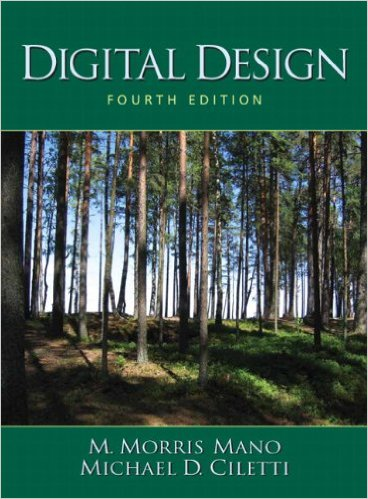
\includegraphics[width=.3\textheight]{FrontMatter/Mano.jpg}},{}]
\bibentry{Mano2007DigDes}
\end{window}



\vspace{2.5in}

\textbf{We will proceed as follows:}

\begin{itemize}
  \item Fast introduction (few sections from Chapter 1).

  \item Detailed study of Chapters 2-7; very few sections will be
  skipped. At the end of each chapter Verilog code for some circuits
  will be explained.

  \item If time permits, Chapter 8 will be covered in full or in parts
\end{itemize}

\clearpage

\chapter*{Course Objectives}
This course combines three approaches to teach students Digital
Design, which is the fundamental prerequisite to understand computer design and architecture:


\begin{enumerate}
  \item Theoretical aspects of the subject will be covered in
  lectures, along with exercises in sections. Students, by the end of
  the course, should be able to design, analyze, and implement
  combinational and synchronous digital circuits.

  \item A second objective is to teach students the digital design
  using a Hardware Descriptive Language (HDL). Students by the end of
  the semester will be able to analyze logic circuits with Verilog
  (one of the available HDLs).

  \item A third objective is to develop the practical sense of the
  students through lab. experiments. Students will be able to
  implement logic circuits using breadboards and ICs.
\end{enumerate}

\clearpage
{
\tiny
\settocdepth{subsection}
\tableofcontents
}


%%% Local Variables:
%%% mode: latex
%%% TeX-master: "../LectureNotesCS221"
%%% End:


\mainmatter

\setcounter{secnumdepth}{3}

\chapter{Introduction}

\clearpage
\section{Mathematical optimization}

\clearpage
\section{Least-squares and linear programming}

\clearpage
\section{Convex optimization}

\clearpage
\section{Nonlinear optimization}

\clearpage
\section{Outline}

\clearpage
\section{Notation}


\clearpage
\hfil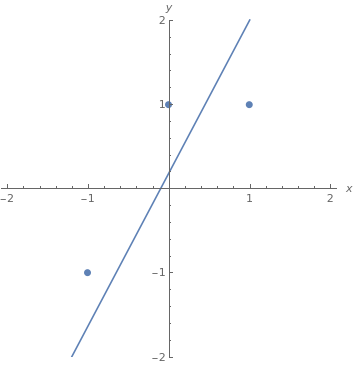
\includegraphics[width=.5\textwidth]{../Graphics/01-ML01.png}\hfil

\clearpage
\hfil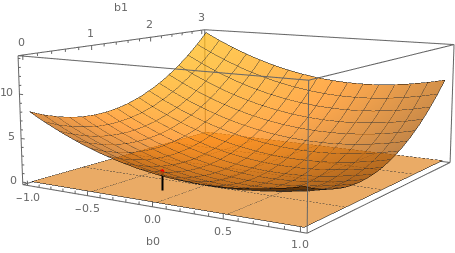
\includegraphics[width=.5\textwidth]{../Graphics/01-ML02.png}\hfil

\clearpage
\hfil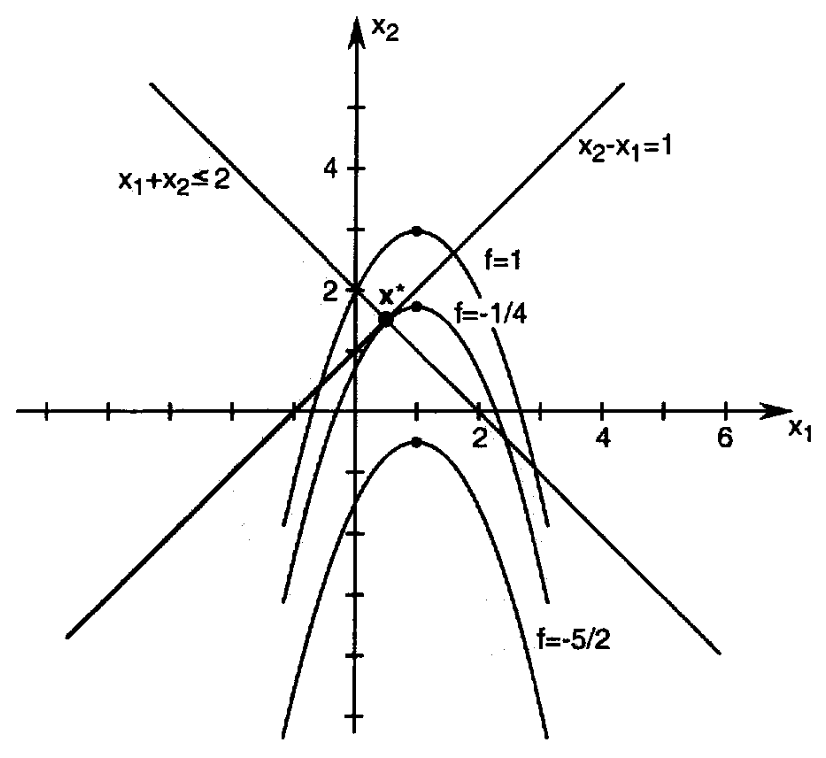
\includegraphics[width=.5\textwidth]{../Graphics/ChongFigure20_1.png}\hfil

%%% Local Variables:
%%% mode: latex
%%% TeX-master: "../LectureNotes-Optimization"
%%% End:



\chapter{Convex sets}

\clearpage
\section{Affine and convex sets}

\clearpage
\section{Some important examples}

\clearpage
\section{Operations that preserve convexity}

\clearpage
\section{Generalized inequalities}

\clearpage
\section{Separating and supporting hyperplanes}

\clearpage
\section{Dual cones and generalized inequalities}


\clearpage
\hfil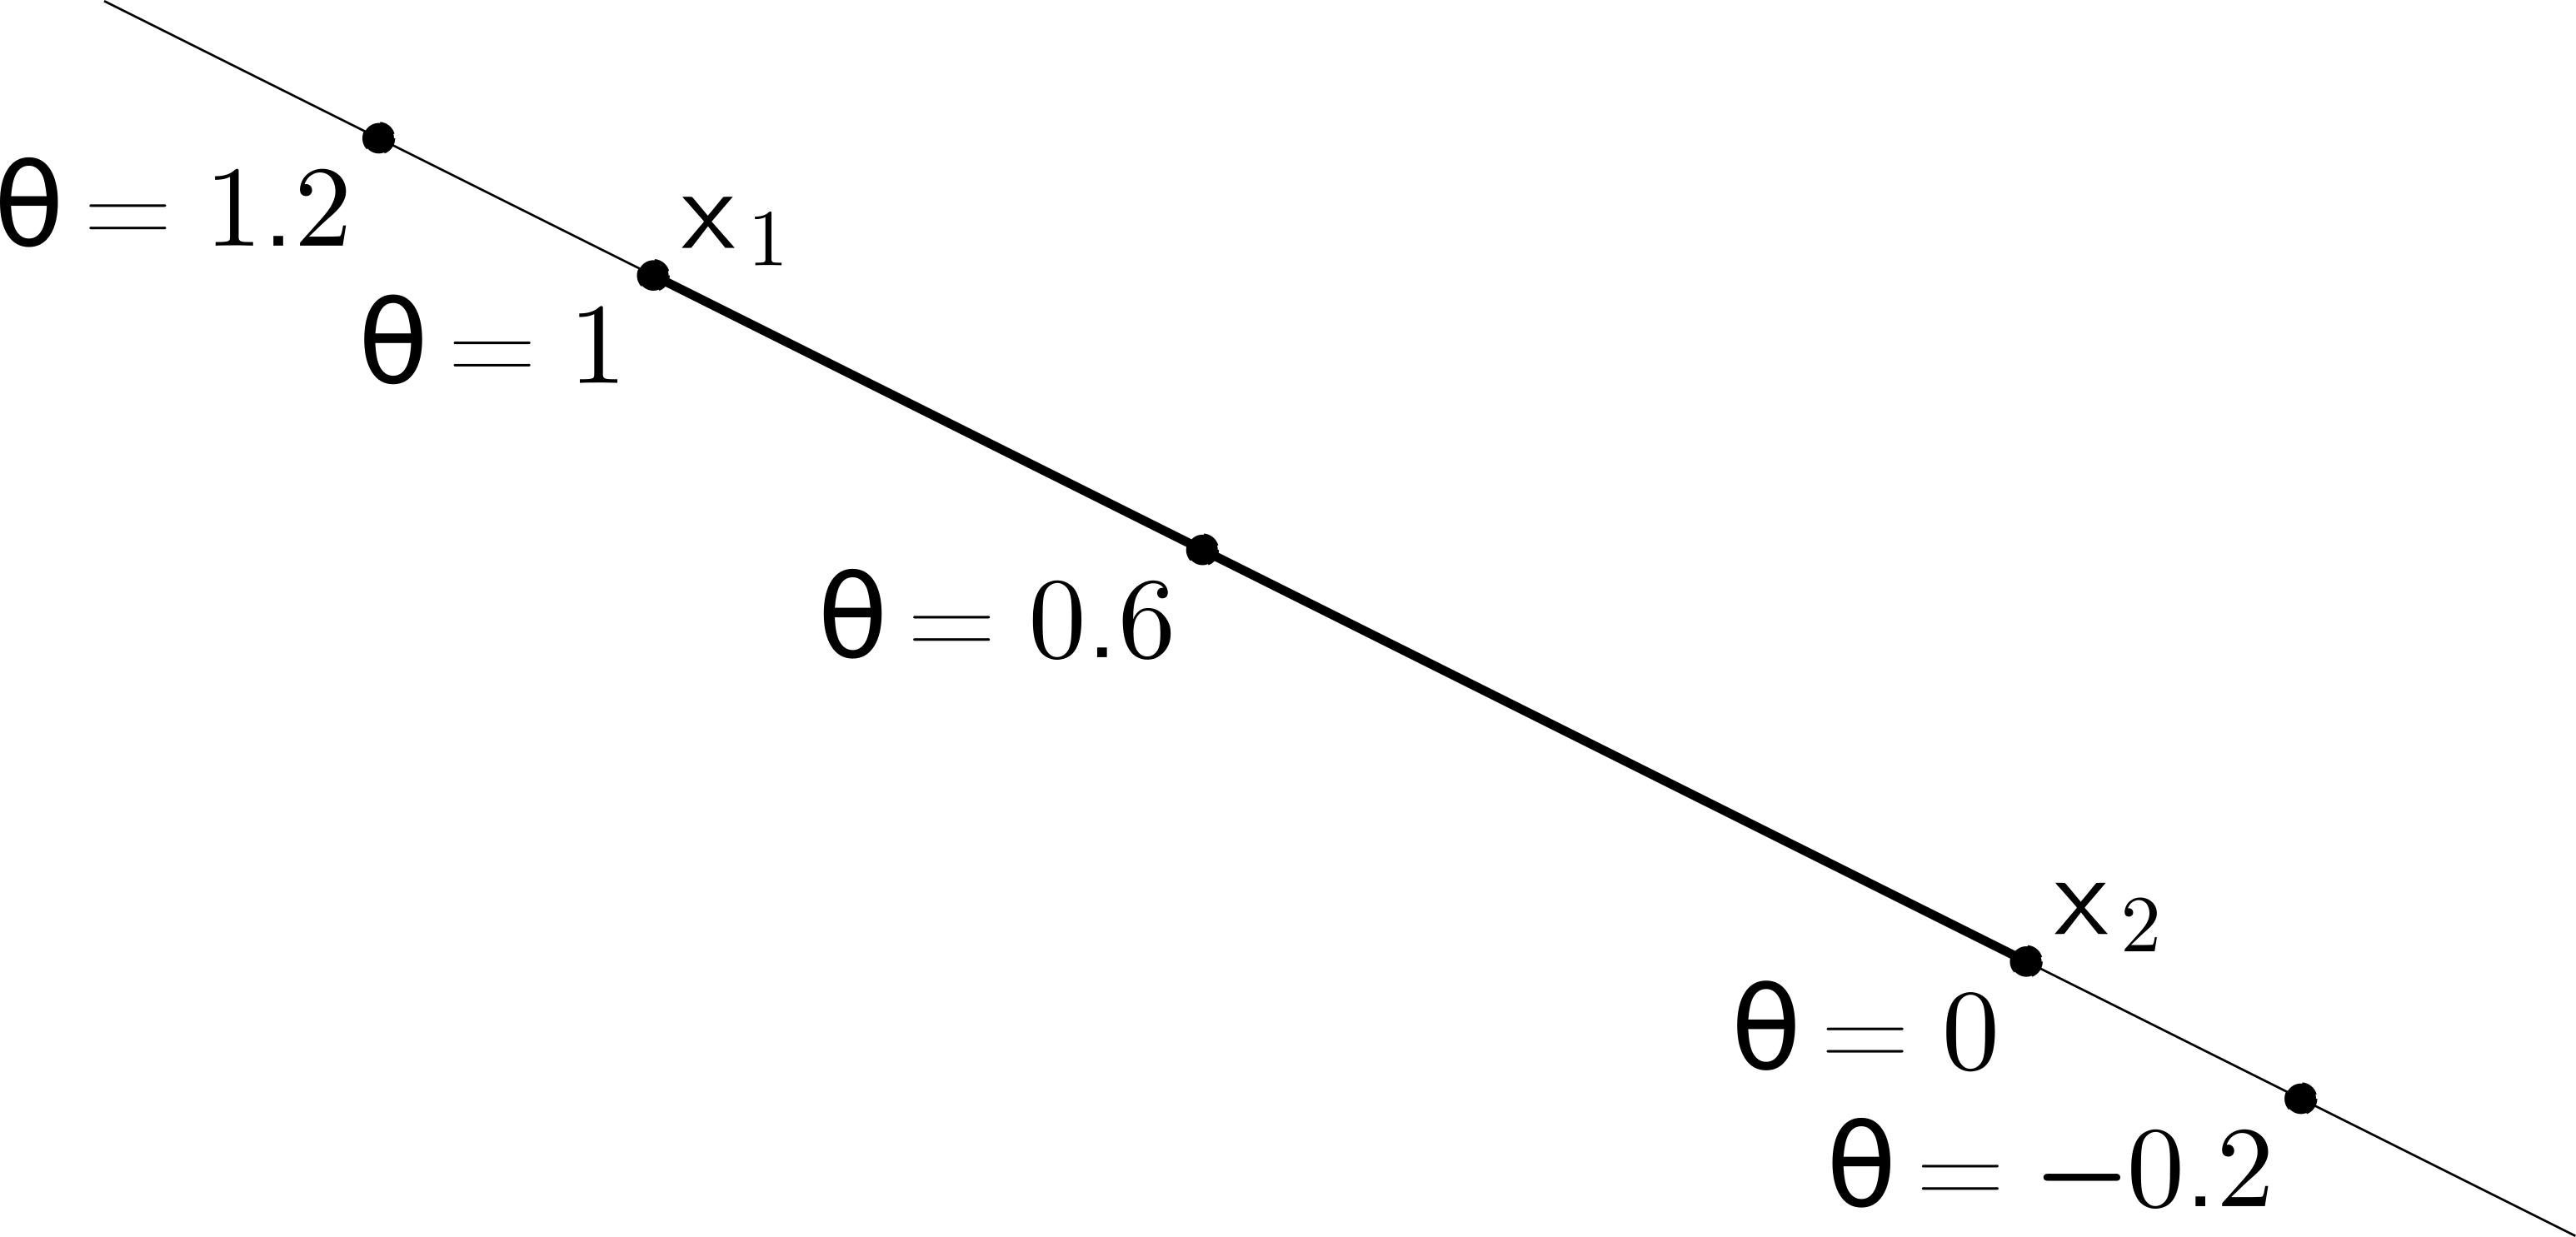
\includegraphics[width=.5\textwidth]{../Graphics/022.png}\hfil

\clearpage
\hfil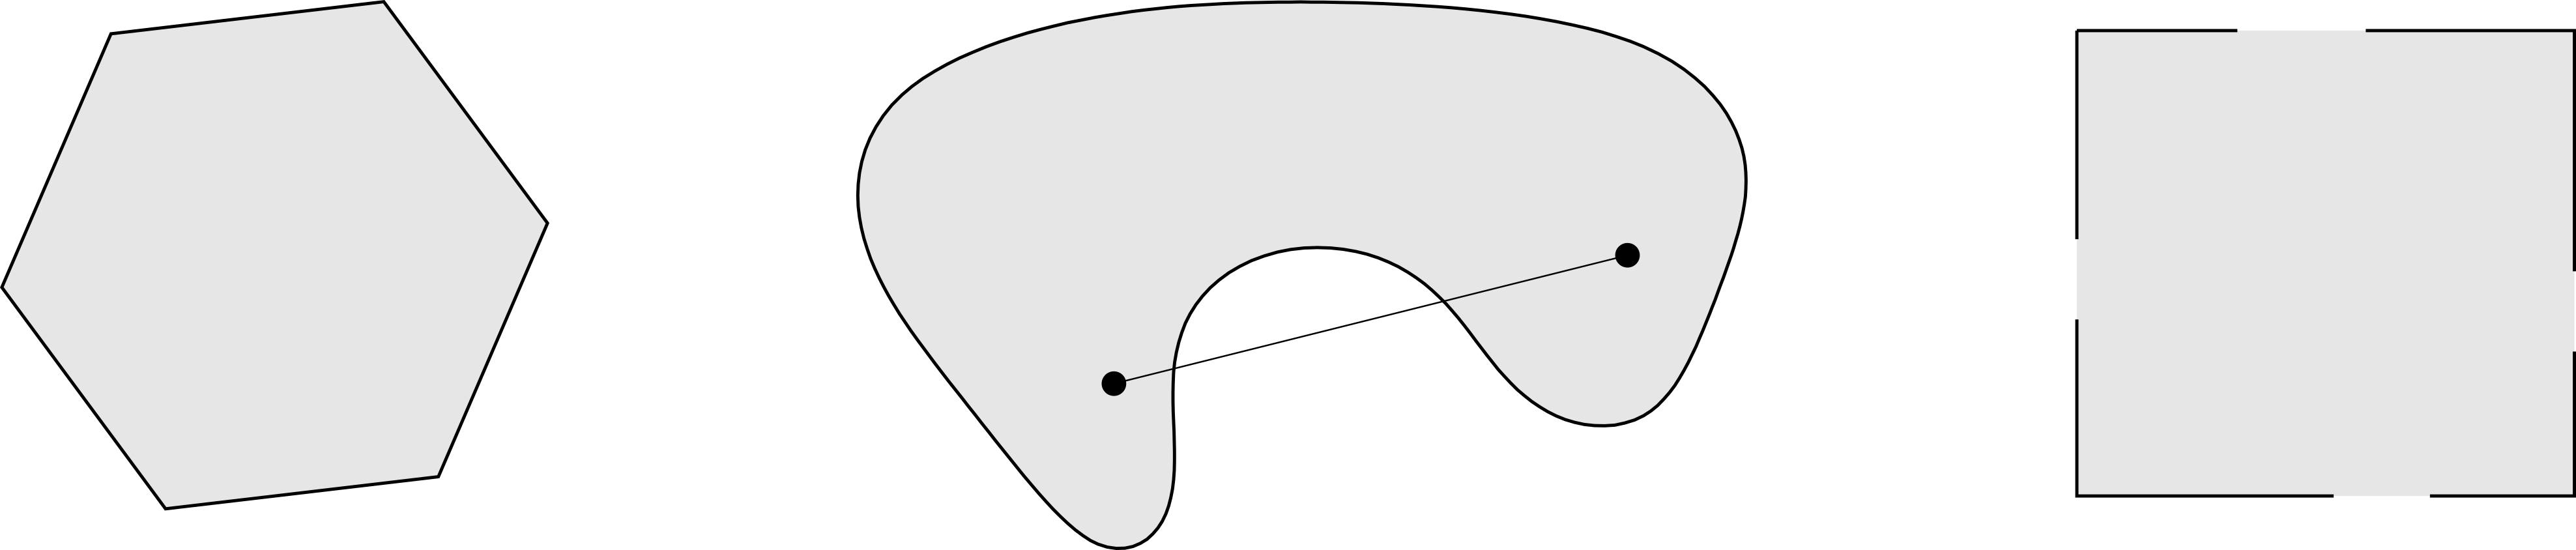
\includegraphics[width=.5\textwidth]{../Graphics/024a.png}\hfil

\clearpage
\hfil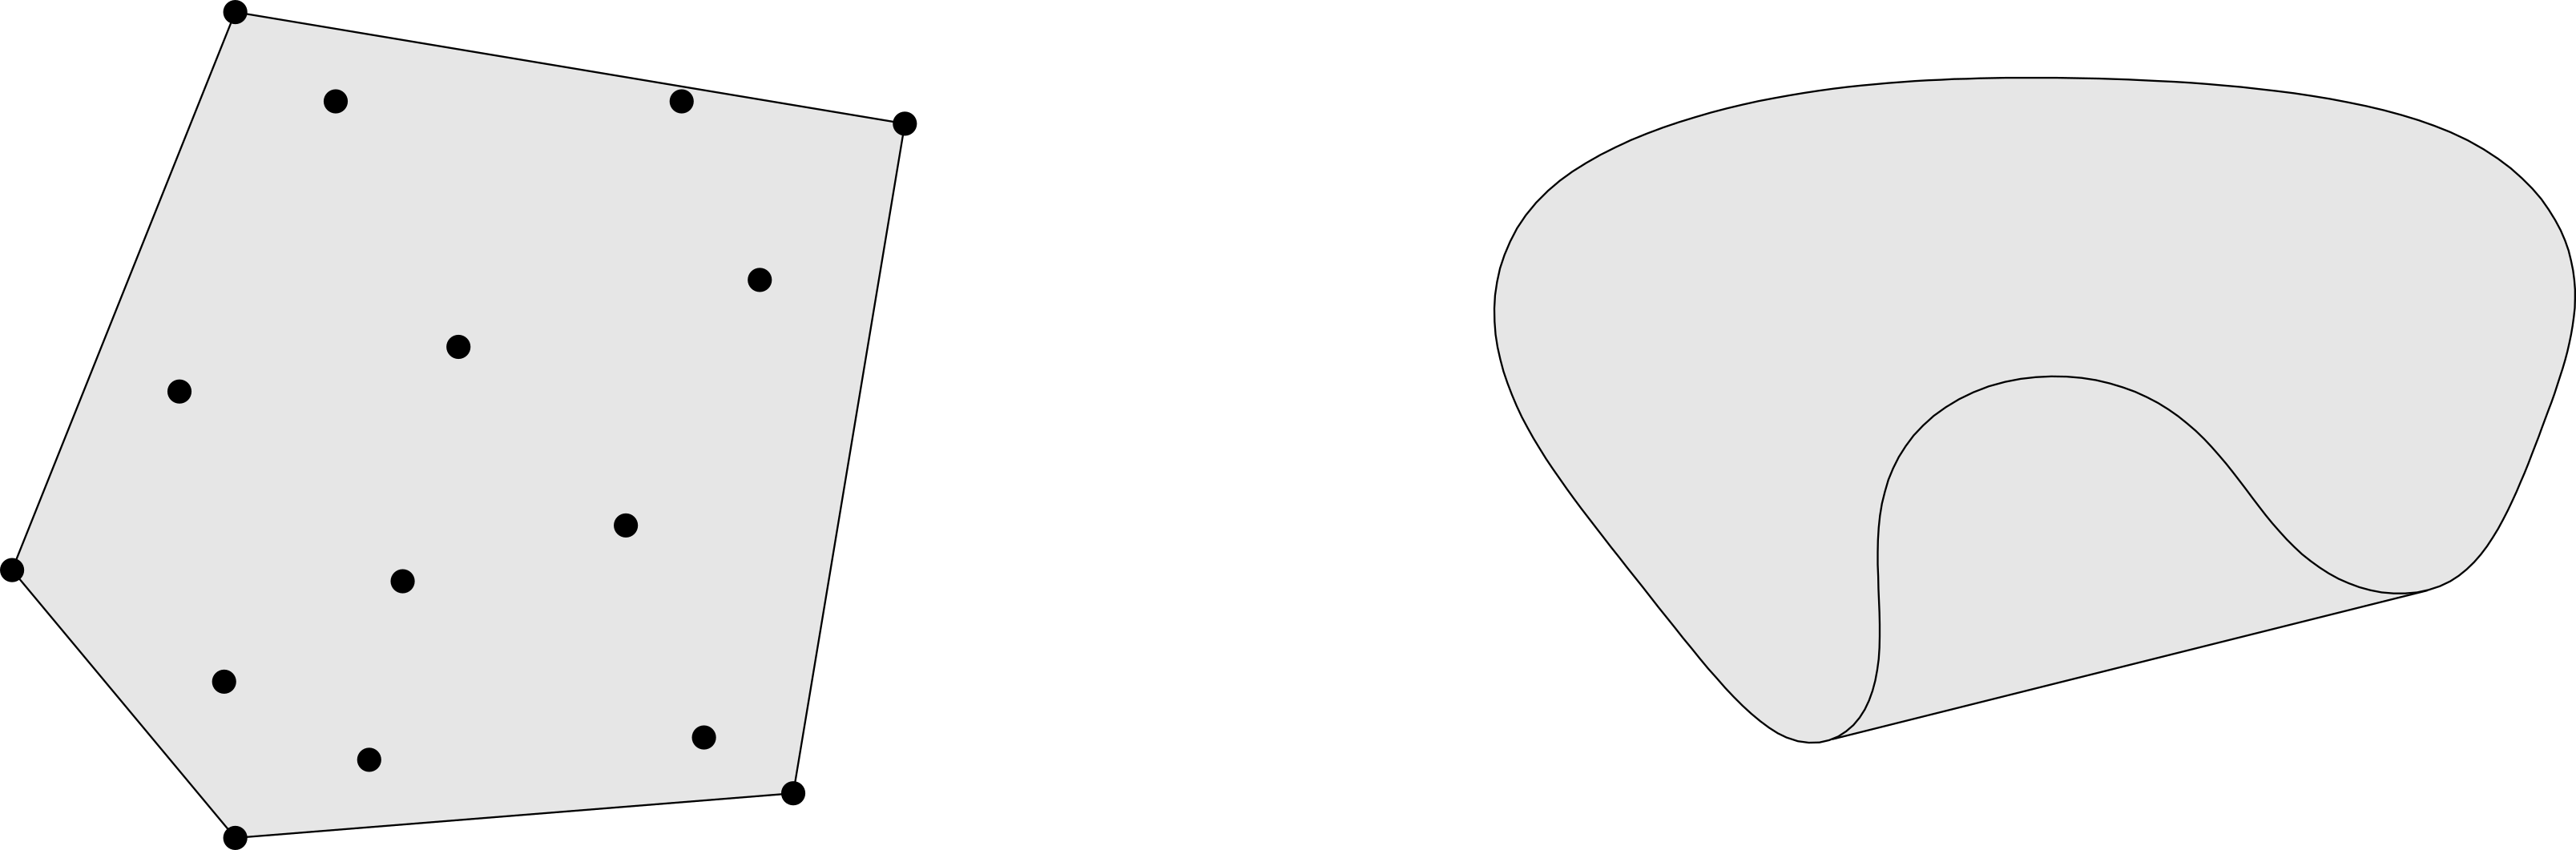
\includegraphics[width=.5\textwidth]{../Graphics/024b.png}\hfil

\clearpage
\hfil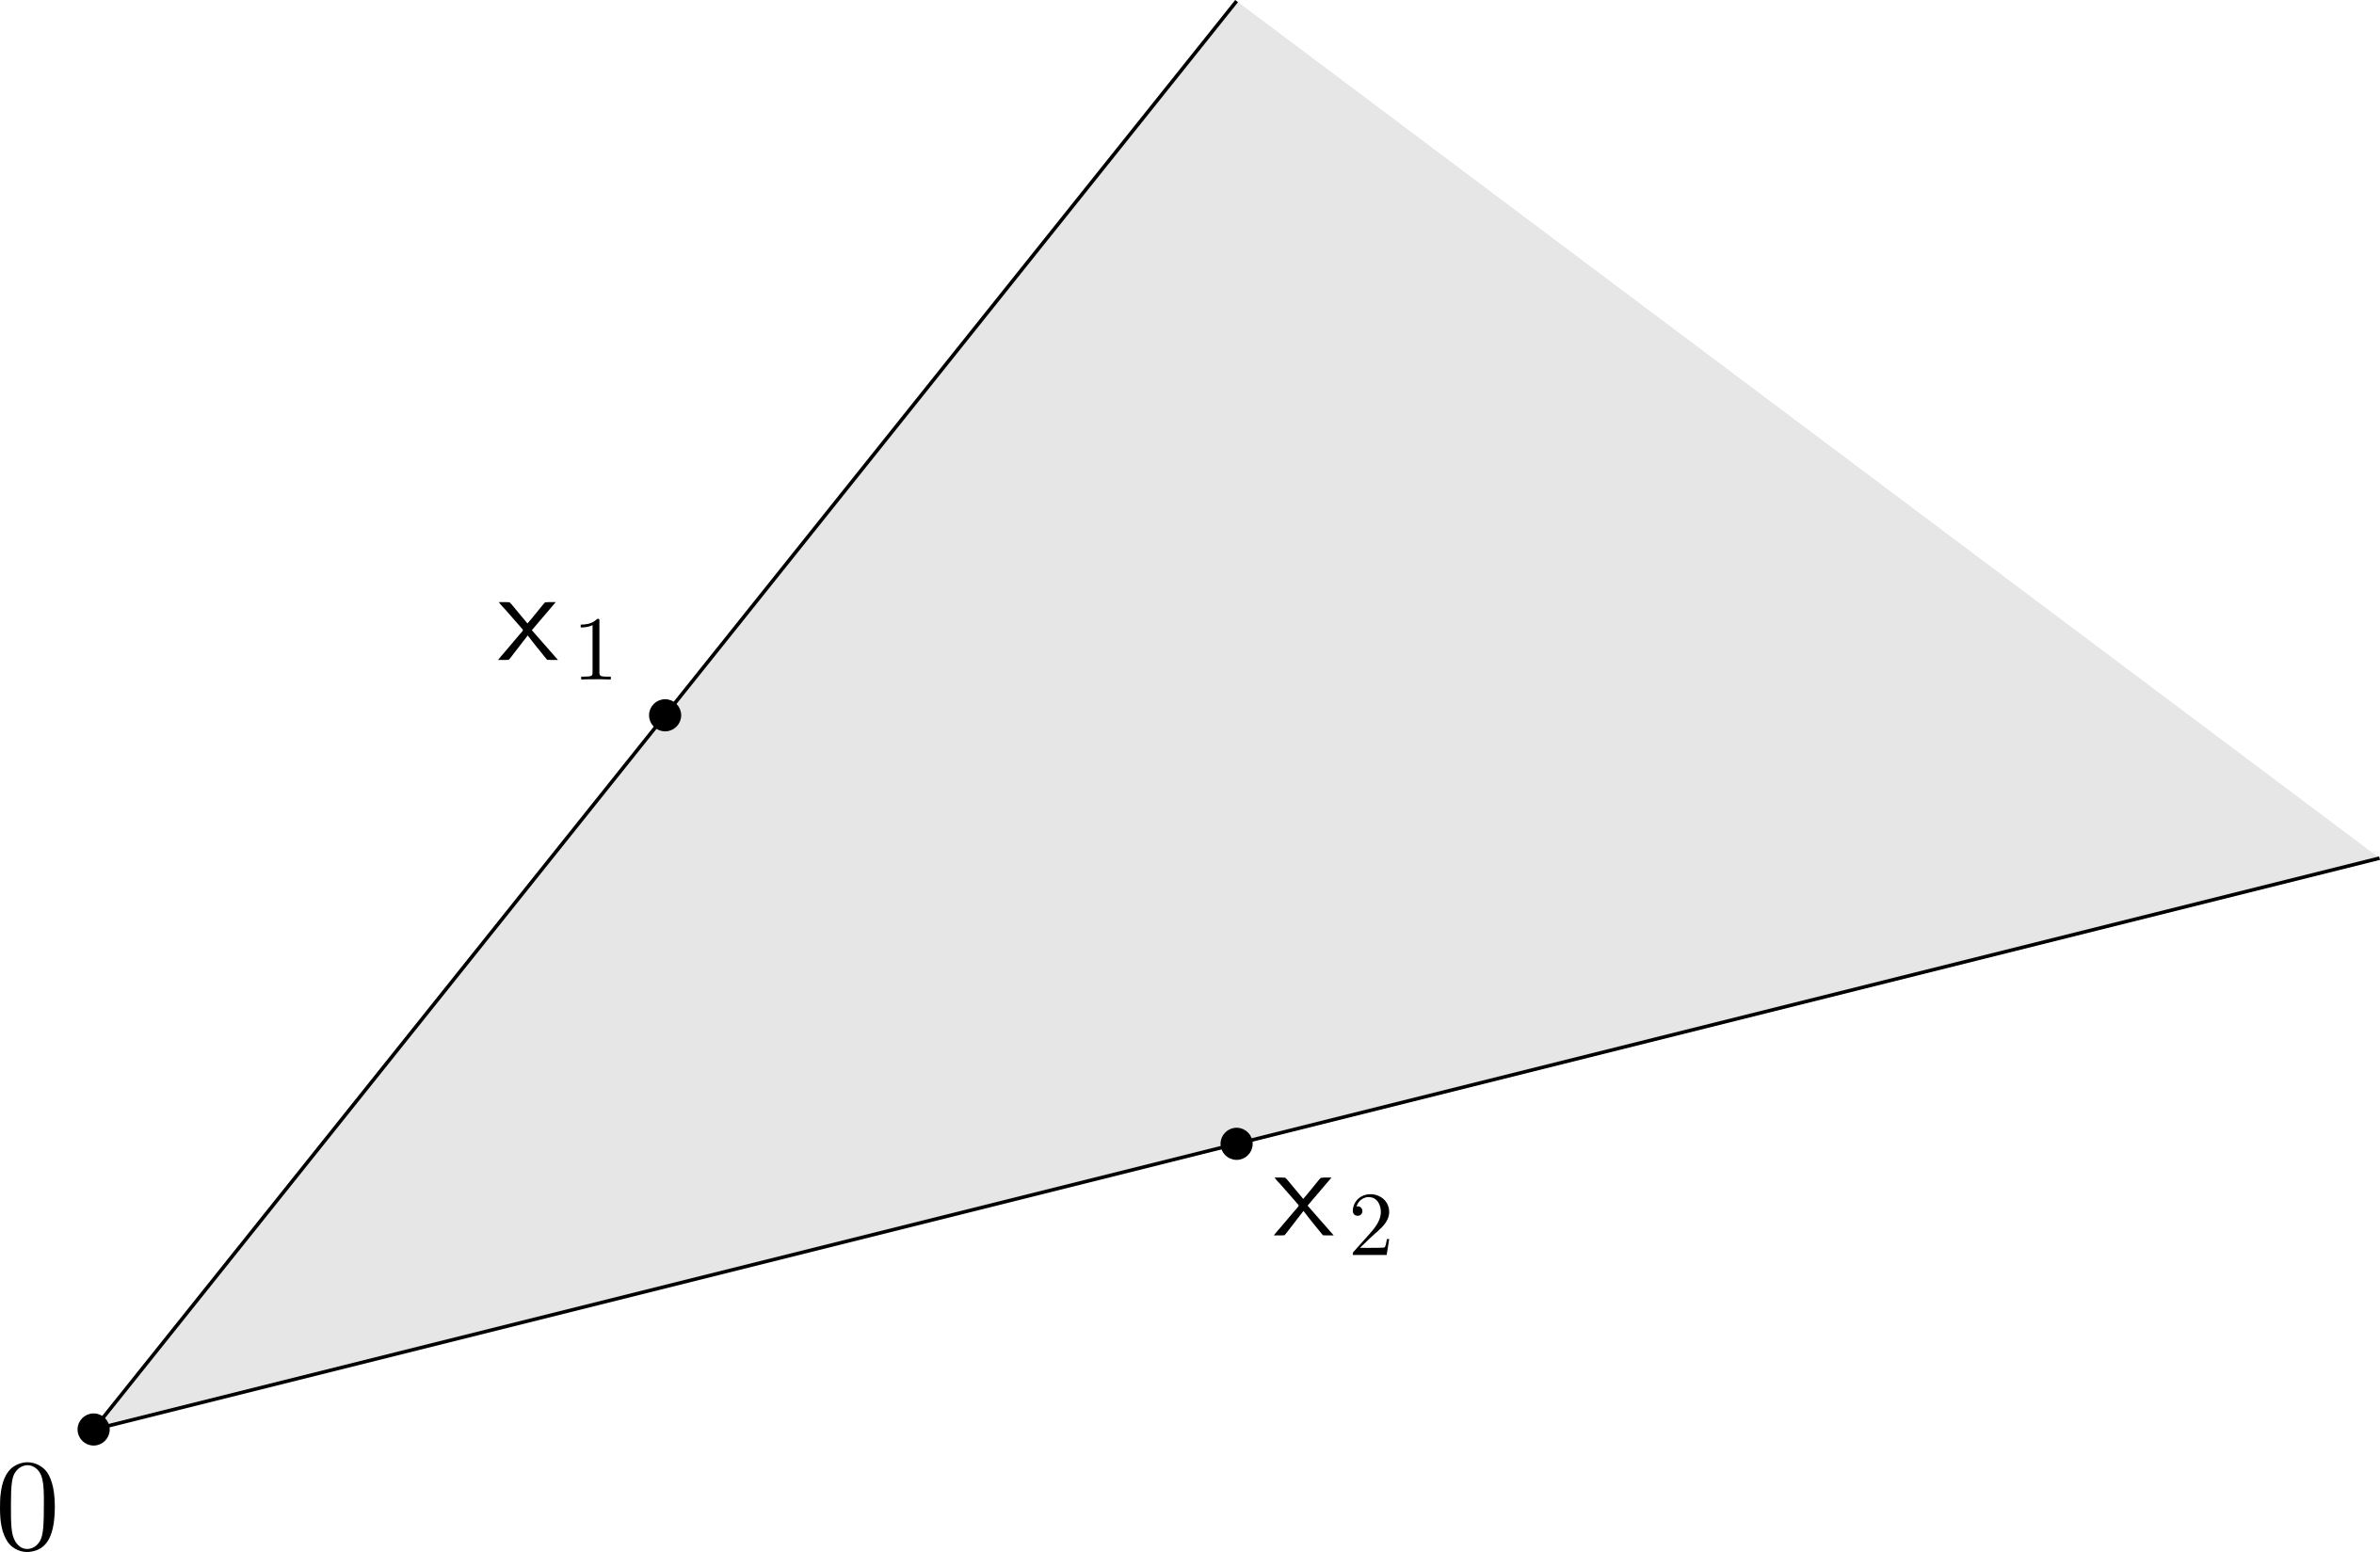
\includegraphics[width=.5\textwidth]{../Graphics/026a.png}\hfil

\clearpage
\hfil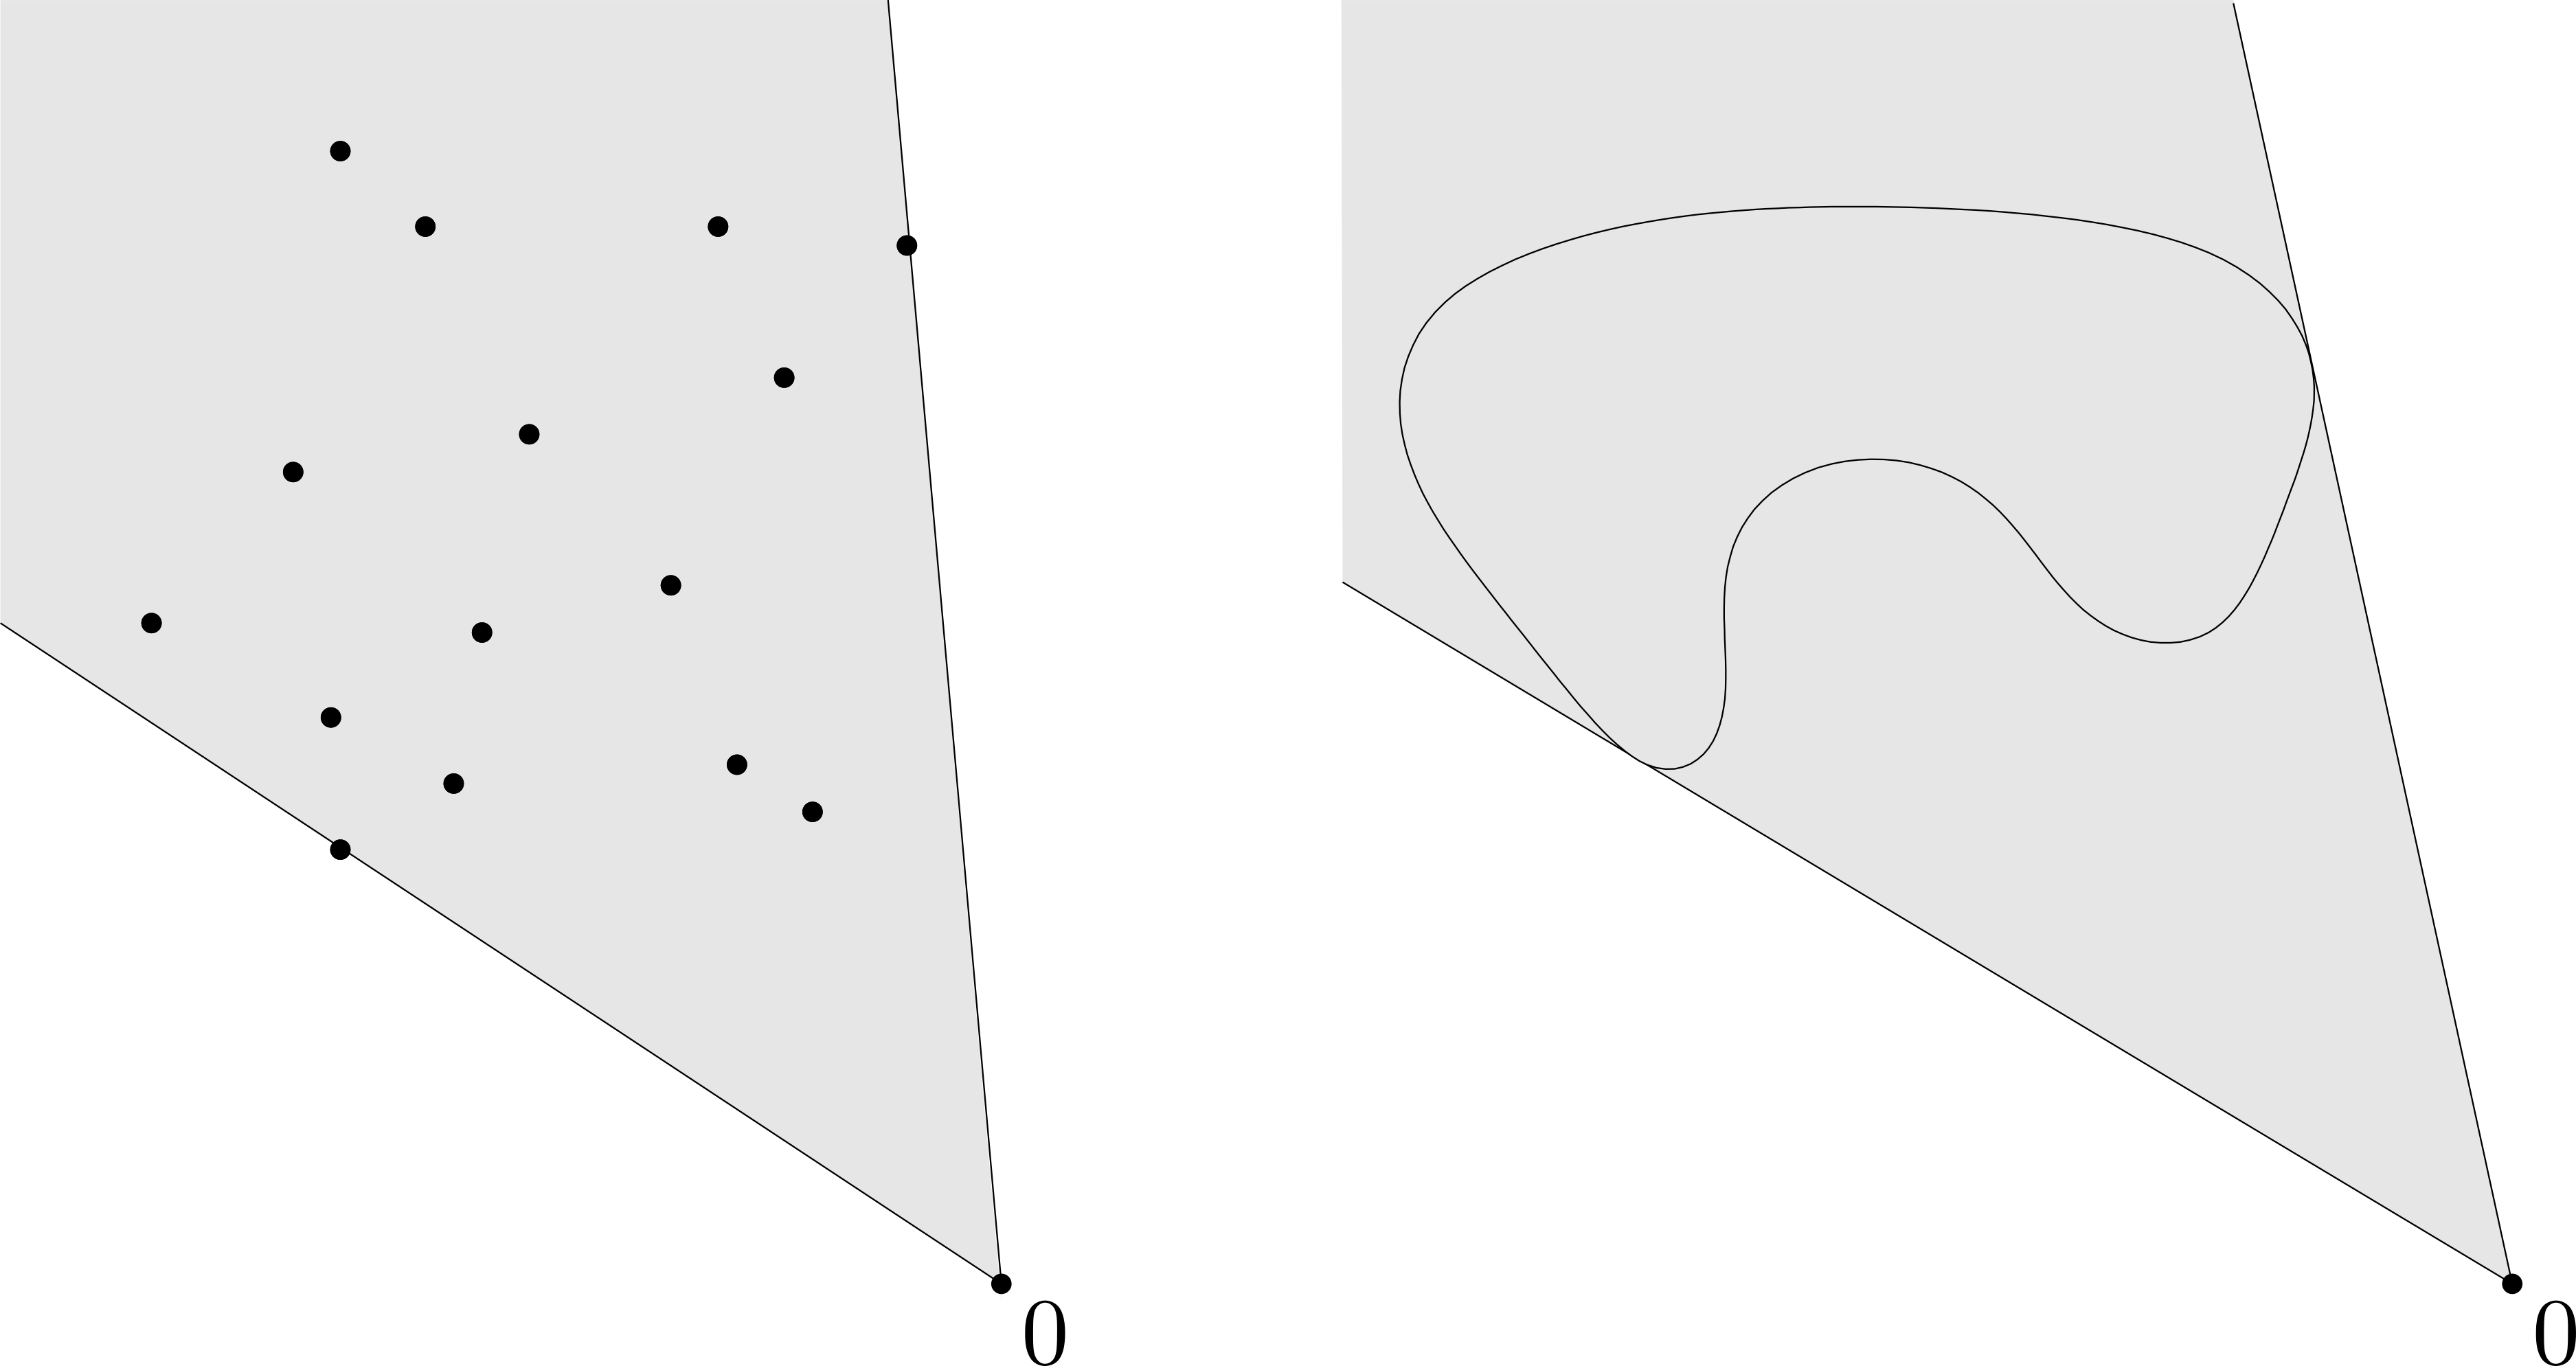
\includegraphics[width=.5\textwidth]{../Graphics/026b.png}\hfil

\clearpage
\hfil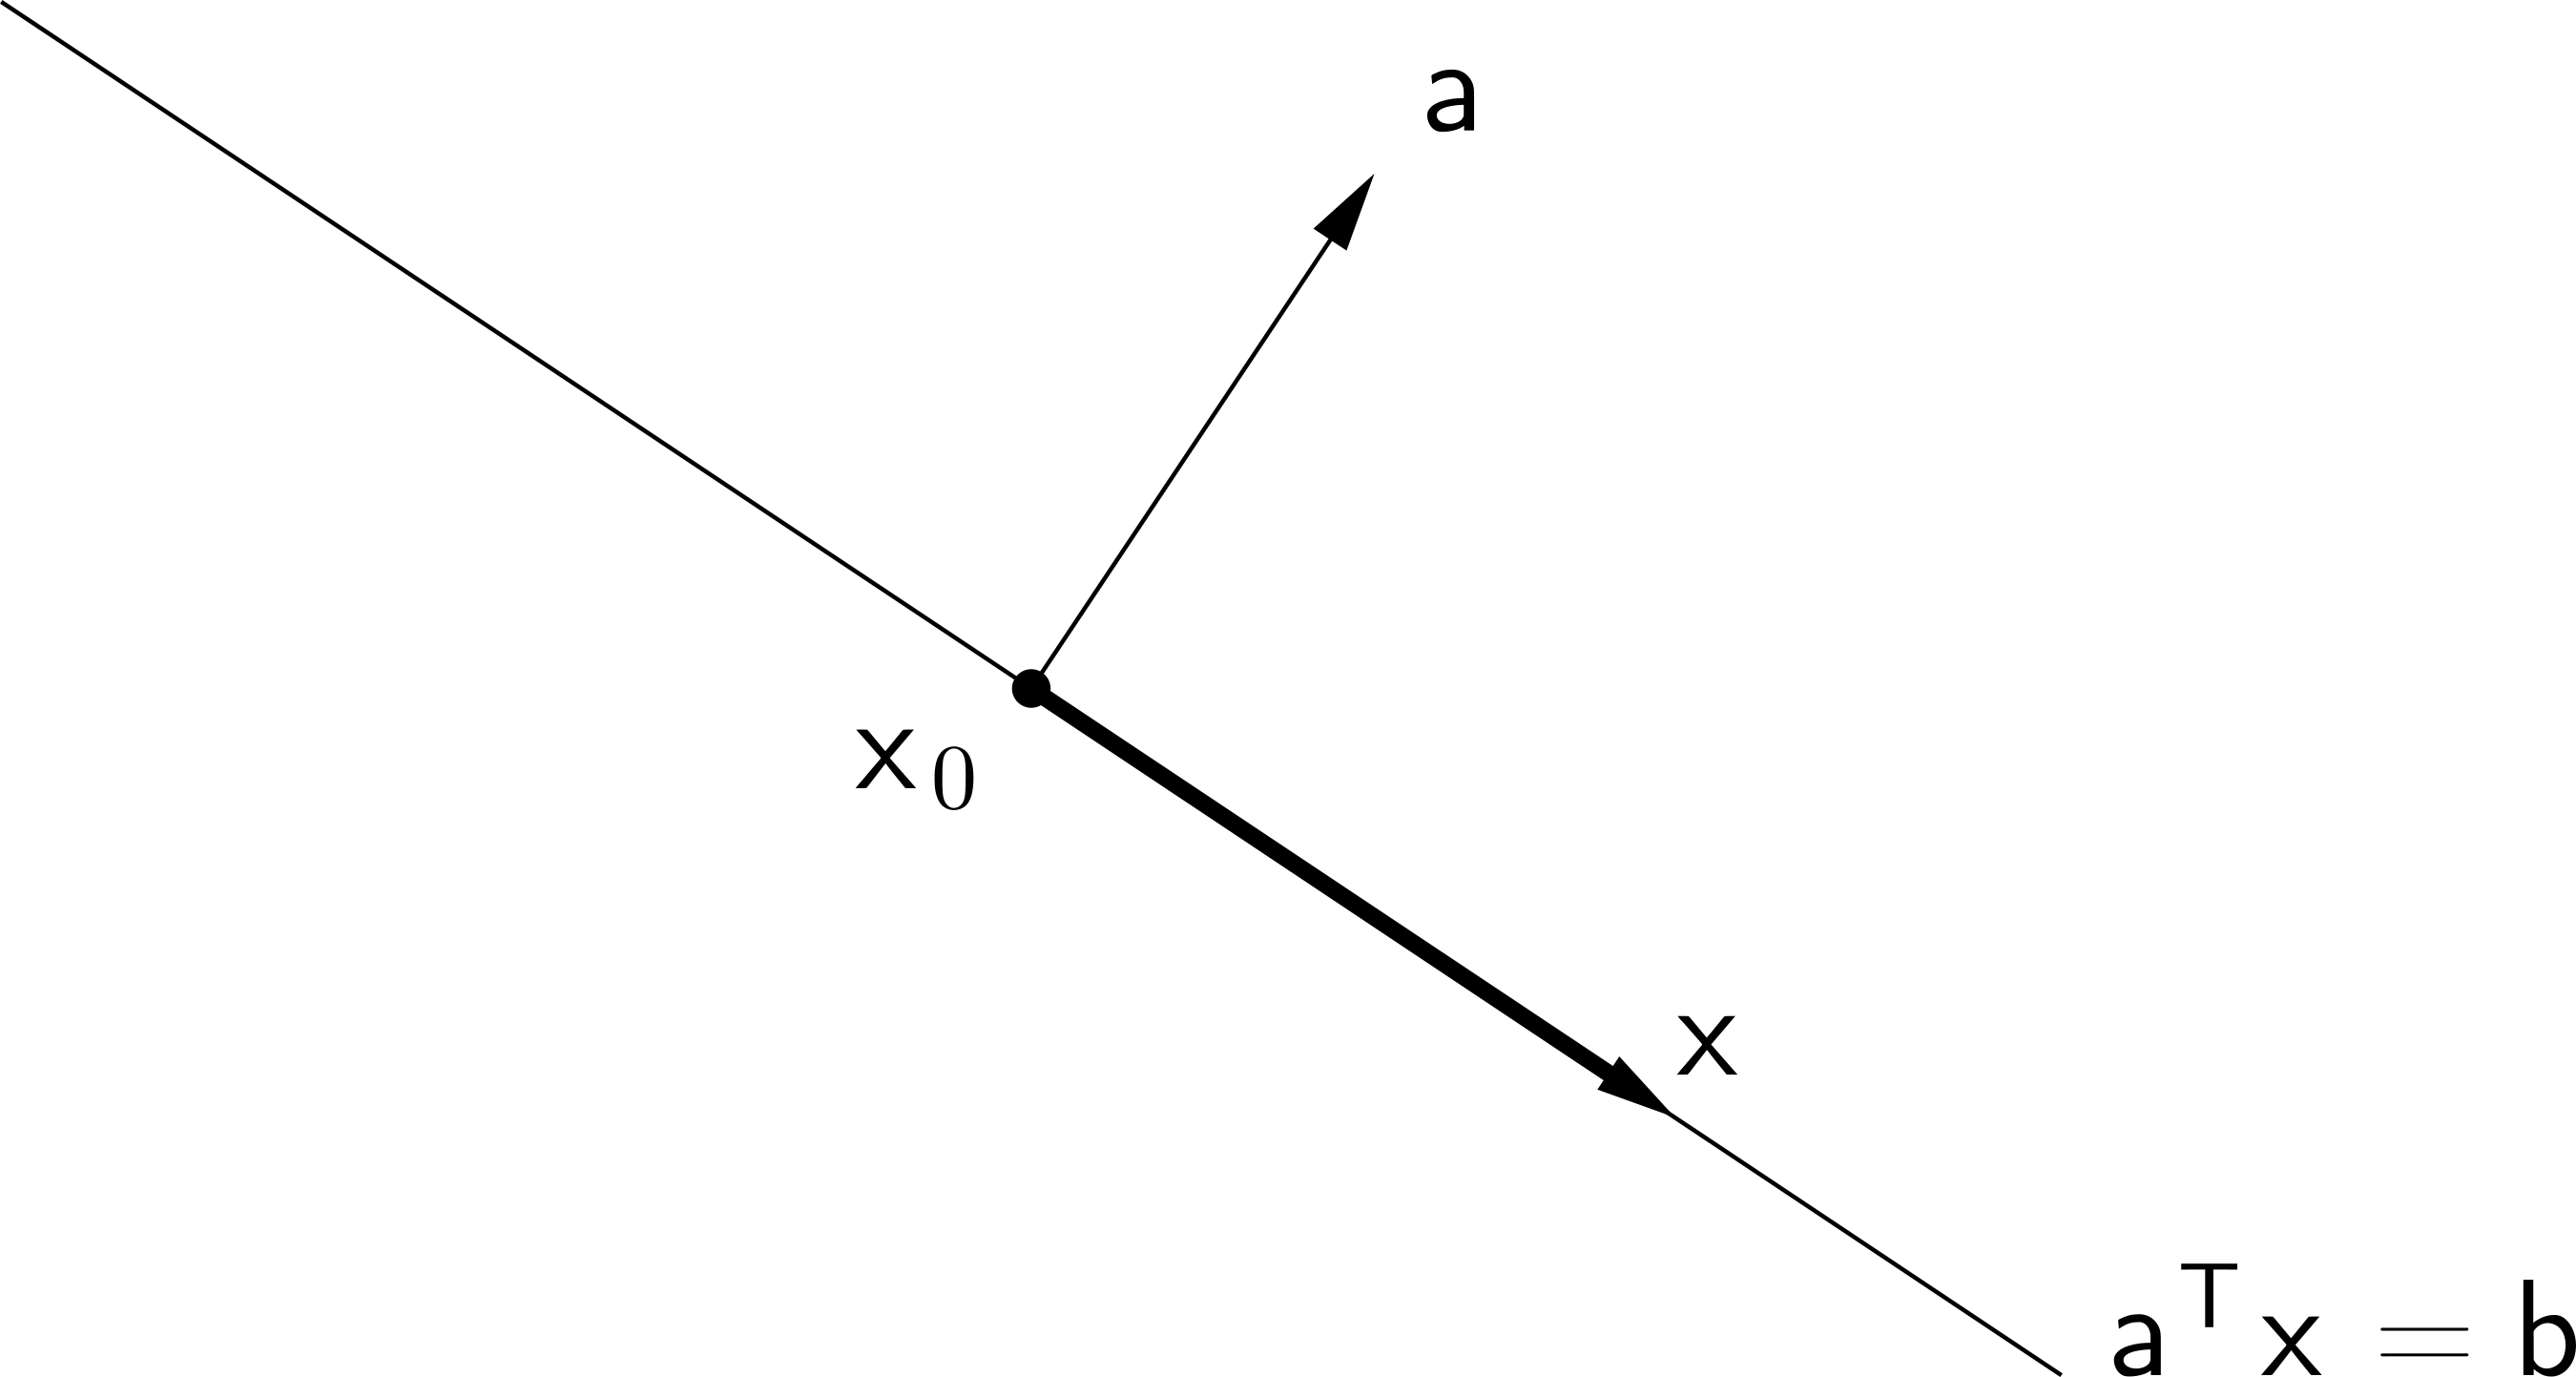
\includegraphics[width=.5\textwidth]{../Graphics/028a.png}\hfil

\clearpage
\hfil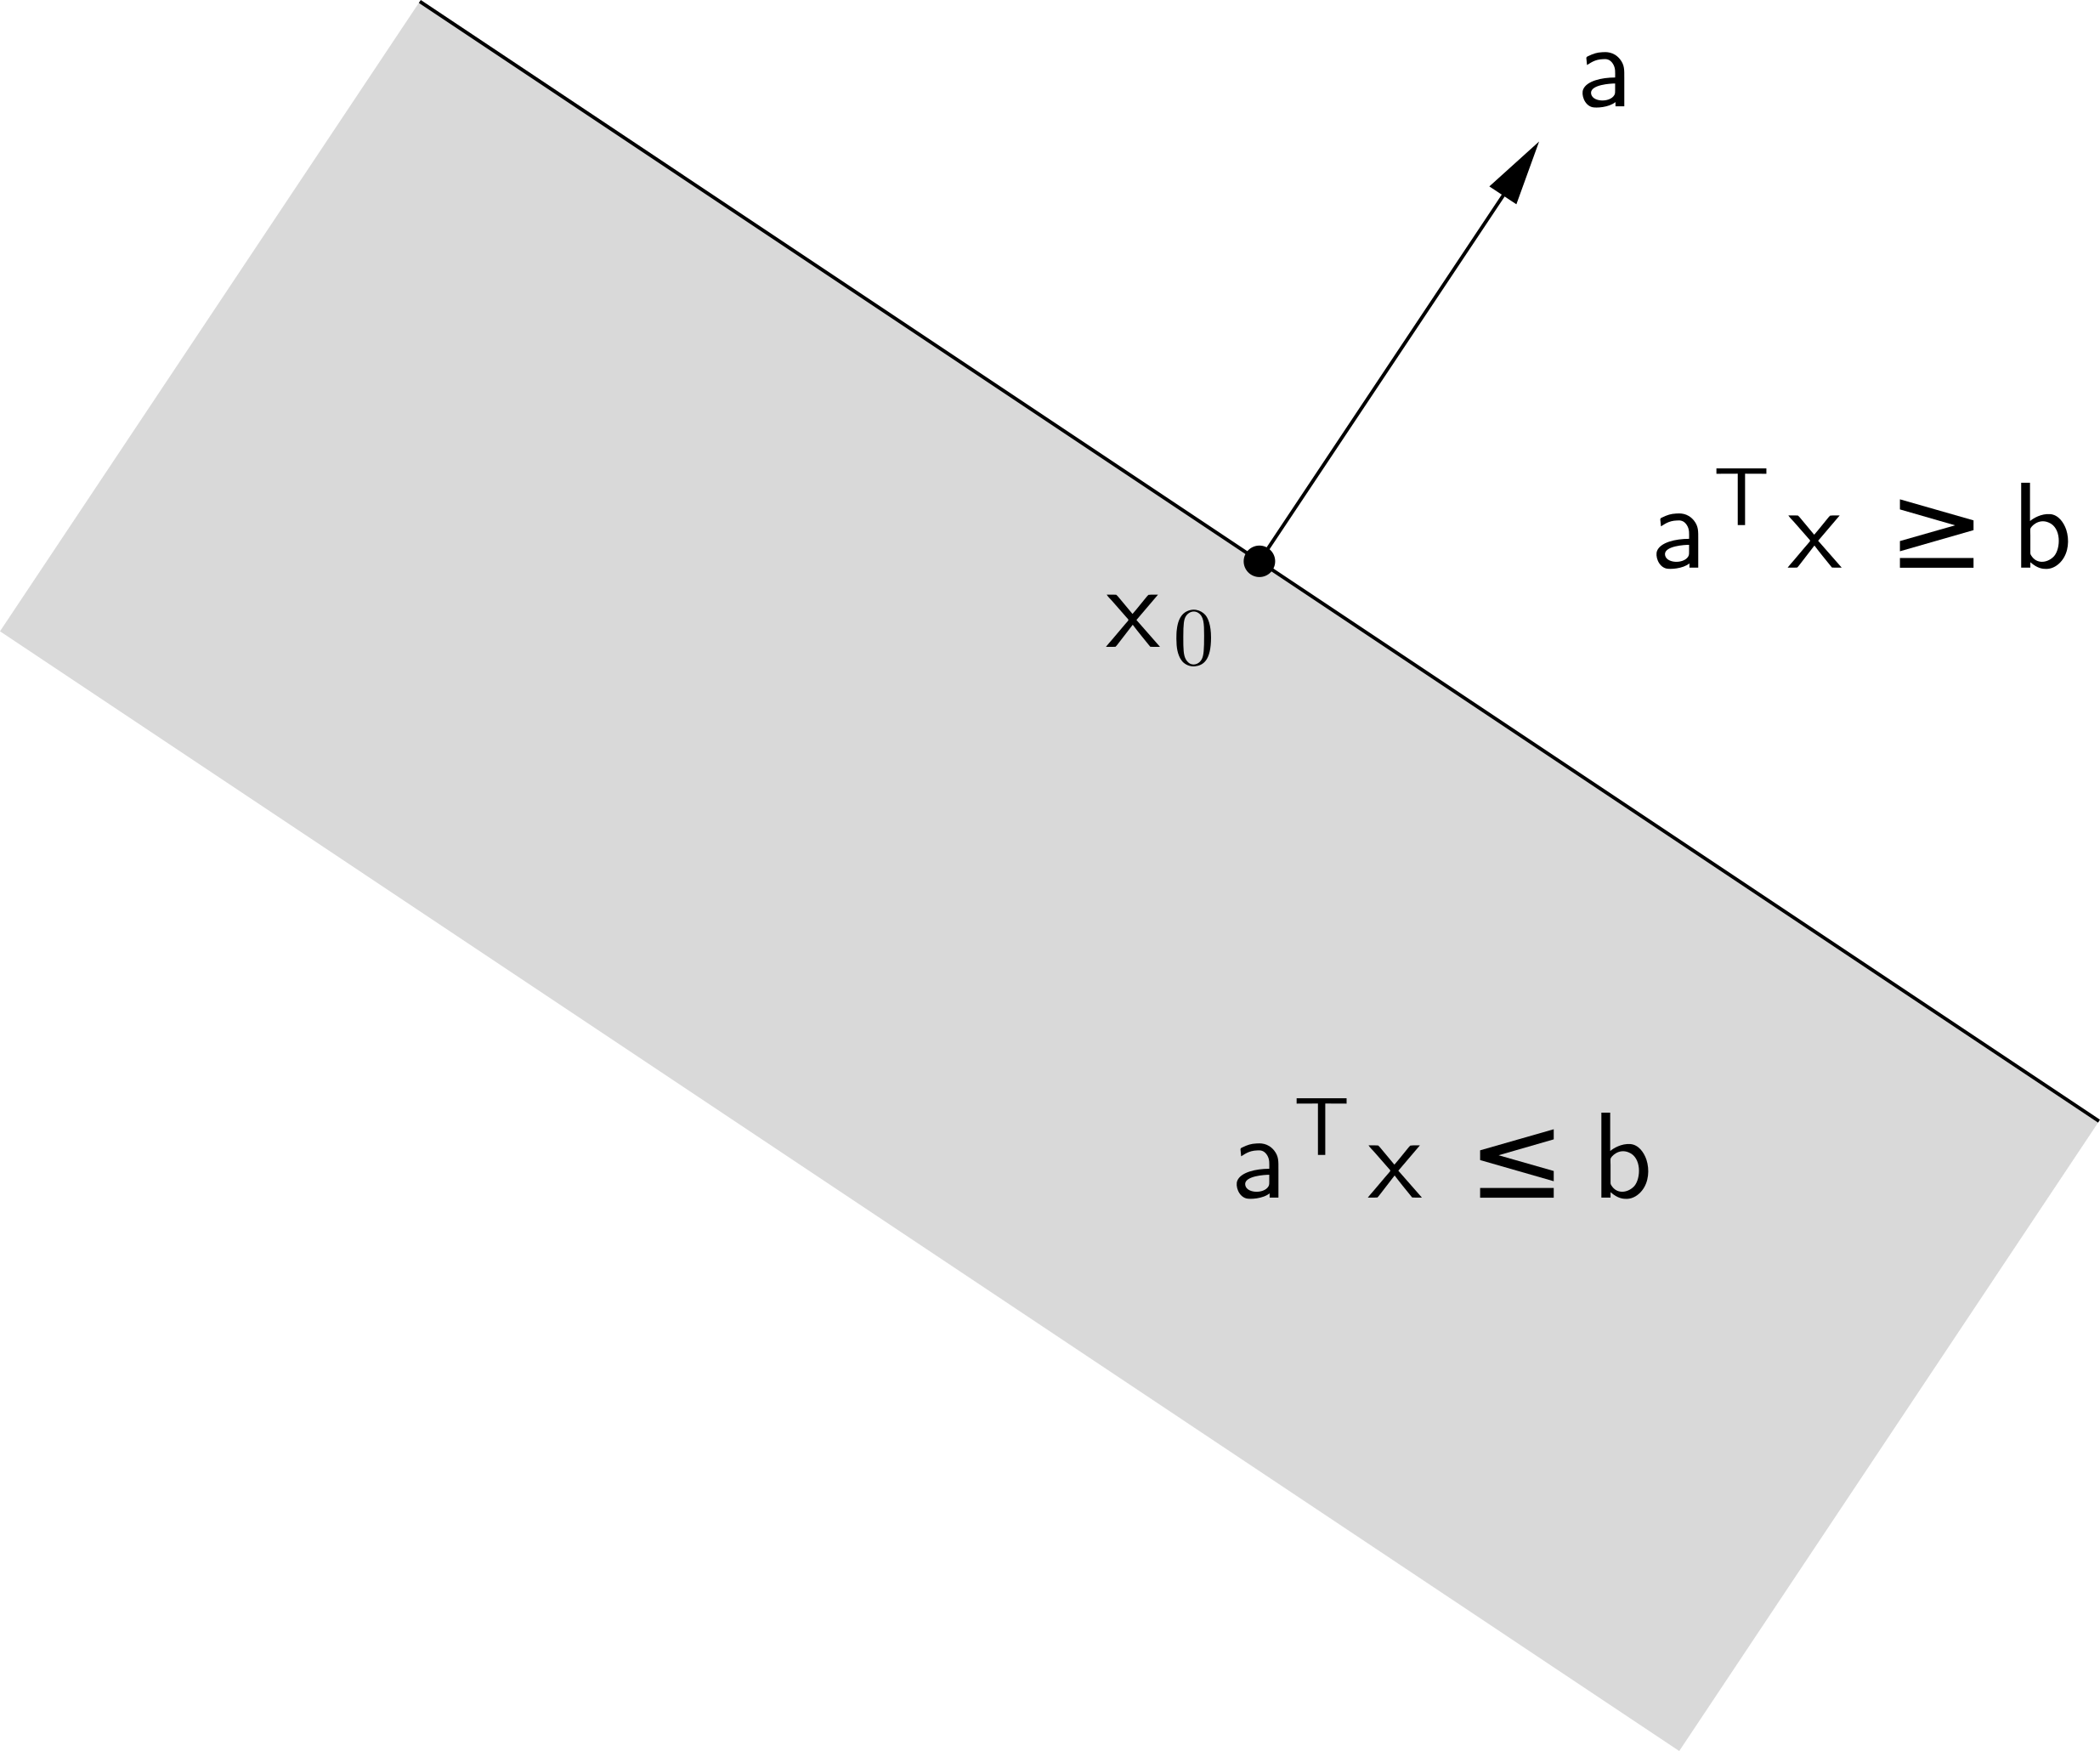
\includegraphics[width=.5\textwidth]{../Graphics/028b.png}\hfil

\clearpage
\hfil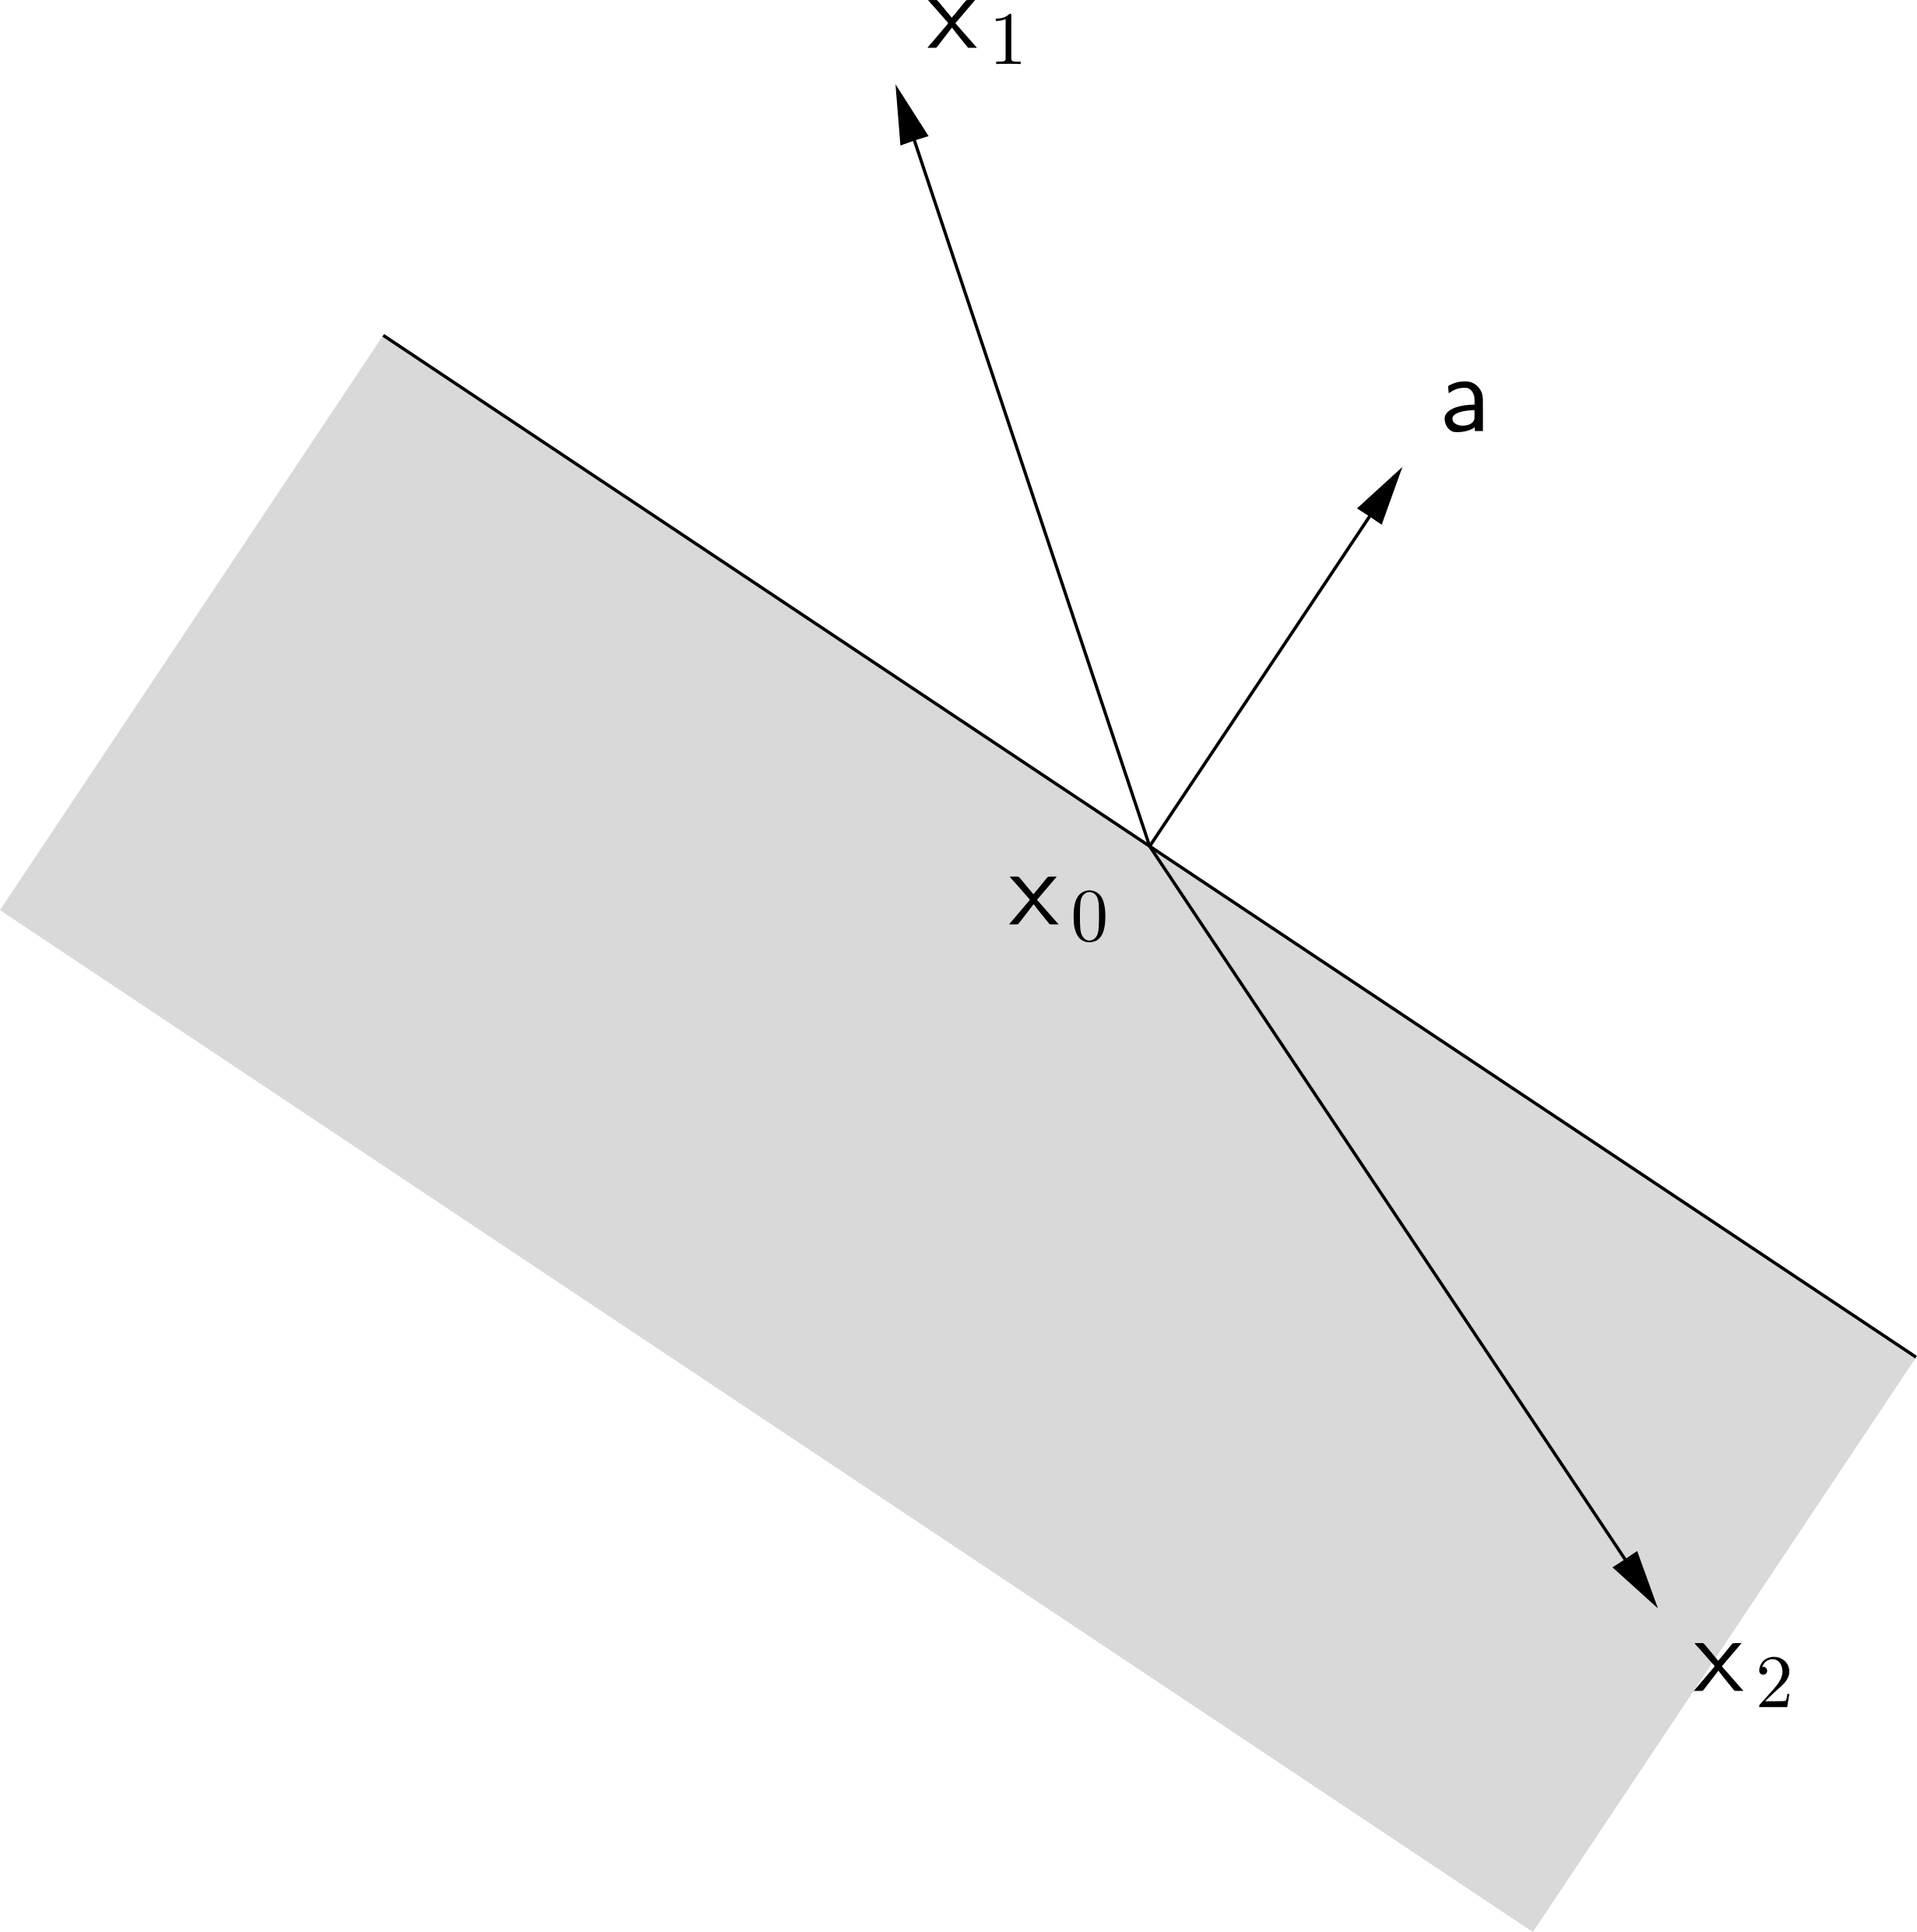
\includegraphics[width=.5\textwidth]{../Graphics/029.png}\hfil

\clearpage
\hfil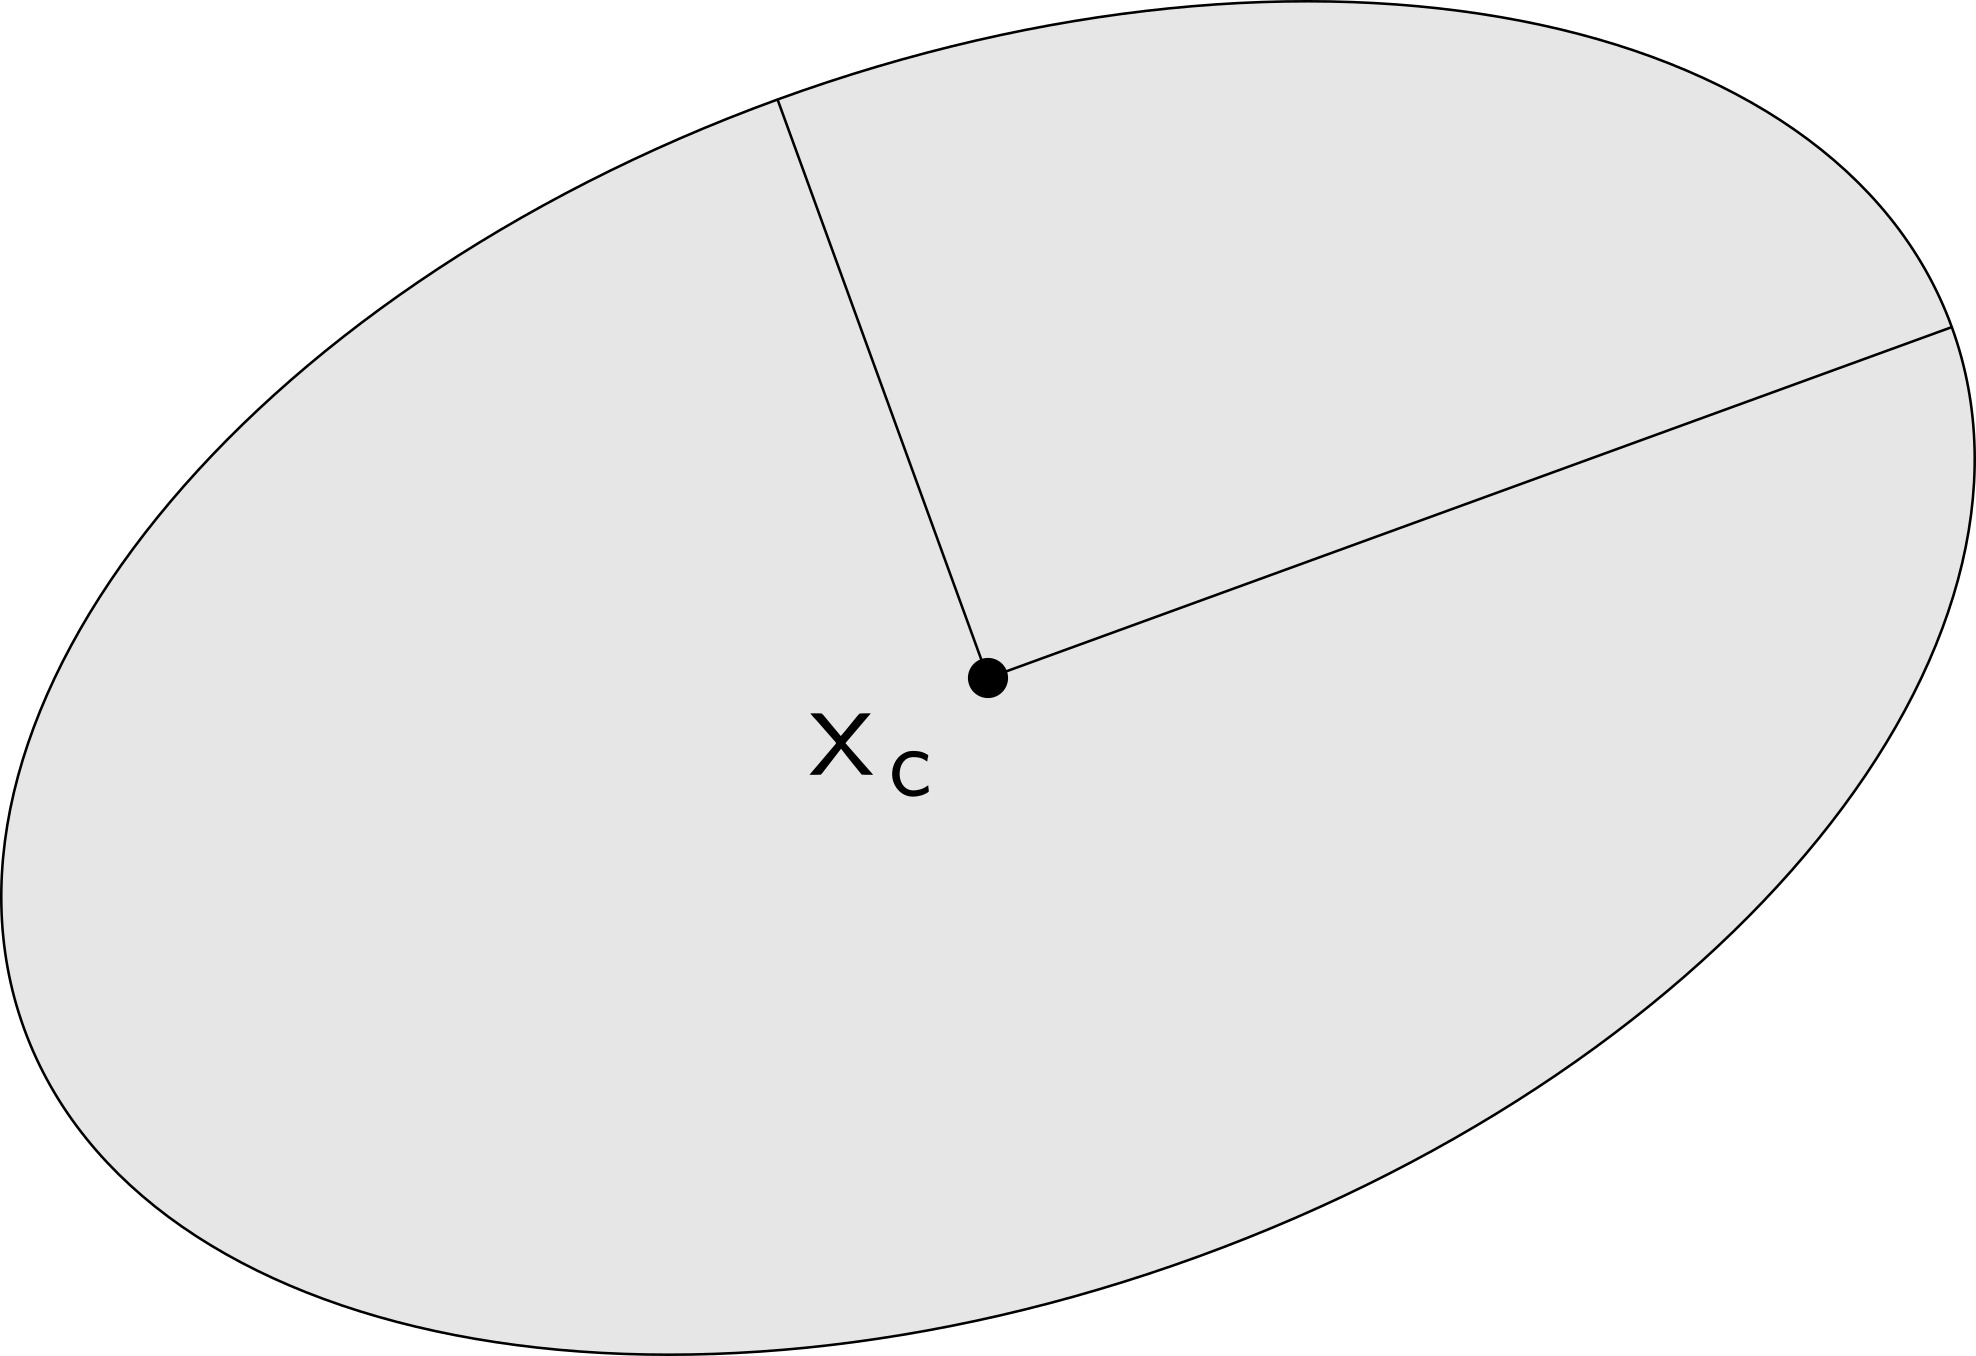
\includegraphics[width=.5\textwidth]{../Graphics/030.png}\hfil

\clearpage
\hfil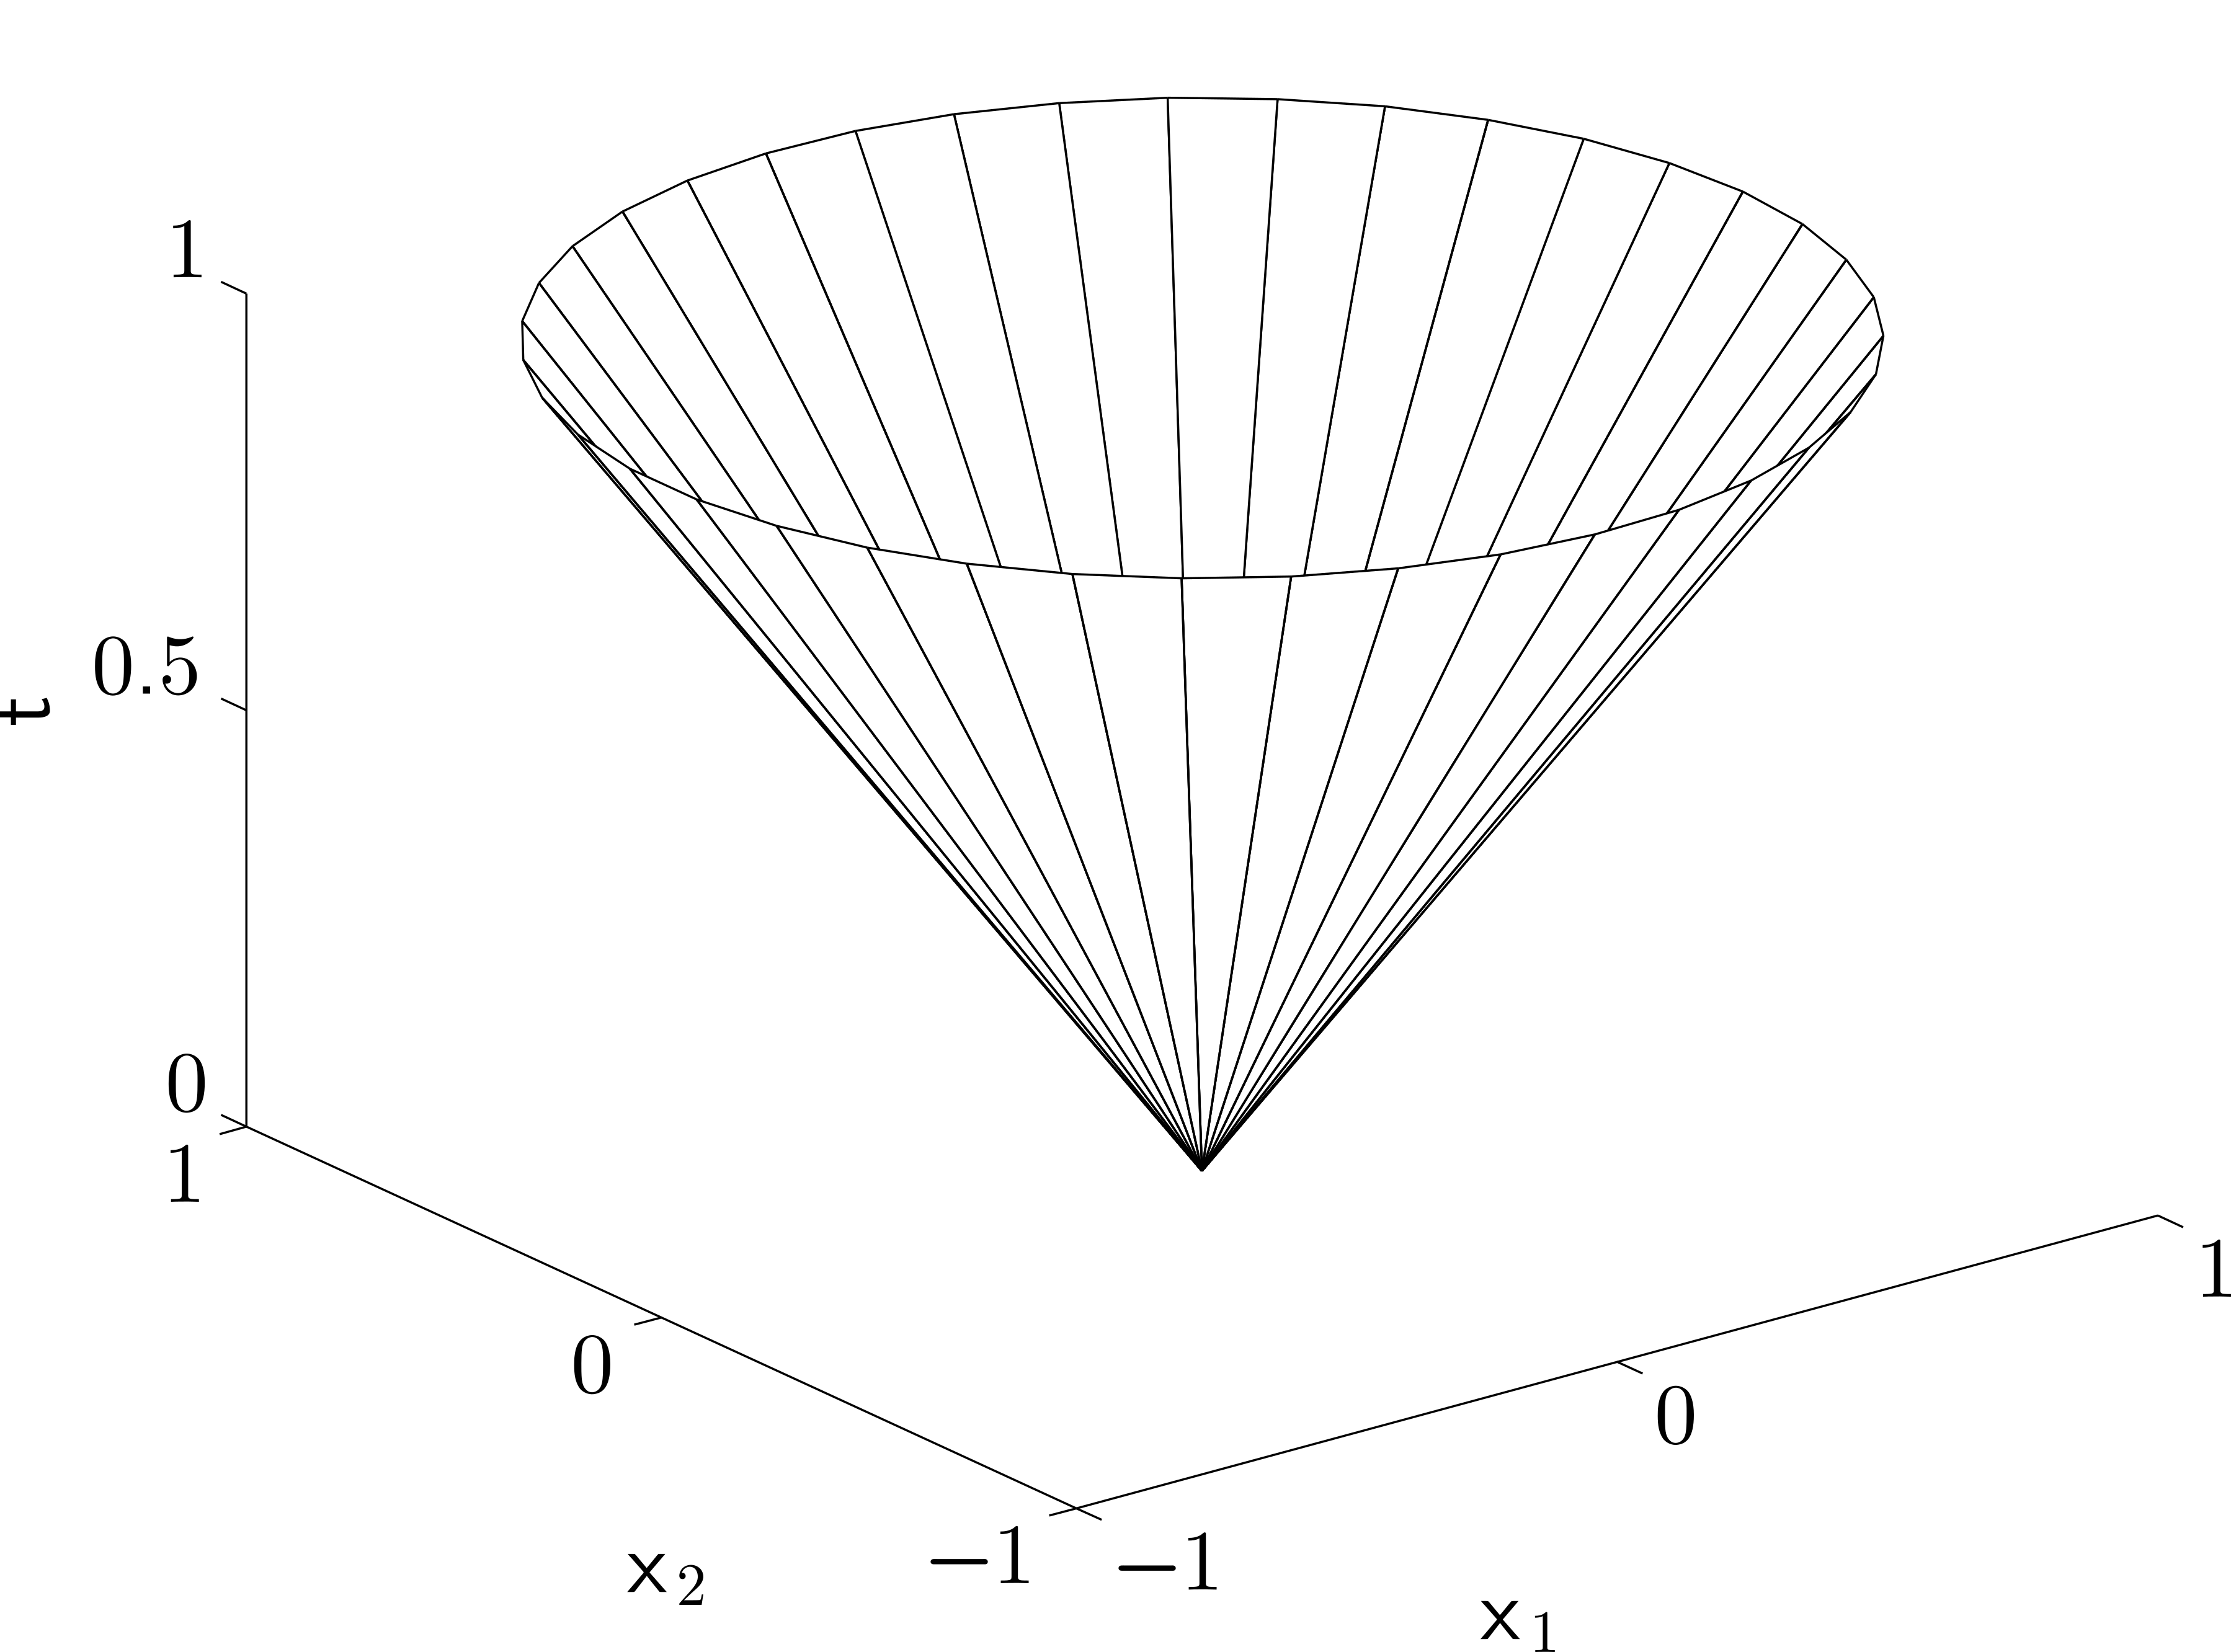
\includegraphics[width=.5\textwidth]{../Graphics/031.png}\hfil

\clearpage
\hfil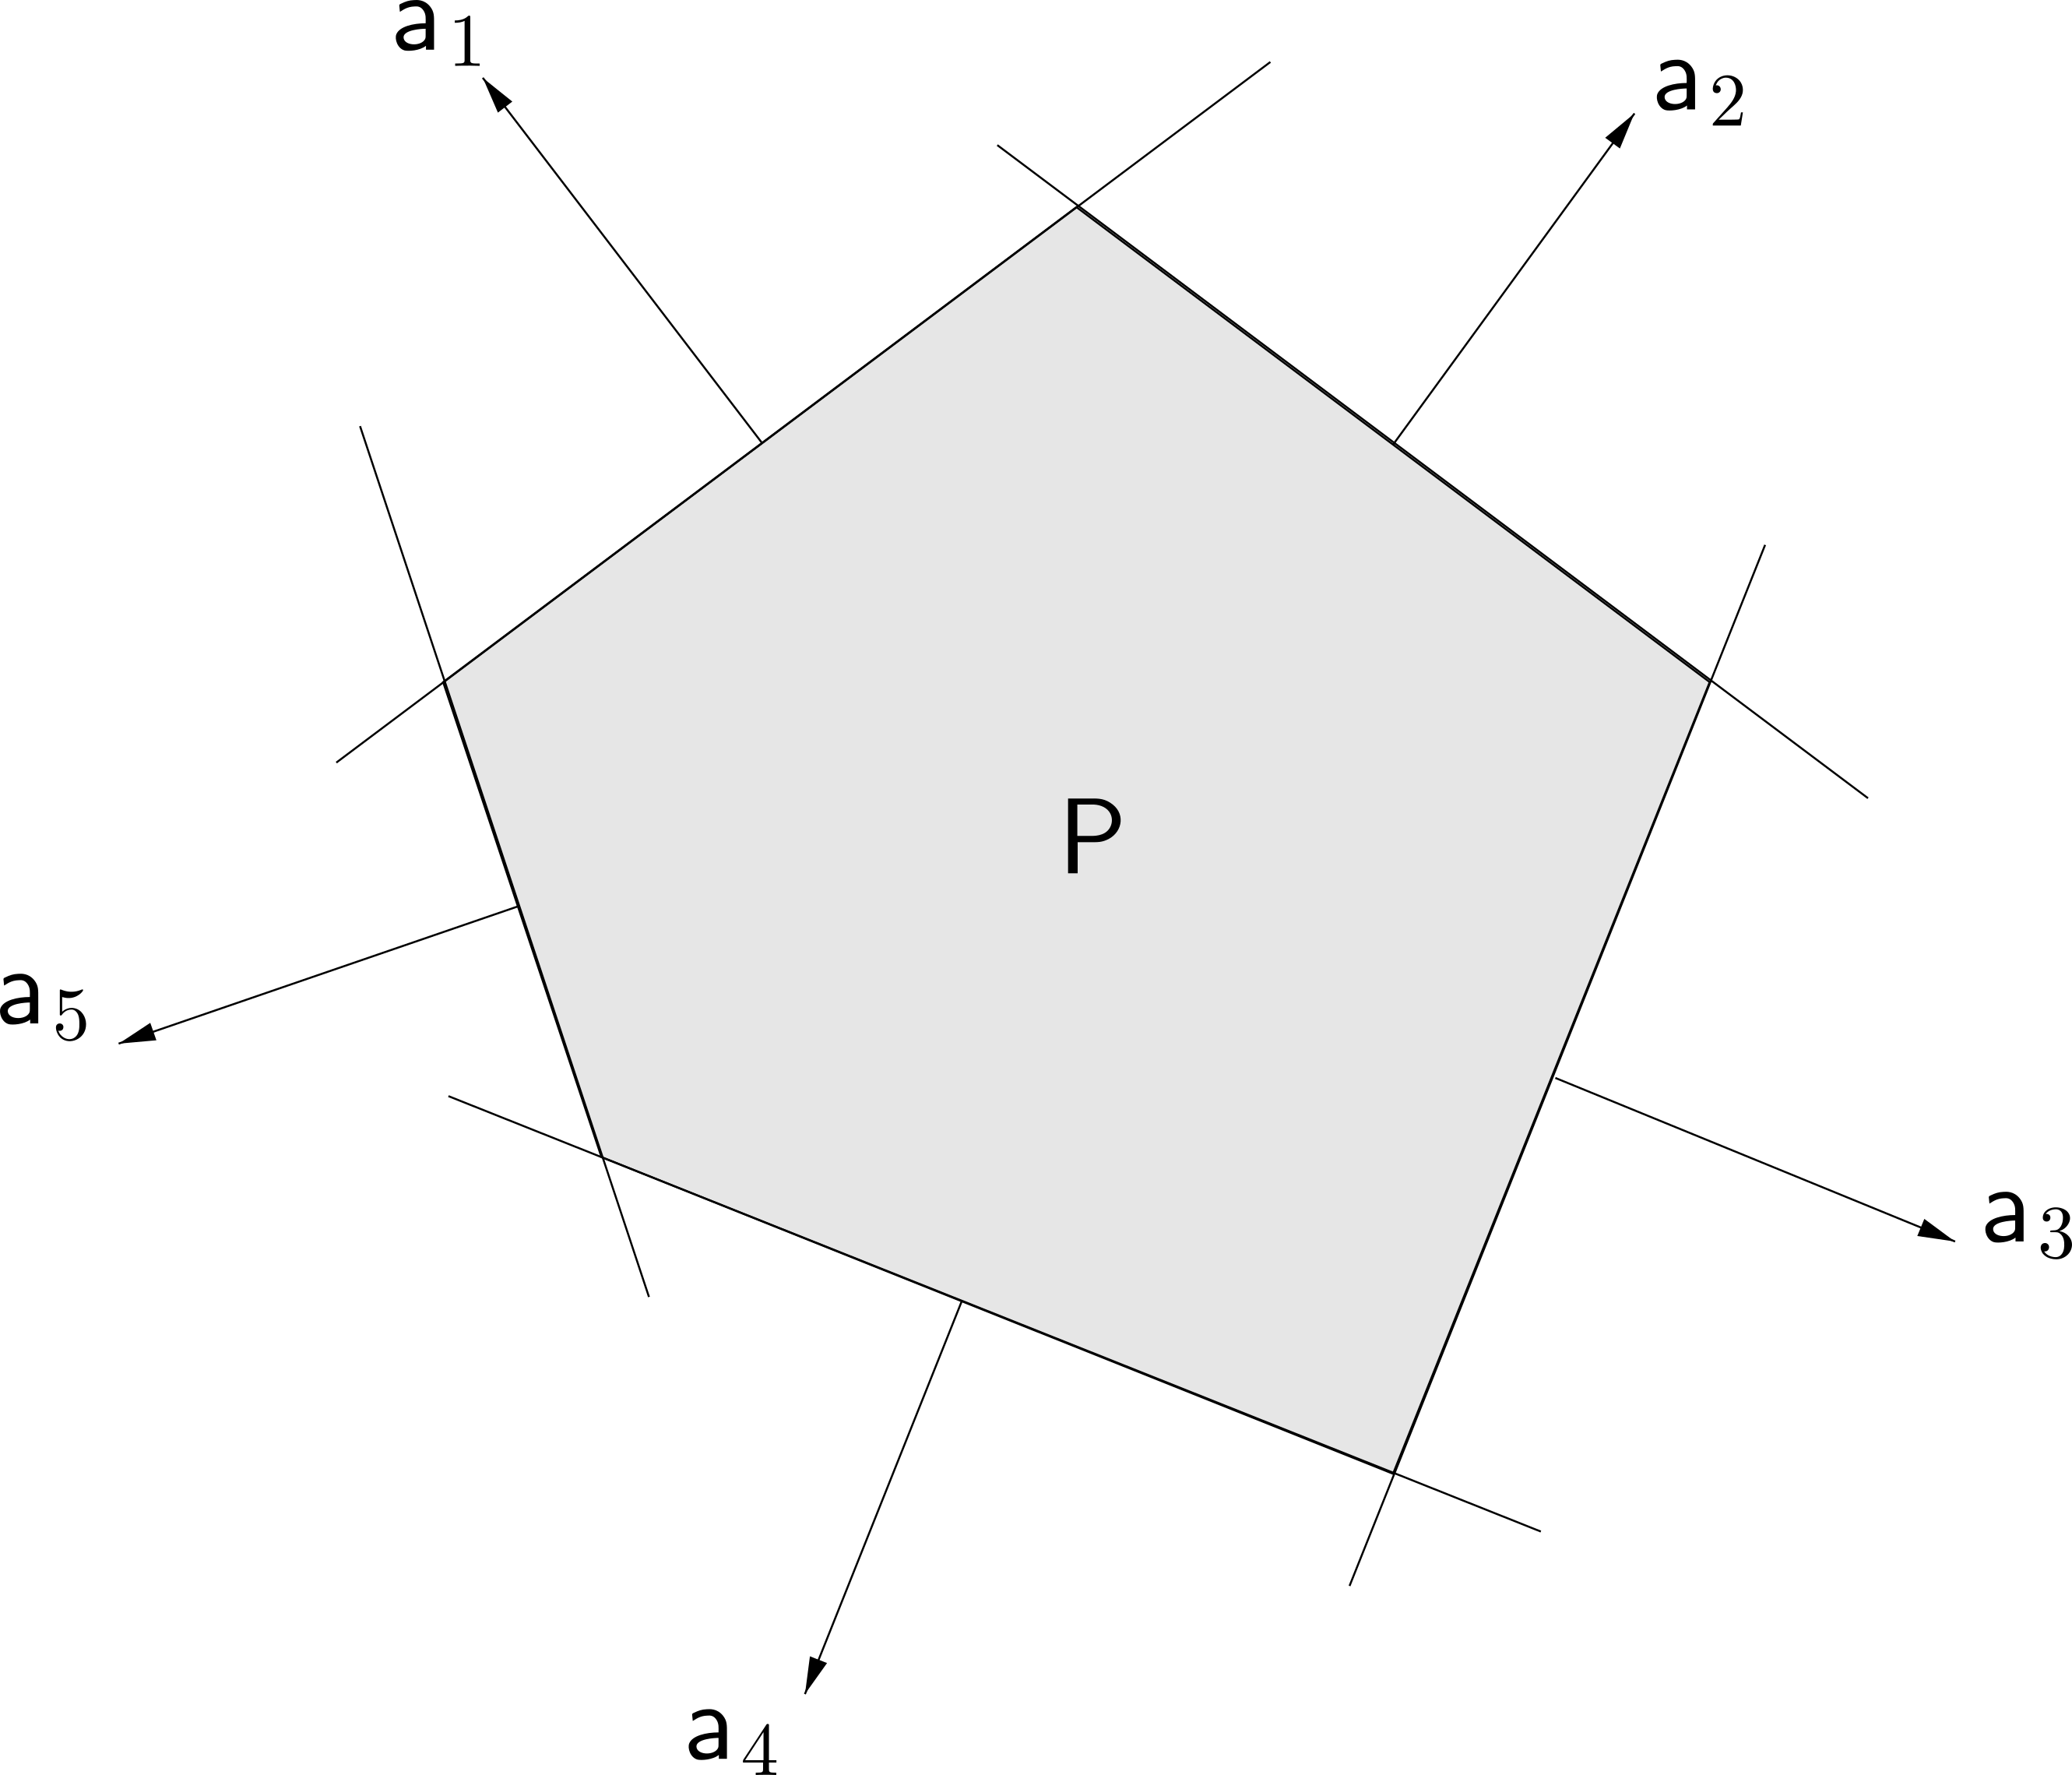
\includegraphics[width=.5\textwidth]{../Graphics/032.png}\hfil

\clearpage
\hfil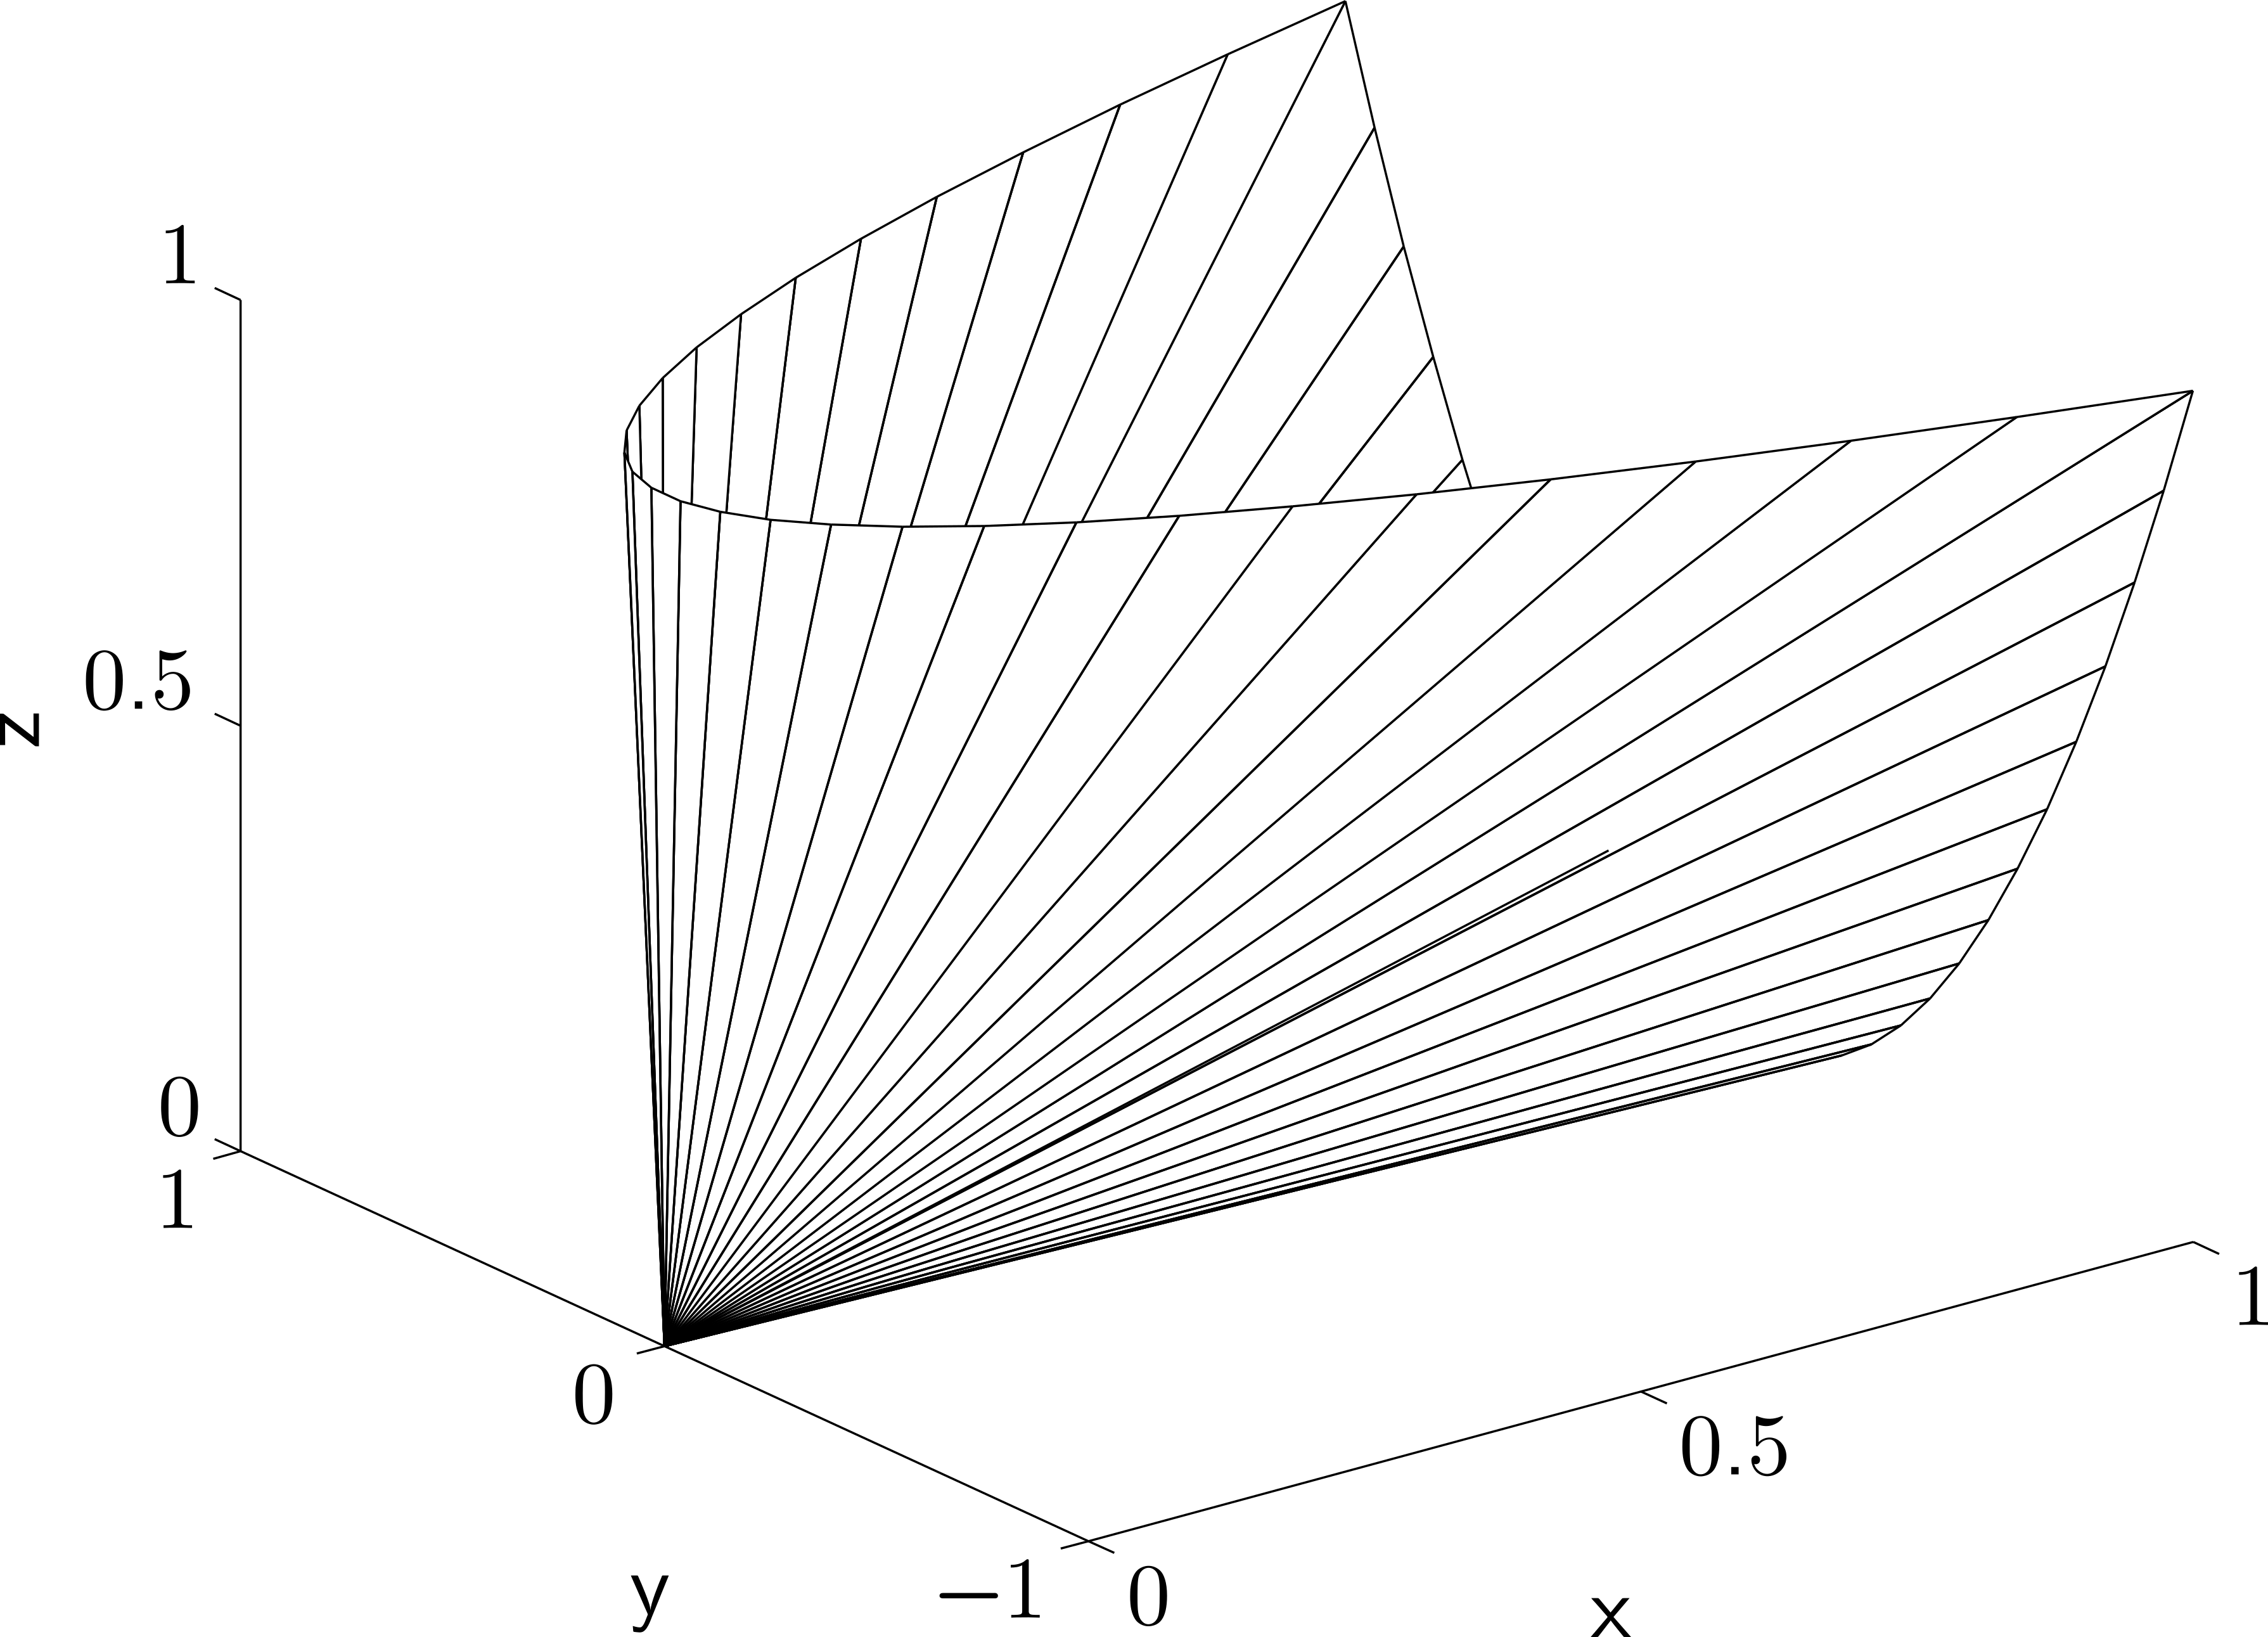
\includegraphics[width=.5\textwidth]{../Graphics/035.png}\hfil

\clearpage
\hfil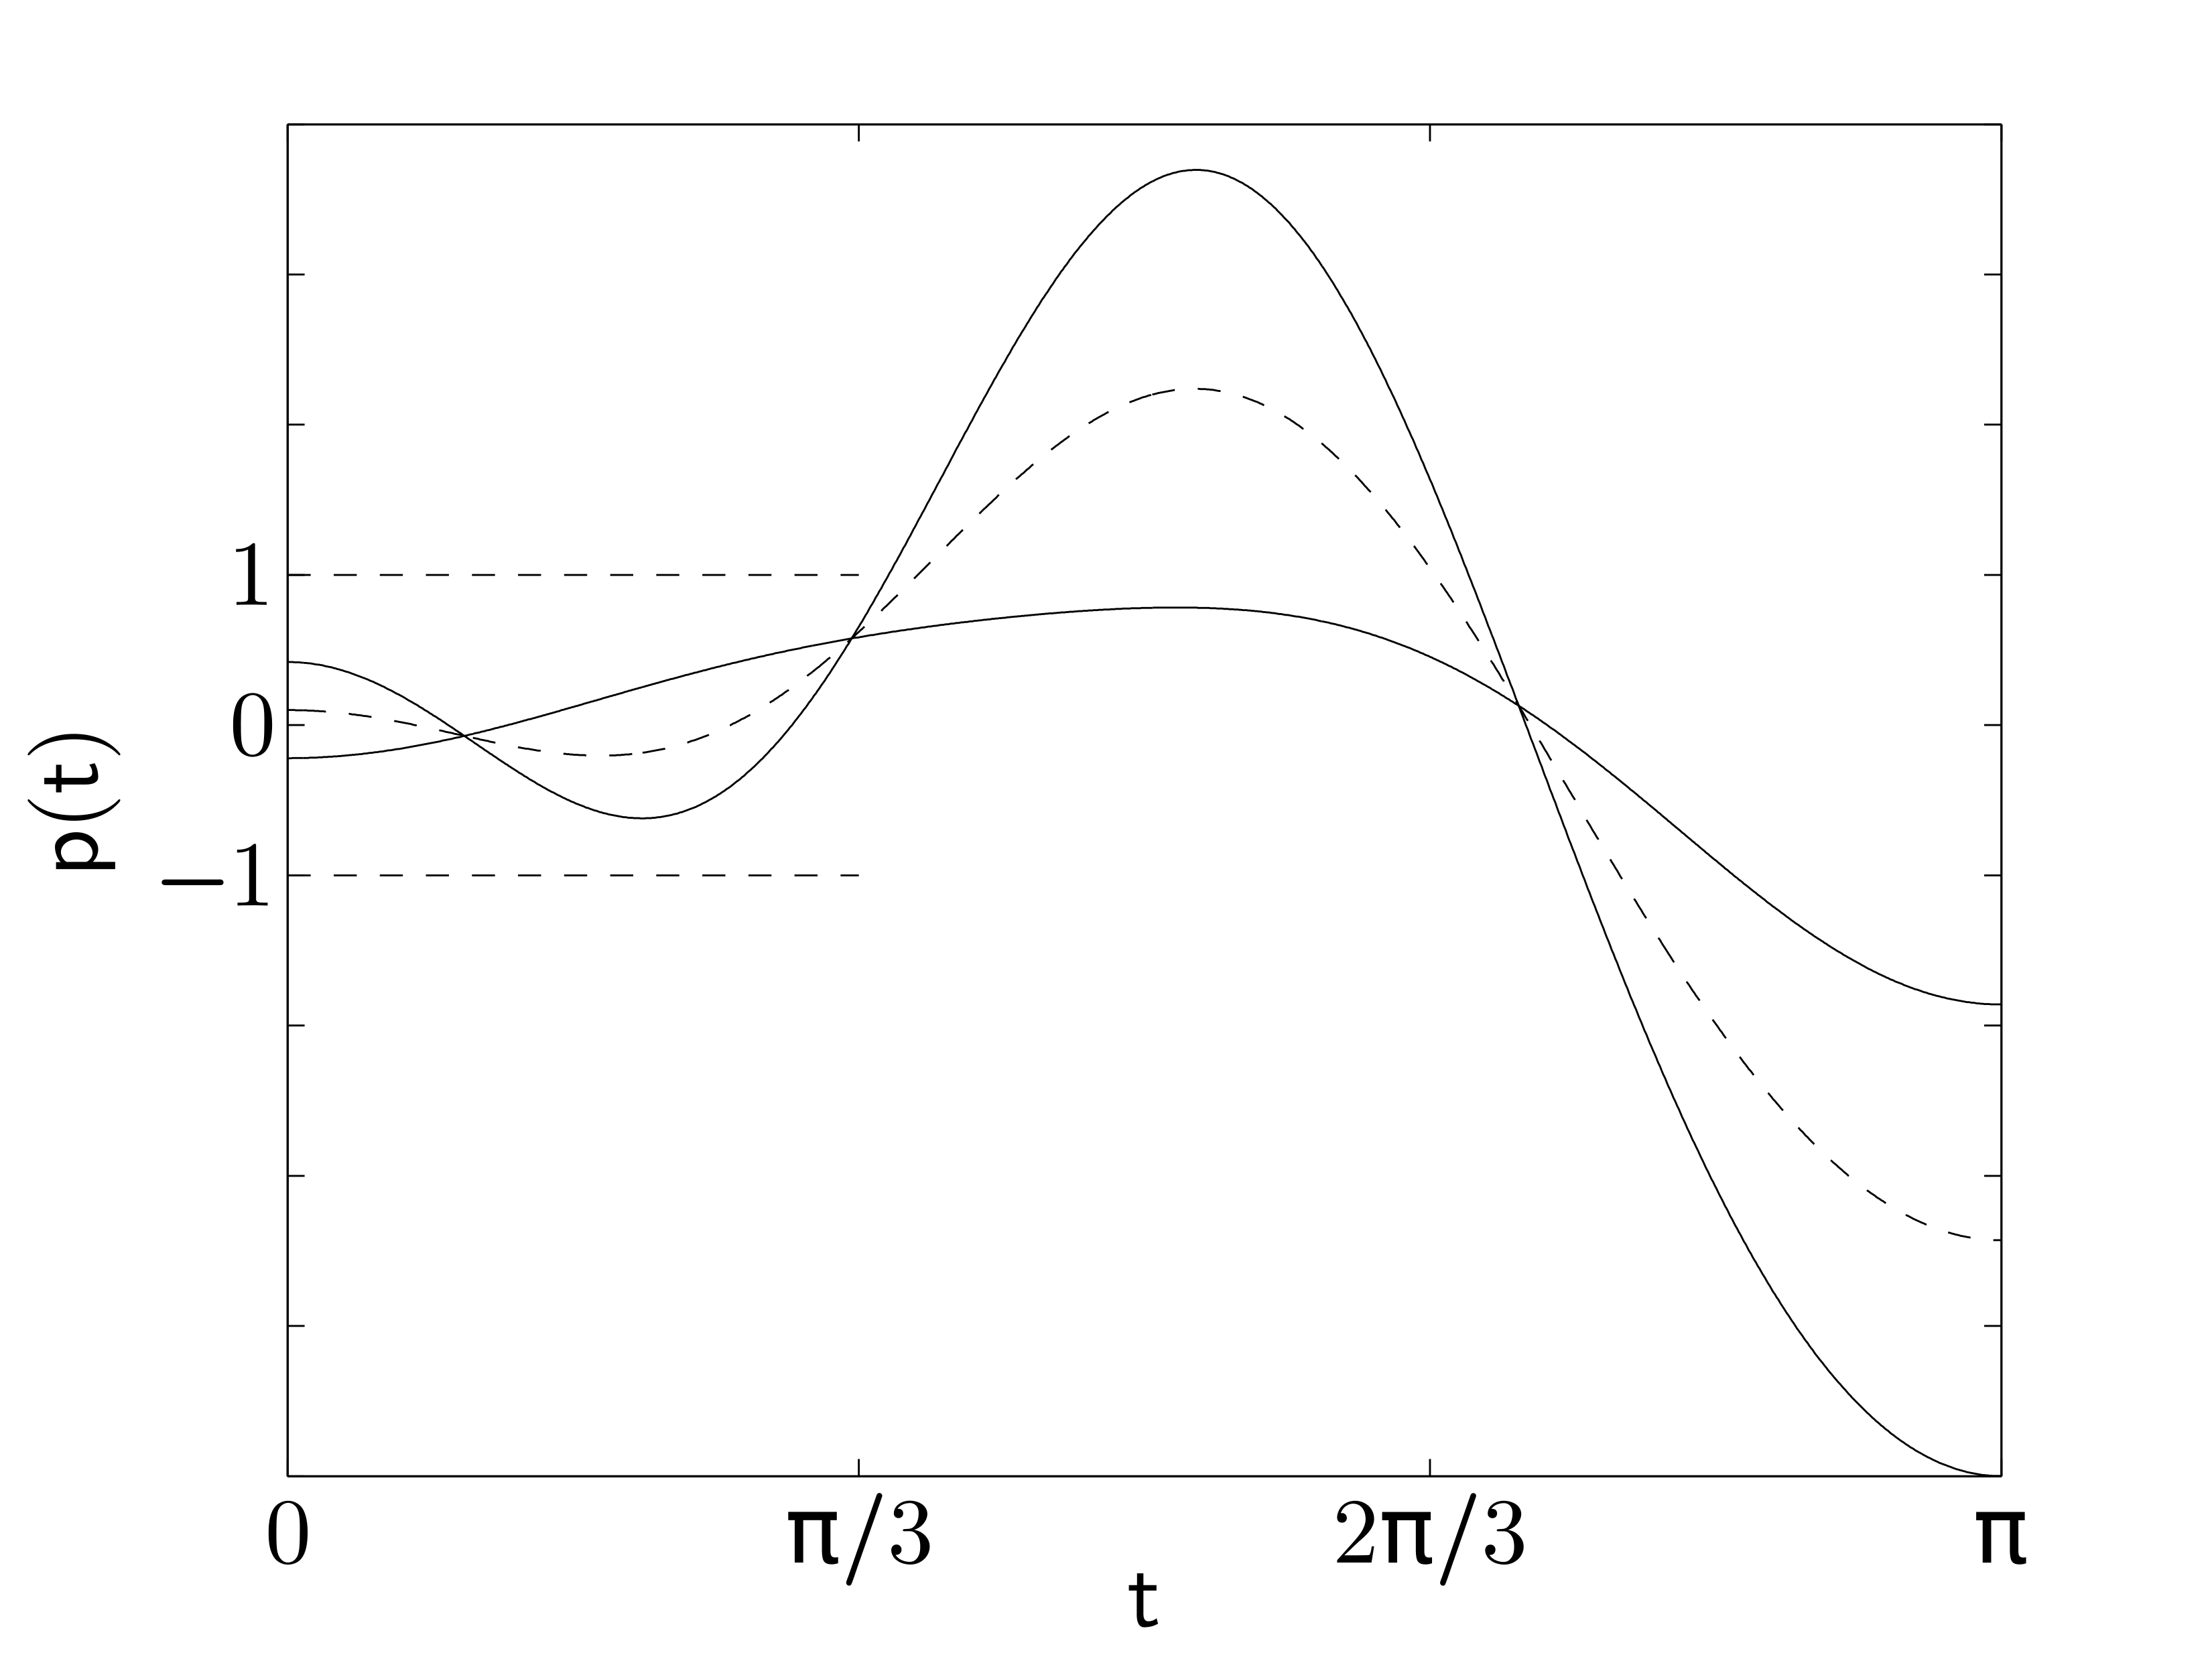
\includegraphics[width=.5\textwidth]{../Graphics/037a.png}\hfil

\clearpage
\hfil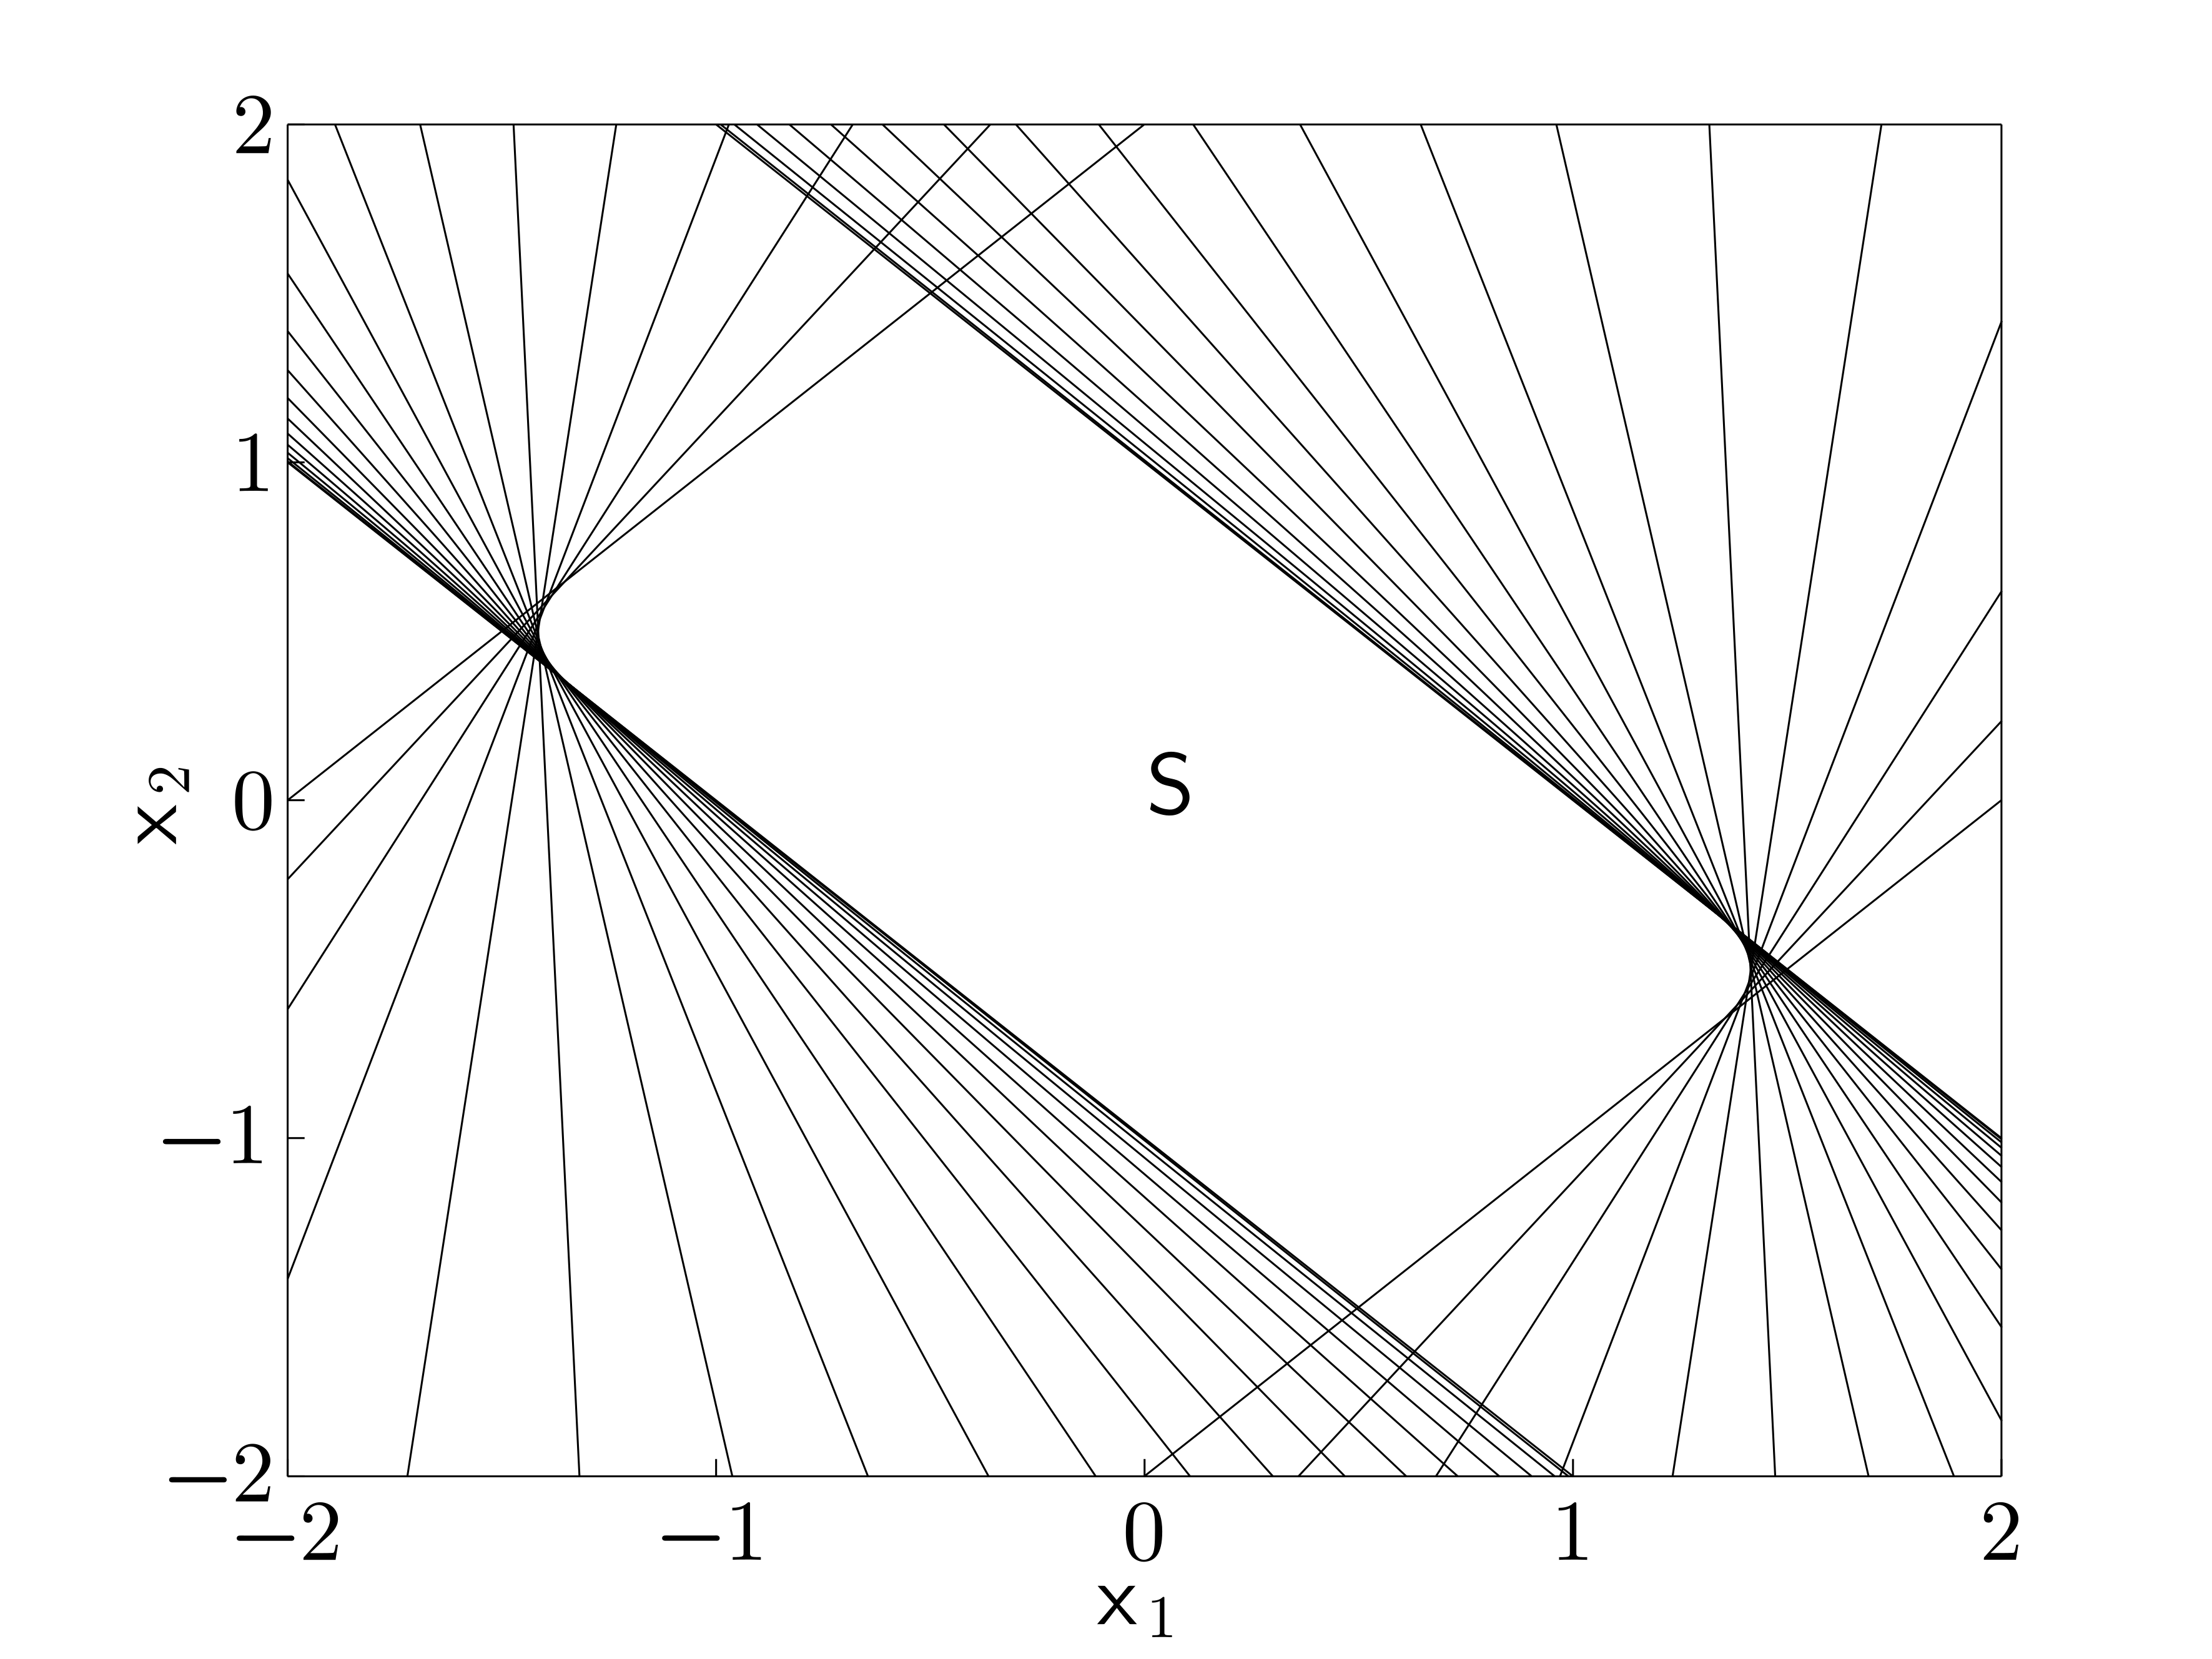
\includegraphics[width=.5\textwidth]{../Graphics/037b.png}\hfil

\clearpage
\hfil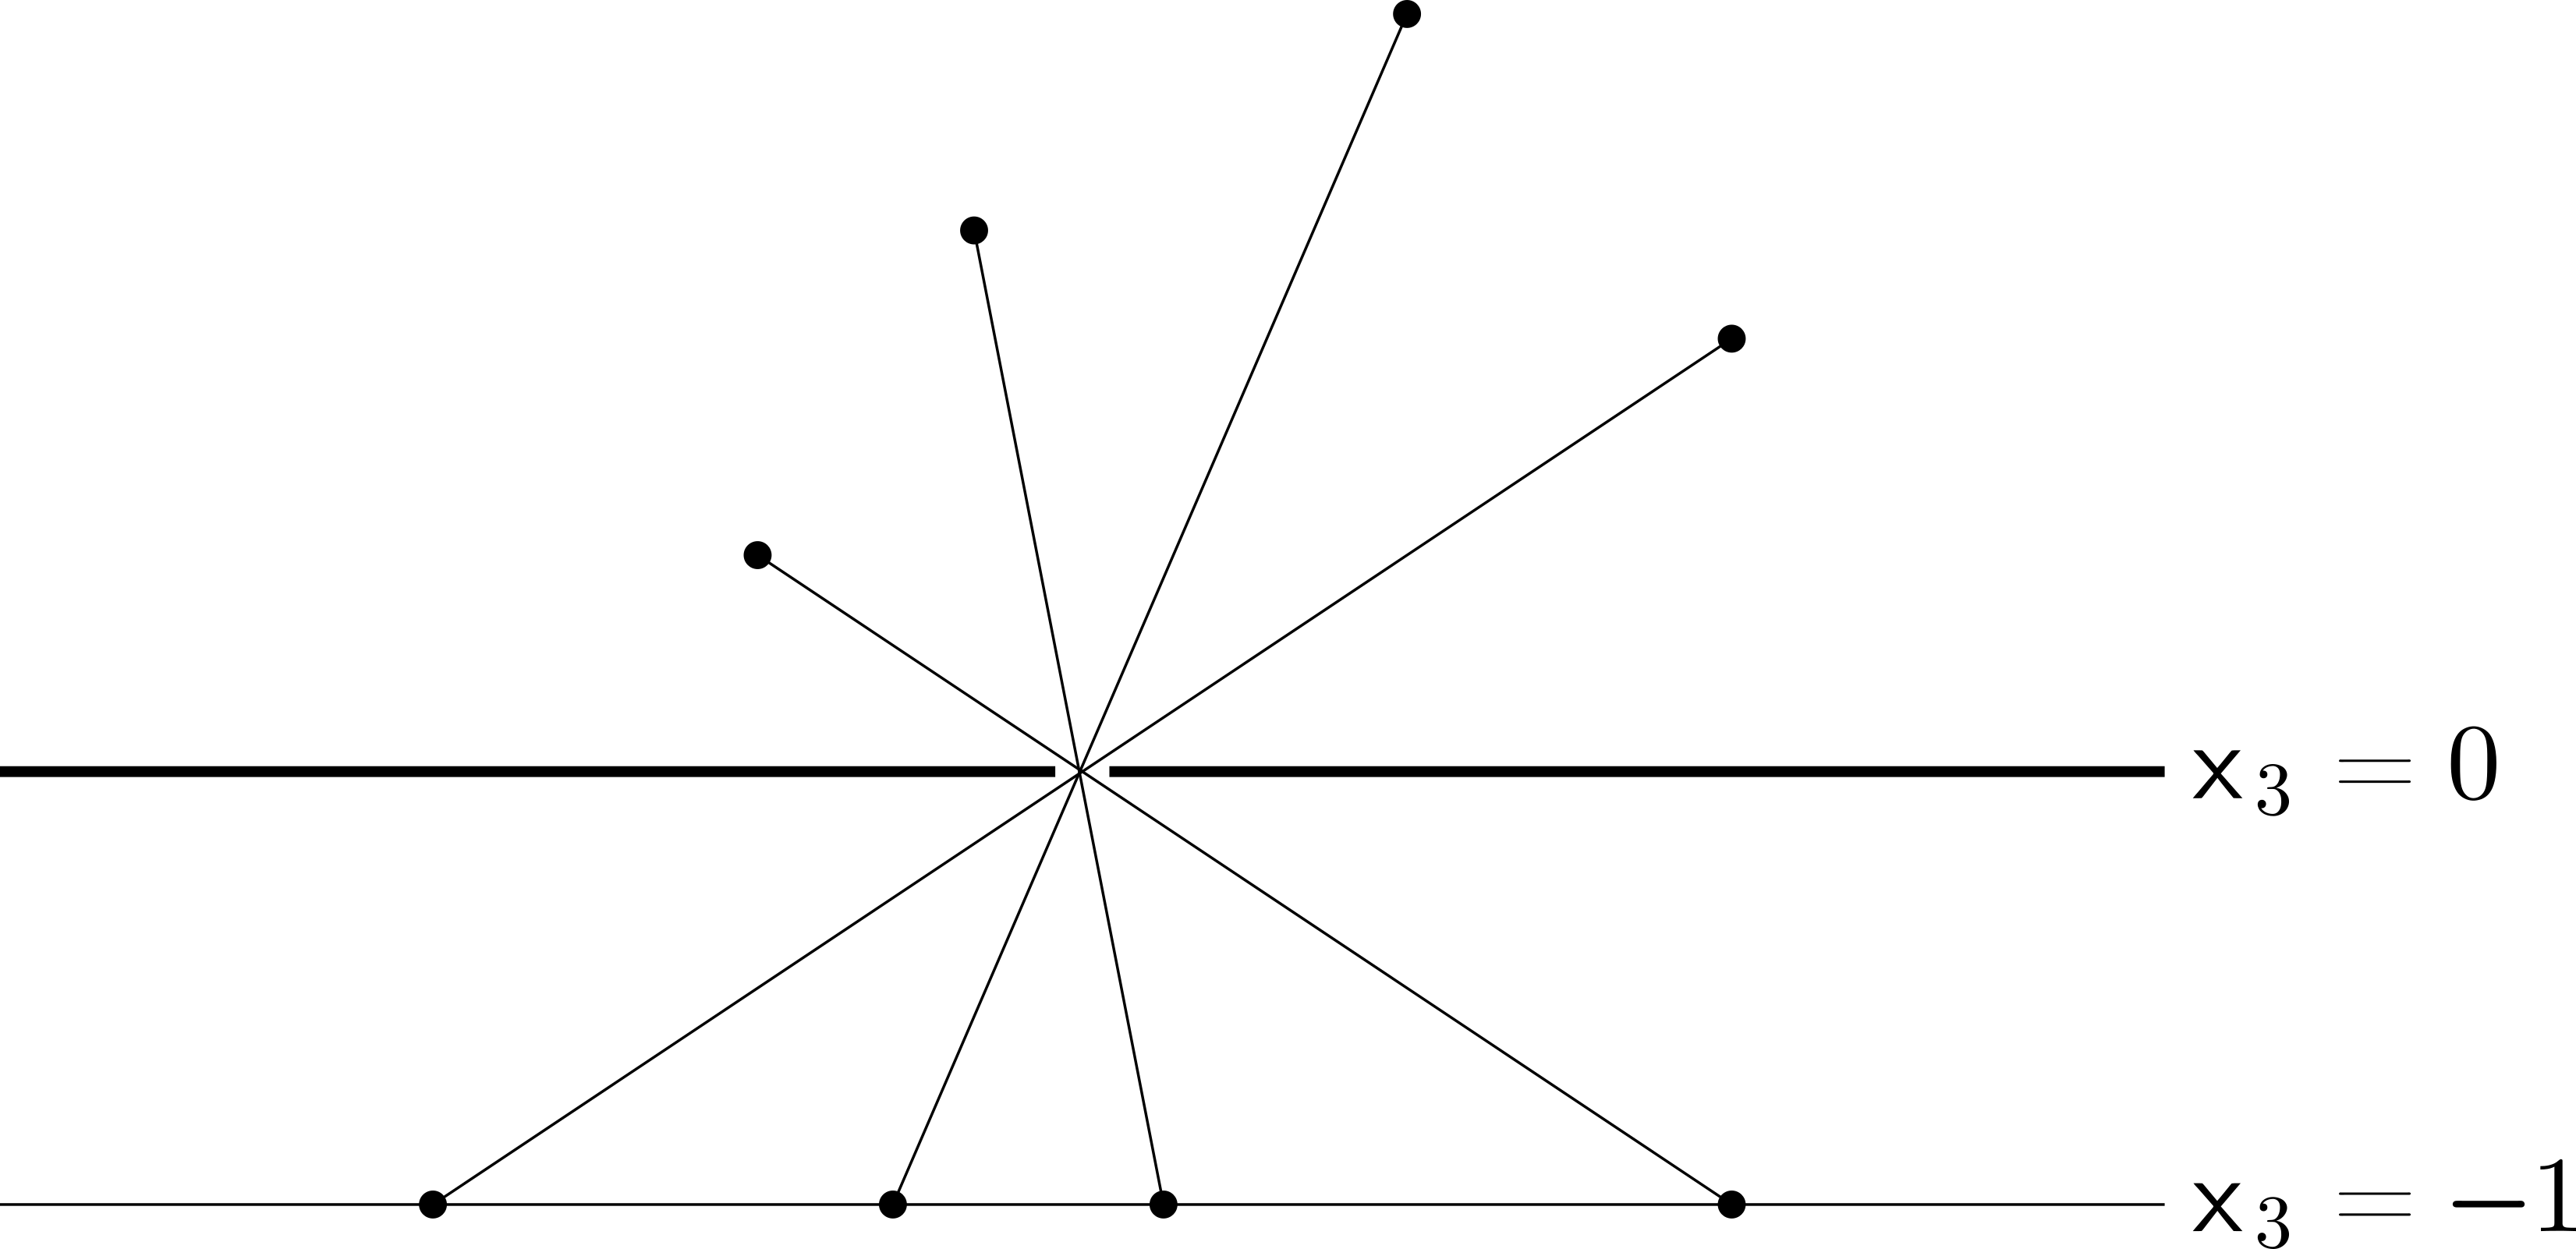
\includegraphics[width=.5\textwidth]{../Graphics/040.png}\hfil

\clearpage
\hfil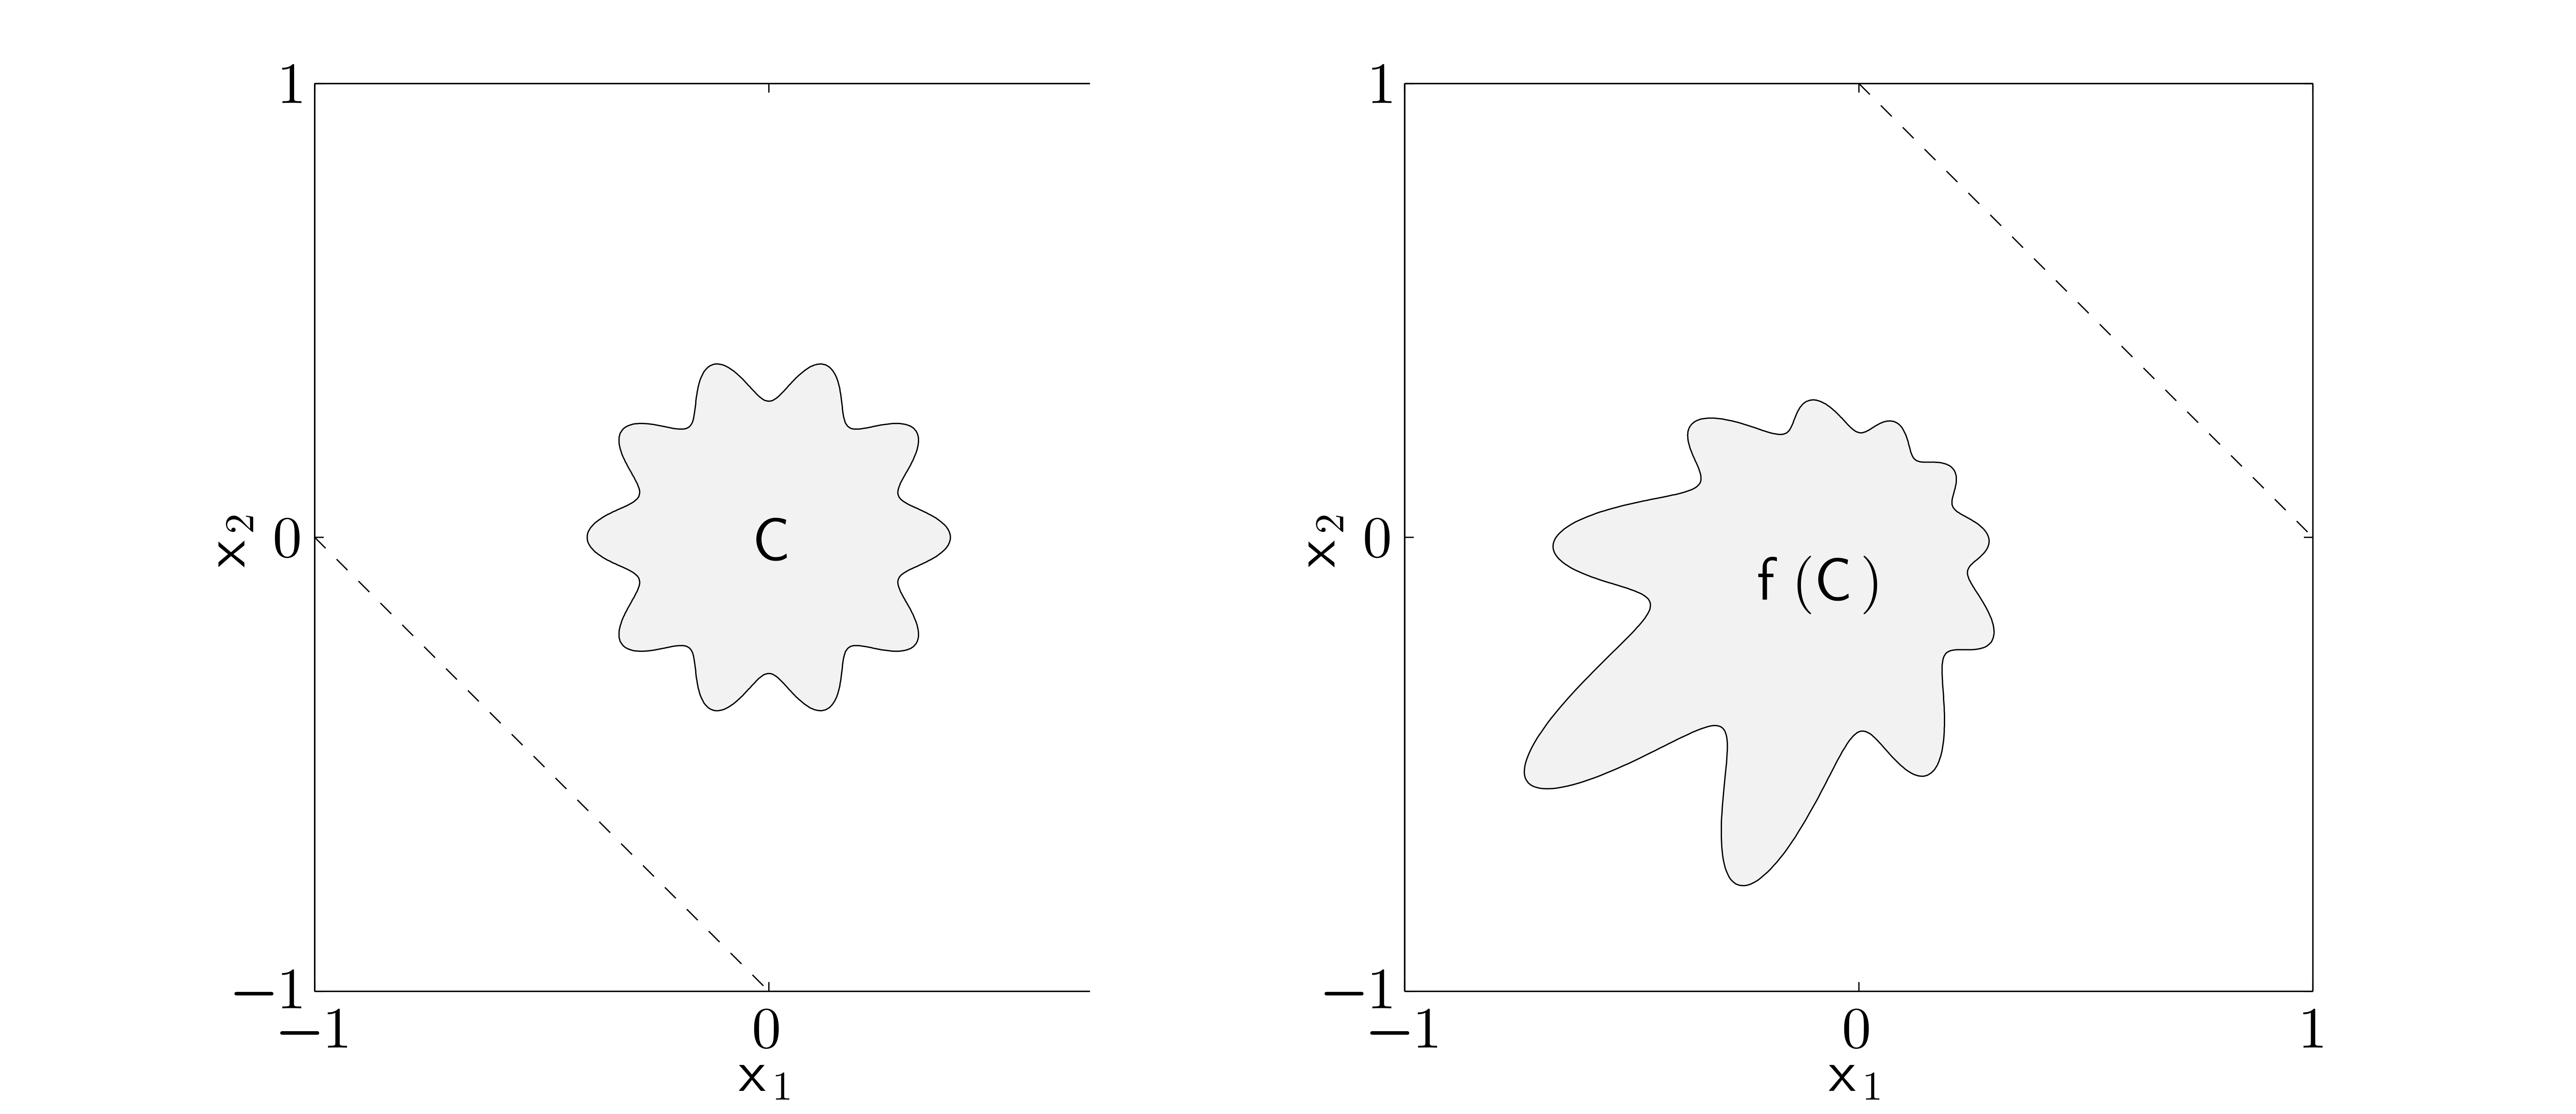
\includegraphics[width=.5\textwidth]{../Graphics/042.png}\hfil

\clearpage
\hfil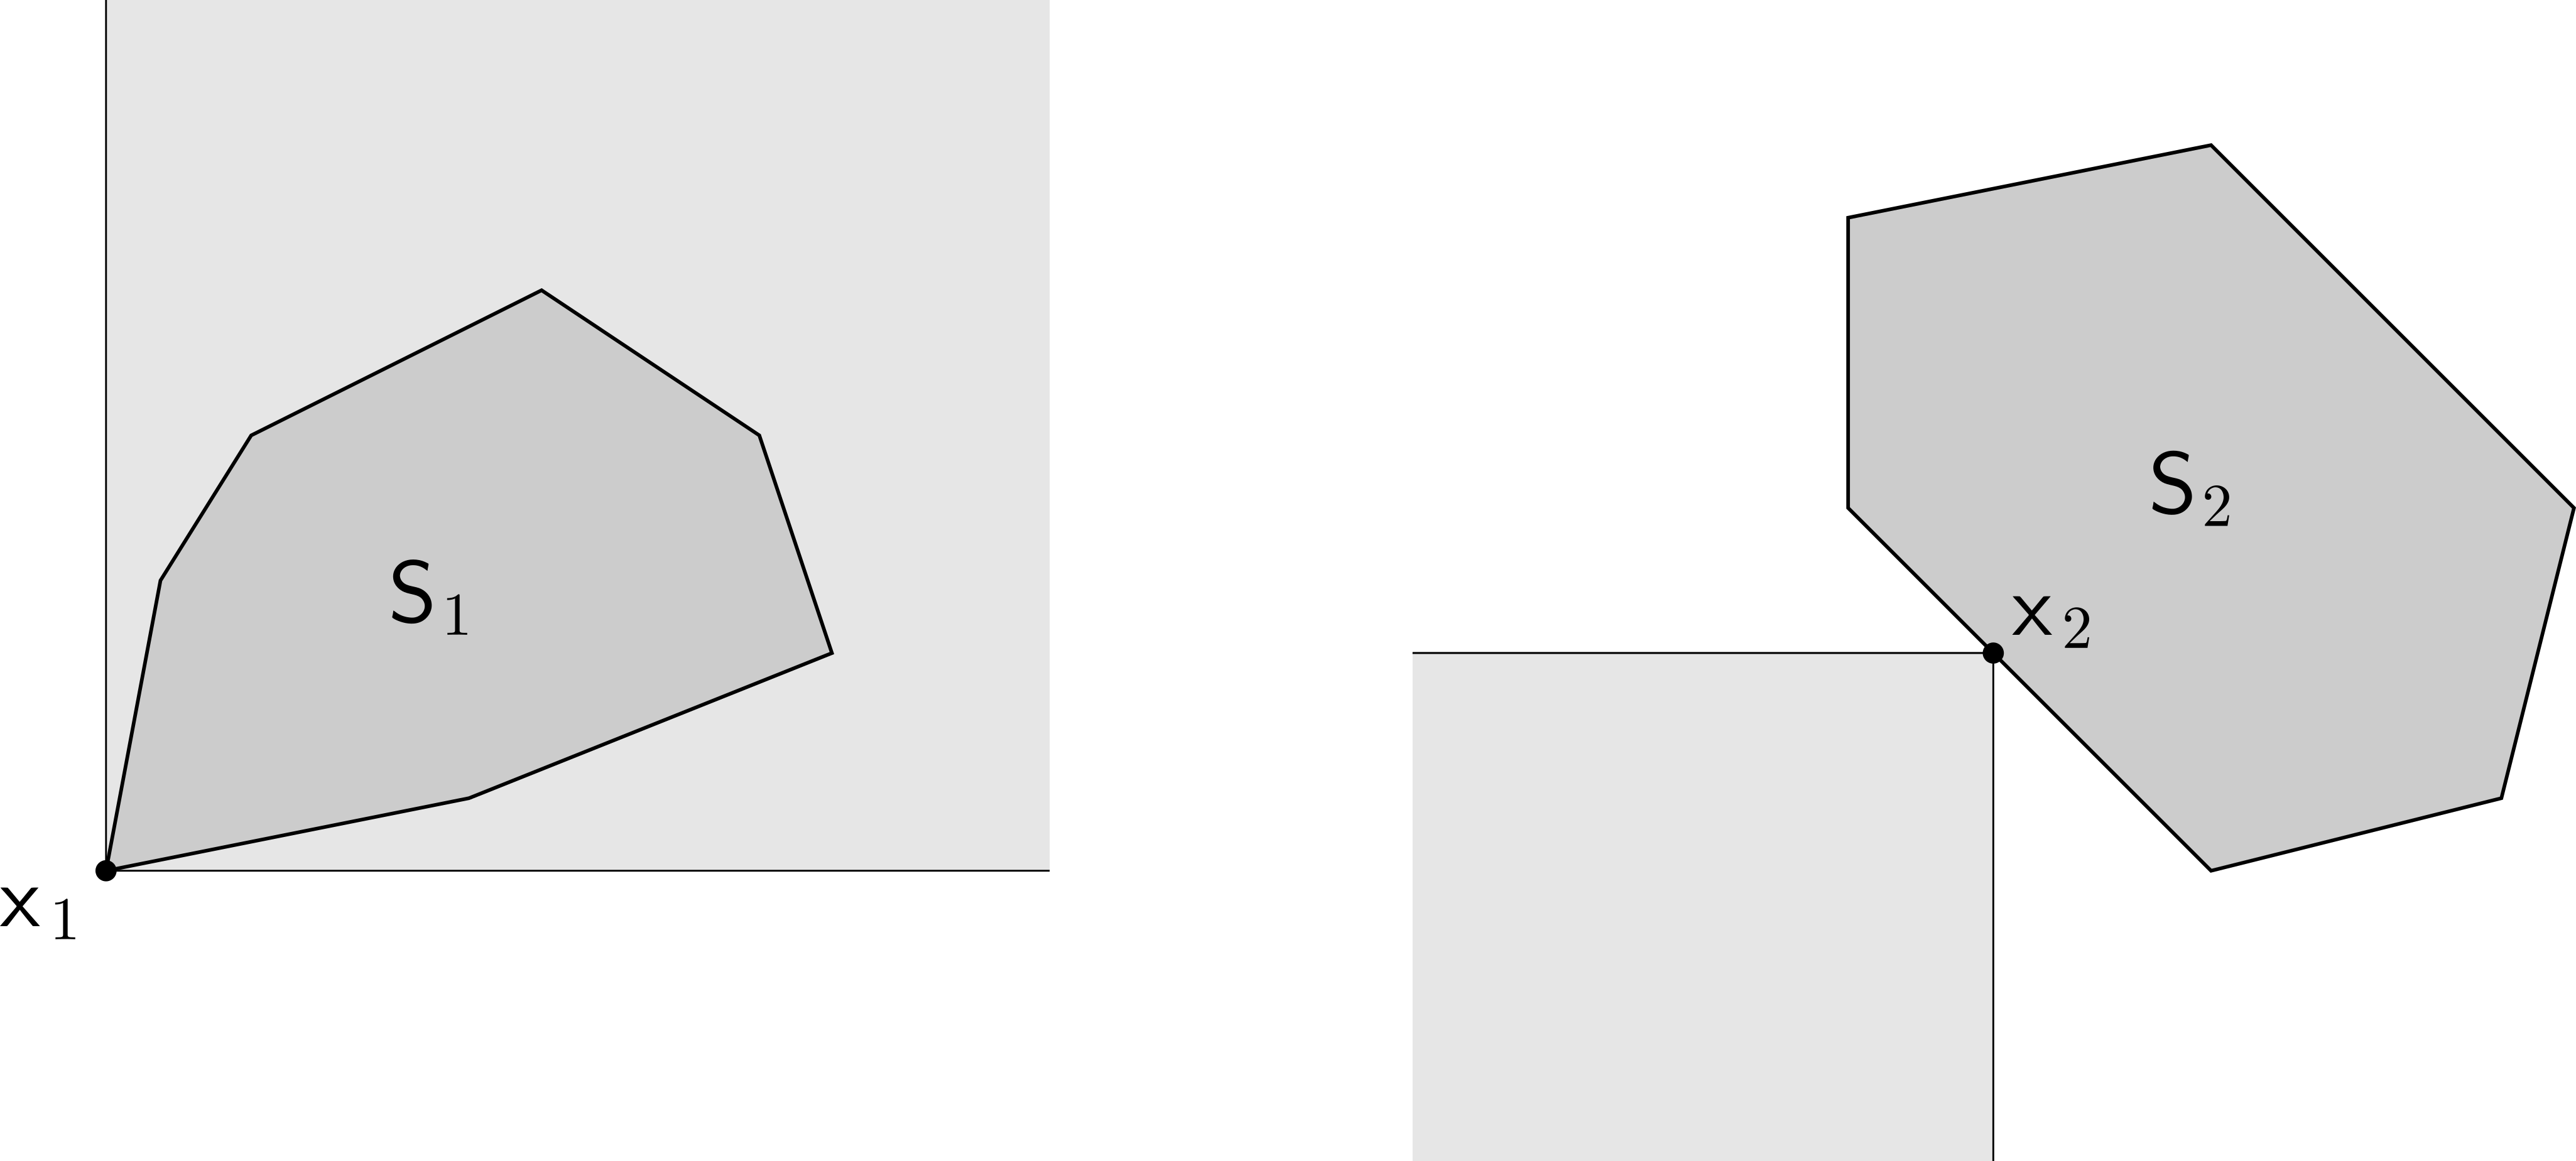
\includegraphics[width=.5\textwidth]{../Graphics/046.png}\hfil

\clearpage
\hfil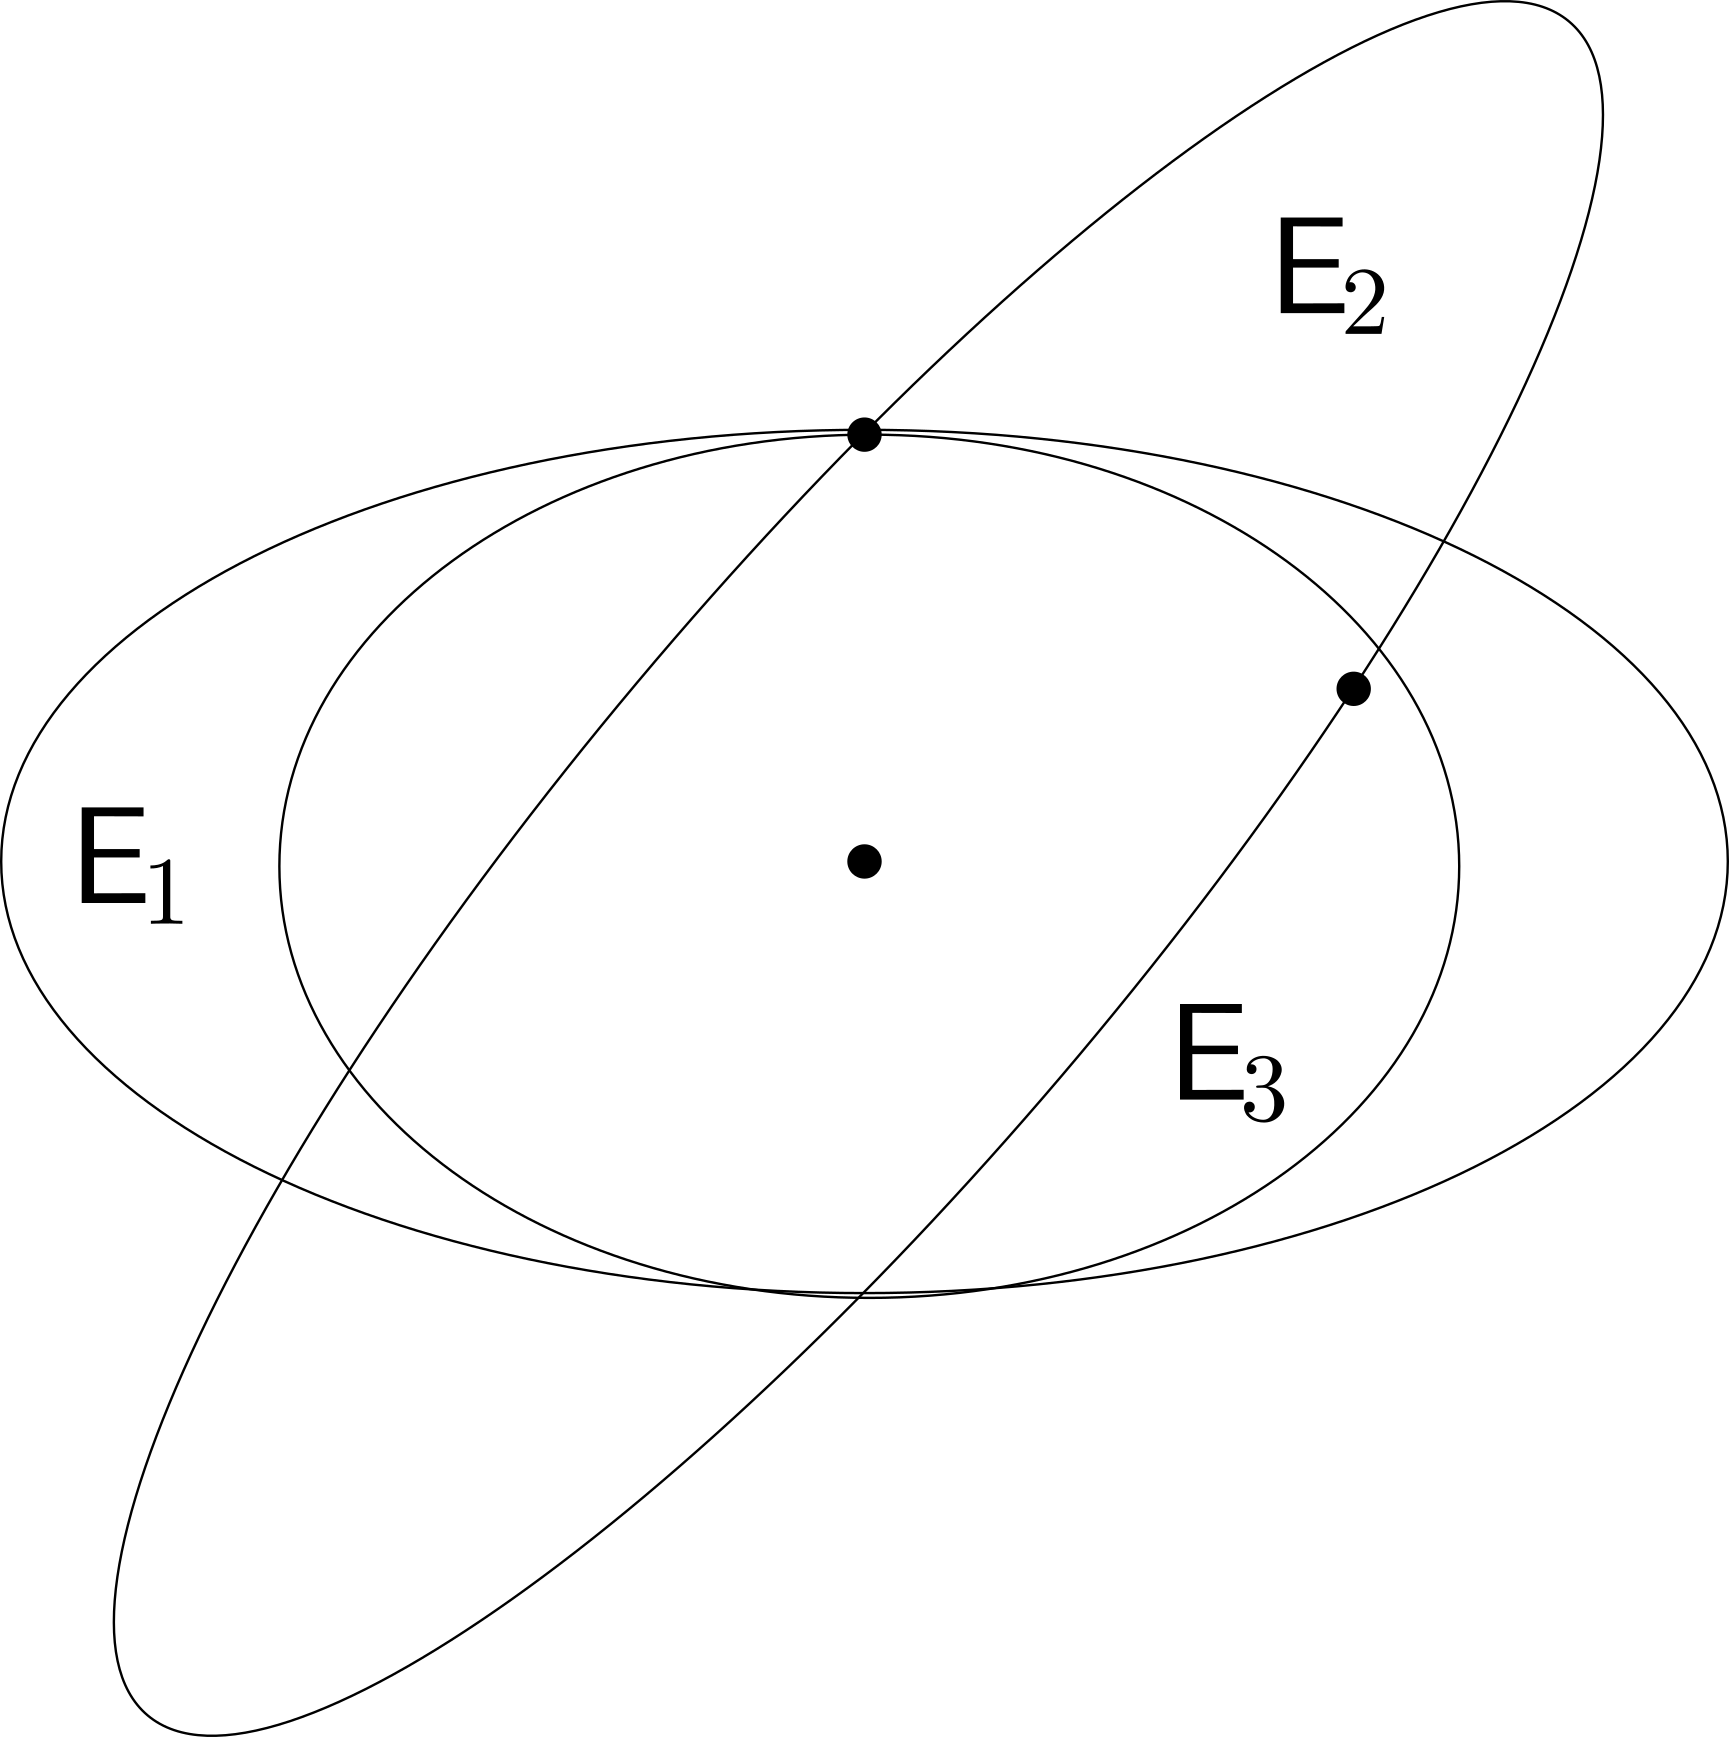
\includegraphics[width=.5\textwidth]{../Graphics/047a.png}\hfil

\clearpage
\hfil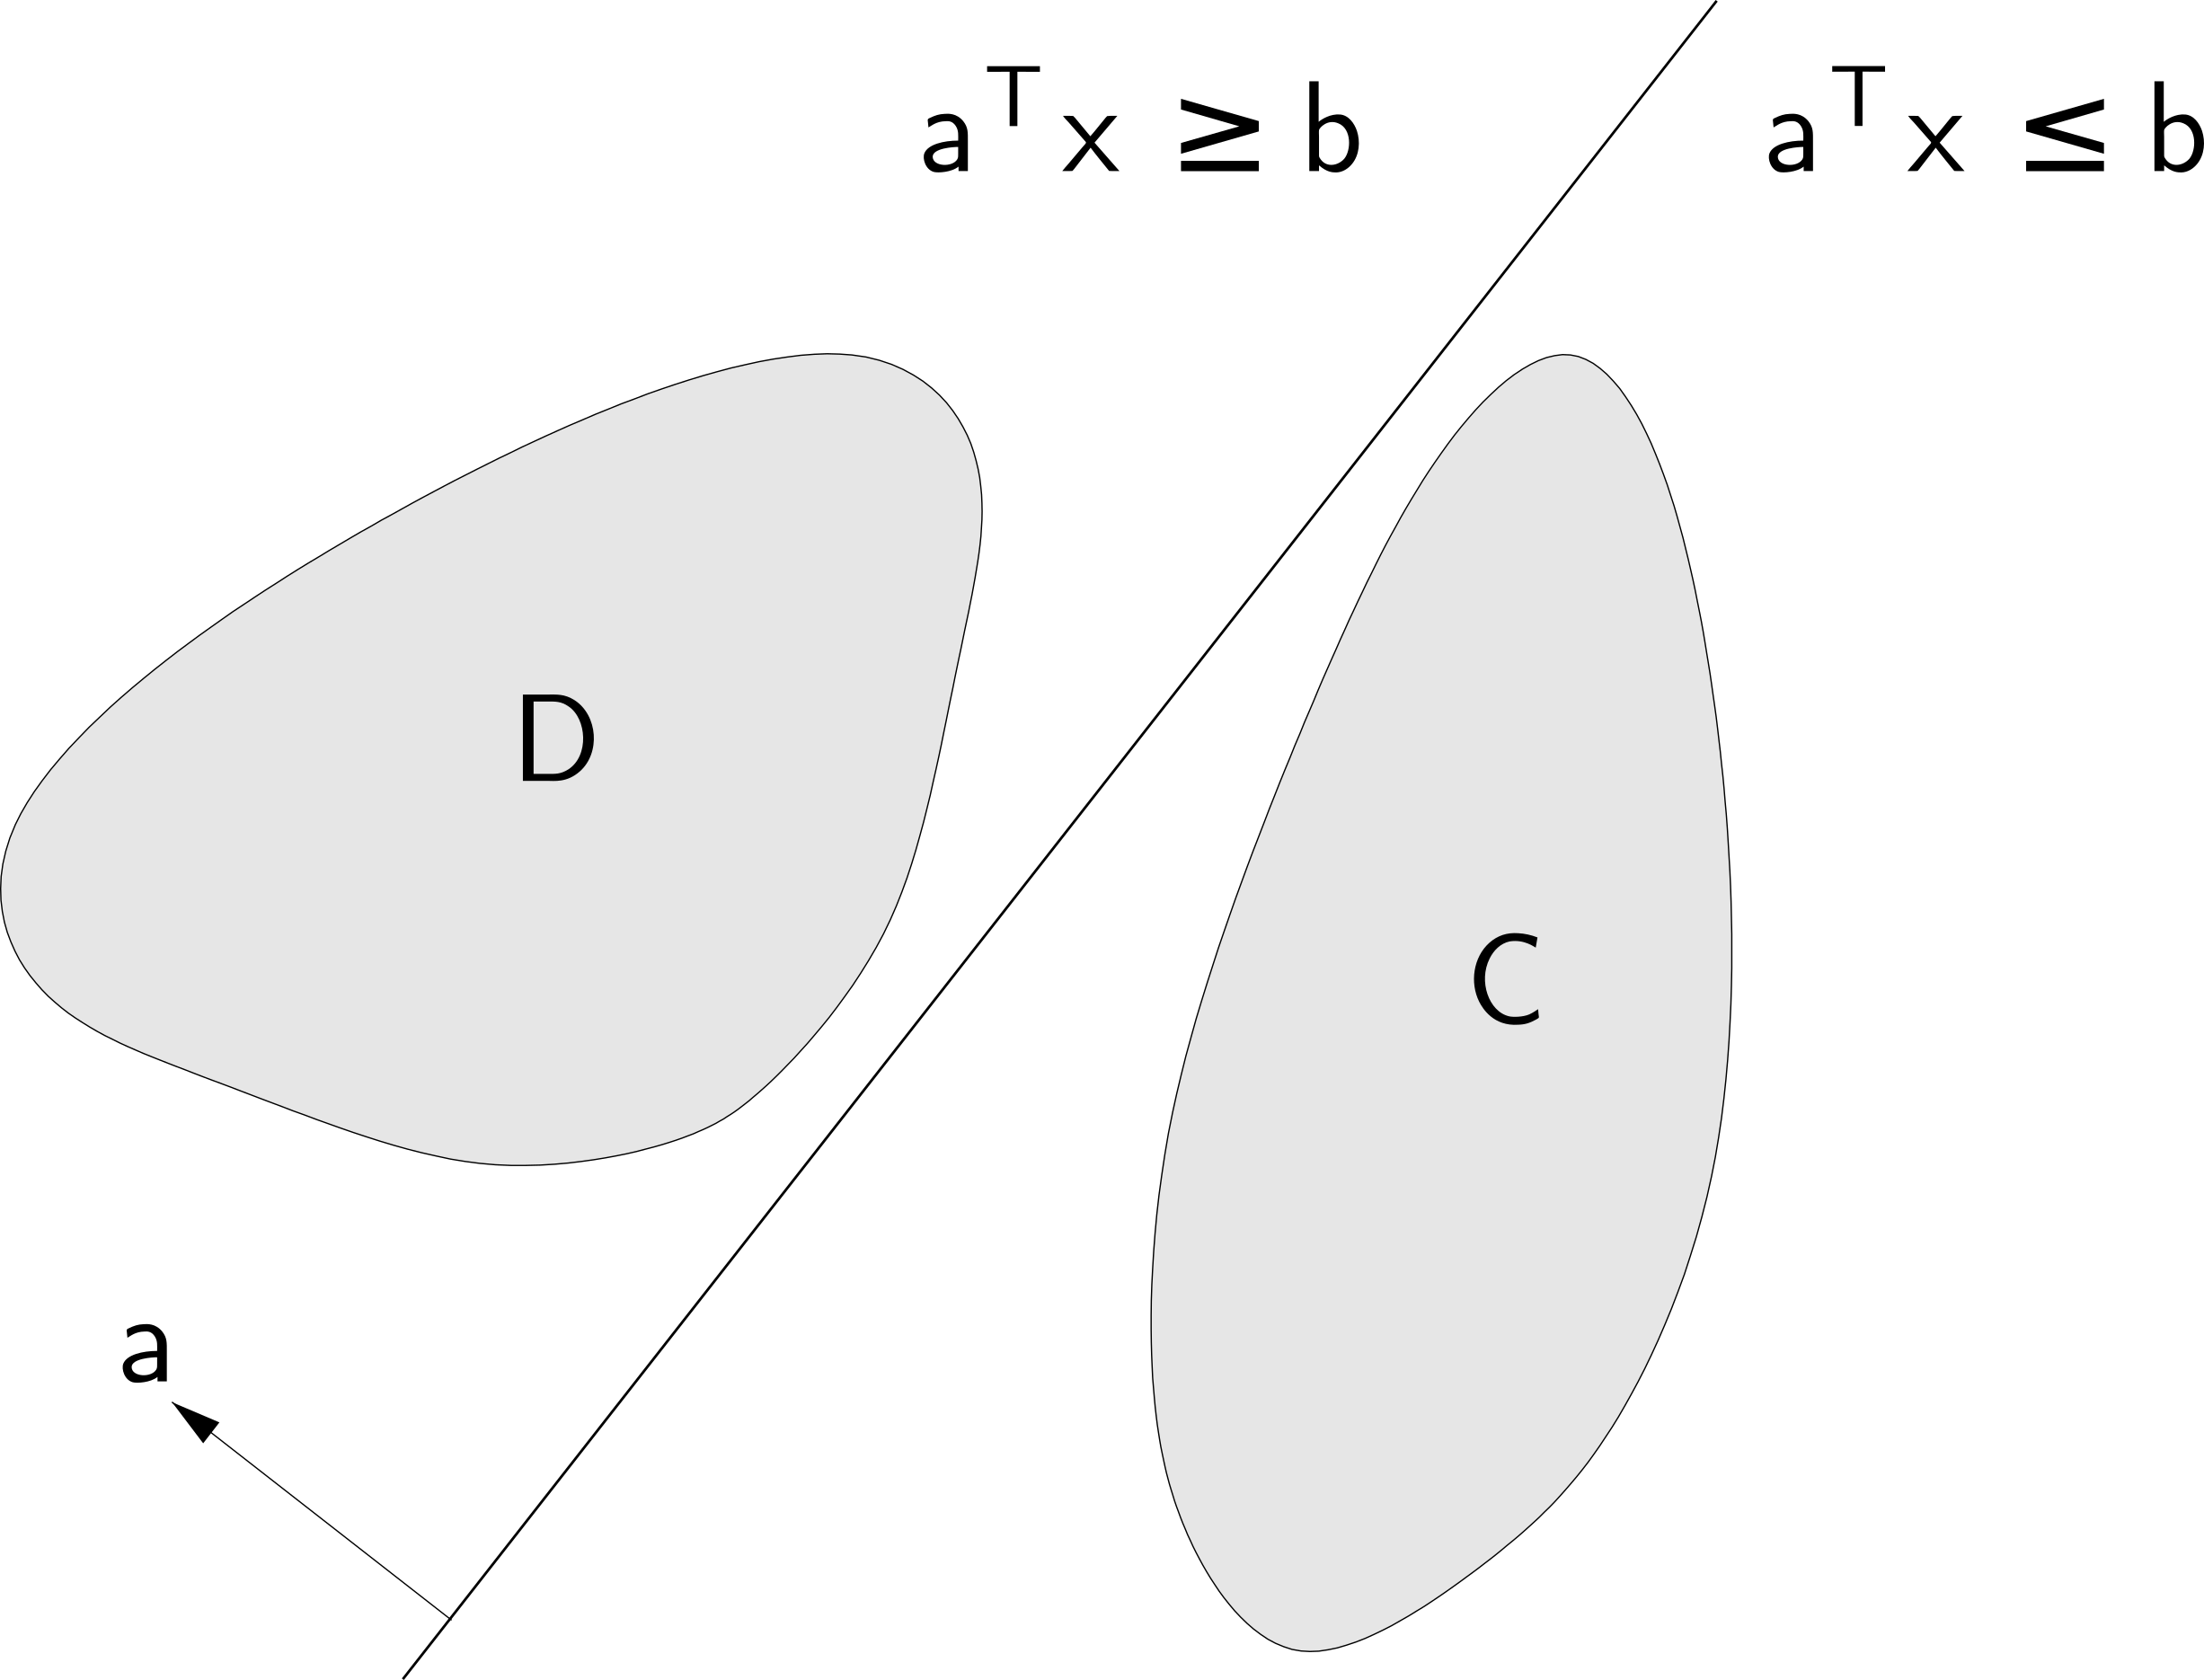
\includegraphics[width=.5\textwidth]{../Graphics/047b.png}\hfil

\clearpage
\hfil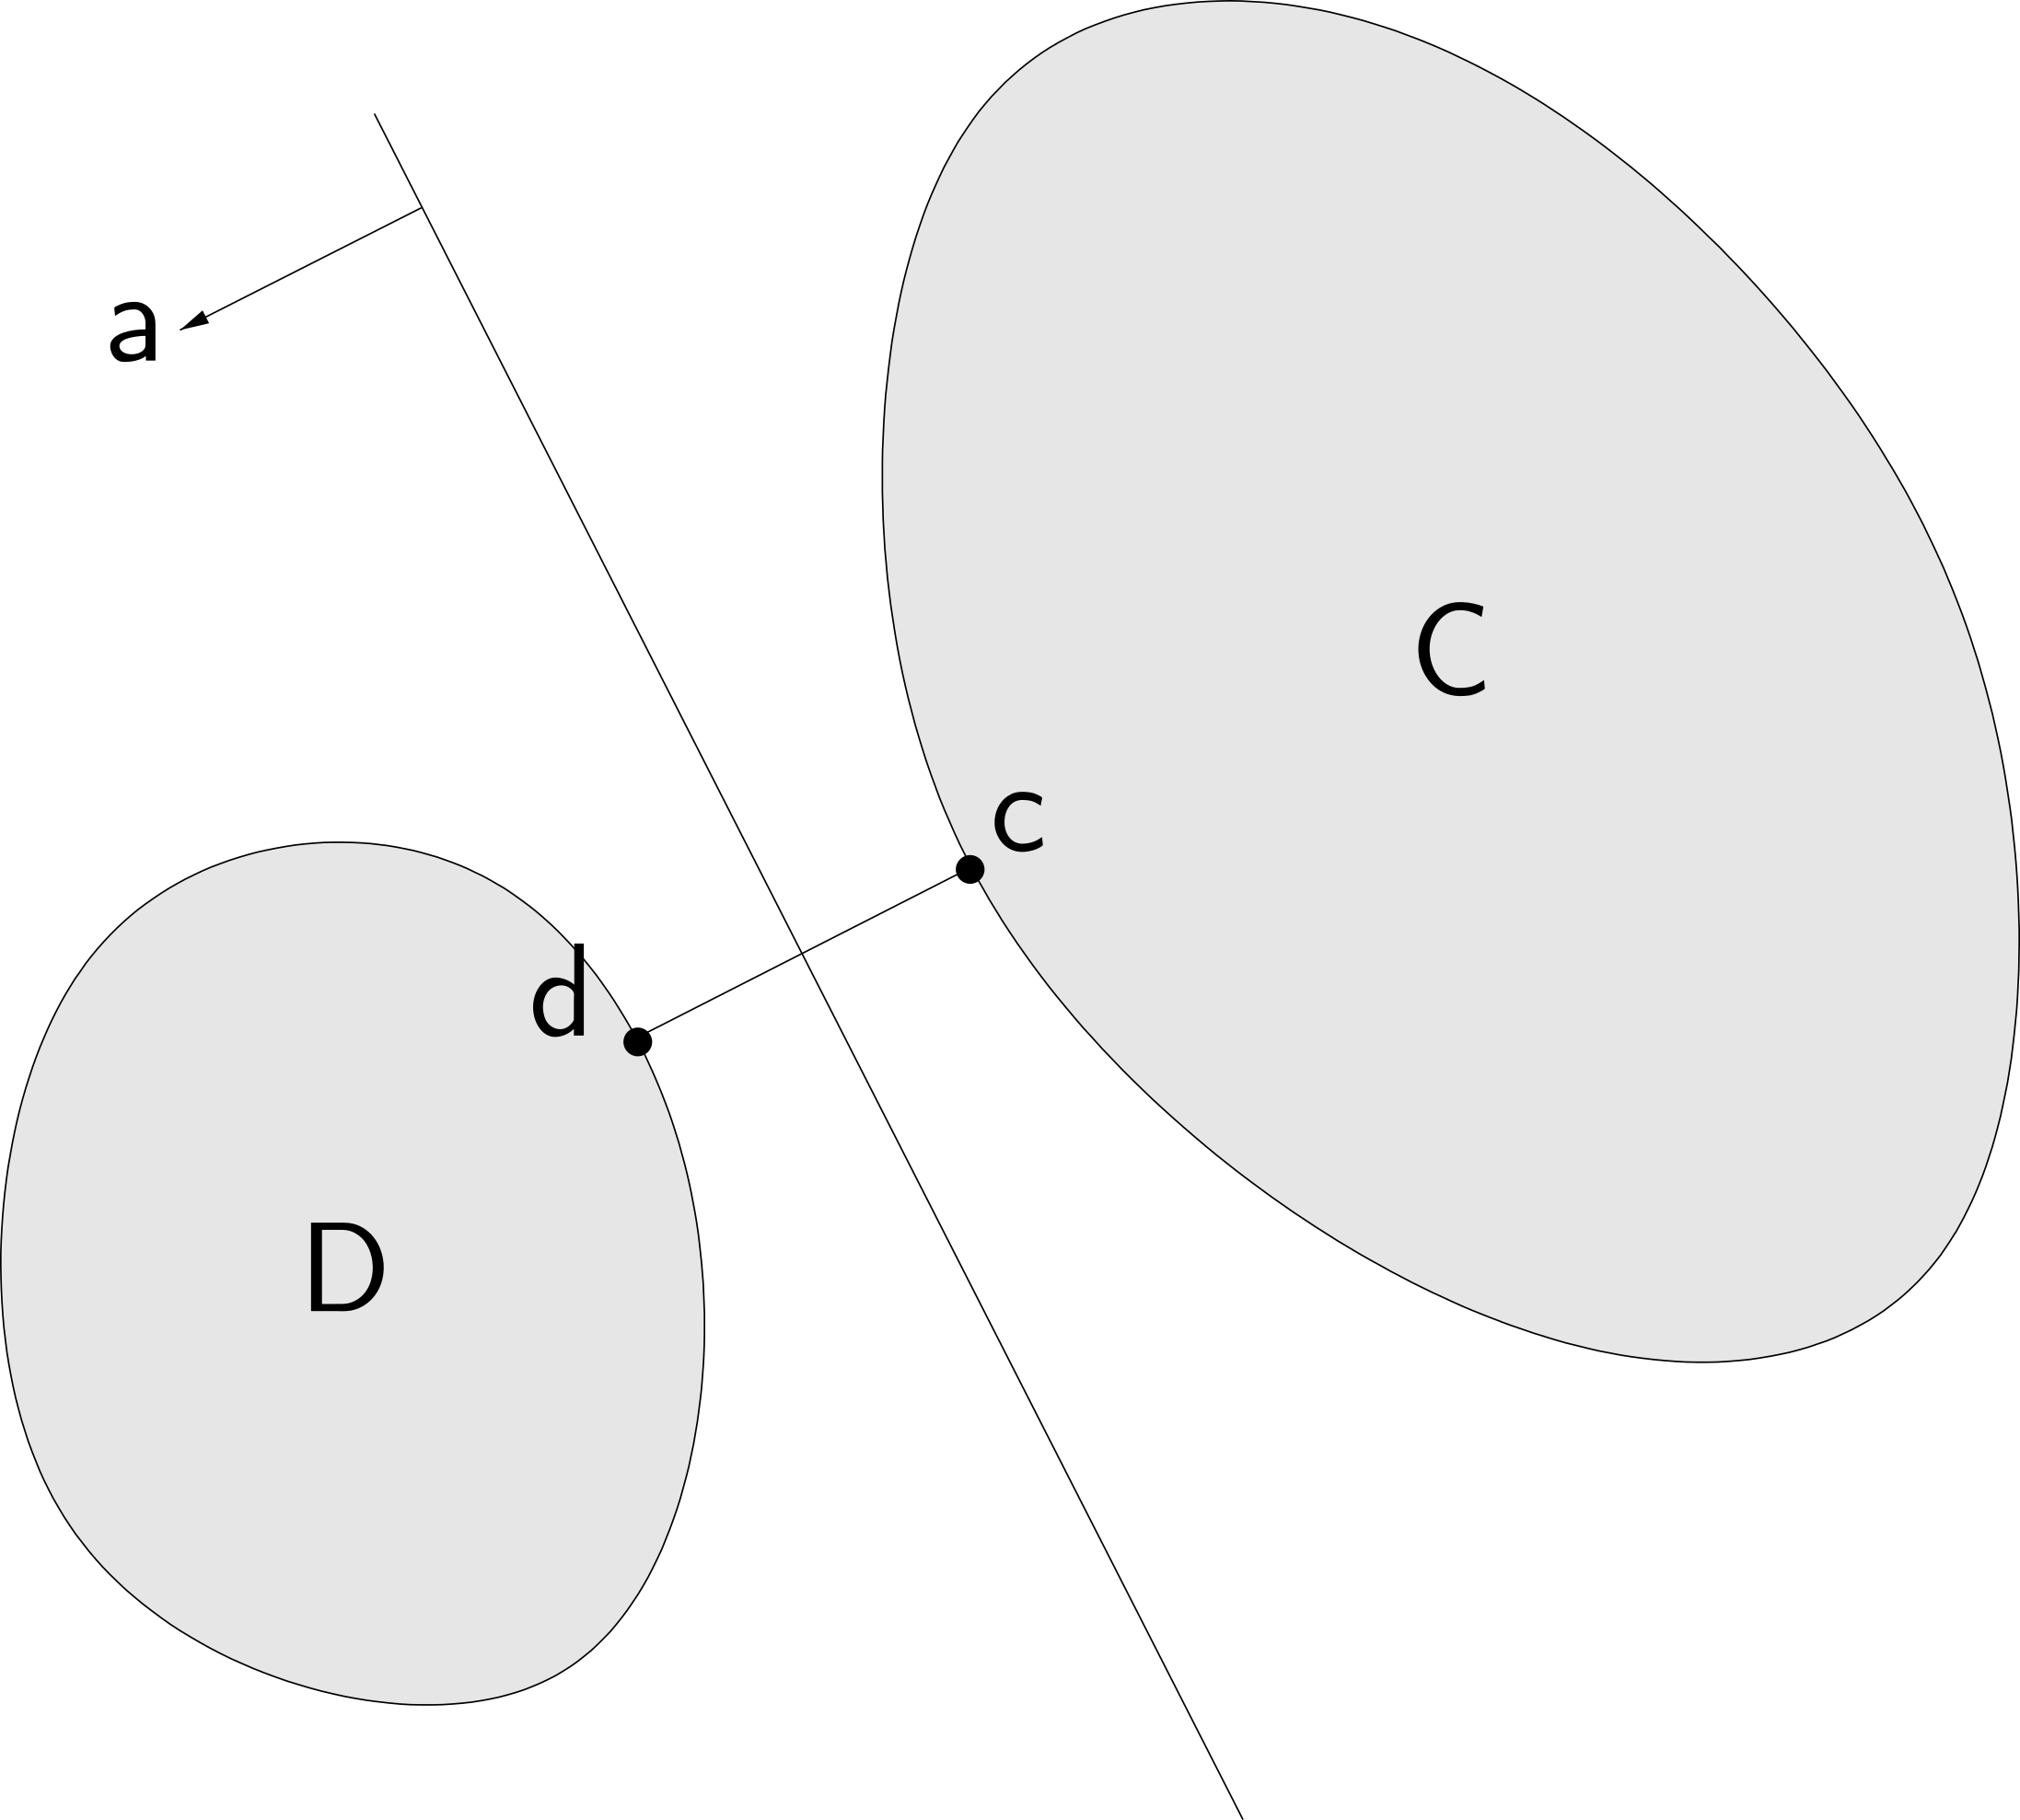
\includegraphics[width=.5\textwidth]{../Graphics/048.png}\hfil

\clearpage
\hfil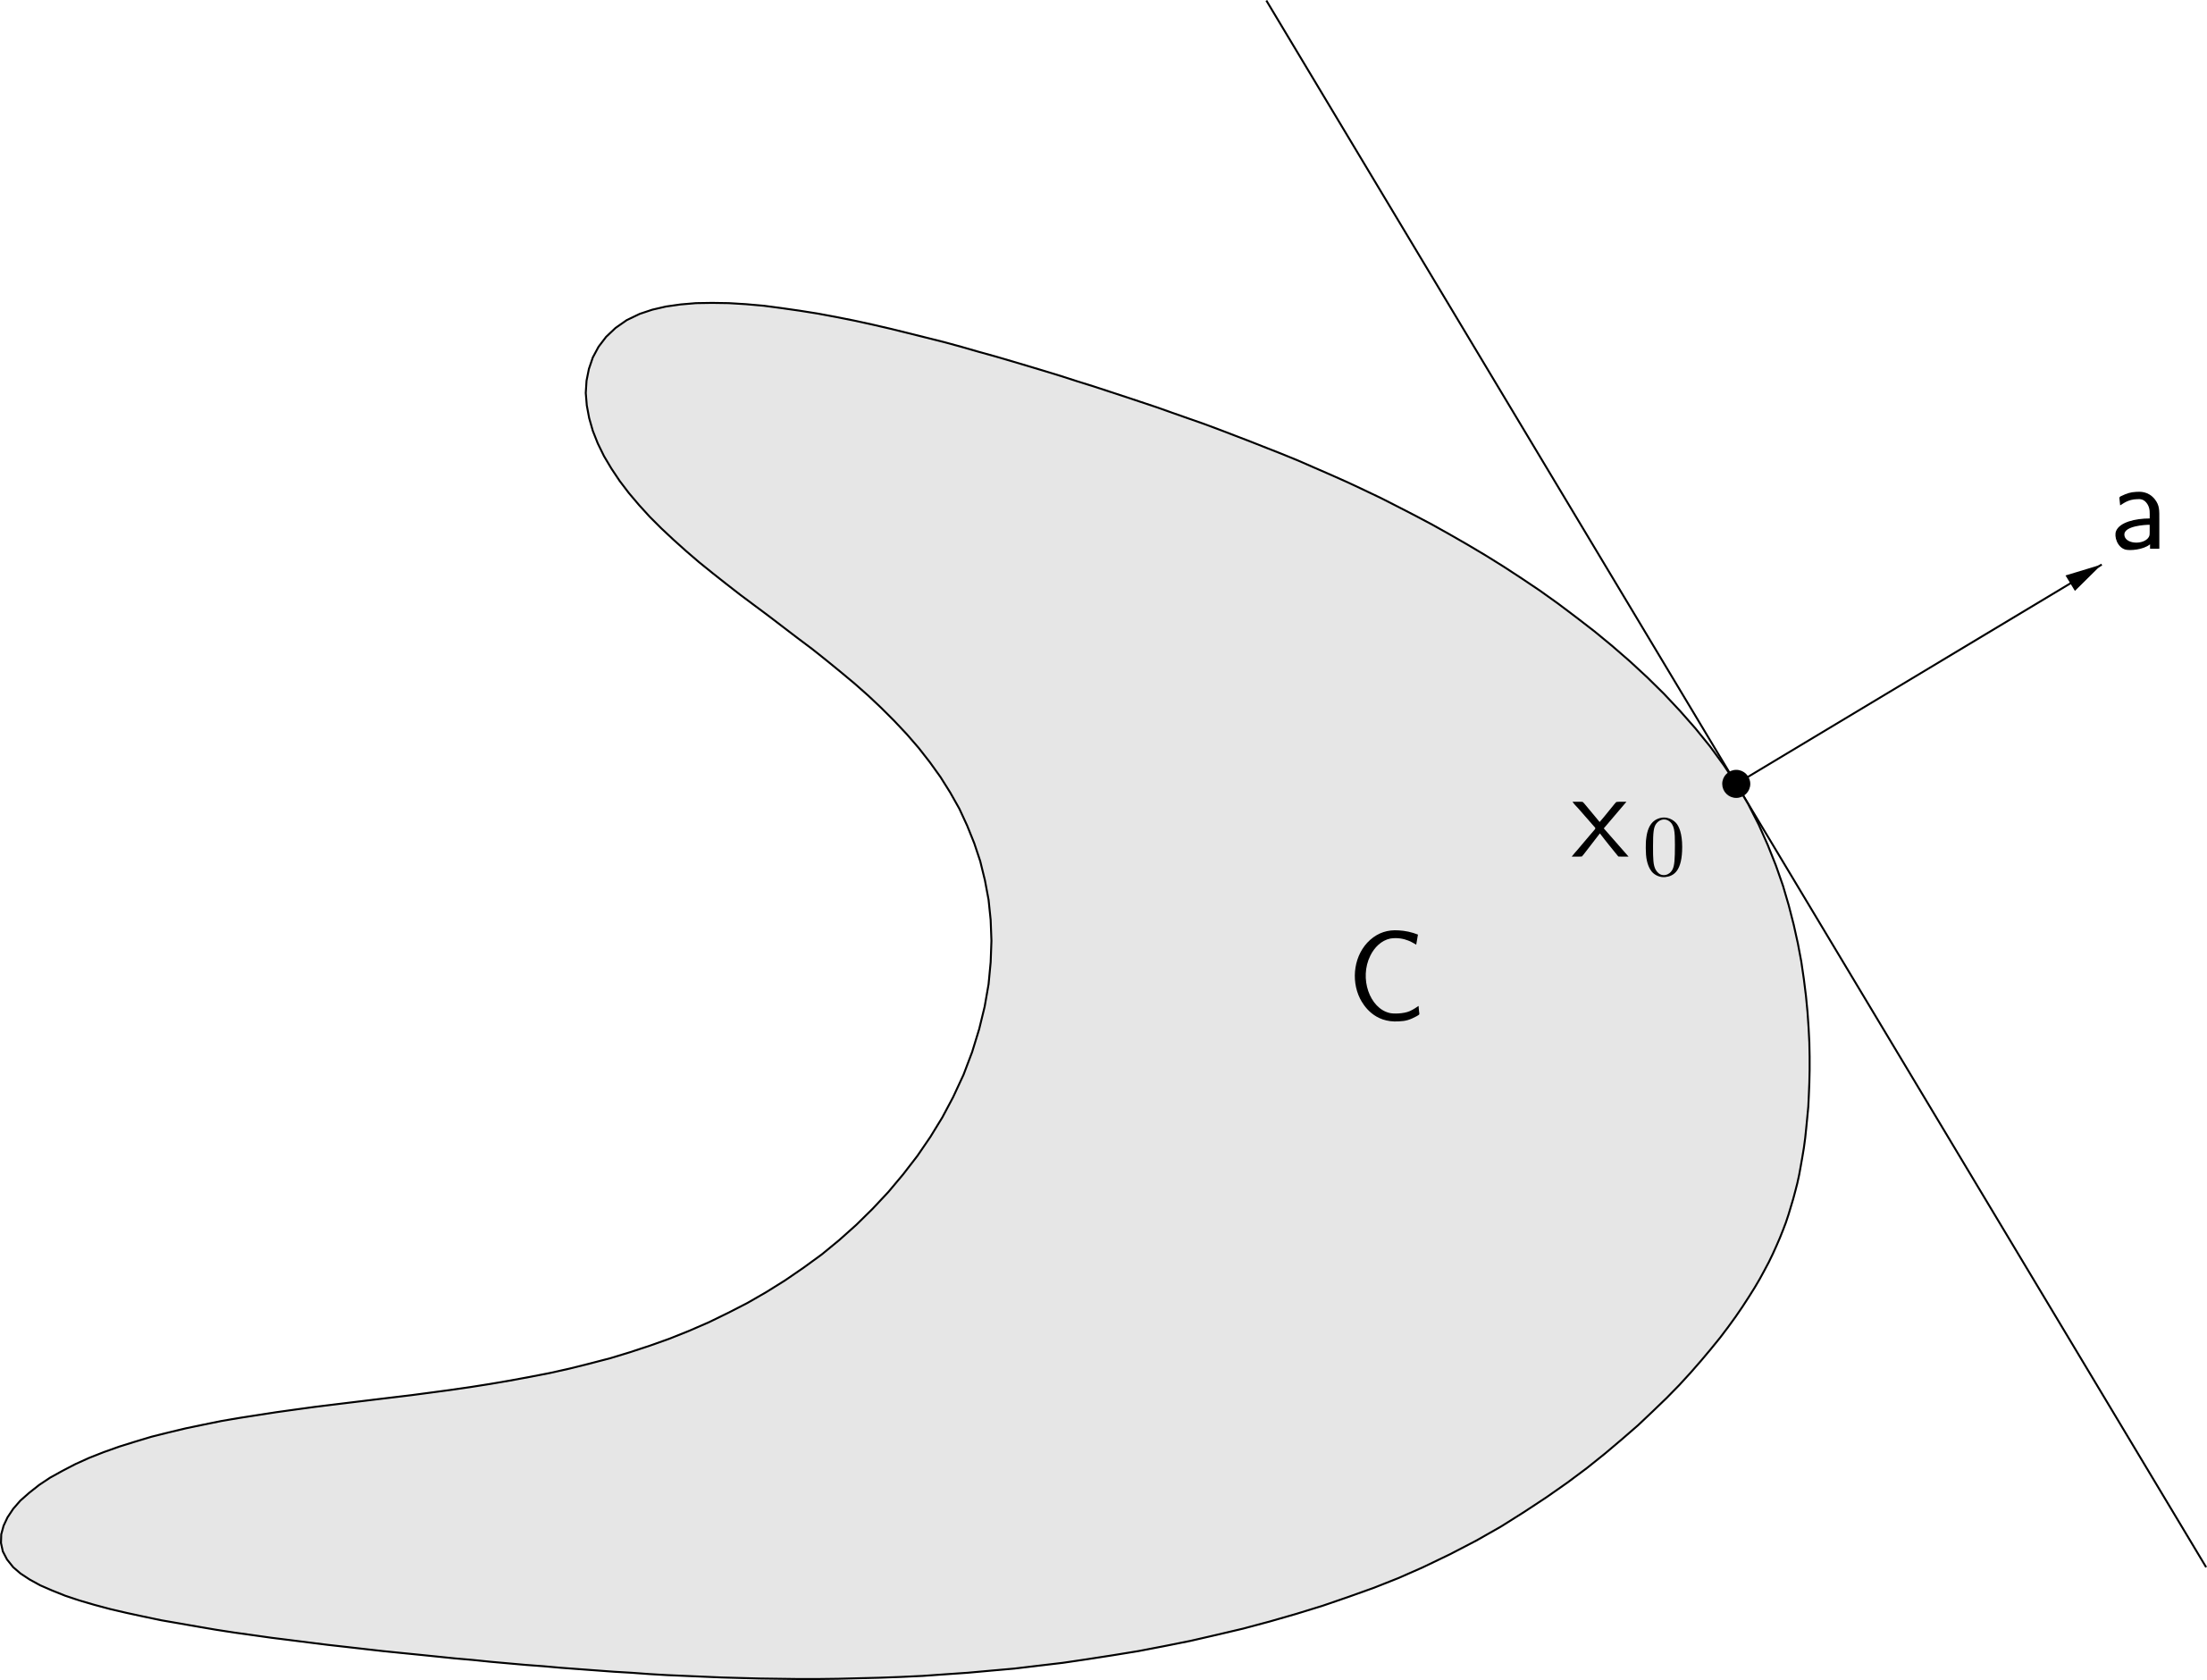
\includegraphics[width=.5\textwidth]{../Graphics/051.png}\hfil

\clearpage
\hfil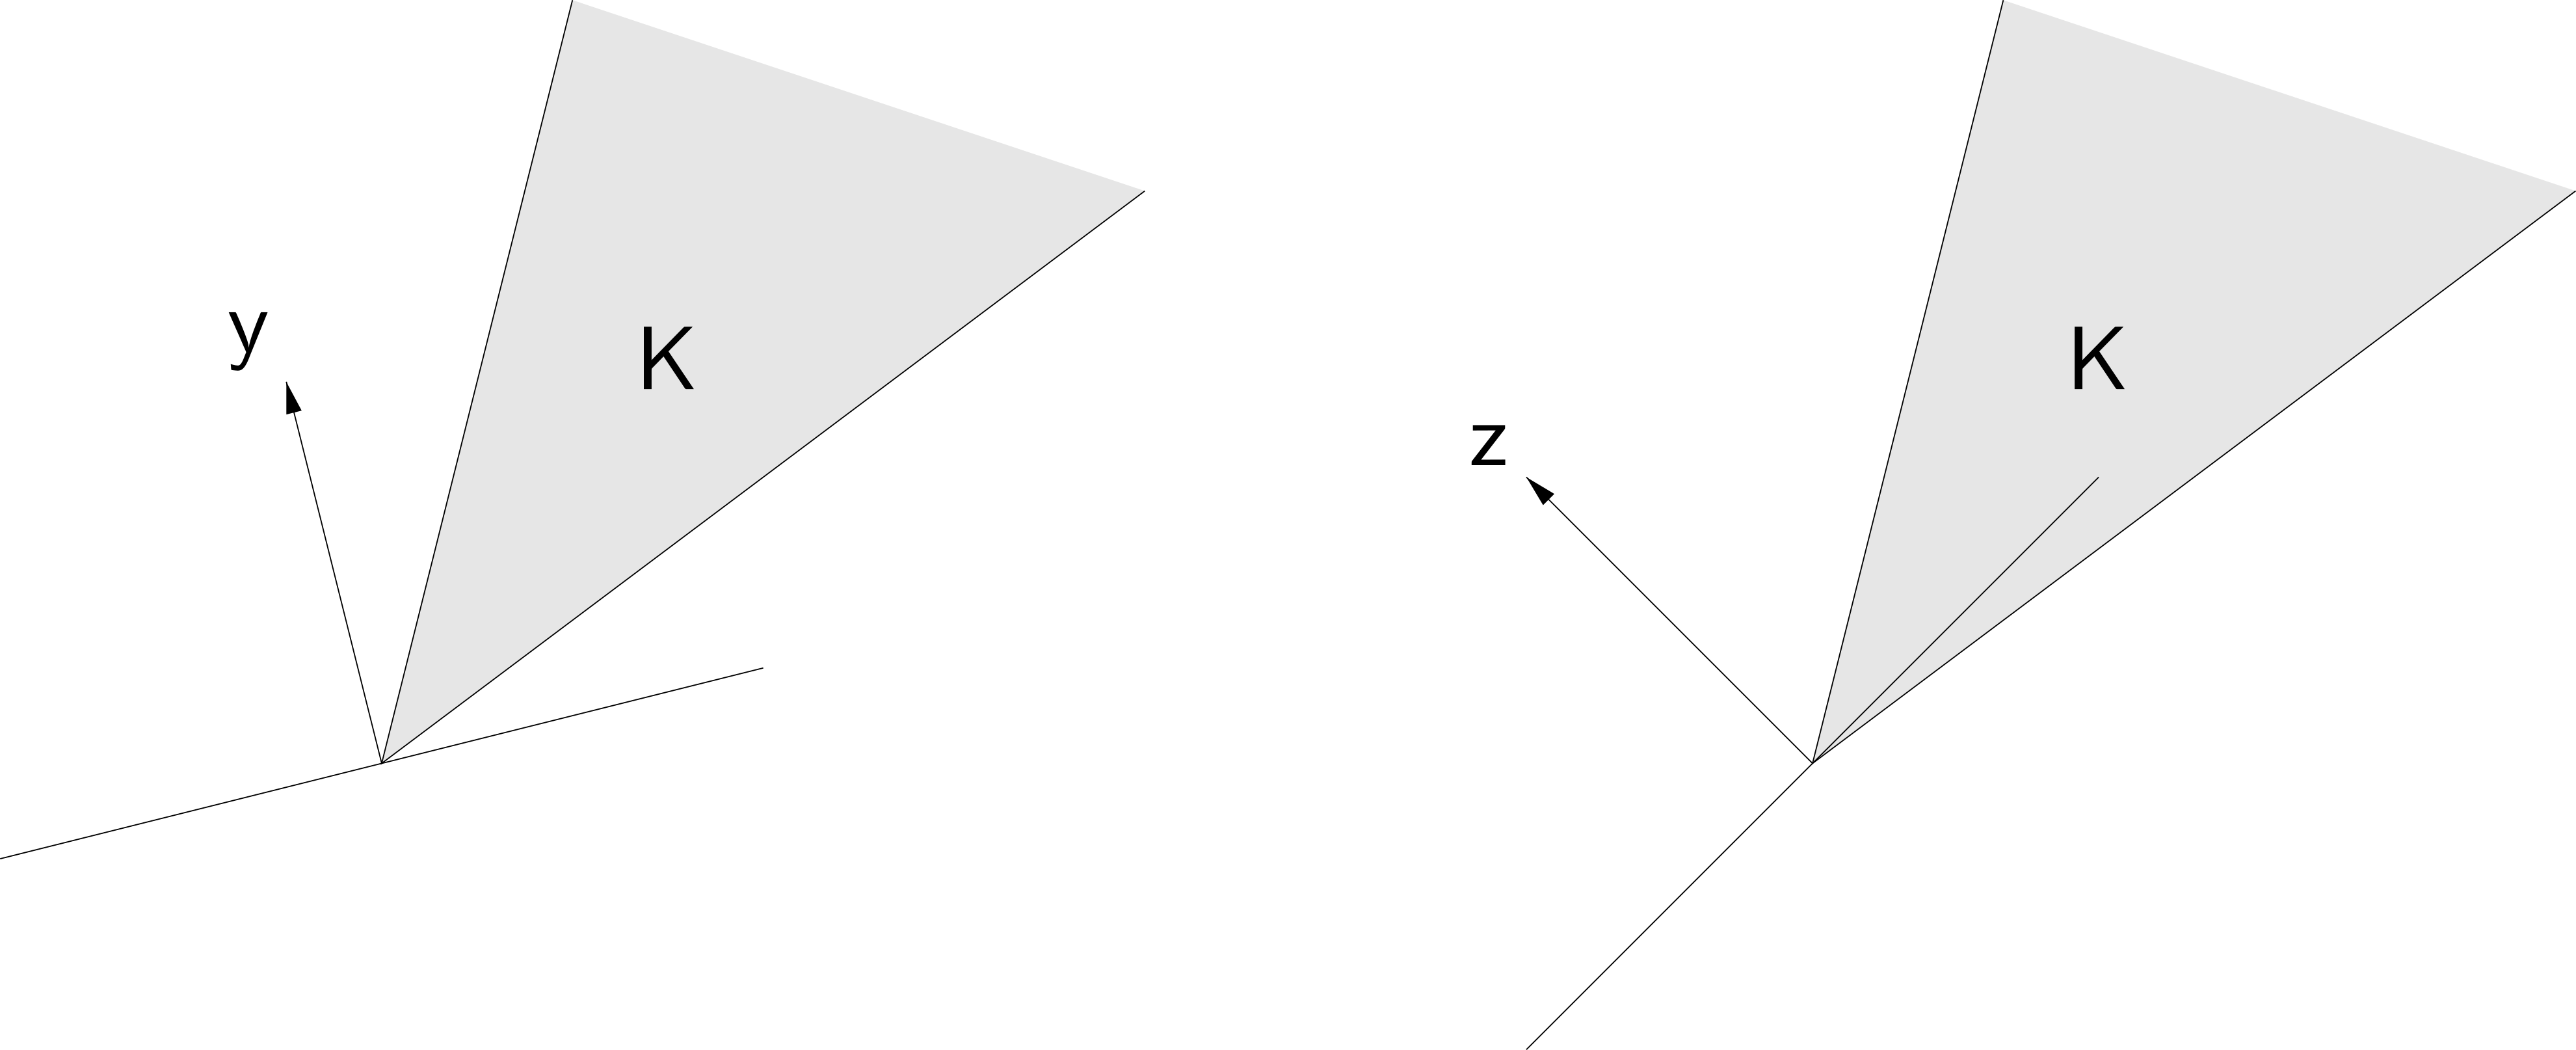
\includegraphics[width=.5\textwidth]{../Graphics/052.png}\hfil

\clearpage
\hfil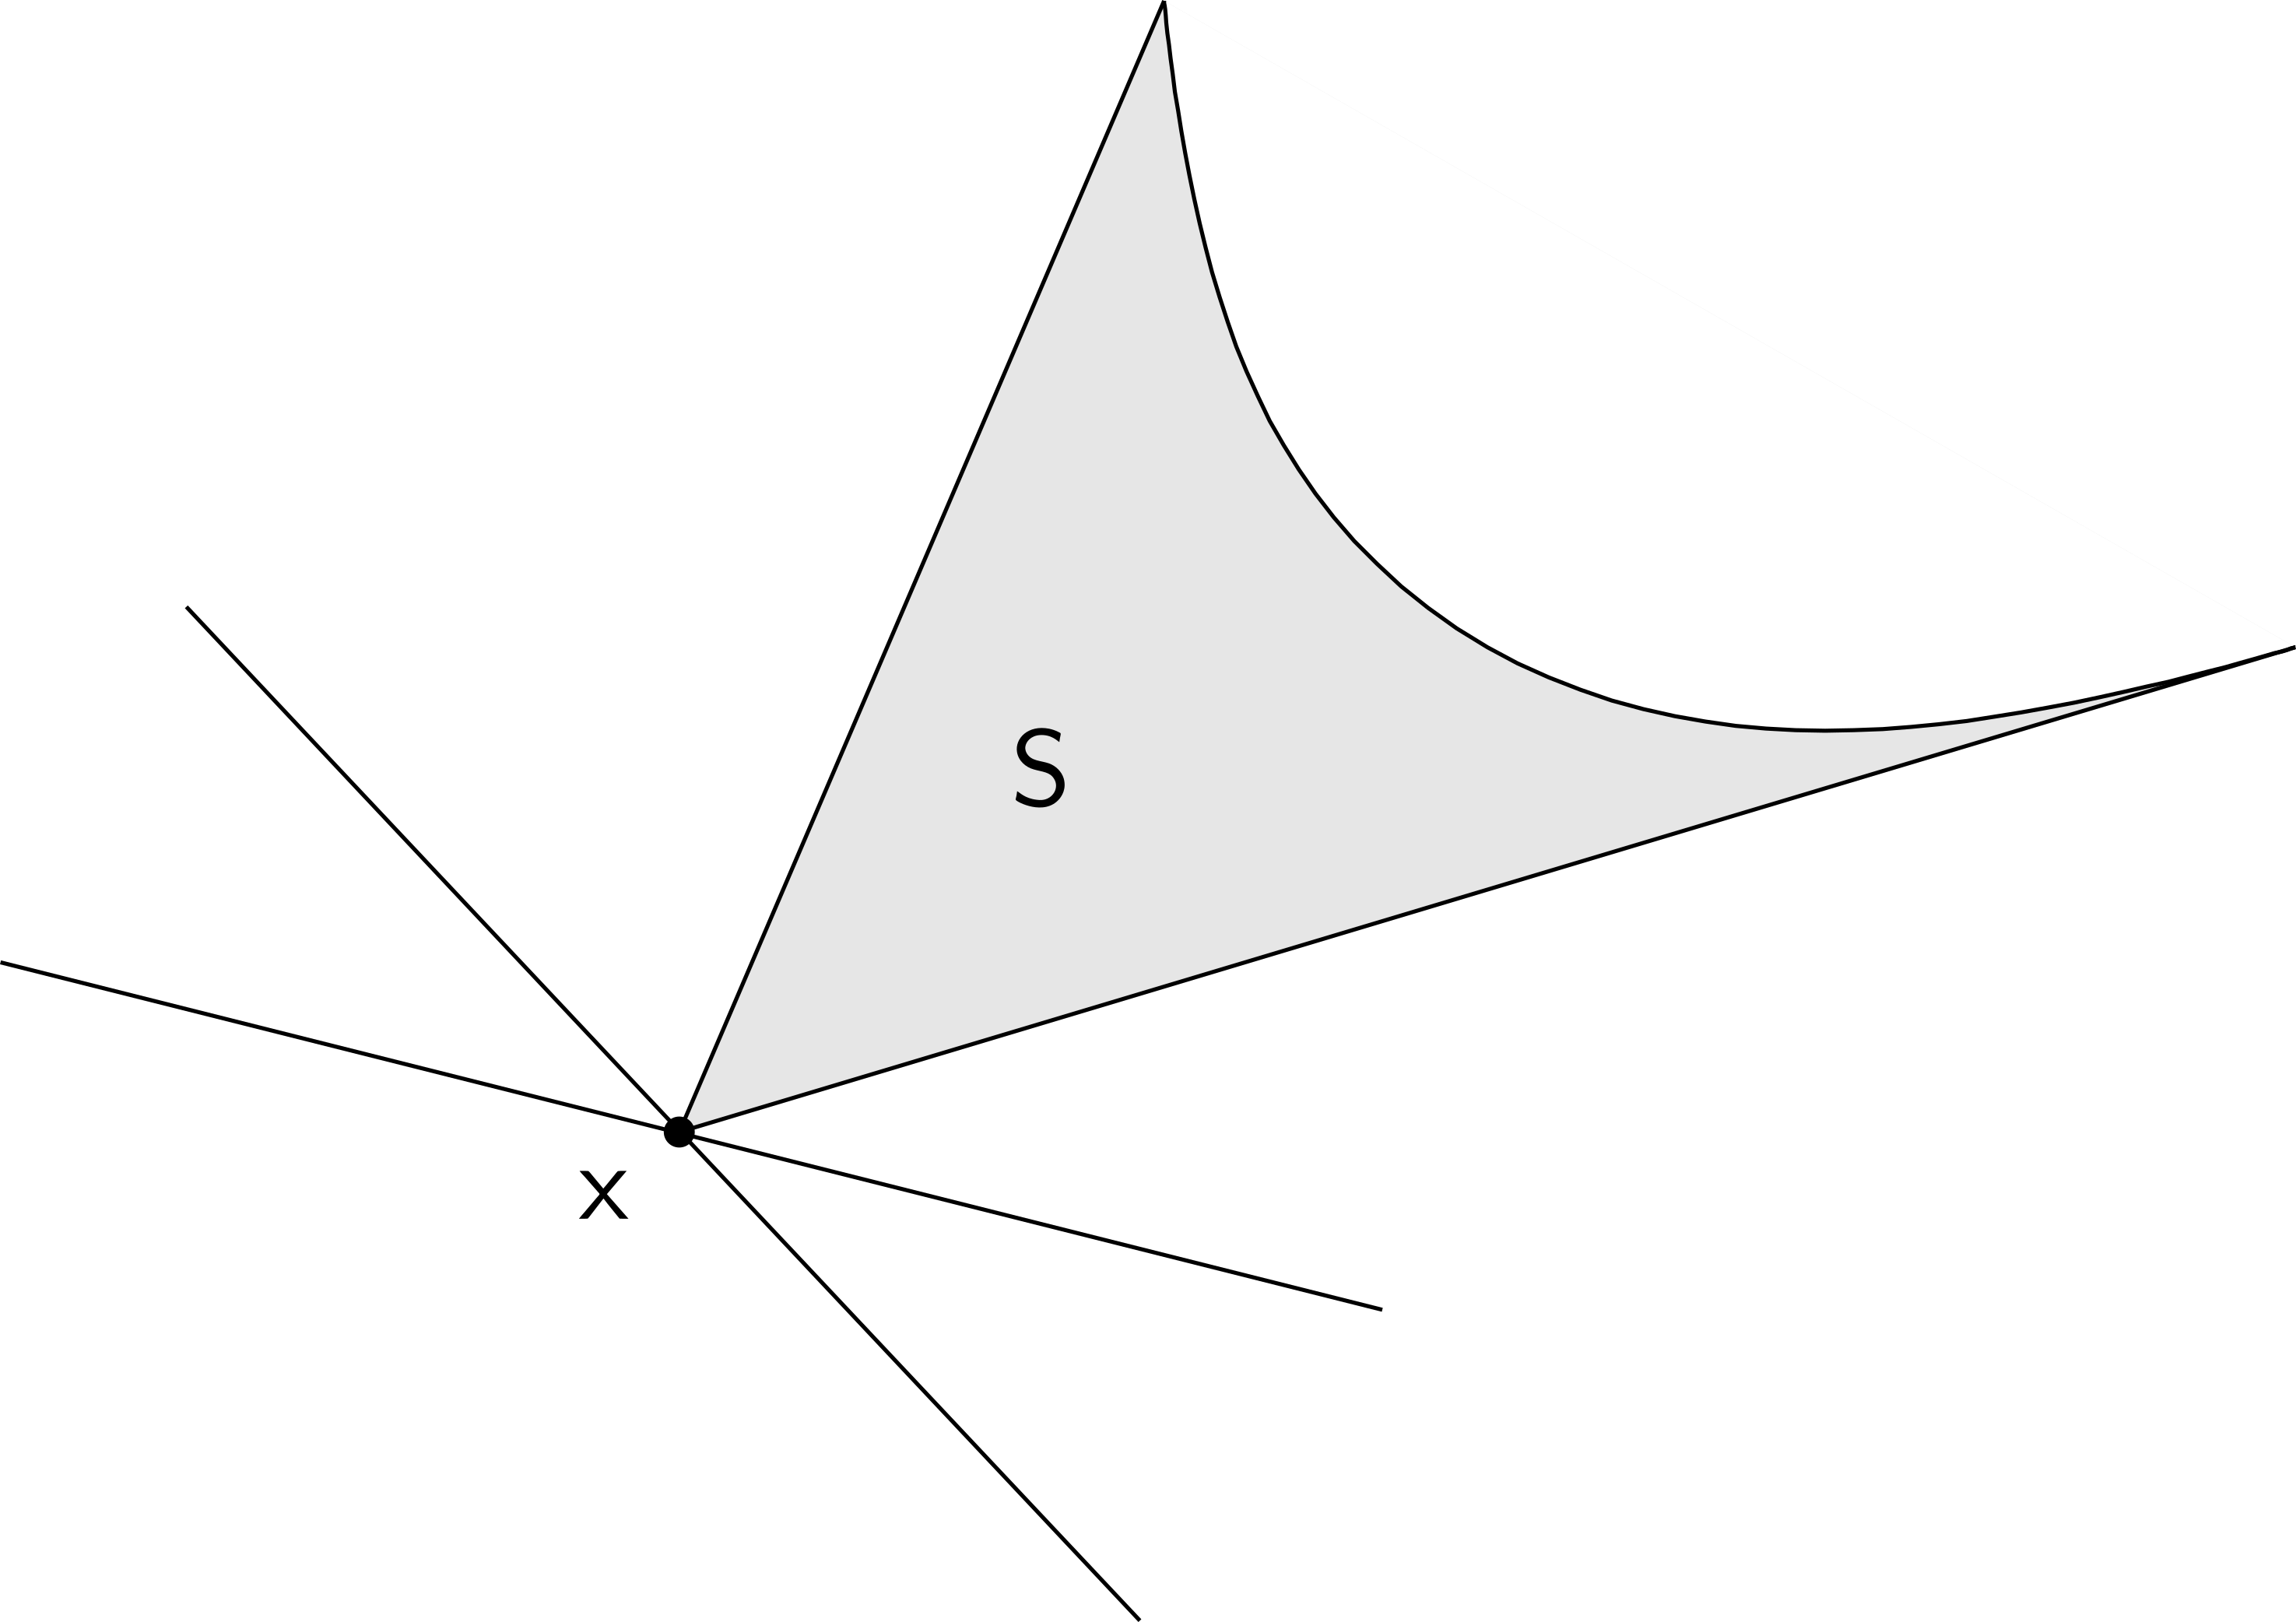
\includegraphics[width=.5\textwidth]{../Graphics/055.png}\hfil

\clearpage
\hfil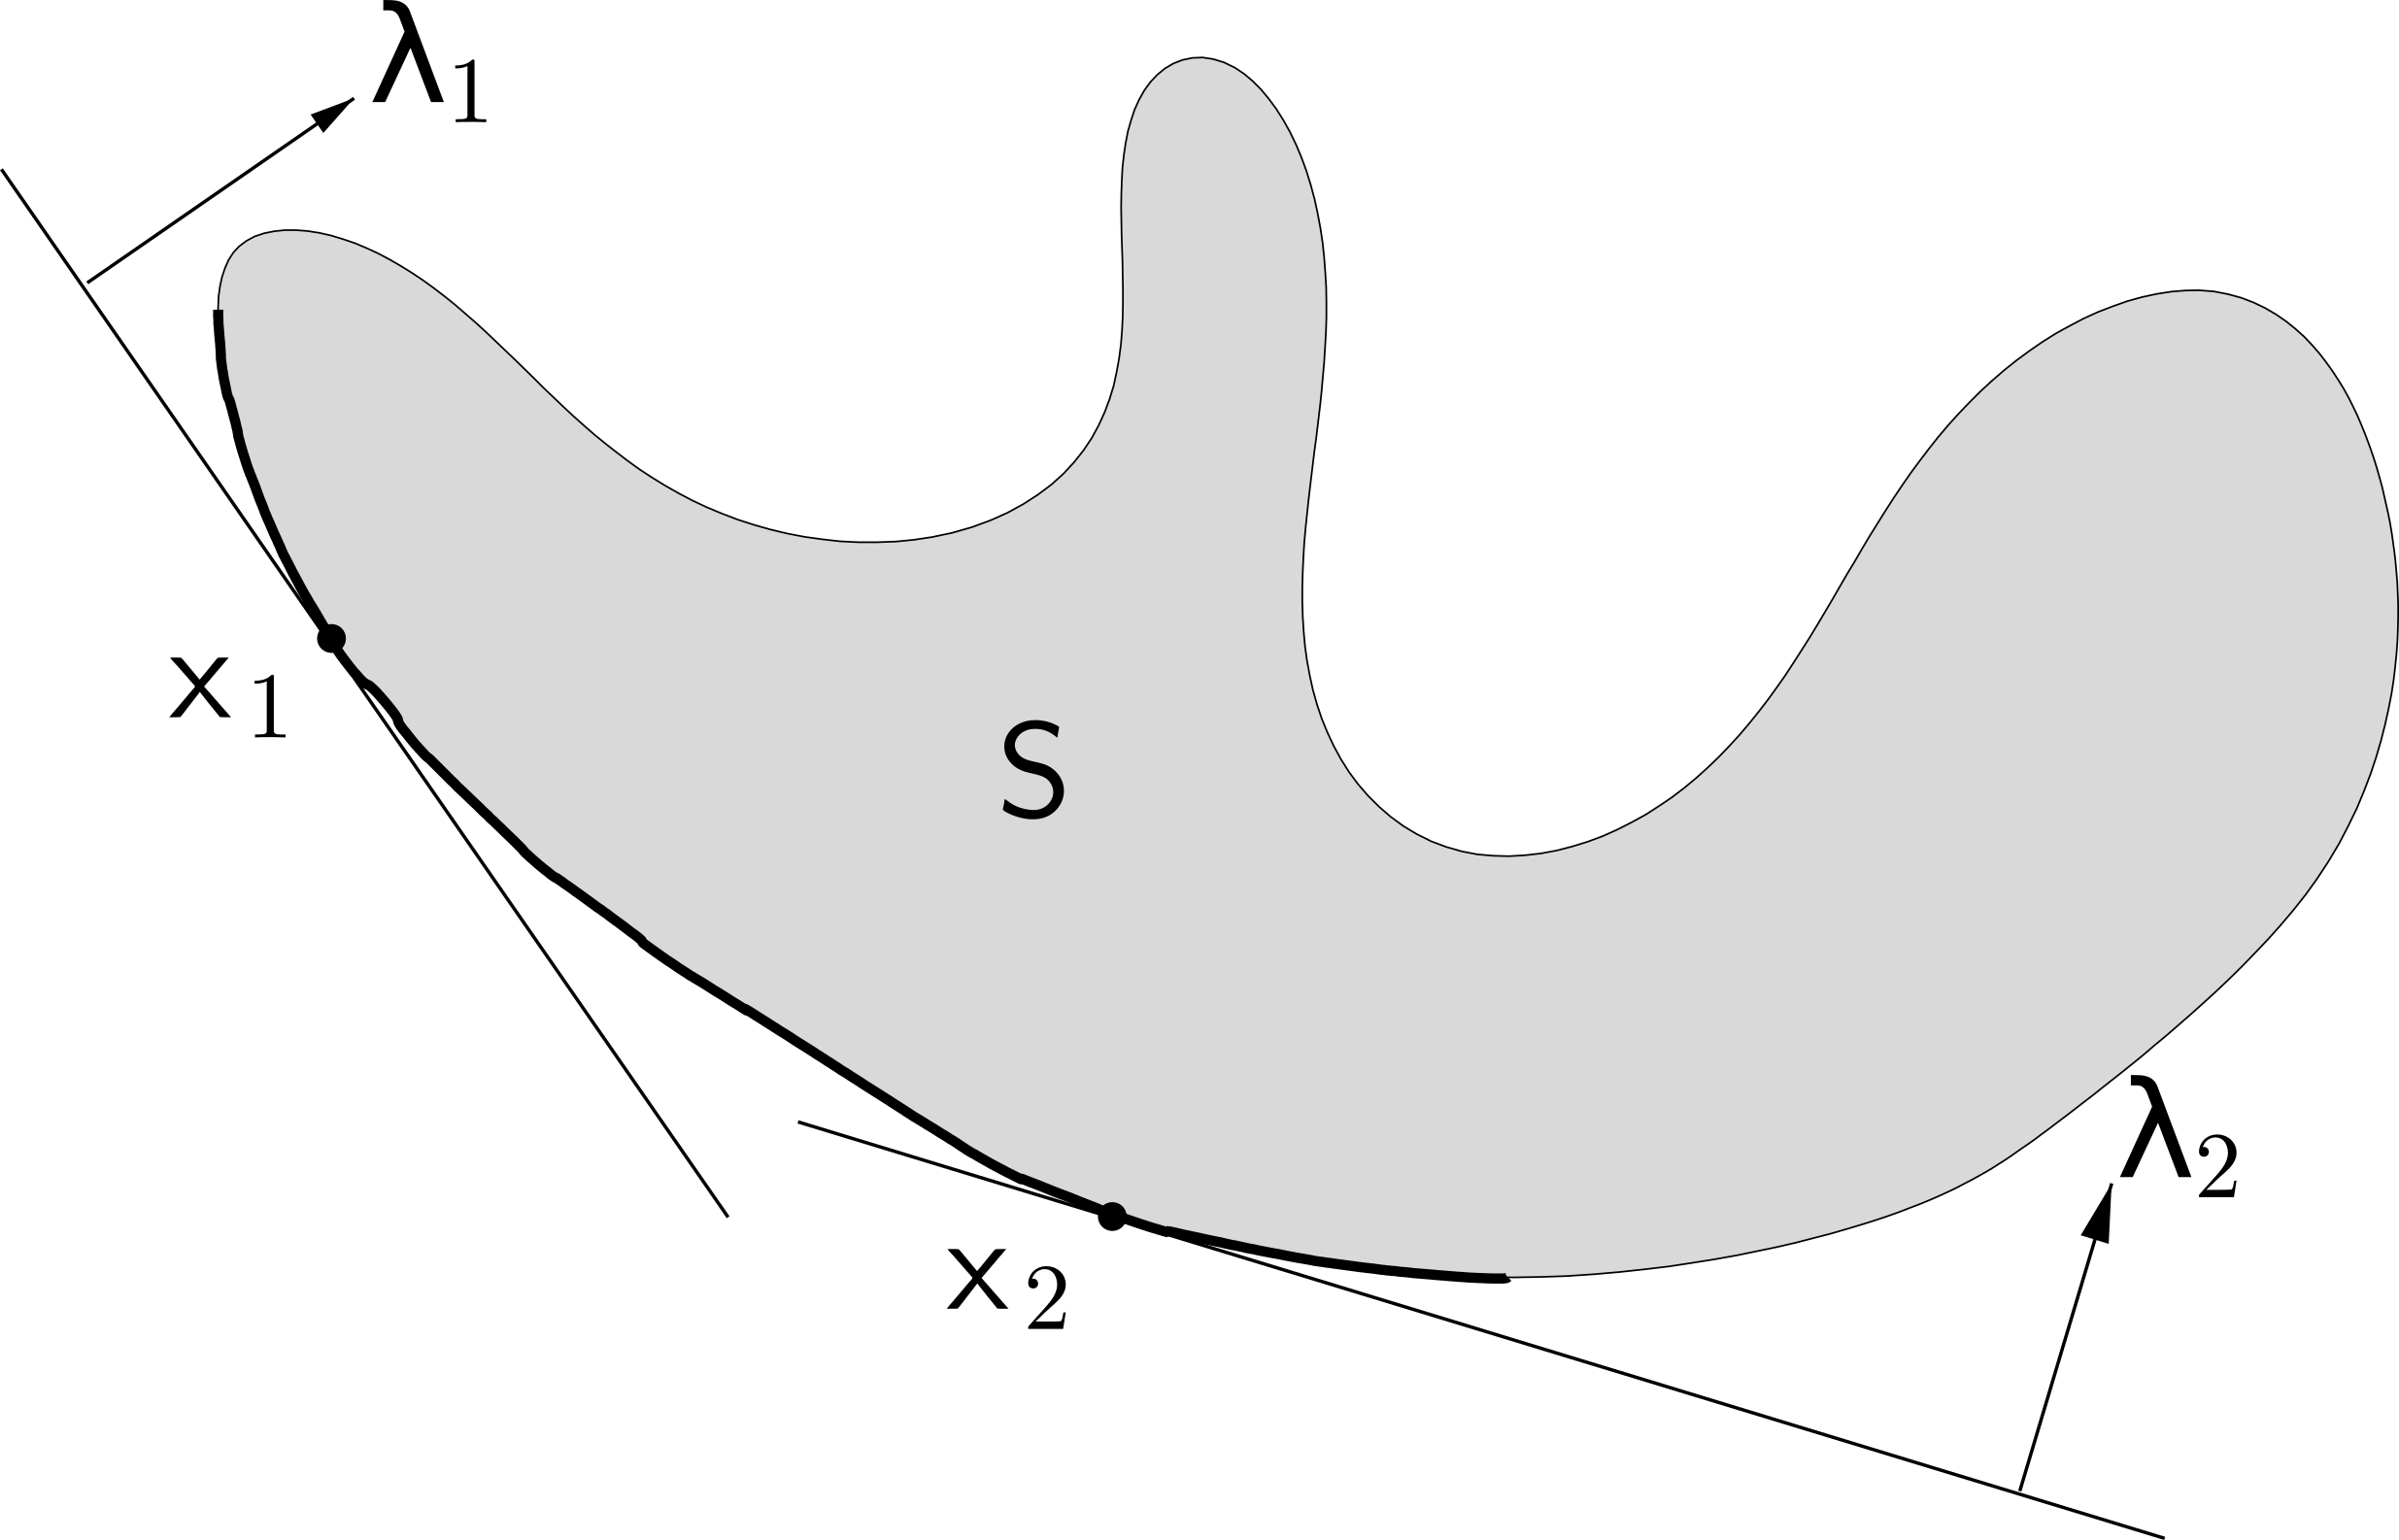
\includegraphics[width=.5\textwidth]{../Graphics/056a.png}\hfil

\clearpage
\hfil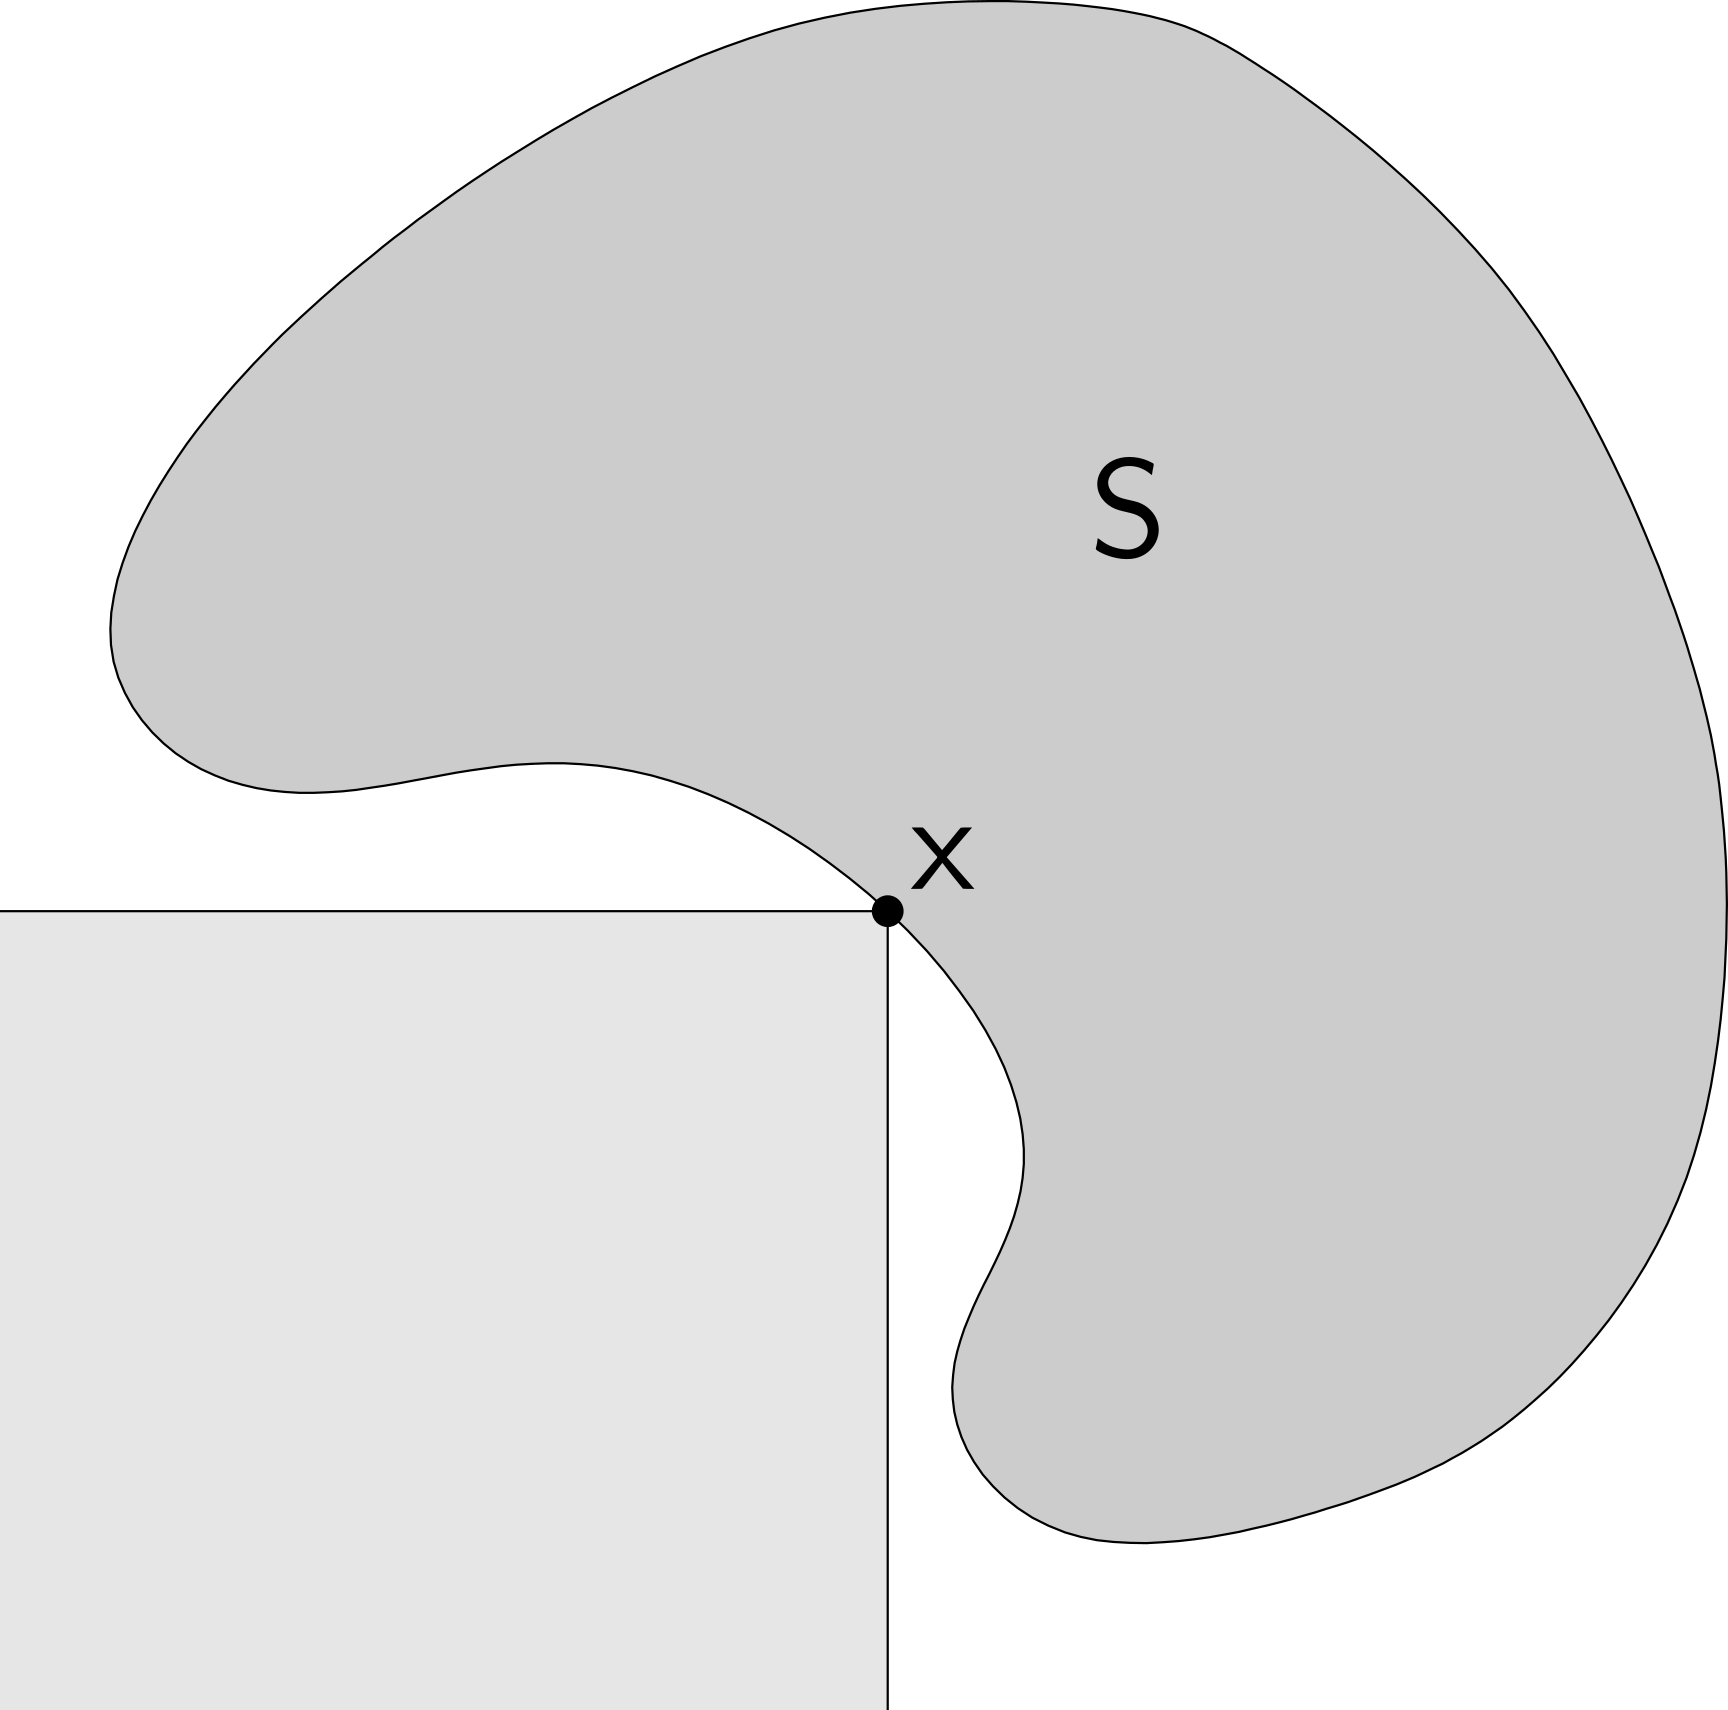
\includegraphics[width=.5\textwidth]{../Graphics/056b.png}\hfil

\clearpage
\hfil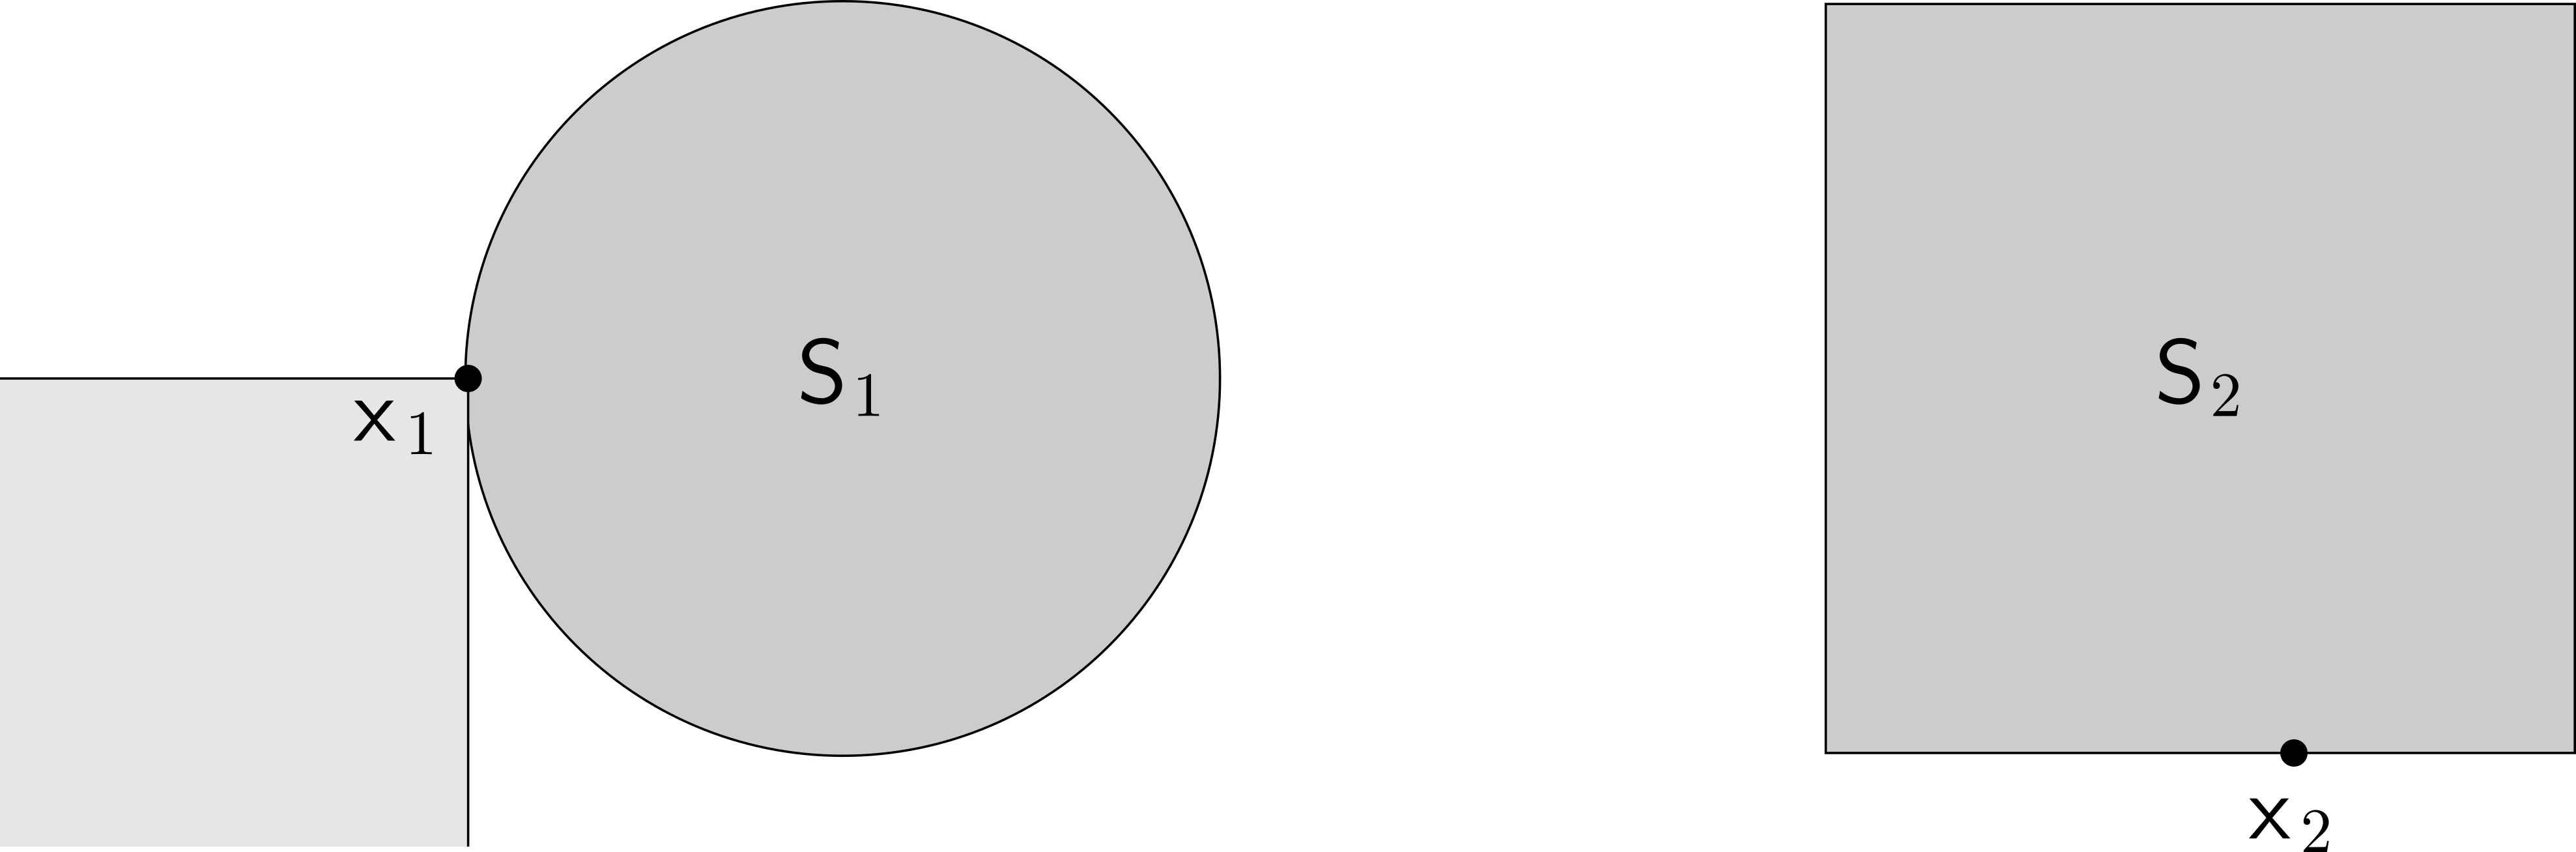
\includegraphics[width=.5\textwidth]{../Graphics/057.png}\hfil

\clearpage
\hfil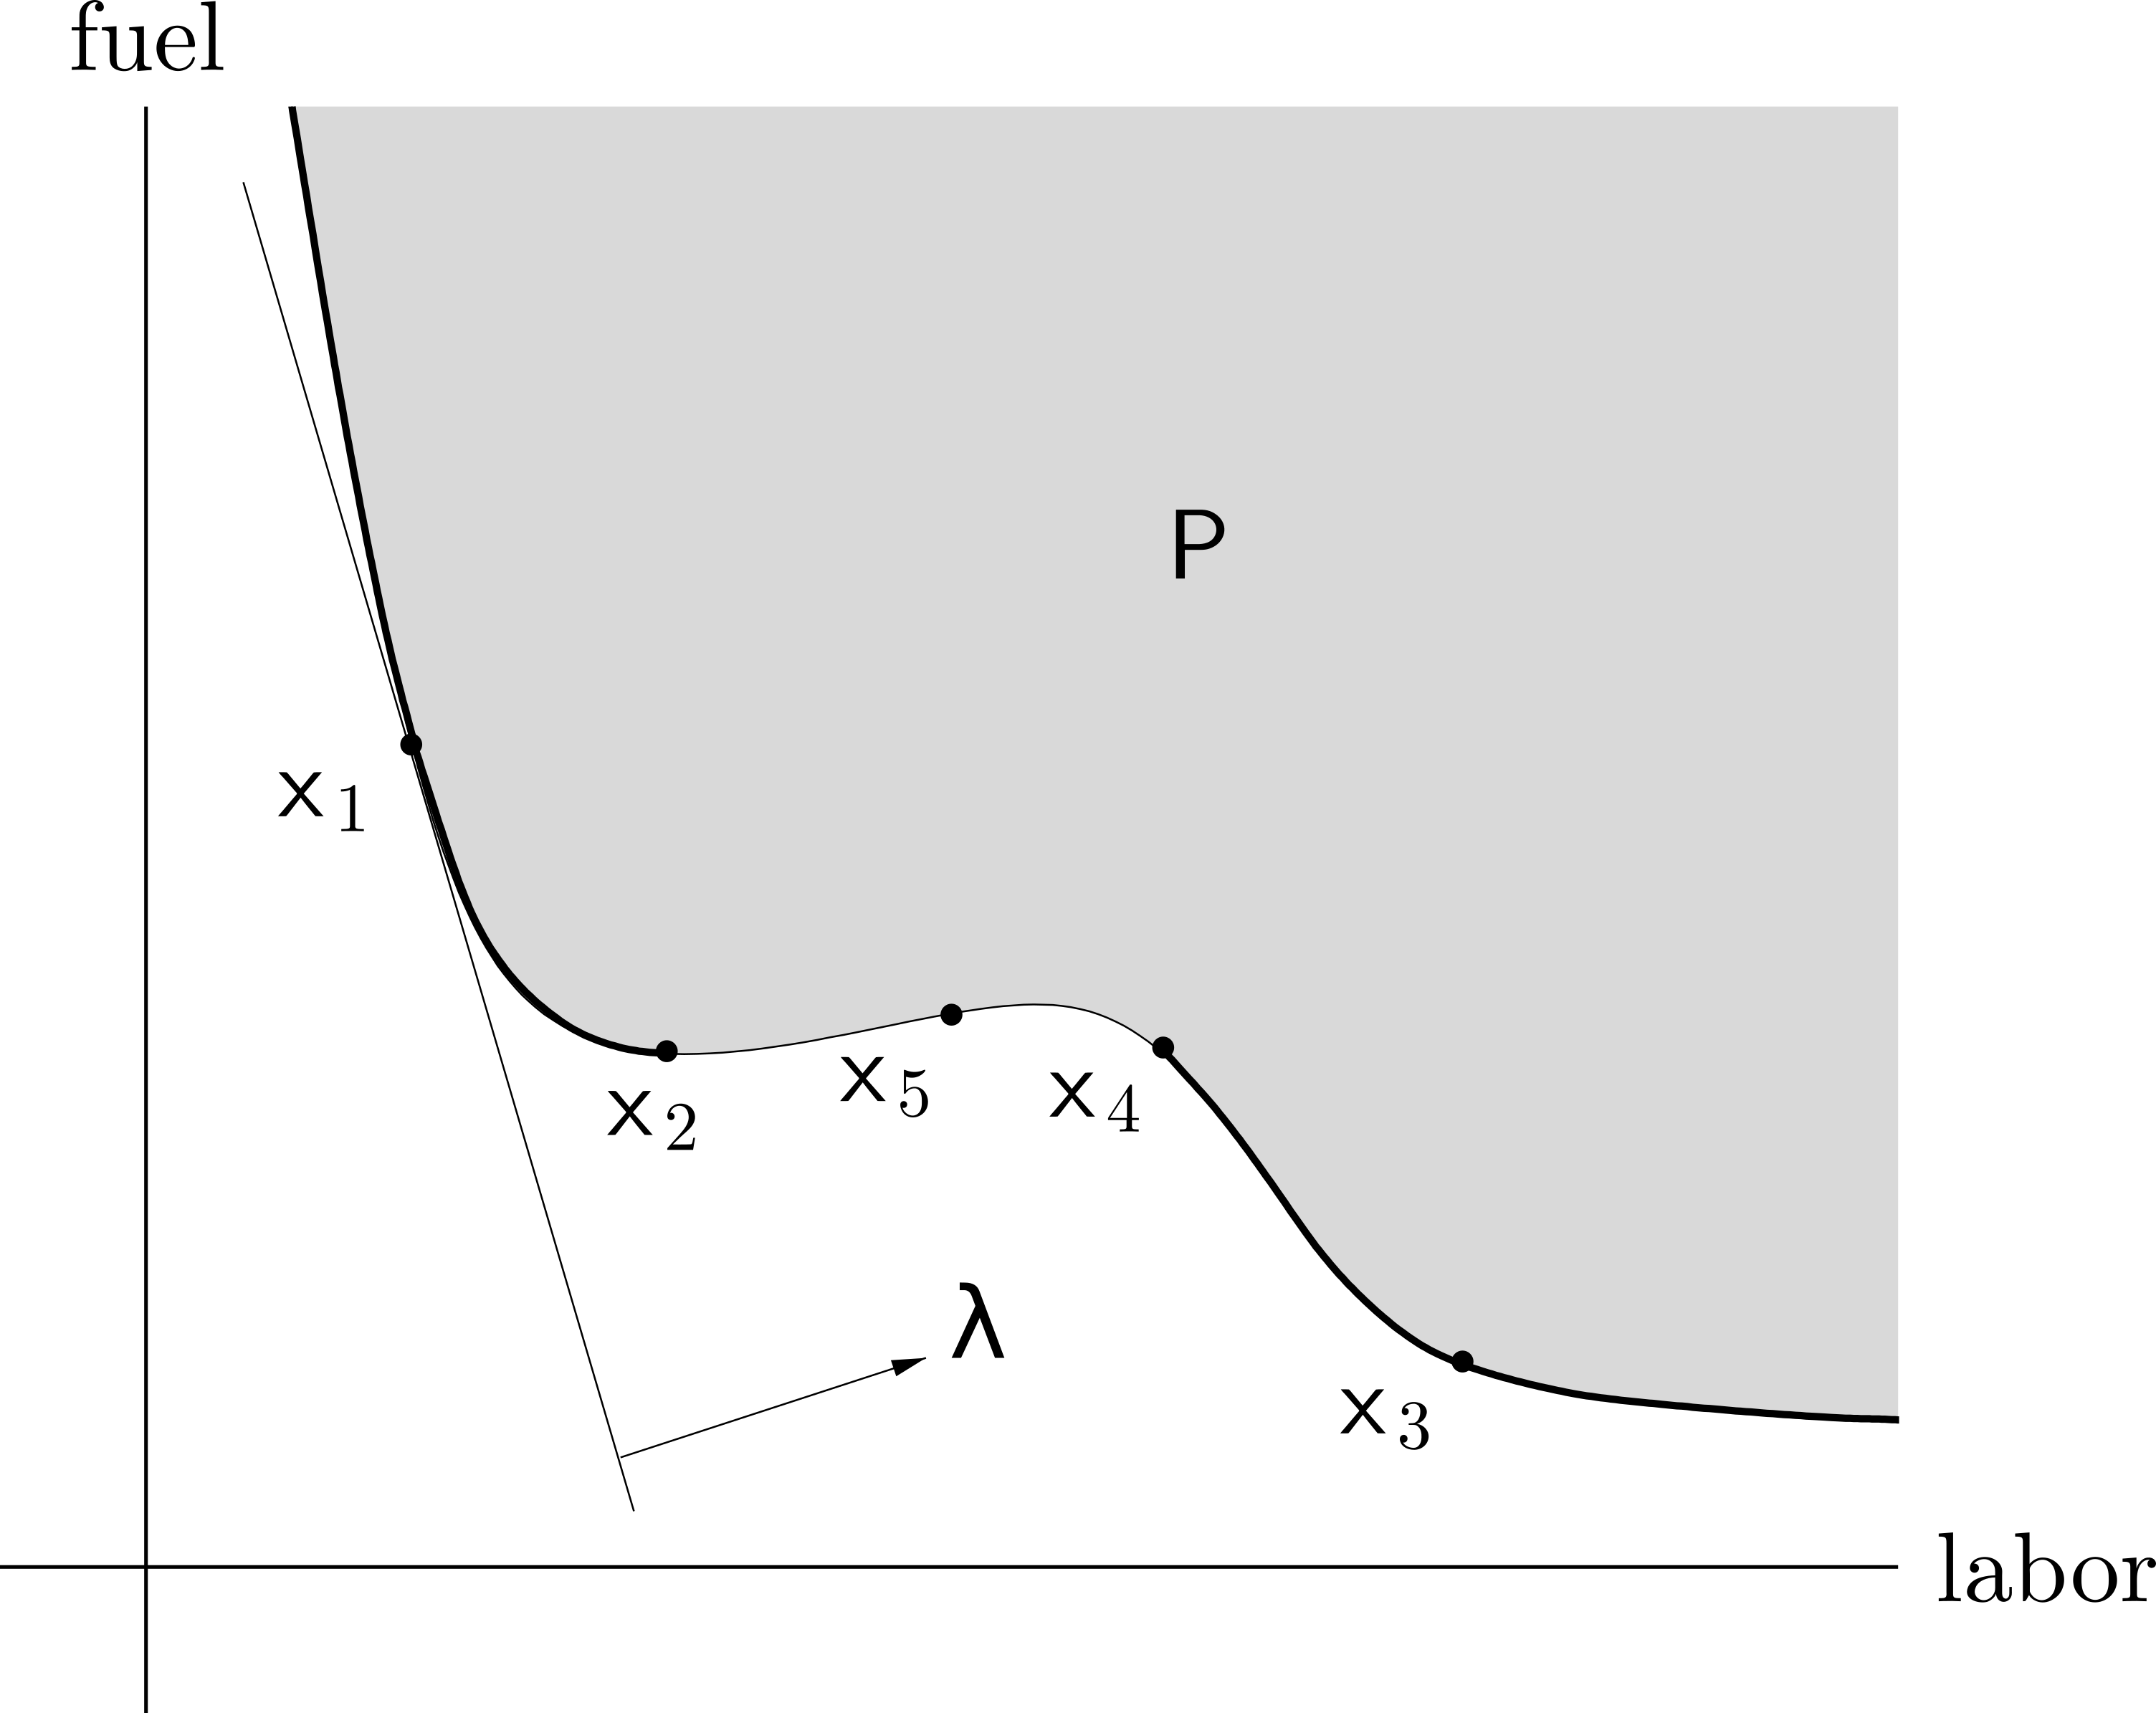
\includegraphics[width=.5\textwidth]{../Graphics/058.png}\hfil

%%% Local Variables:
%%% mode: latex
%%% TeX-master: "../LectureNotes-Optimization"
%%% End:



\chapter{Convex functions}

\clearpage
\section{Basic properties and examples}

\clearpage
\section{Operations that preserve convexity}

\clearpage
\section{The conjugate function}

\clearpage
\section{Quasiconvex functions}

\clearpage
\section{Log-concave and log-convex functions}

\clearpage
\section{Convexity with respect to generalized inequalities}


\clearpage
\hfil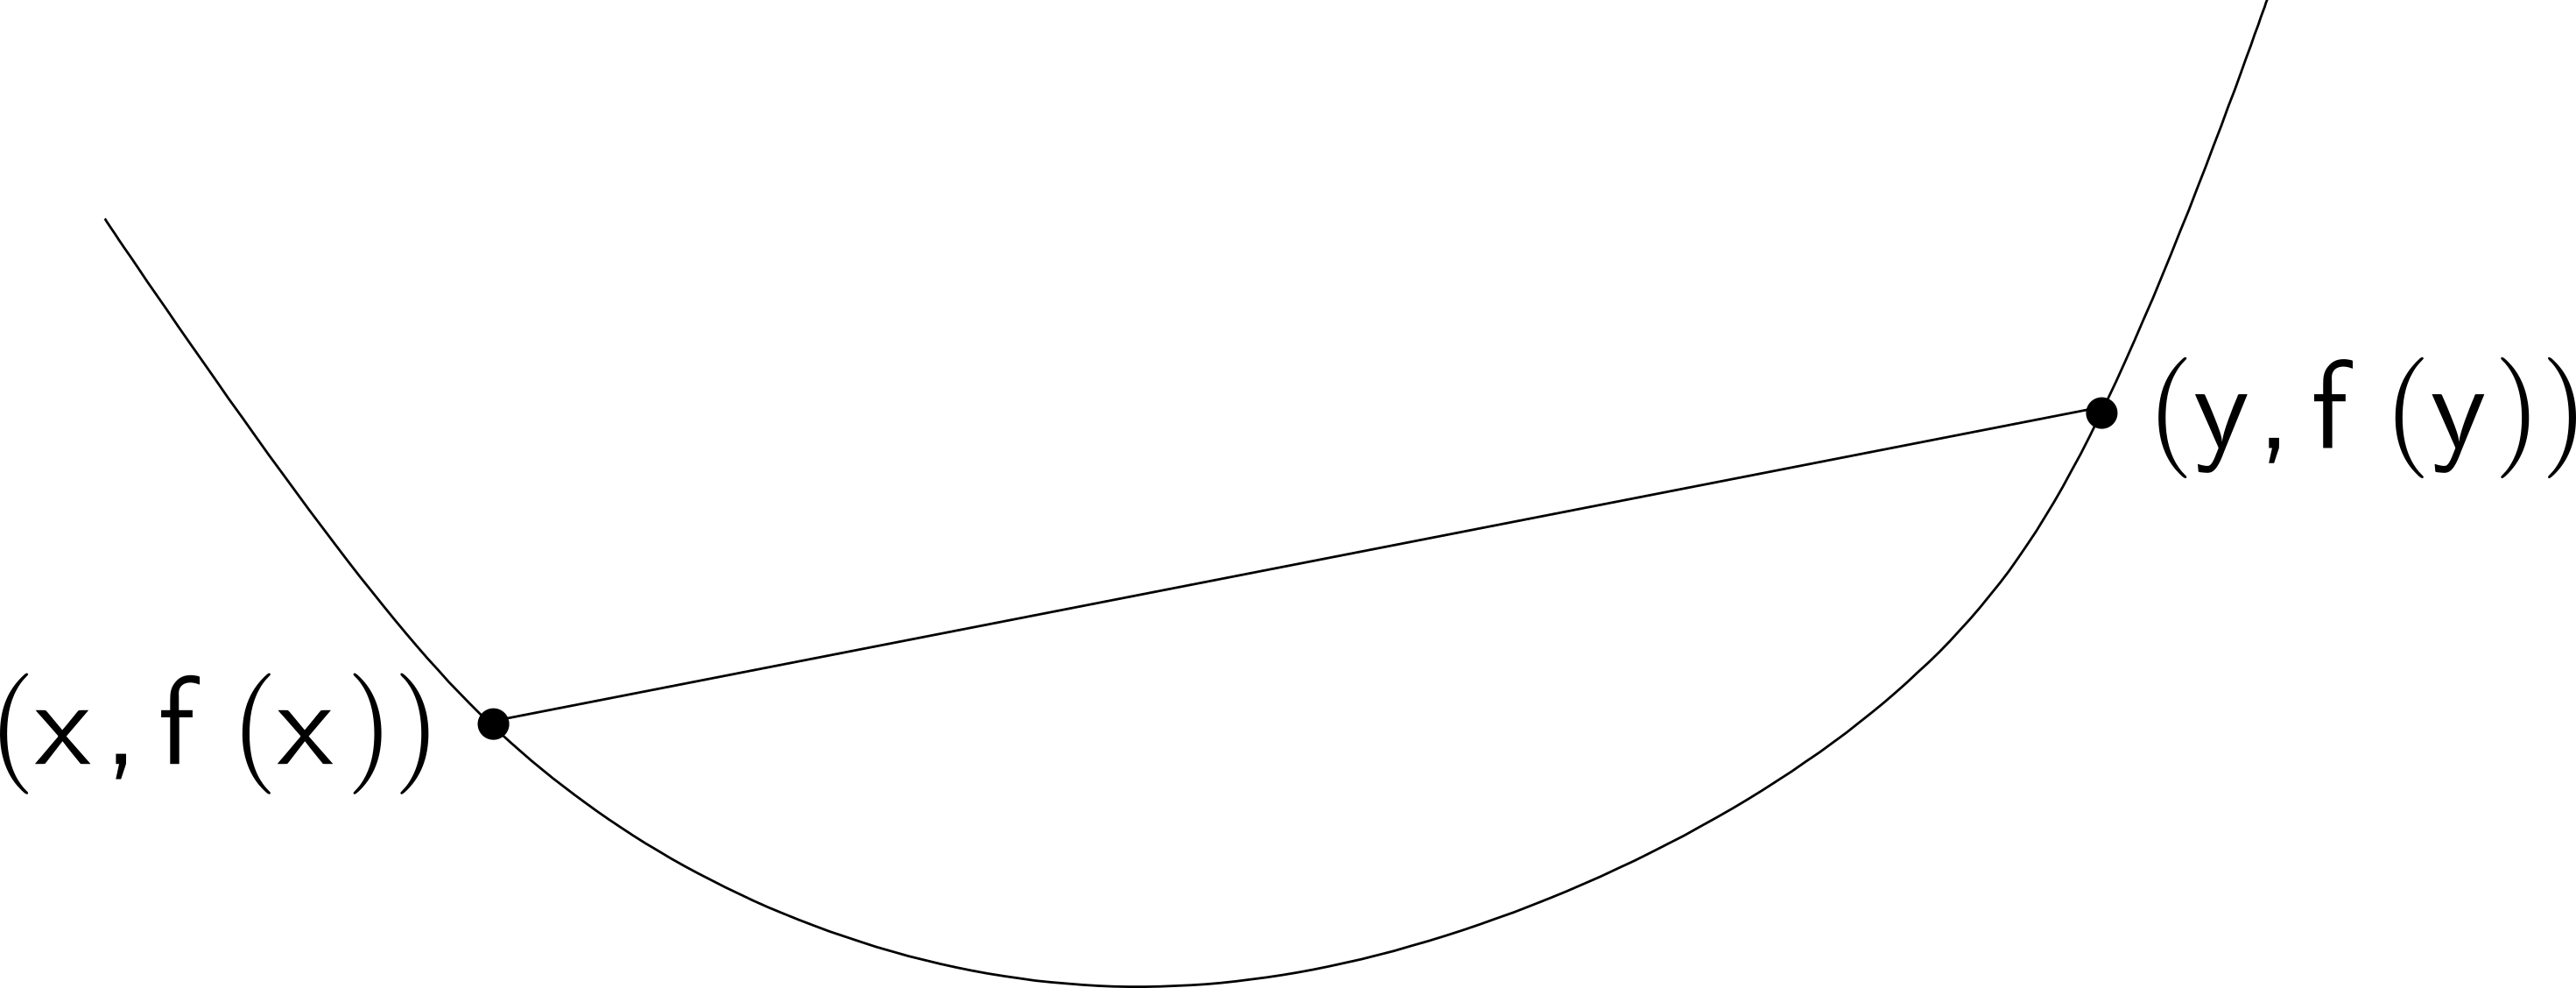
\includegraphics[width=.5\textwidth]{../Graphics/067.png}\hfil

\clearpage
\hfil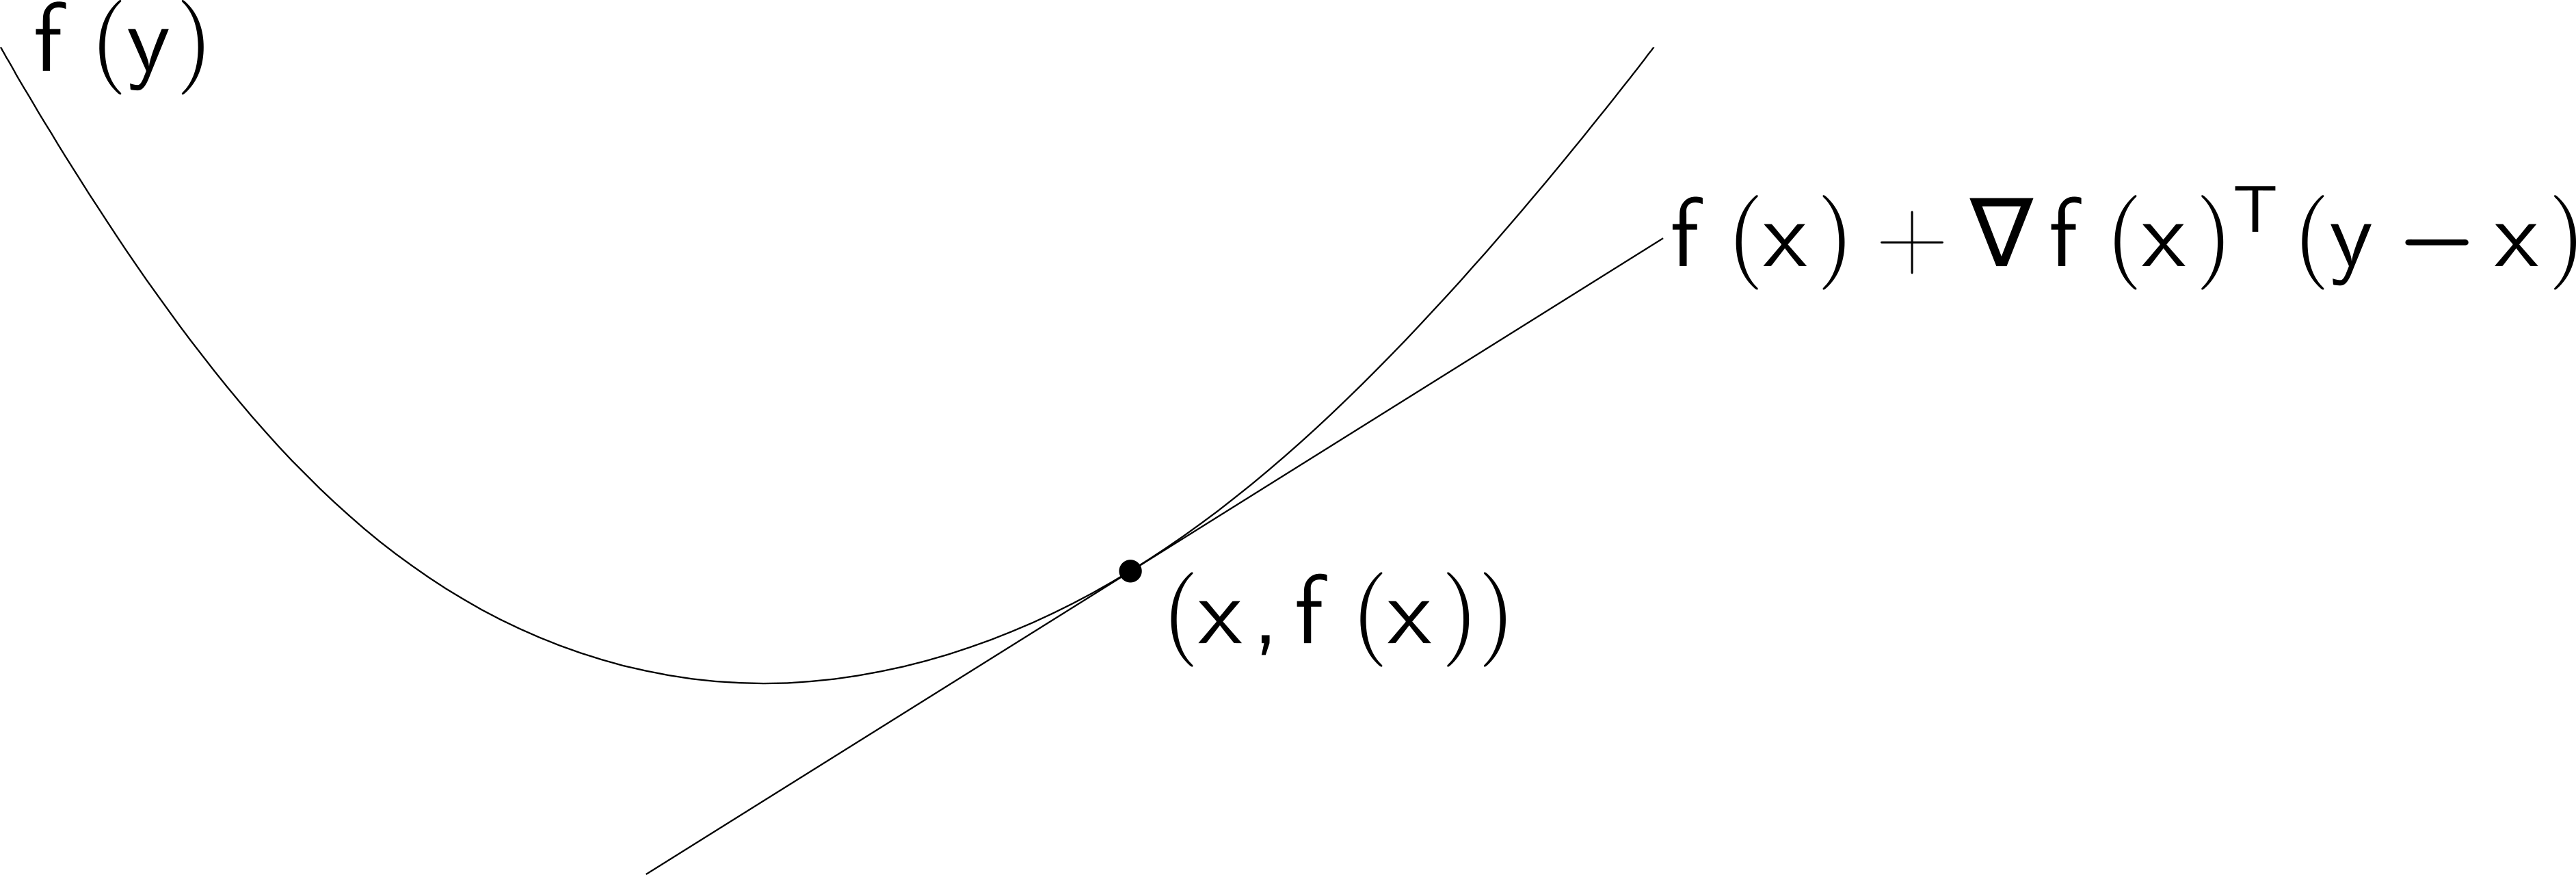
\includegraphics[width=.5\textwidth]{../Graphics/069.png}\hfil

\clearpage
\hfil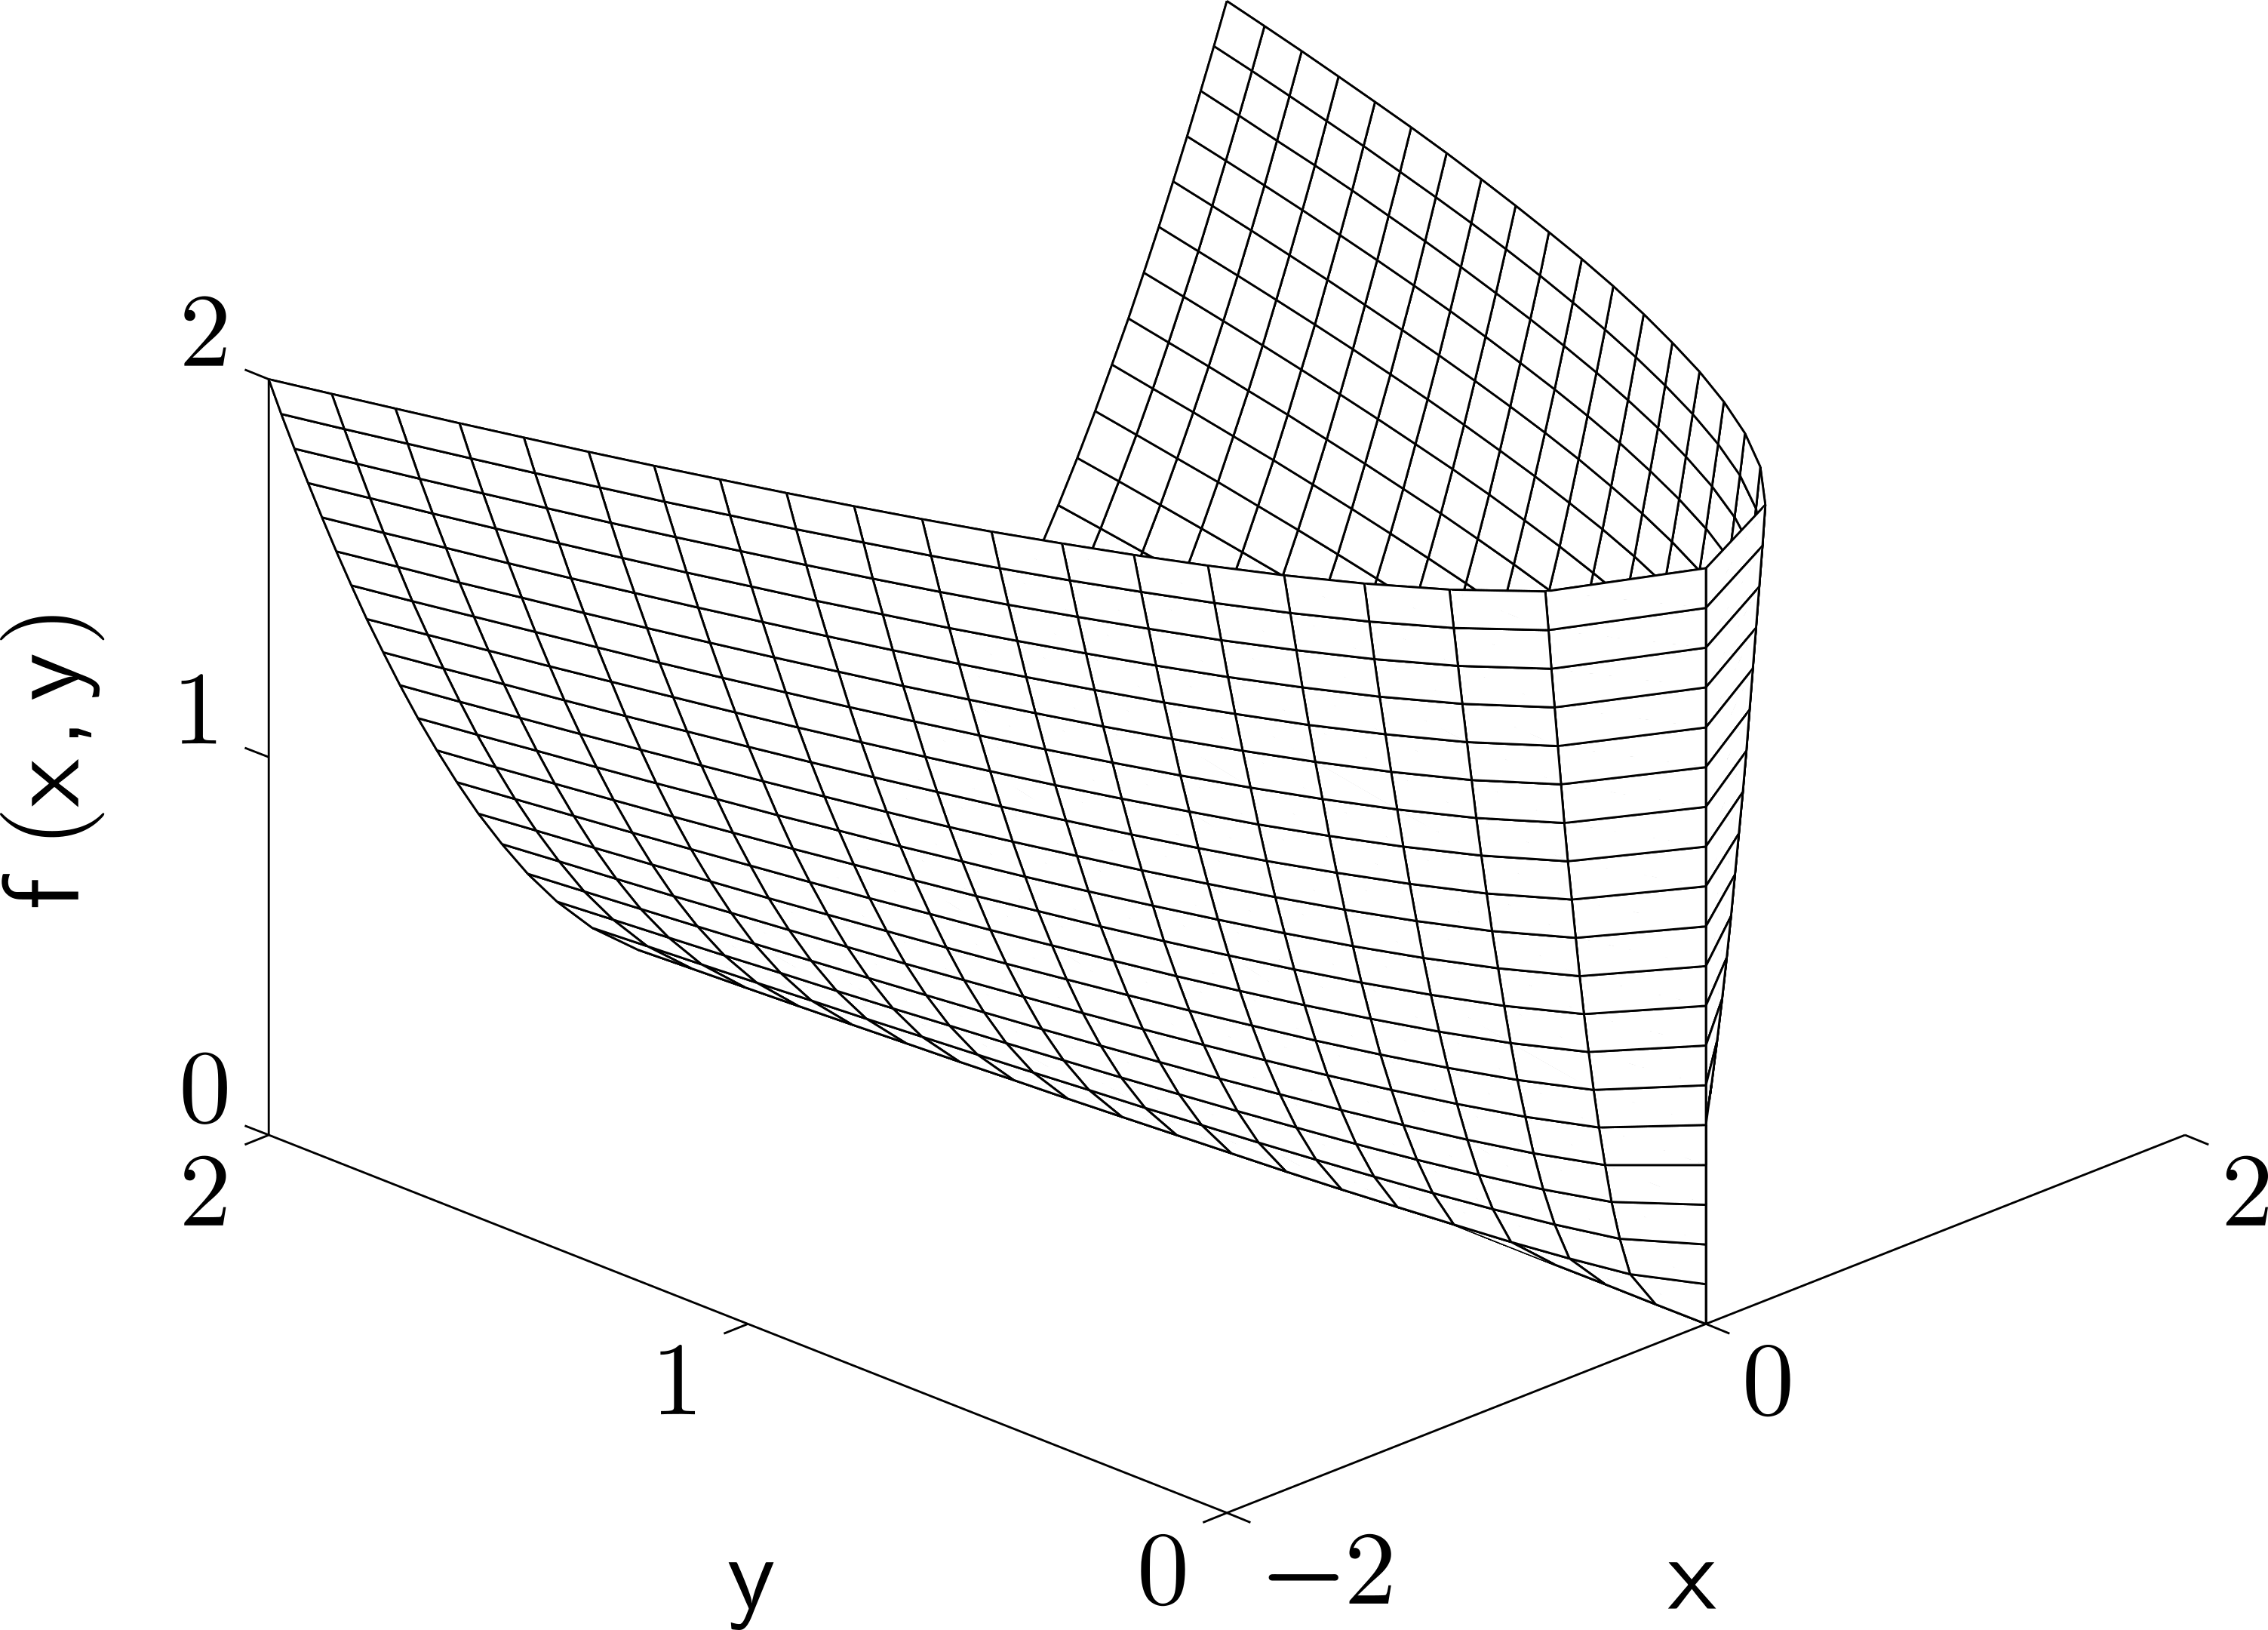
\includegraphics[width=.5\textwidth]{../Graphics/072.png}\hfil

\clearpage
\hfil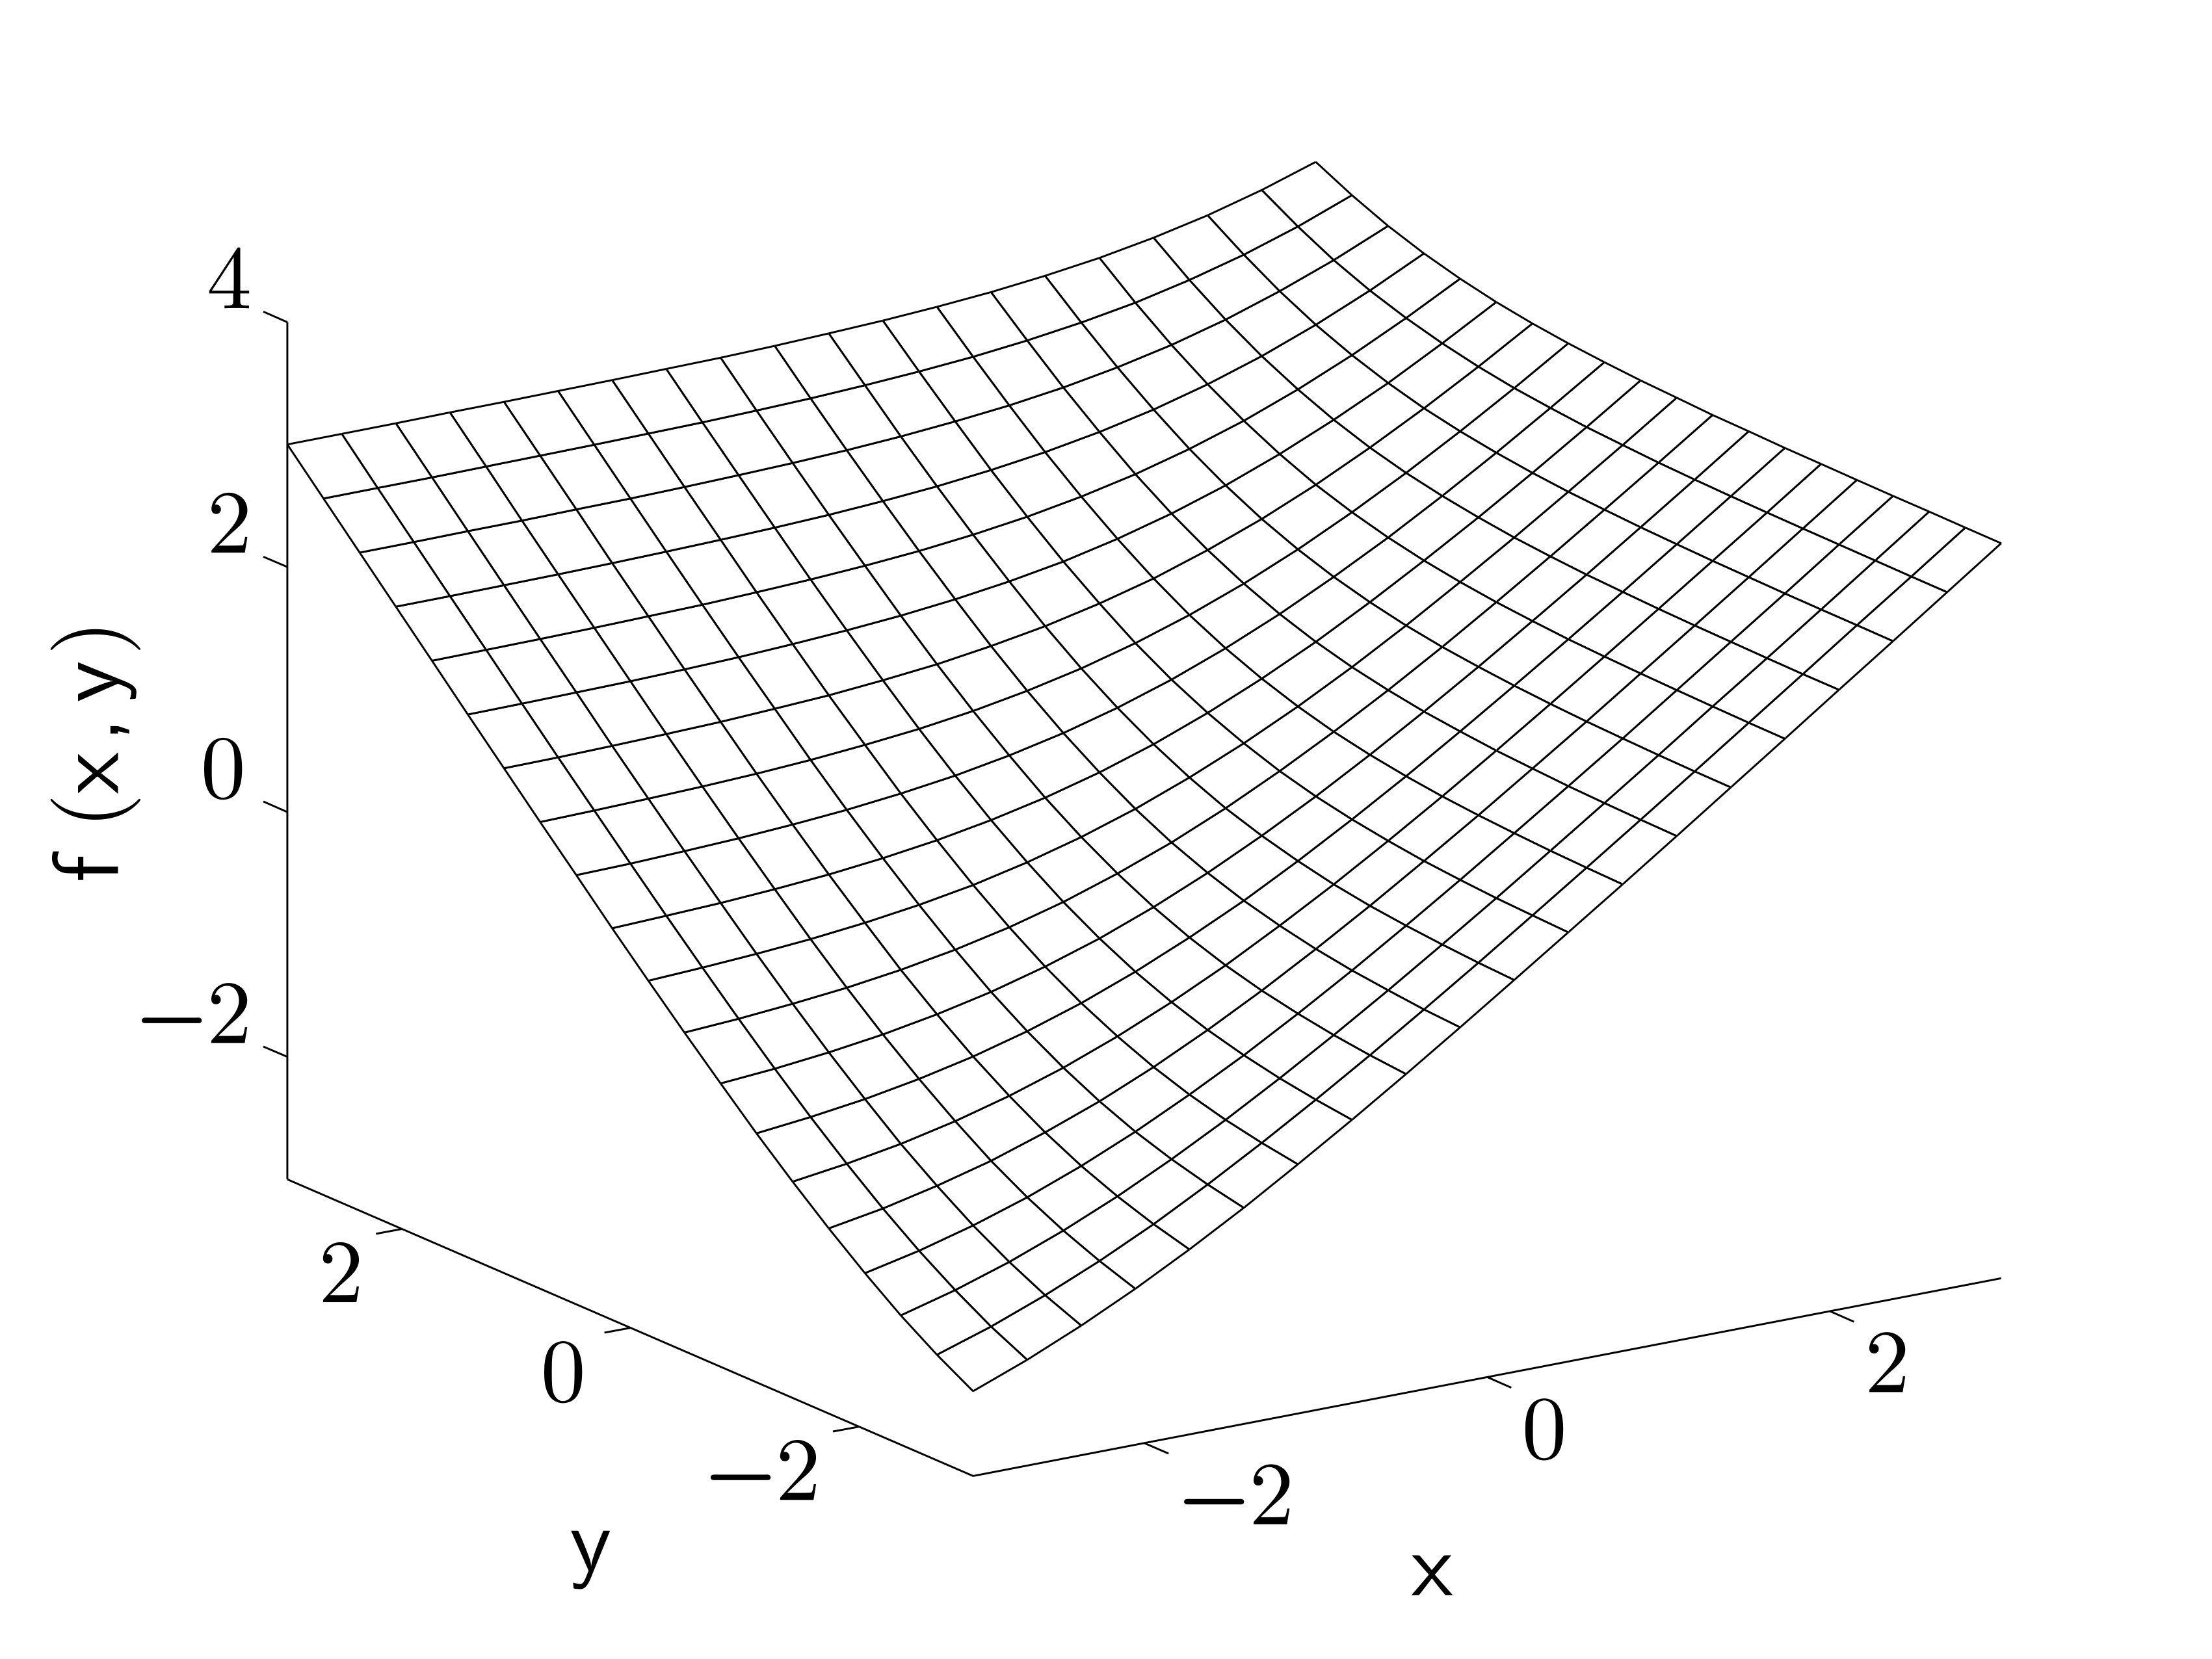
\includegraphics[width=.5\textwidth]{../Graphics/073.png}\hfil

\clearpage
\hfil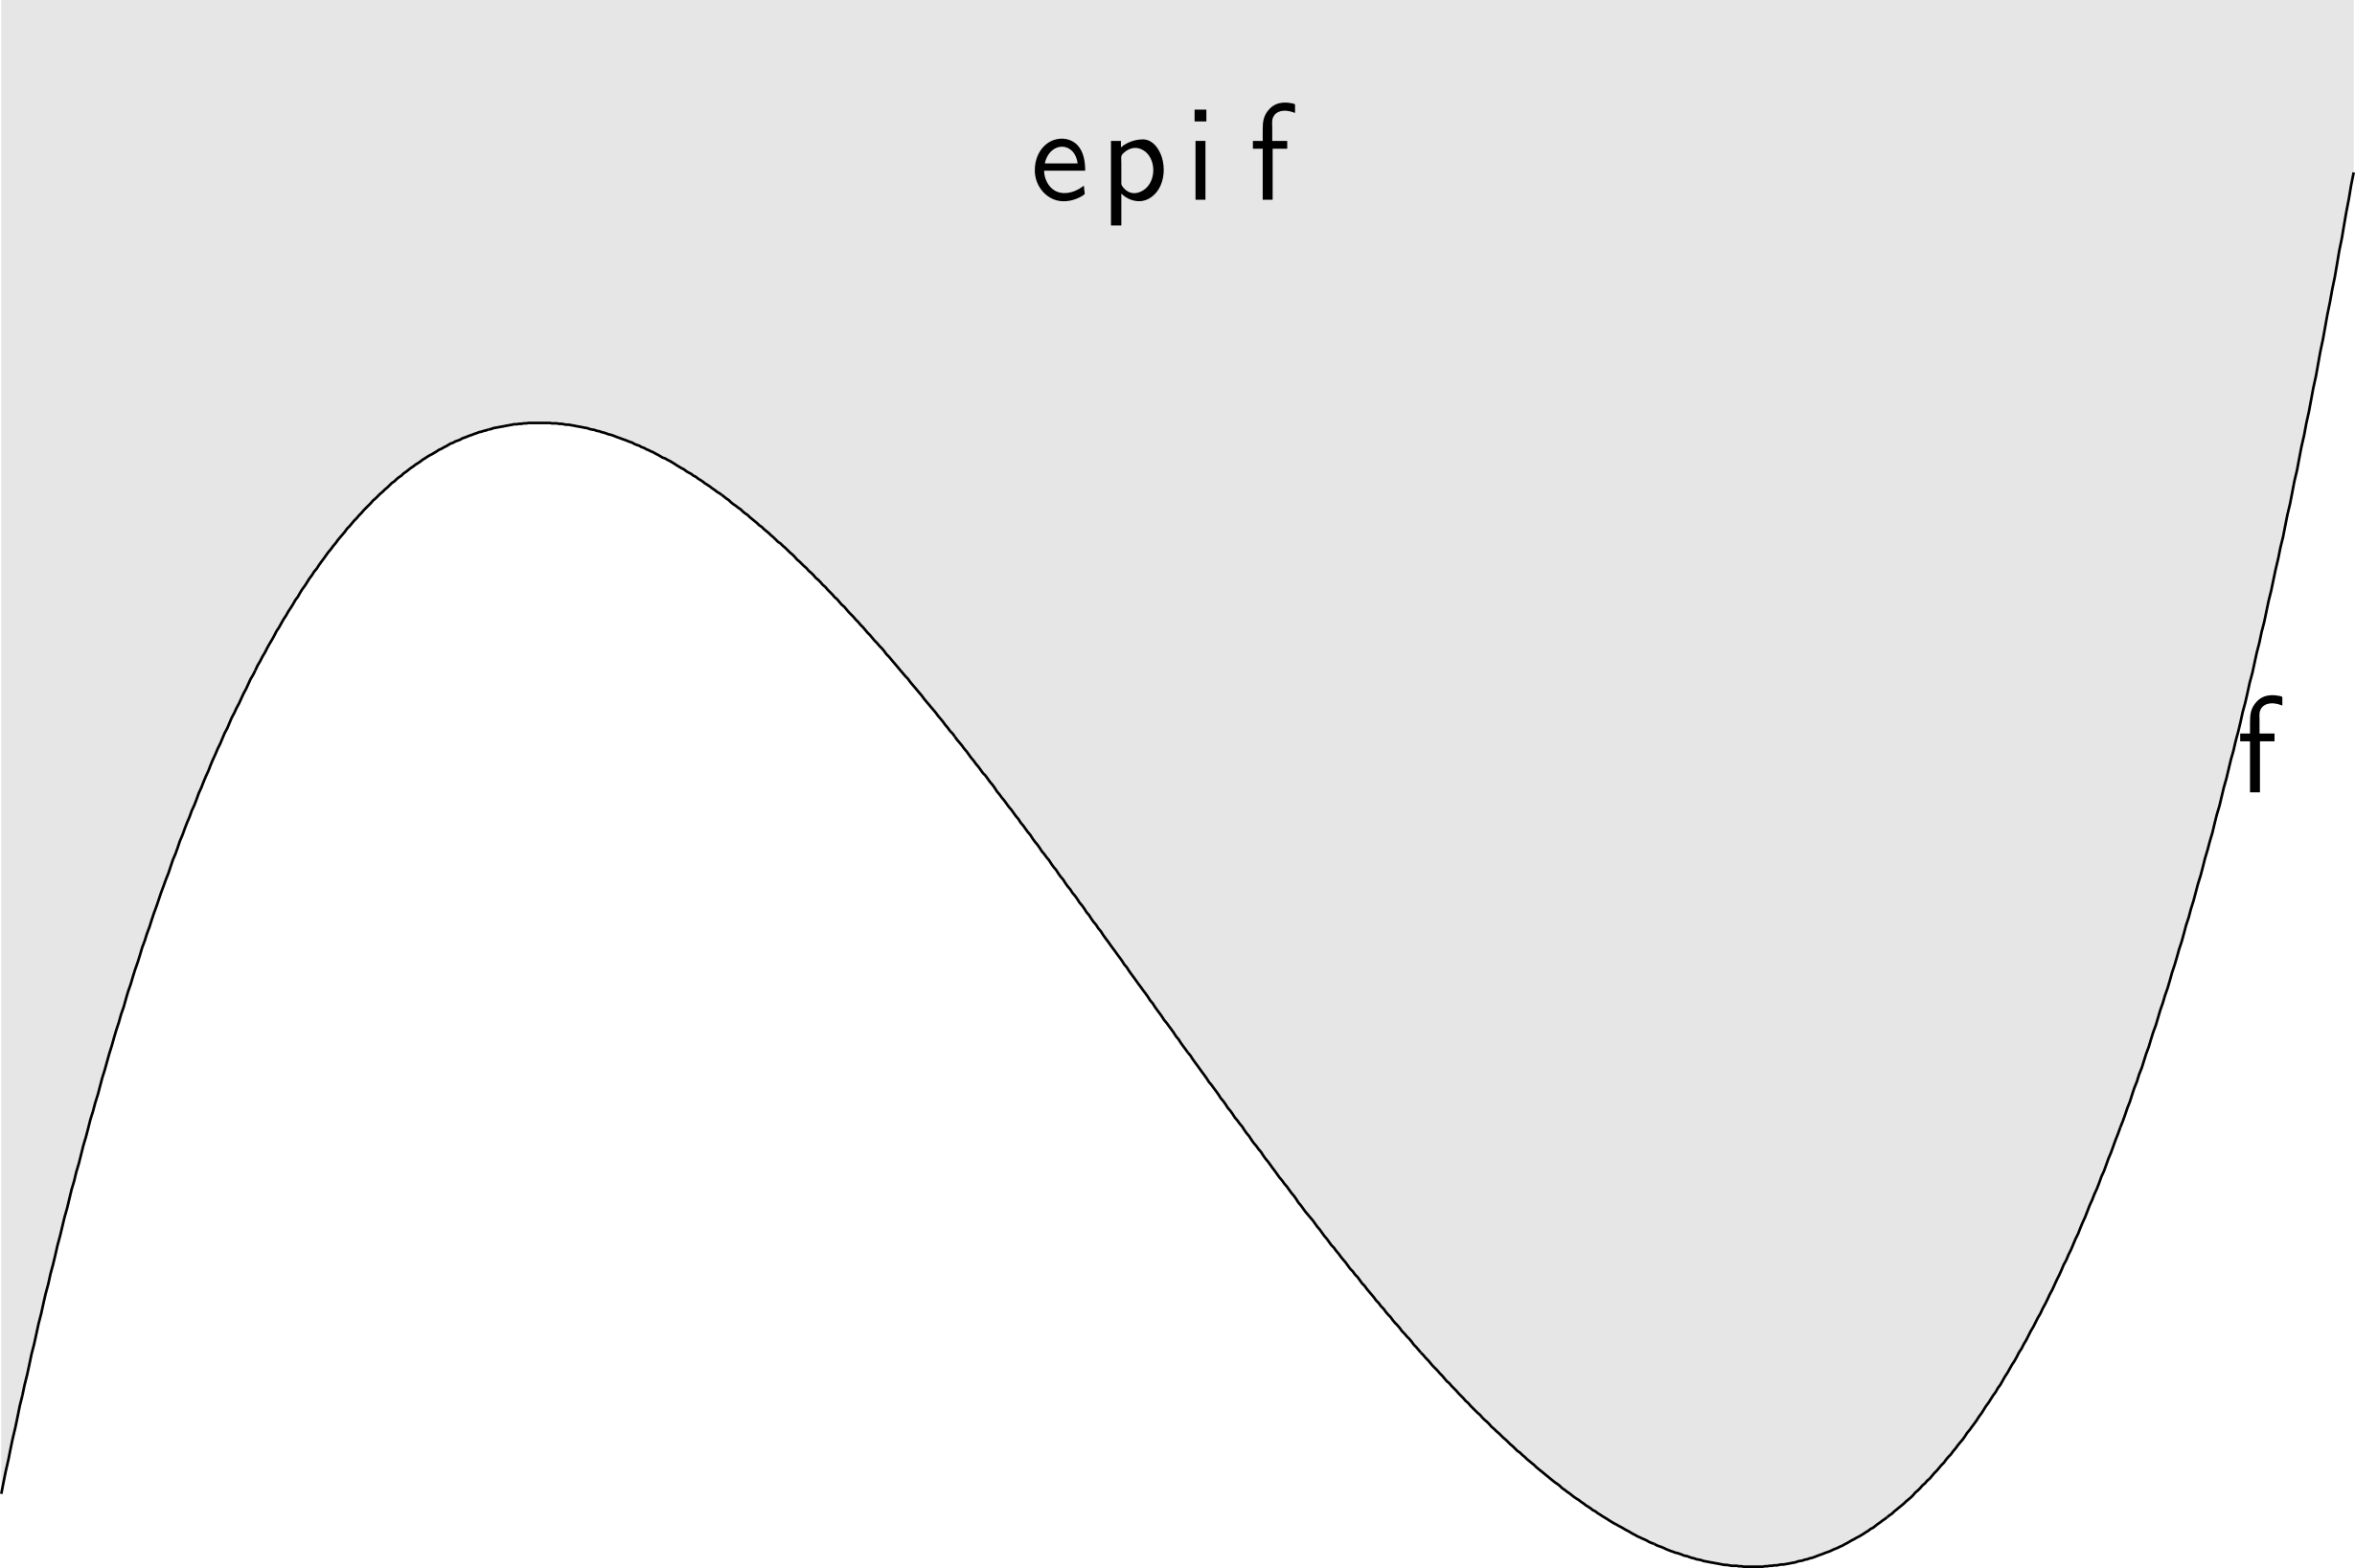
\includegraphics[width=.5\textwidth]{../Graphics/076.png}\hfil

\clearpage
\hfil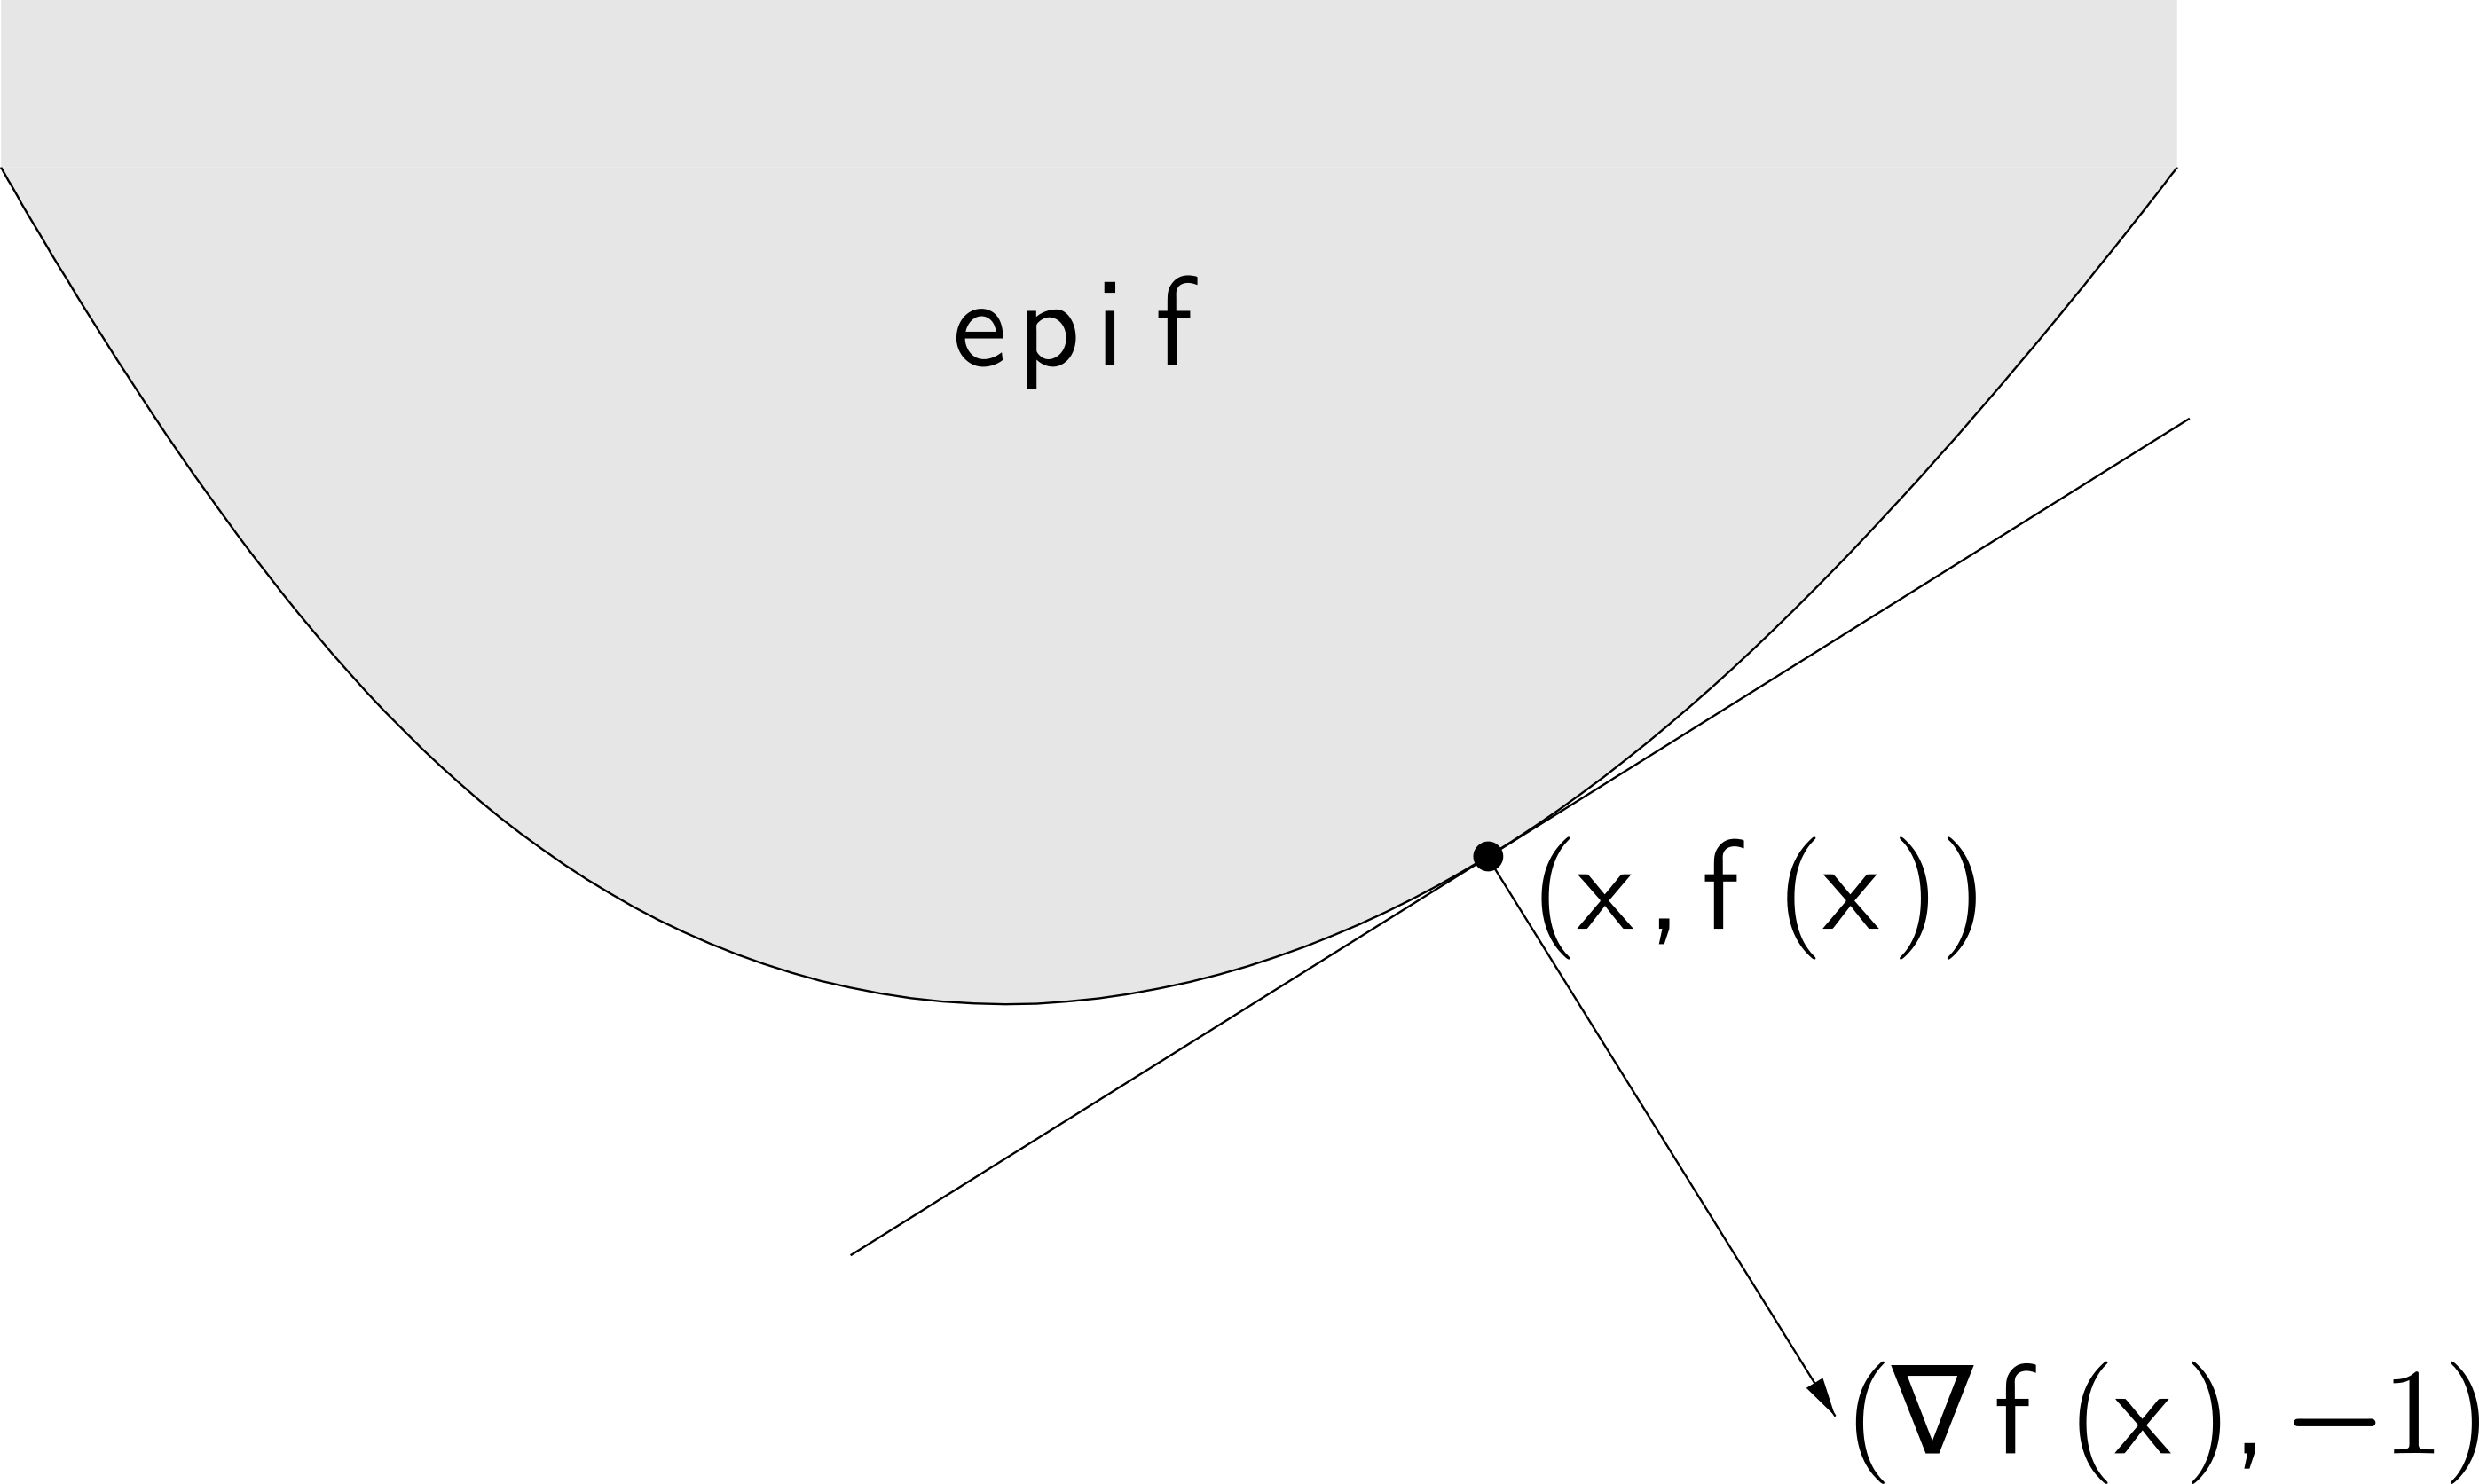
\includegraphics[width=.5\textwidth]{../Graphics/077.png}\hfil

\clearpage
\hfil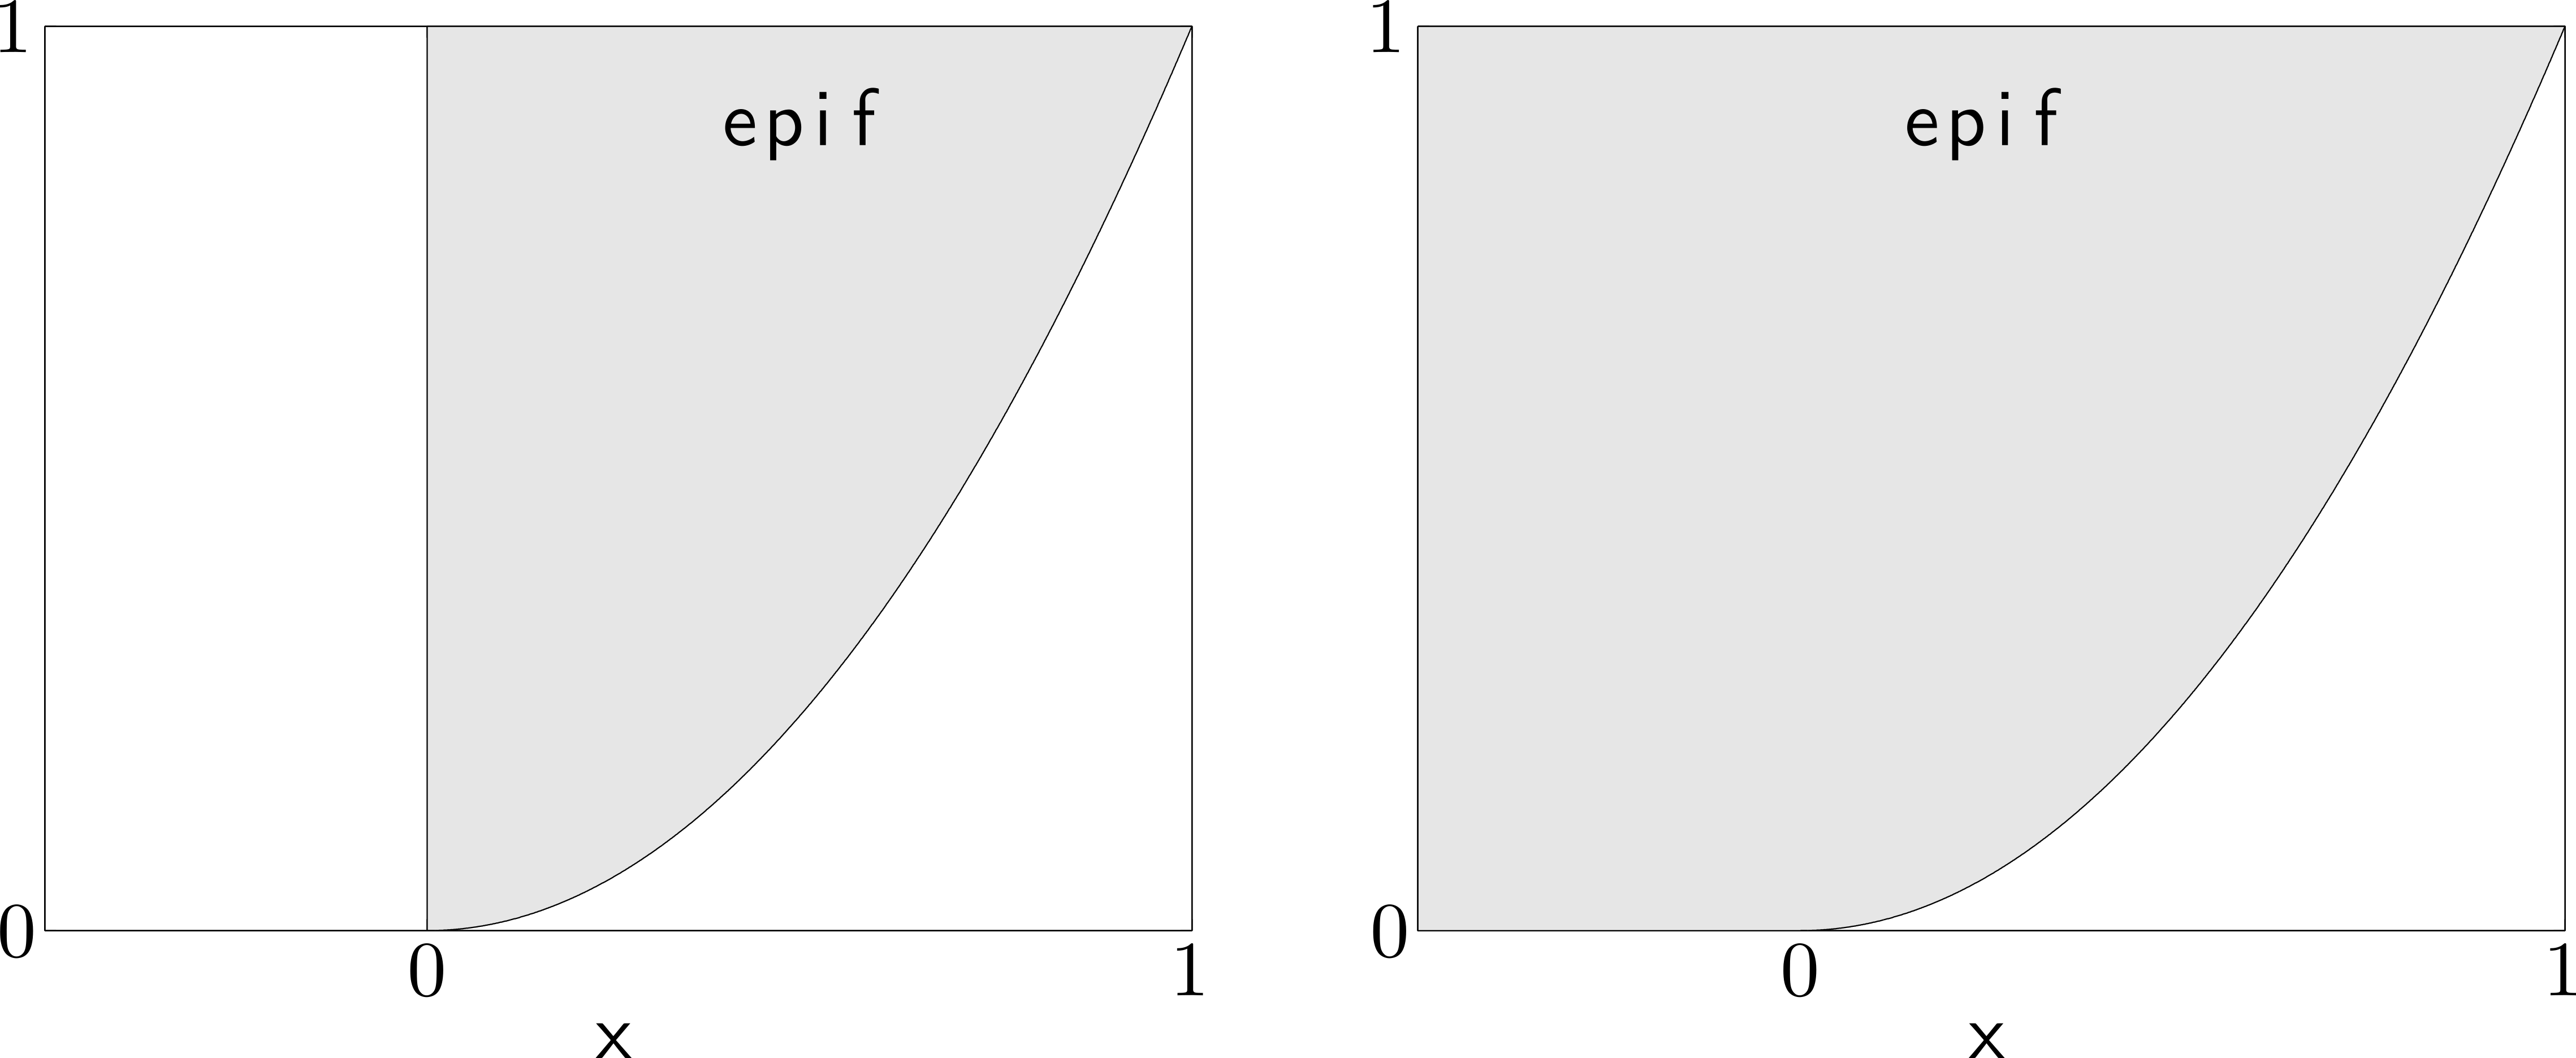
\includegraphics[width=.5\textwidth]{../Graphics/085.png}\hfil

\clearpage
\hfil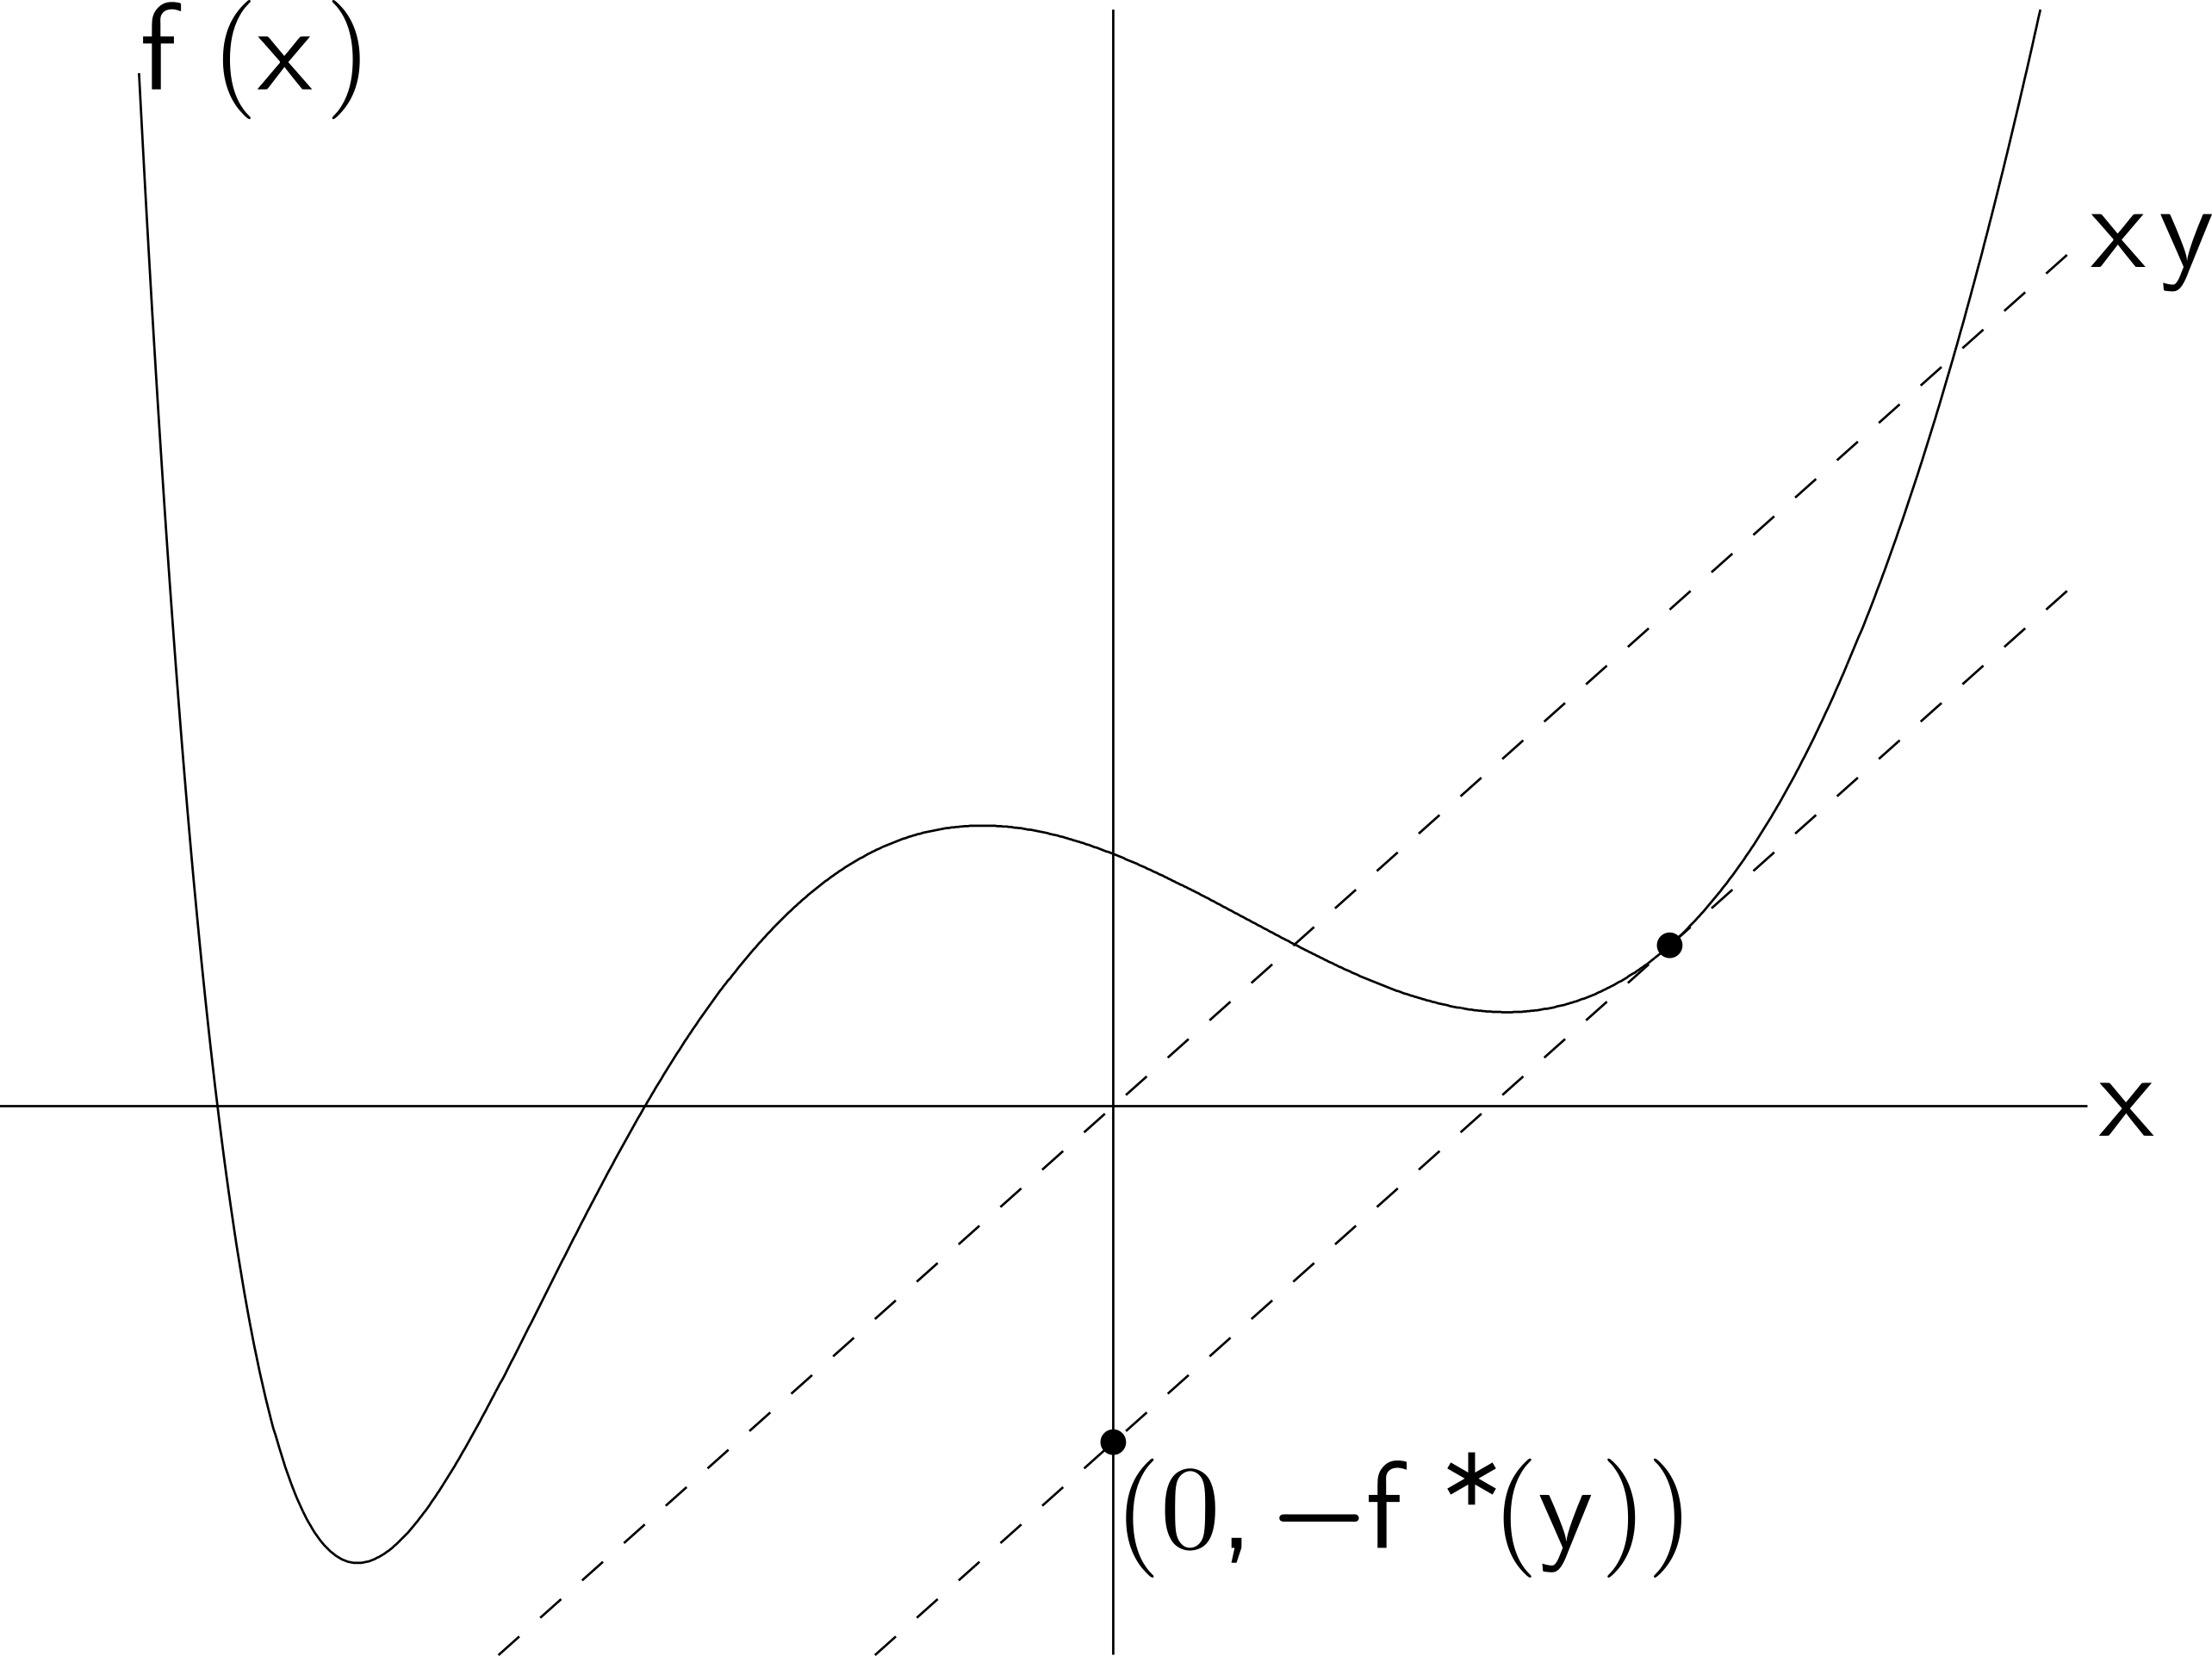
\includegraphics[width=.5\textwidth]{../Graphics/091.png}\hfil

\clearpage
\hfil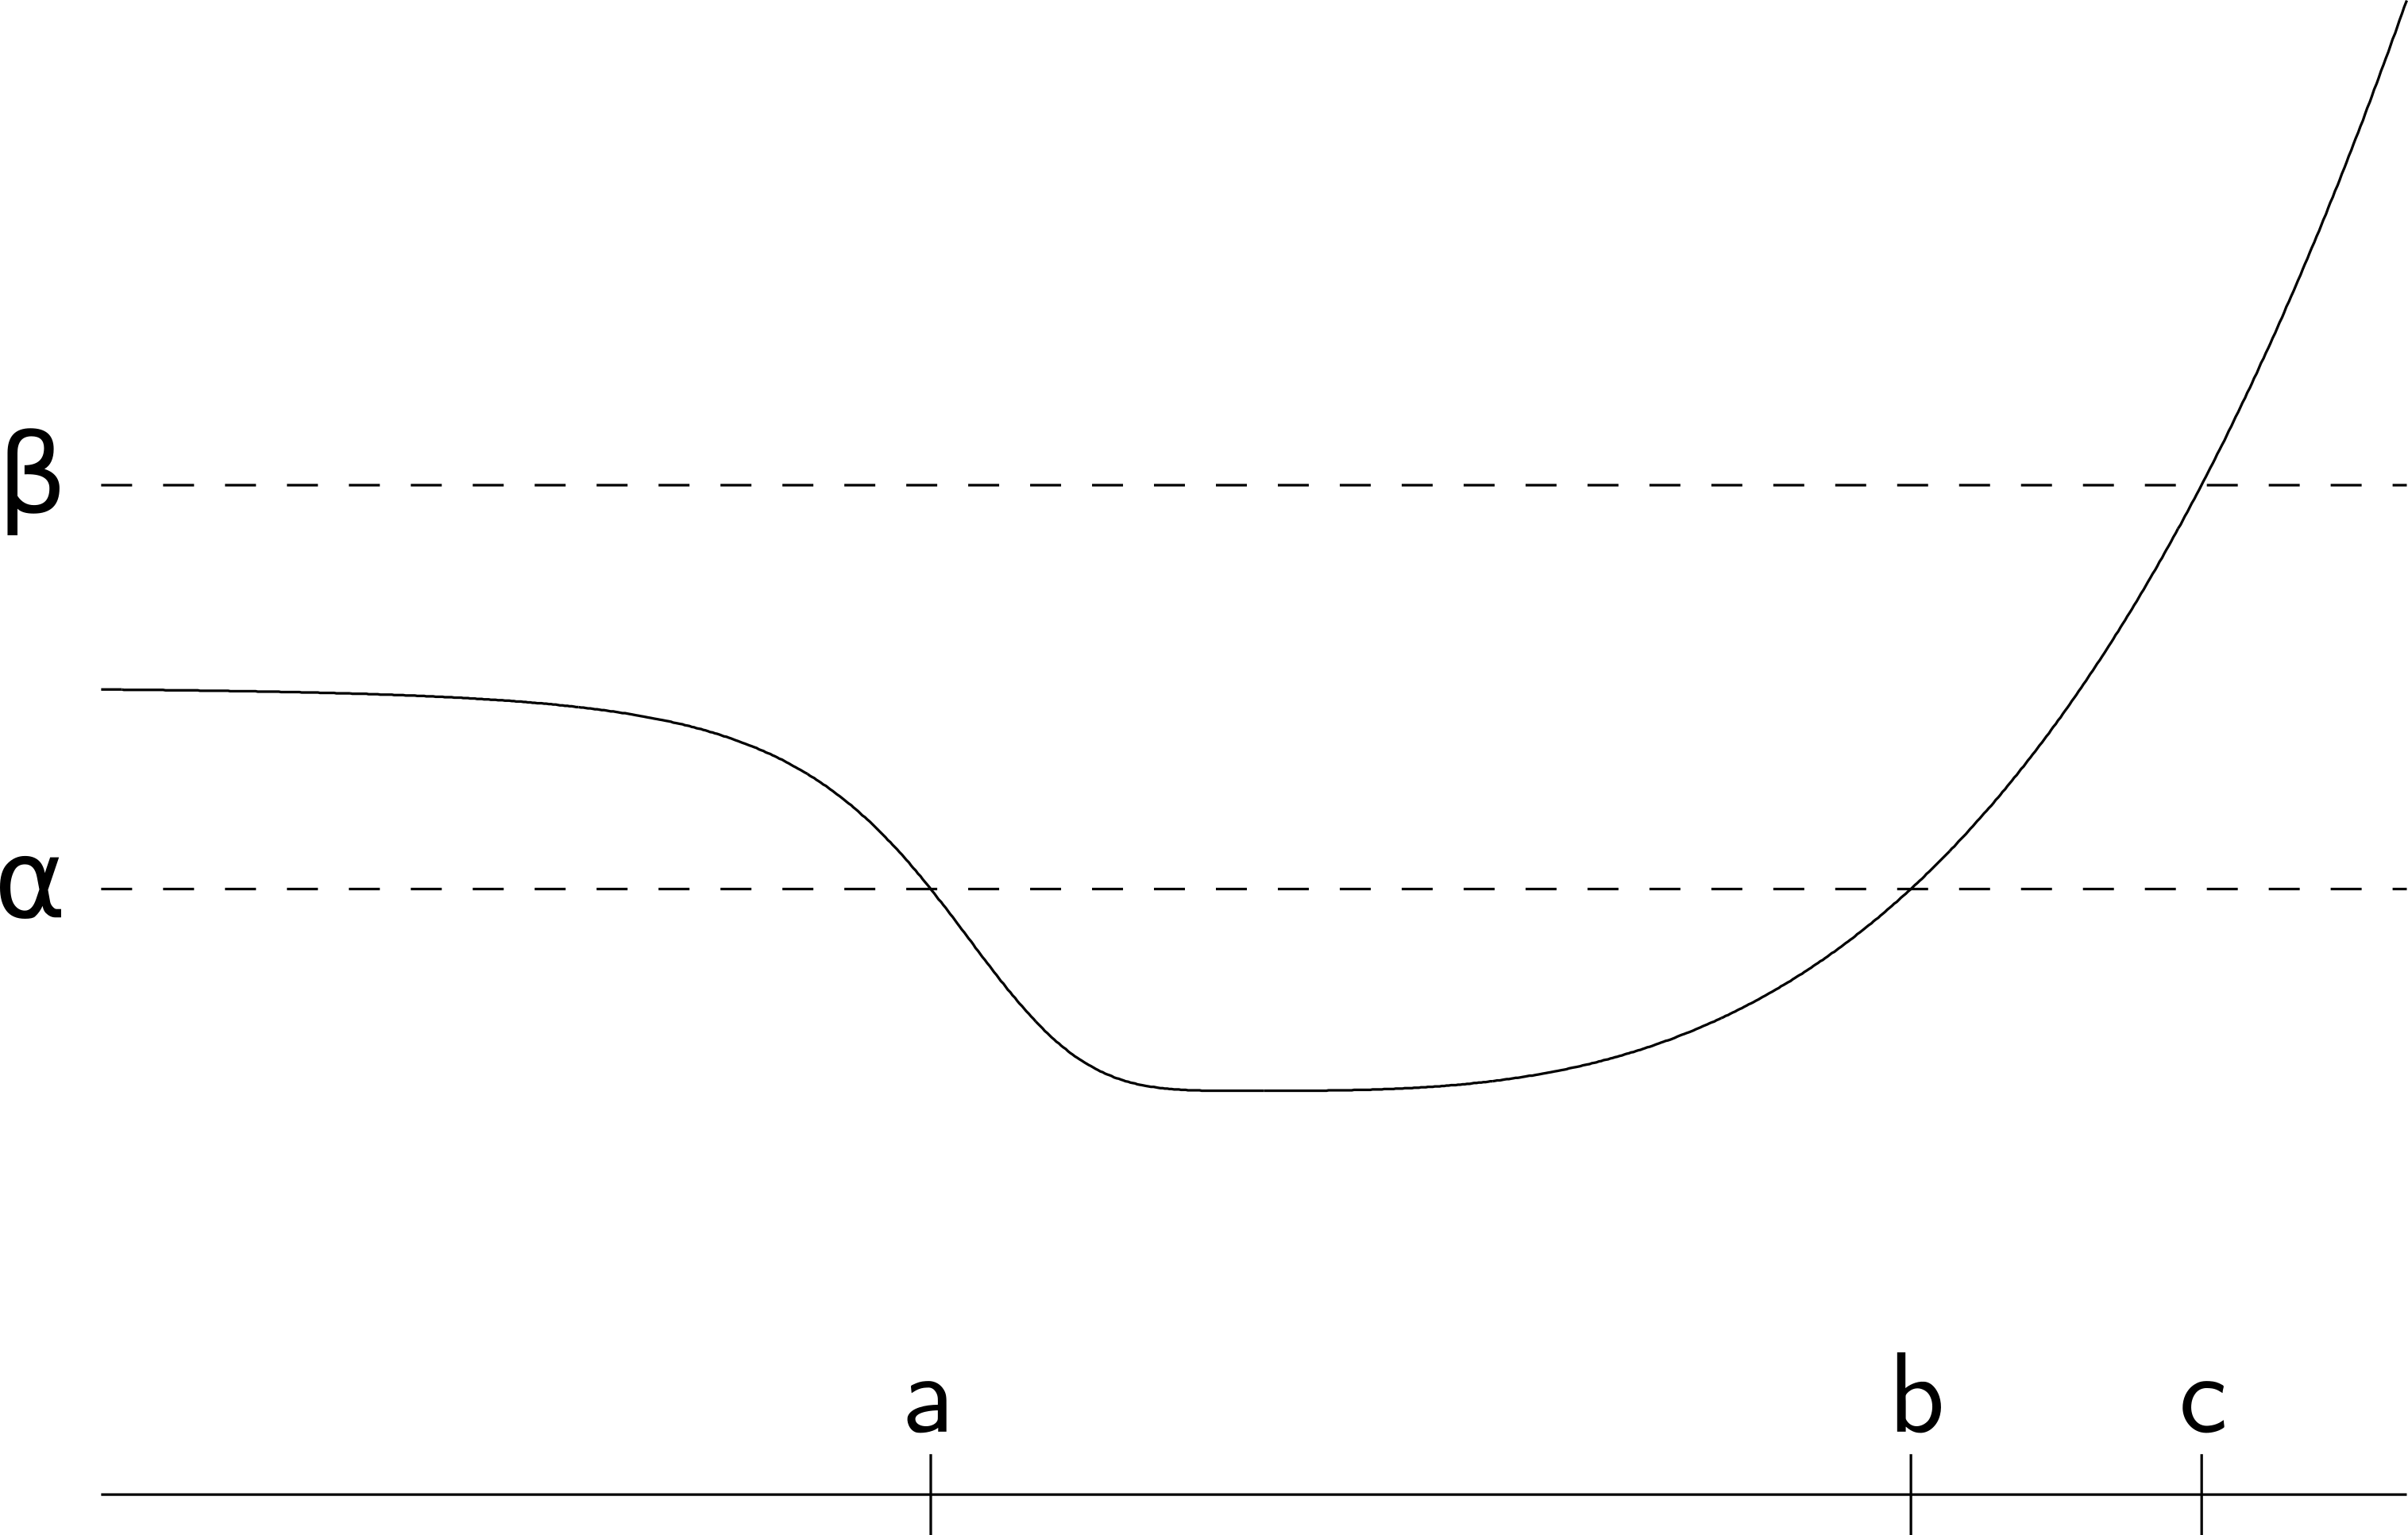
\includegraphics[width=.5\textwidth]{../Graphics/096.png}\hfil

\clearpage
\hfil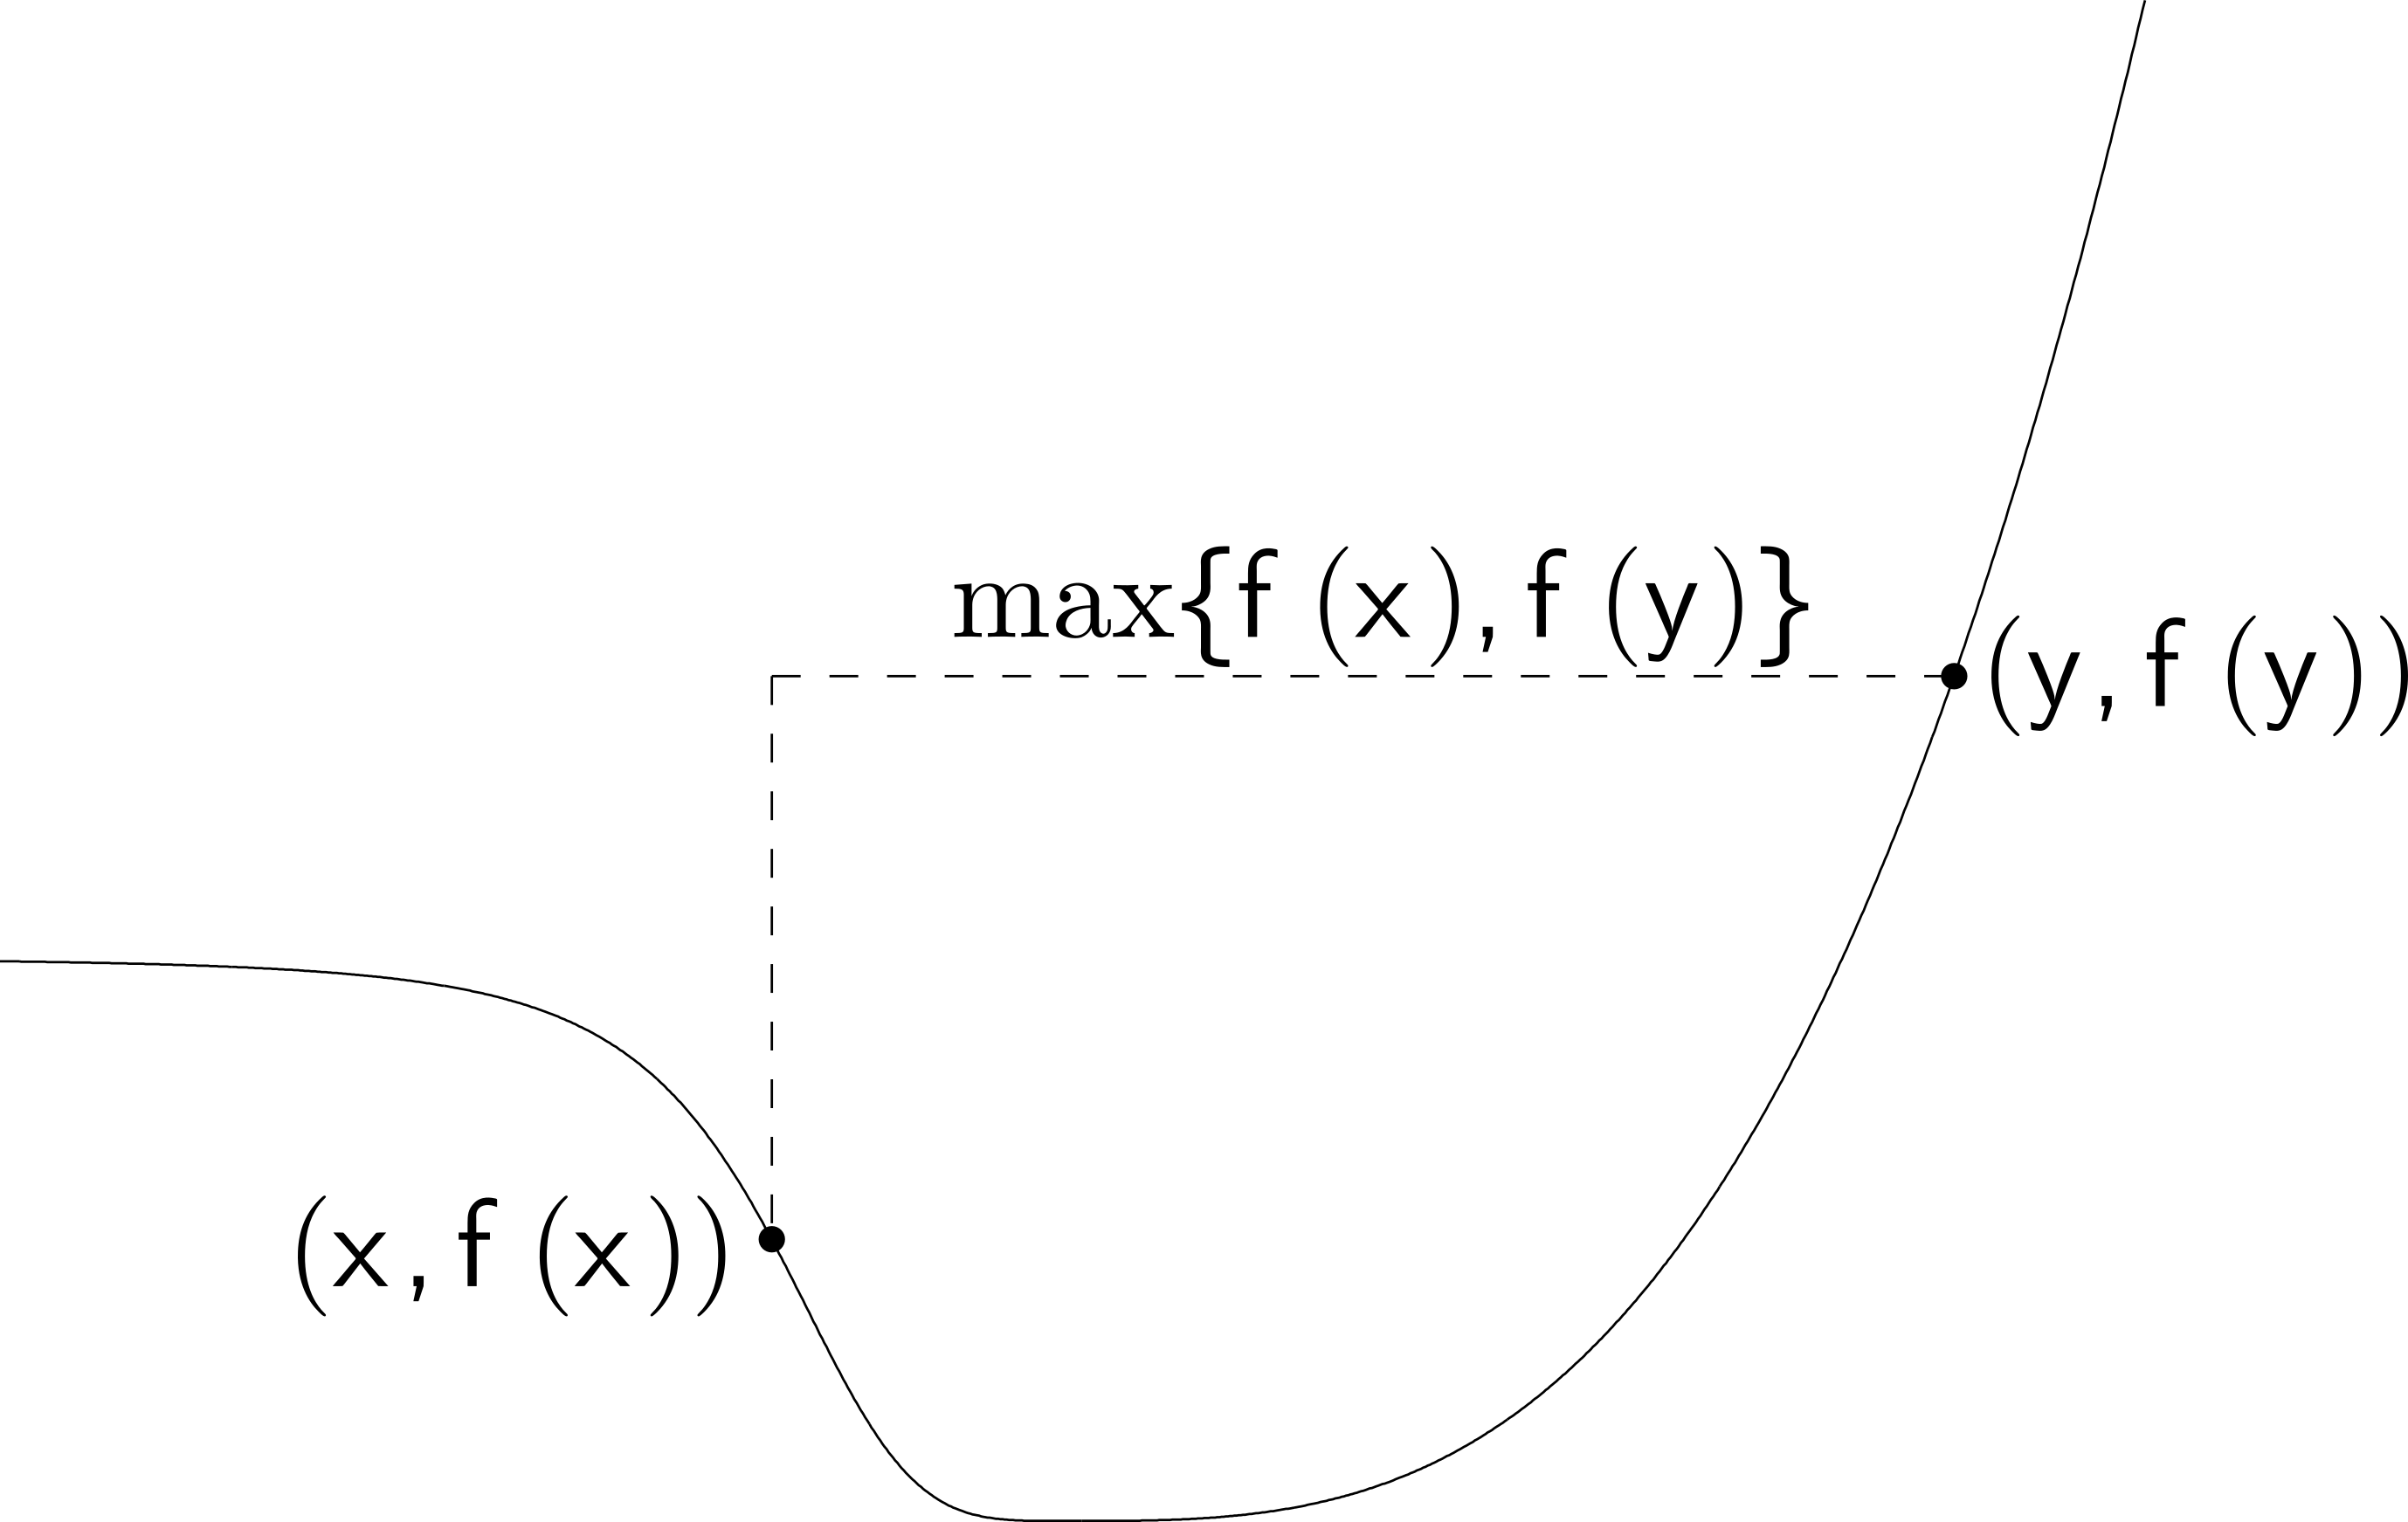
\includegraphics[width=.5\textwidth]{../Graphics/099.png}\hfil

\clearpage
\hfil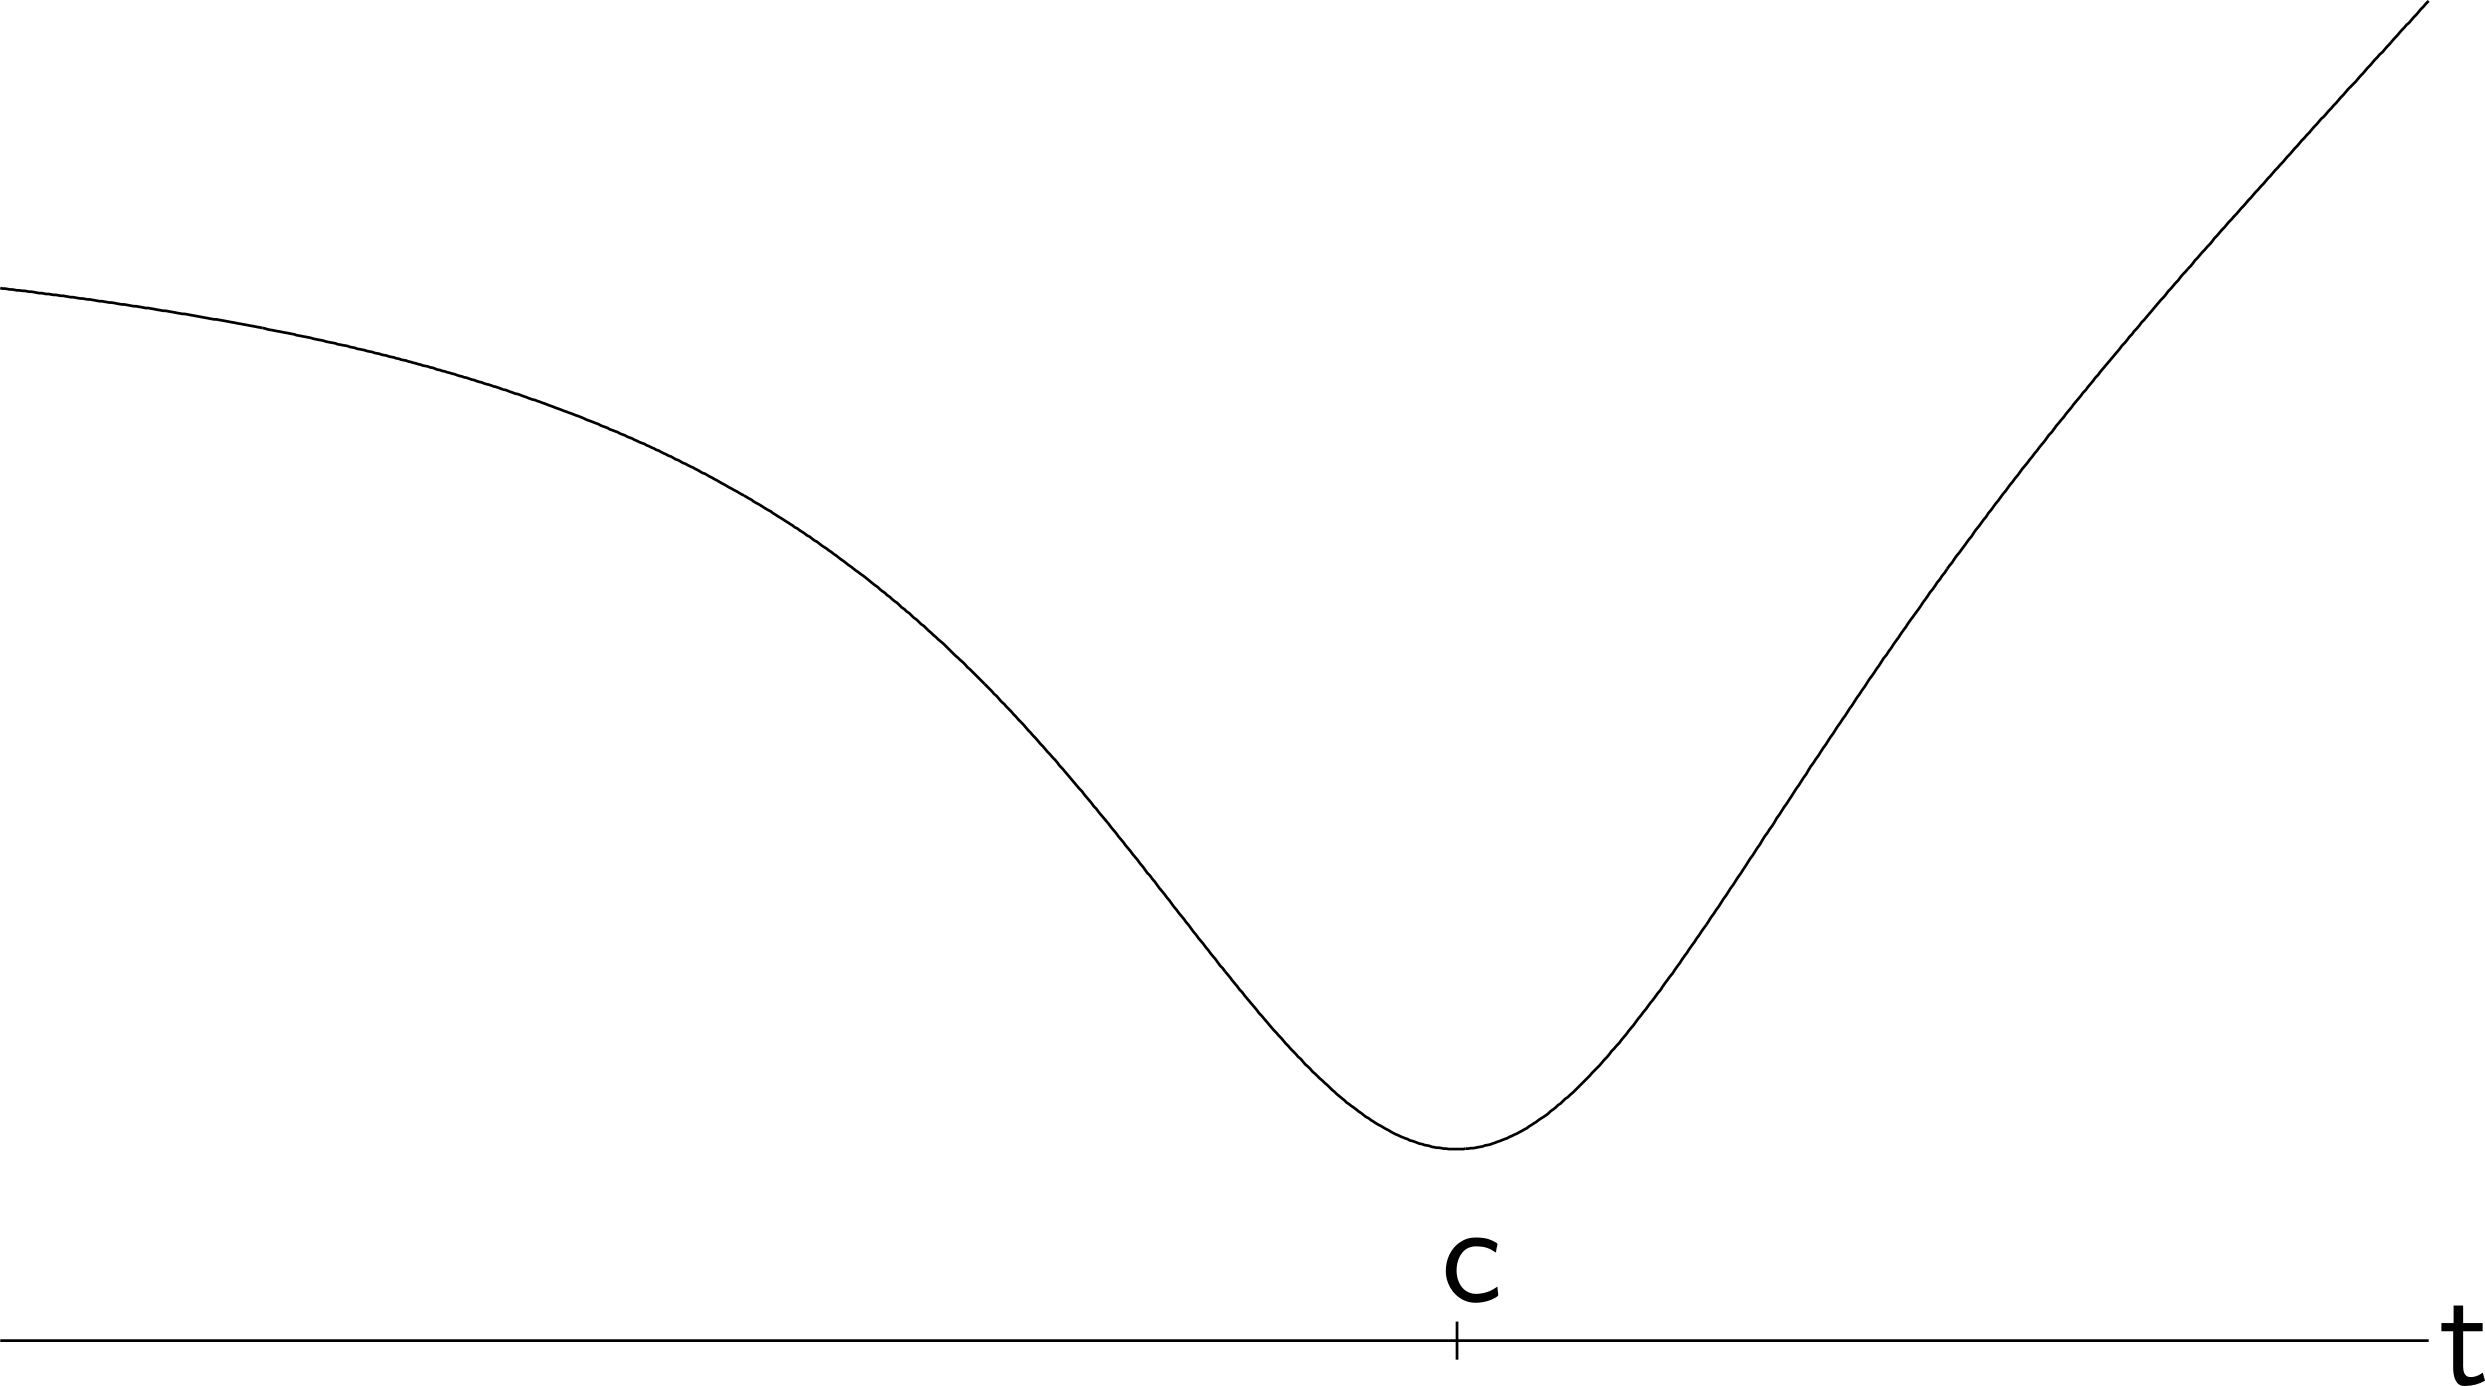
\includegraphics[width=.5\textwidth]{../Graphics/100a.png}\hfil

\clearpage
\hfil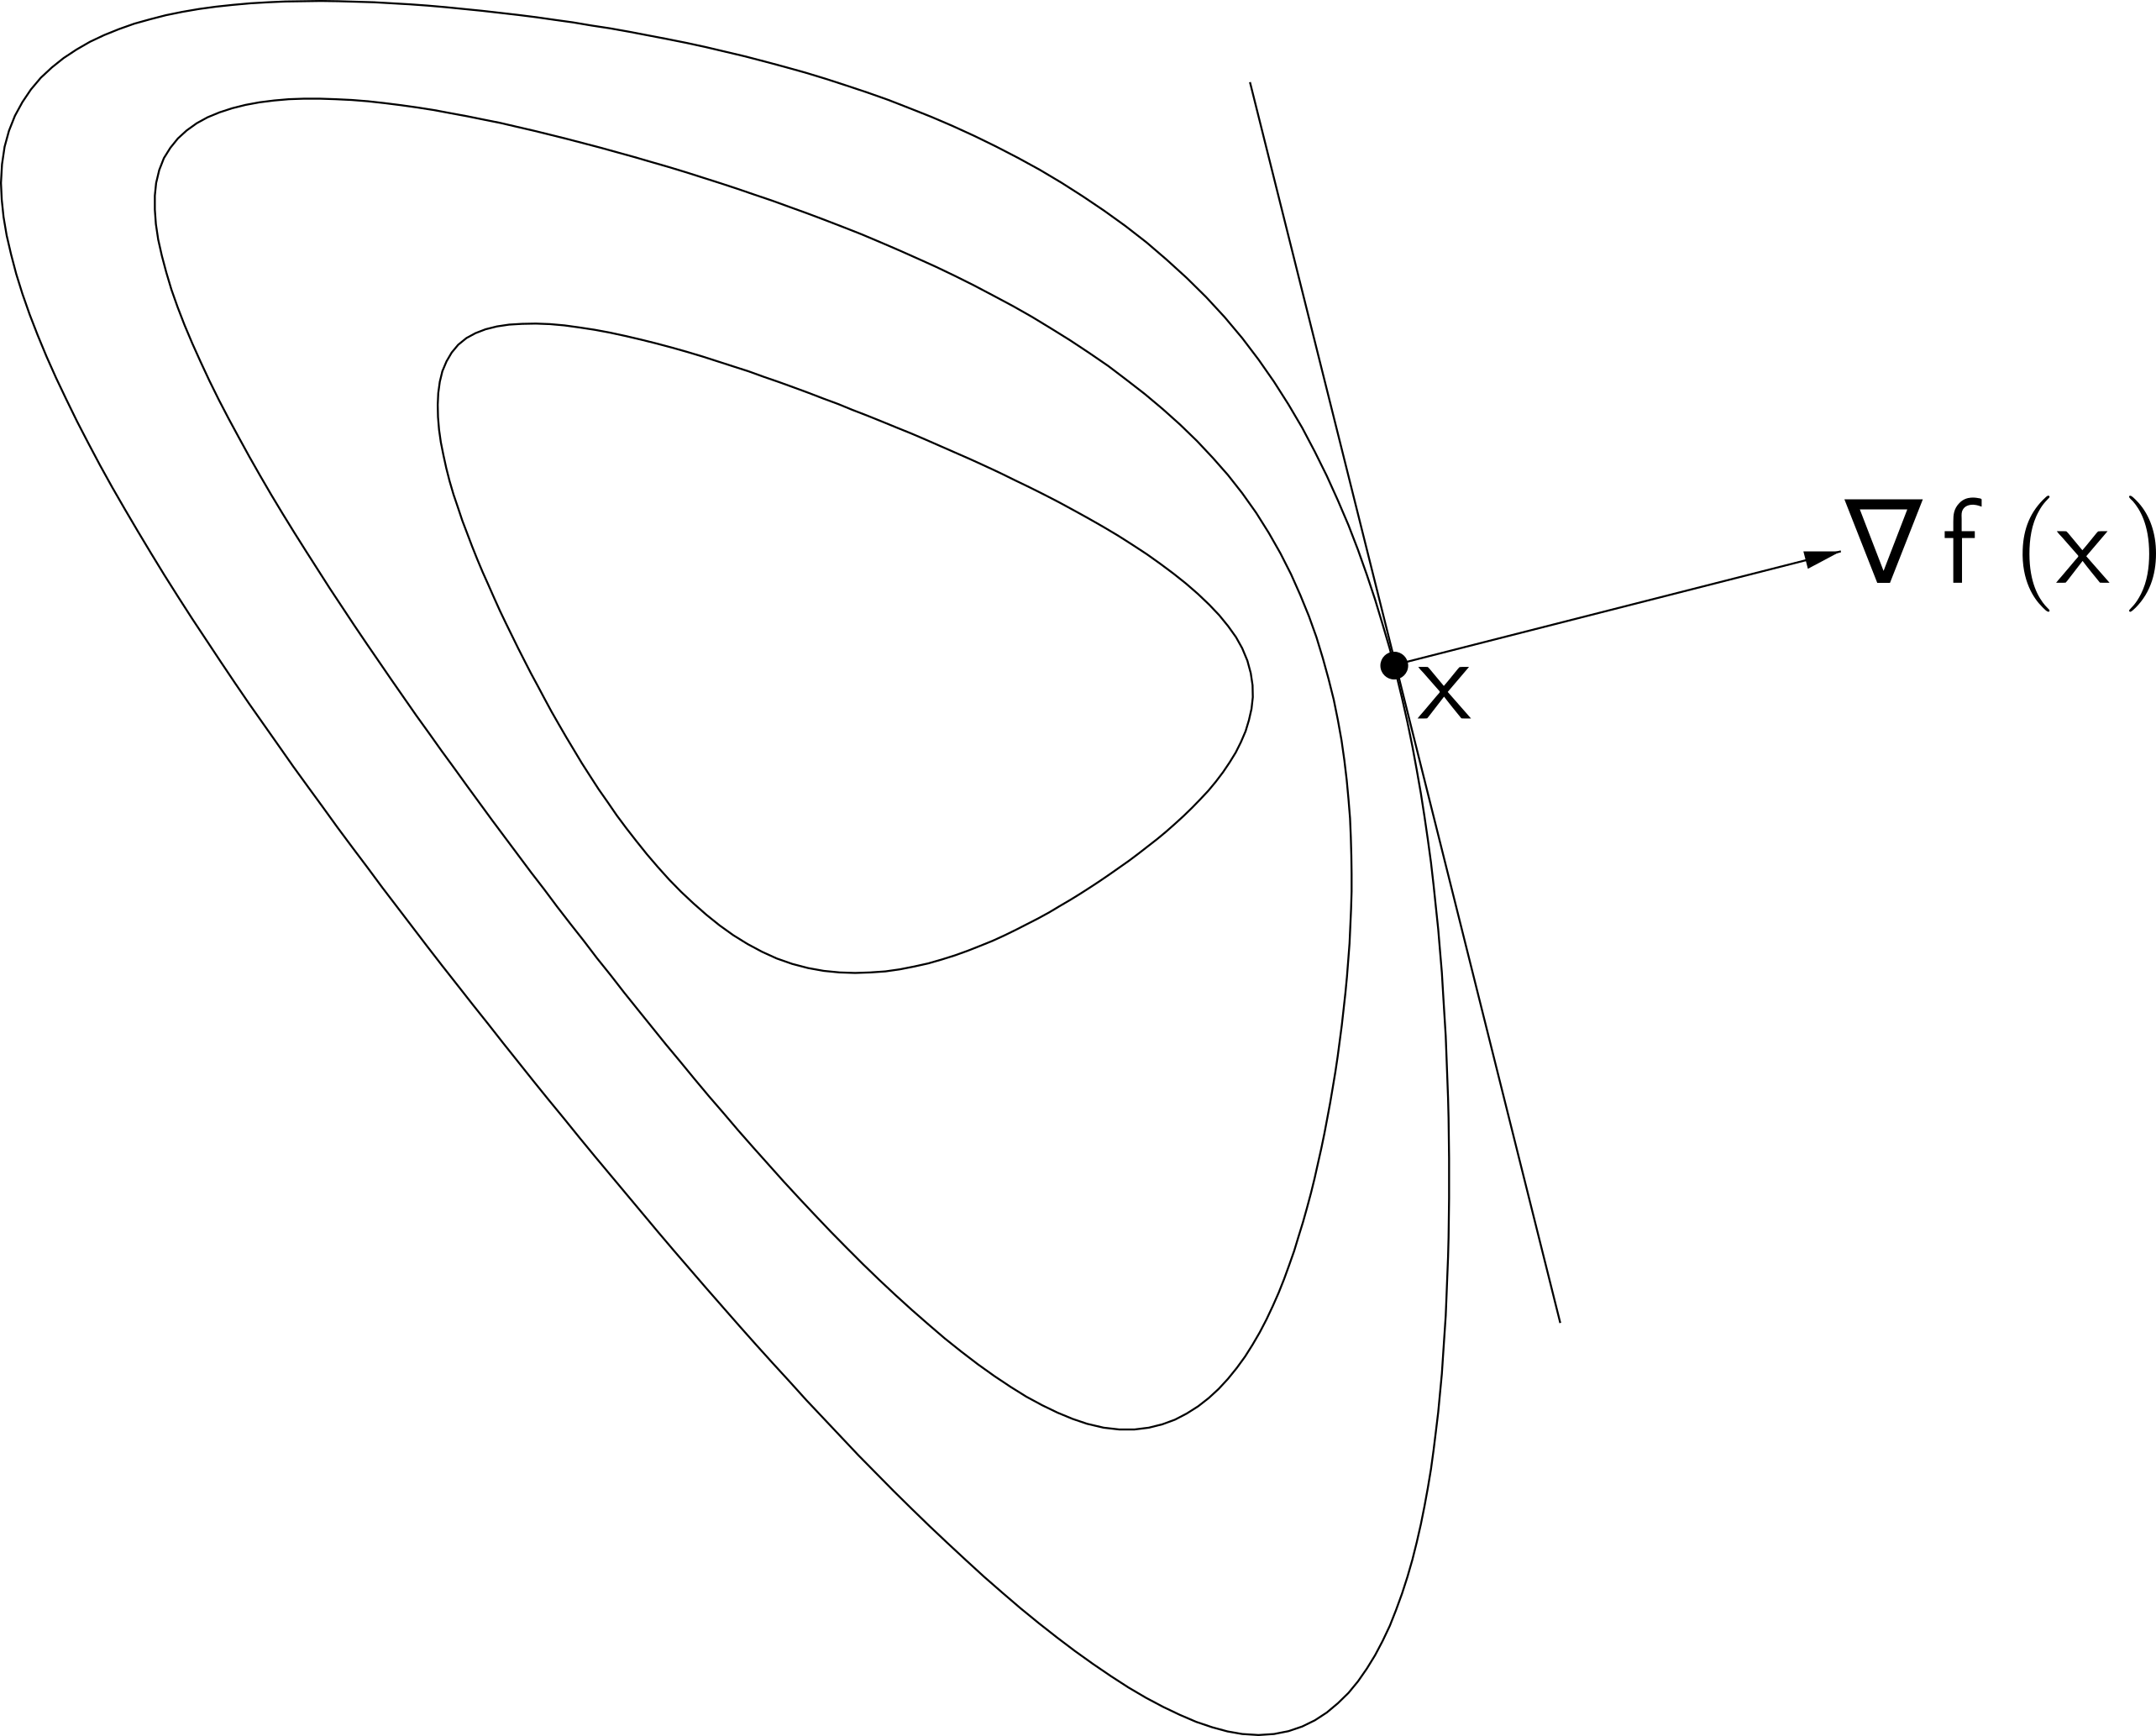
\includegraphics[width=.5\textwidth]{../Graphics/100b.png}\hfil

\clearpage
\hfil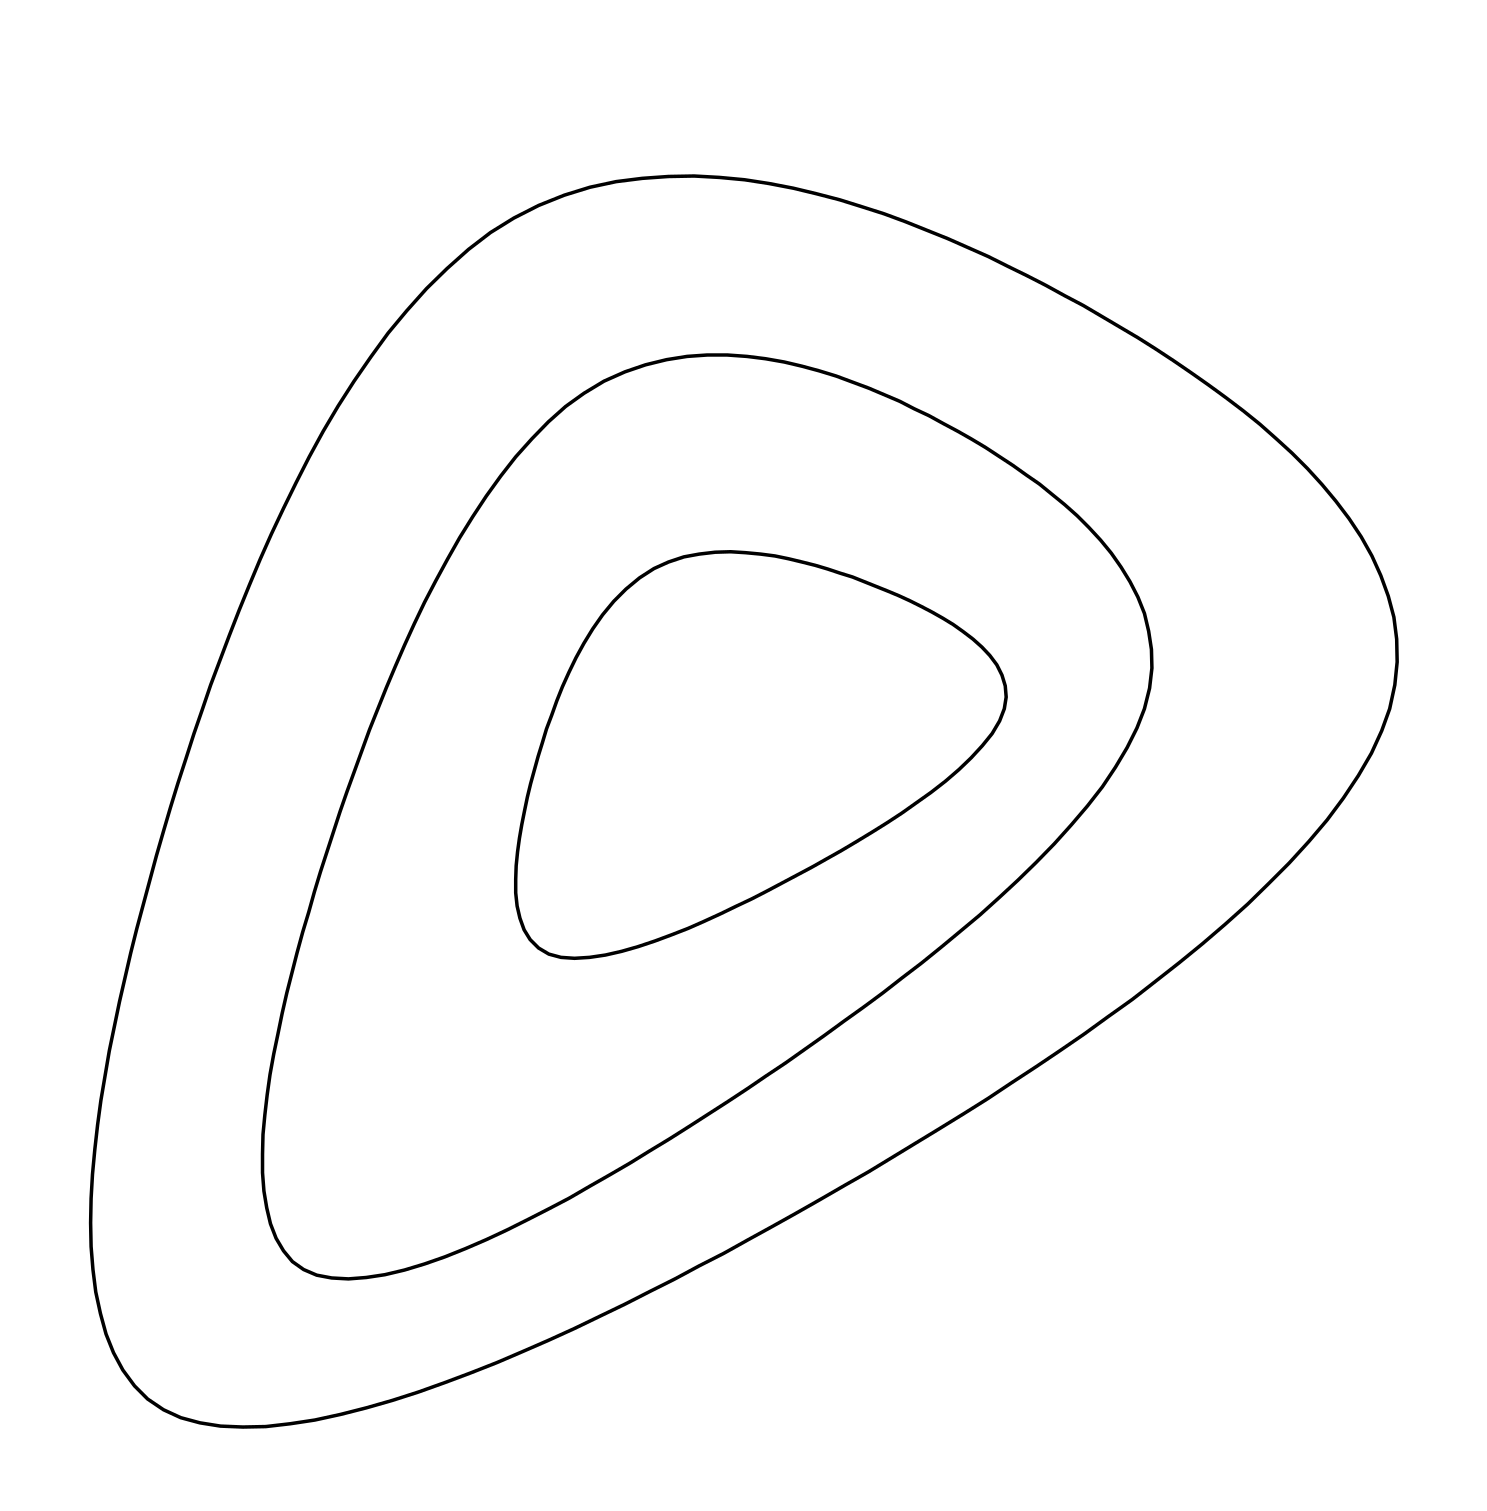
\includegraphics[width=.5\textwidth]{../Graphics/113a.png}\hfil

\clearpage
\hfil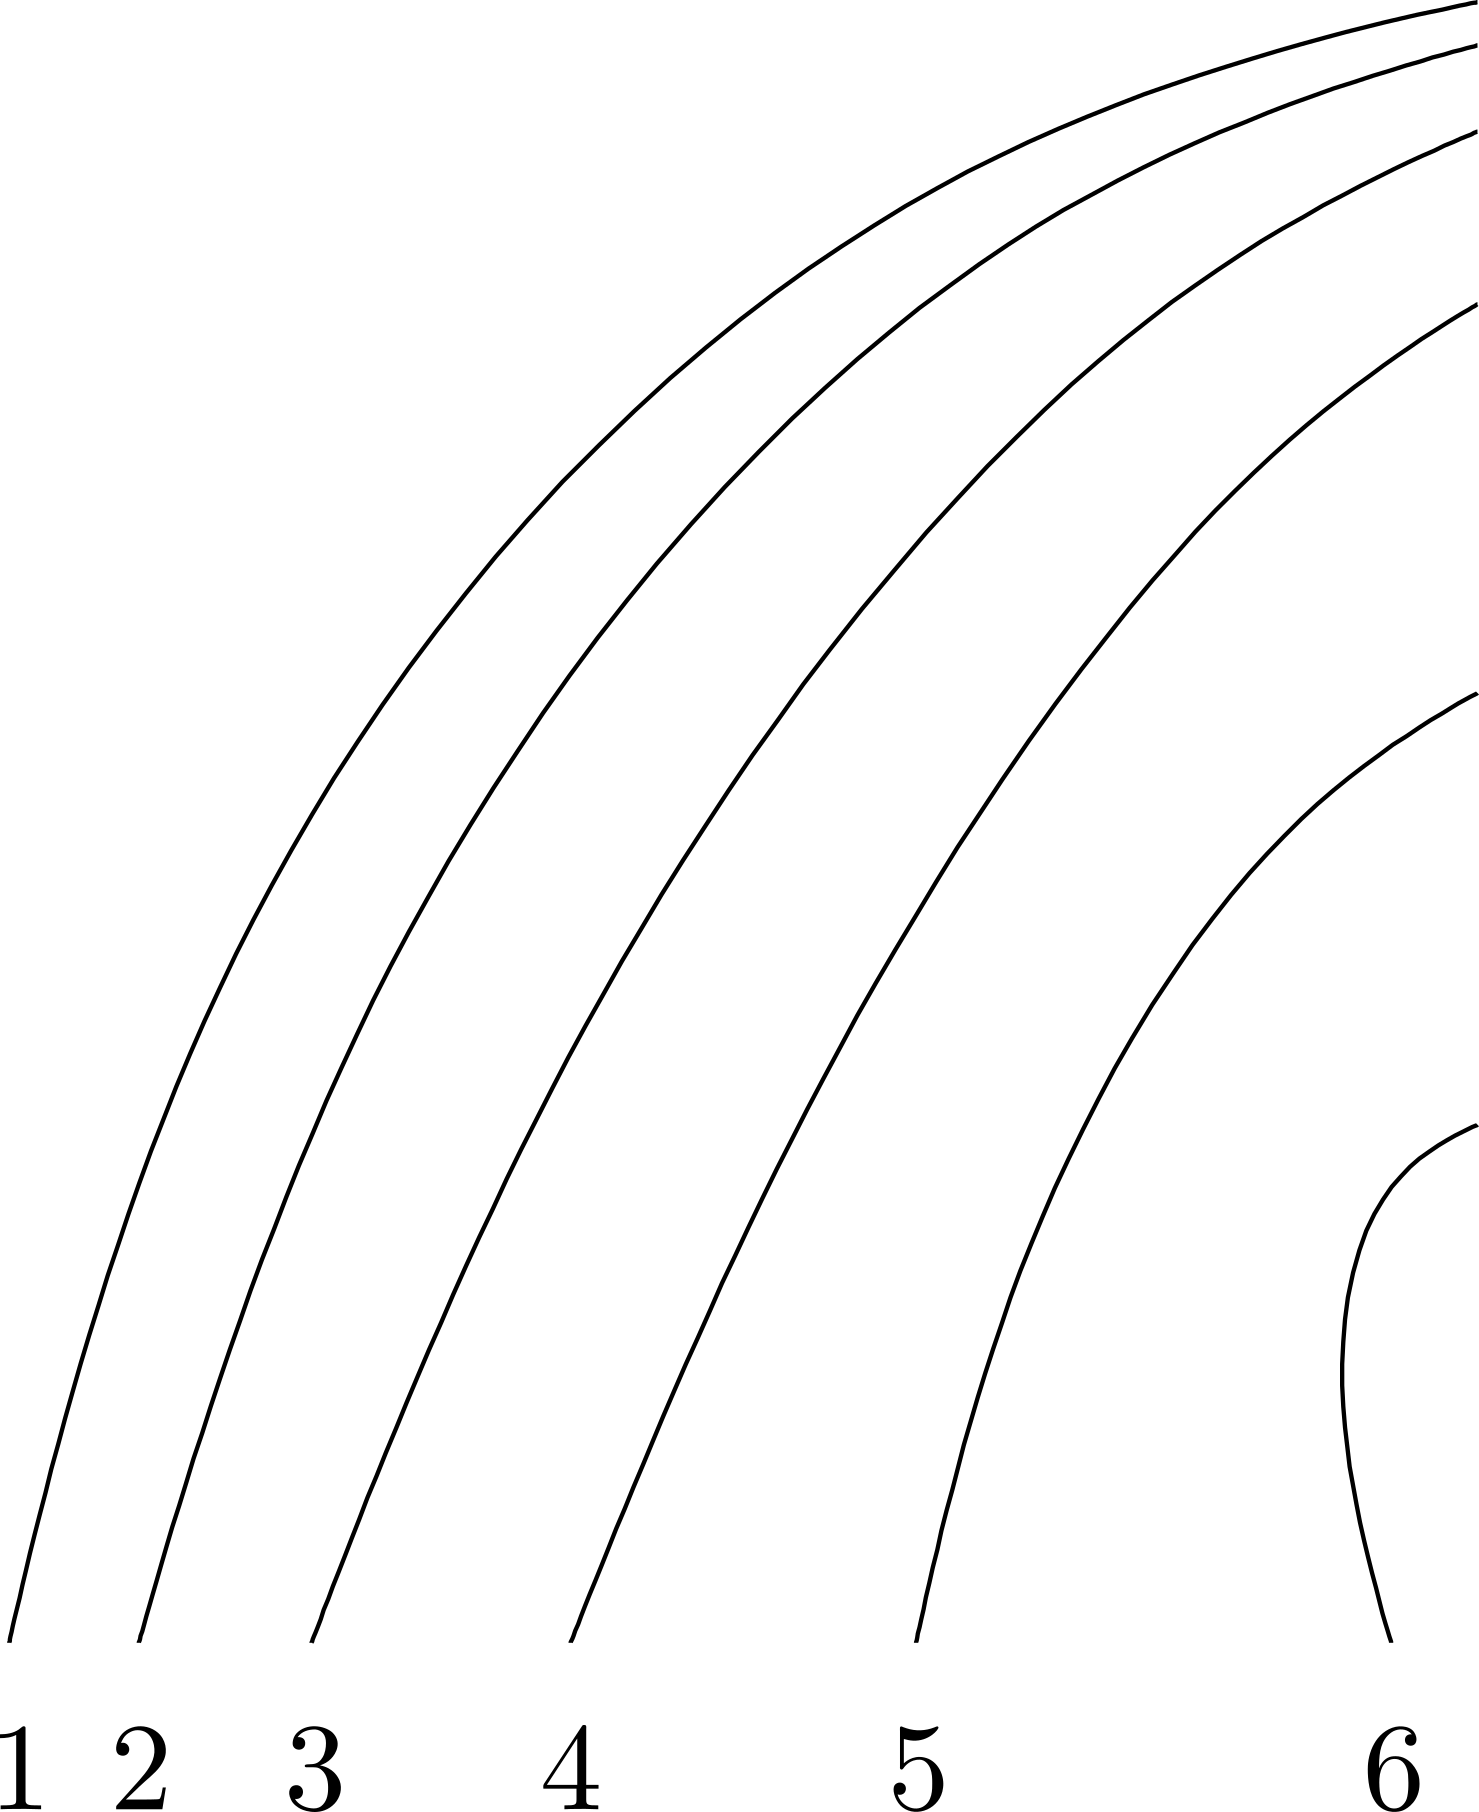
\includegraphics[width=.5\textwidth]{../Graphics/113b.png}\hfil

%%% Local Variables:
%%% mode: latex
%%% TeX-master: "../LectureNotes-Optimization"
%%% End:



\chapter{Convex optimization problems}

\clearpage
\section{Optimization problems}

\clearpage
\section{Convex optimization}

\clearpage
\section{Linear optimization problems}

\clearpage
\section{Quadratic optimization problems}

\clearpage
\section{Geometric programming}

\clearpage
\section{Generalized inequality constraints}

\clearpage
\section{Vector optimization}


\clearpage
\hfil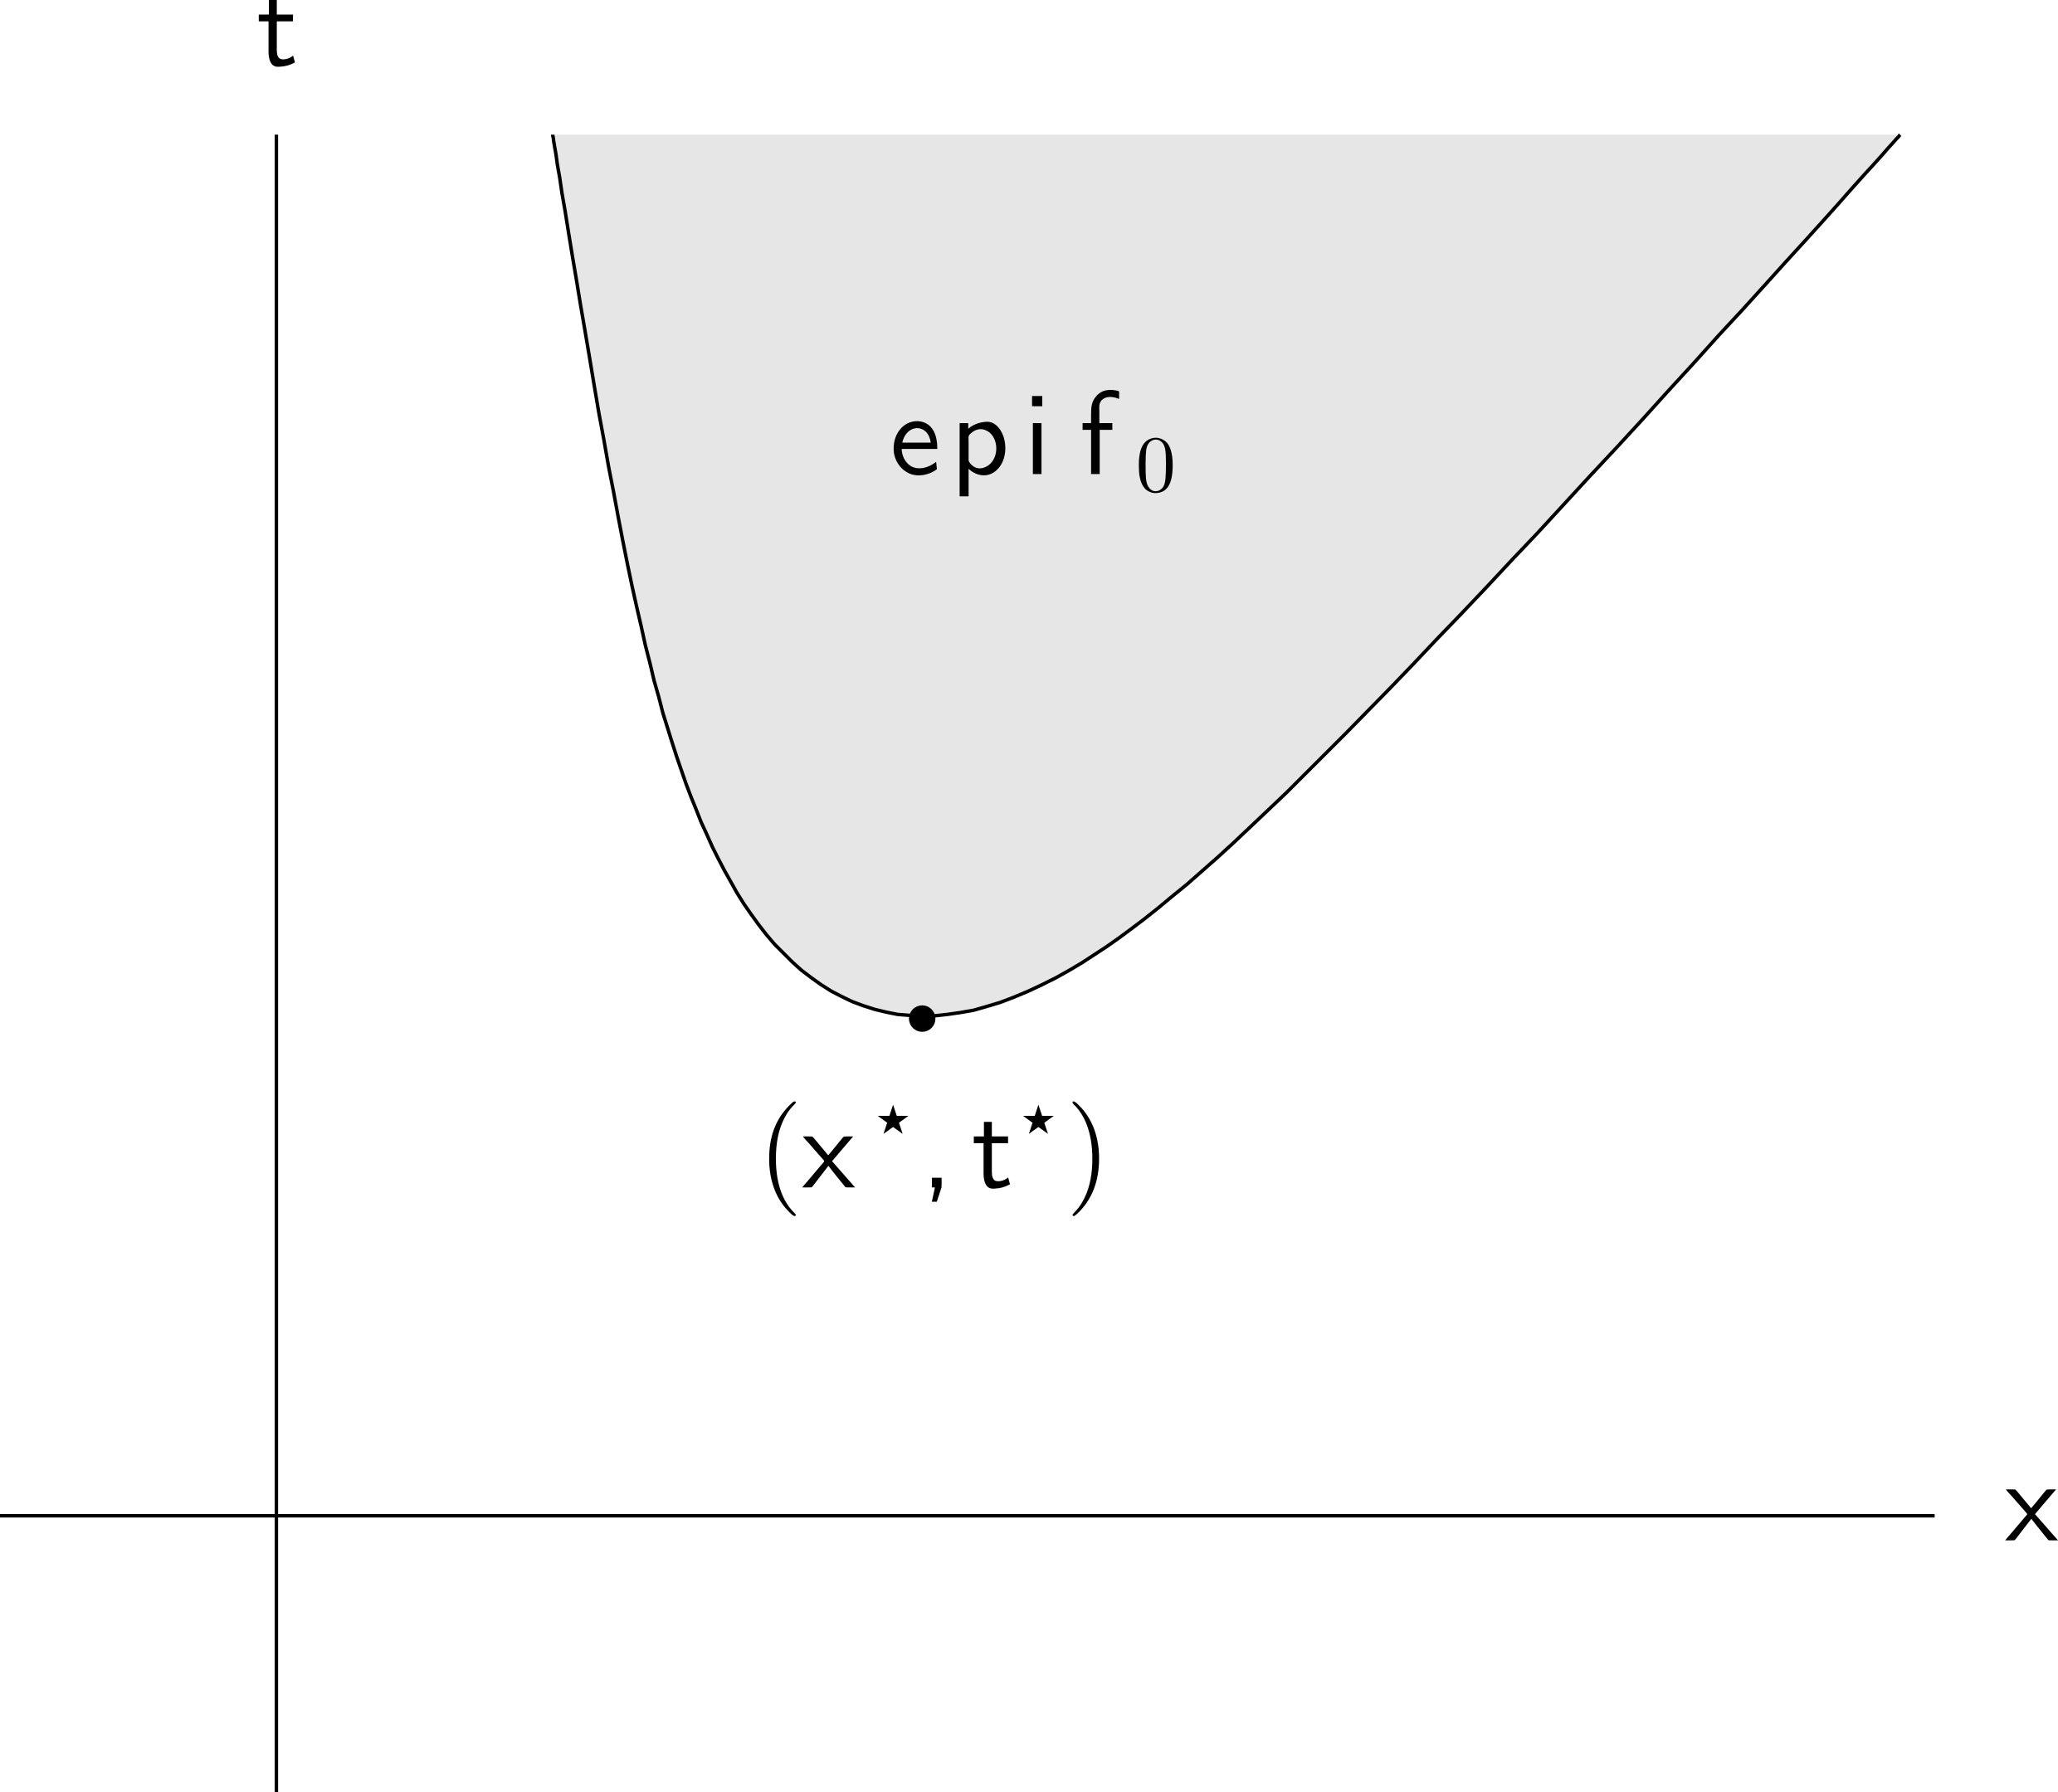
\includegraphics[width=.5\textwidth]{../Graphics/135.png}\hfil

\clearpage
\hfil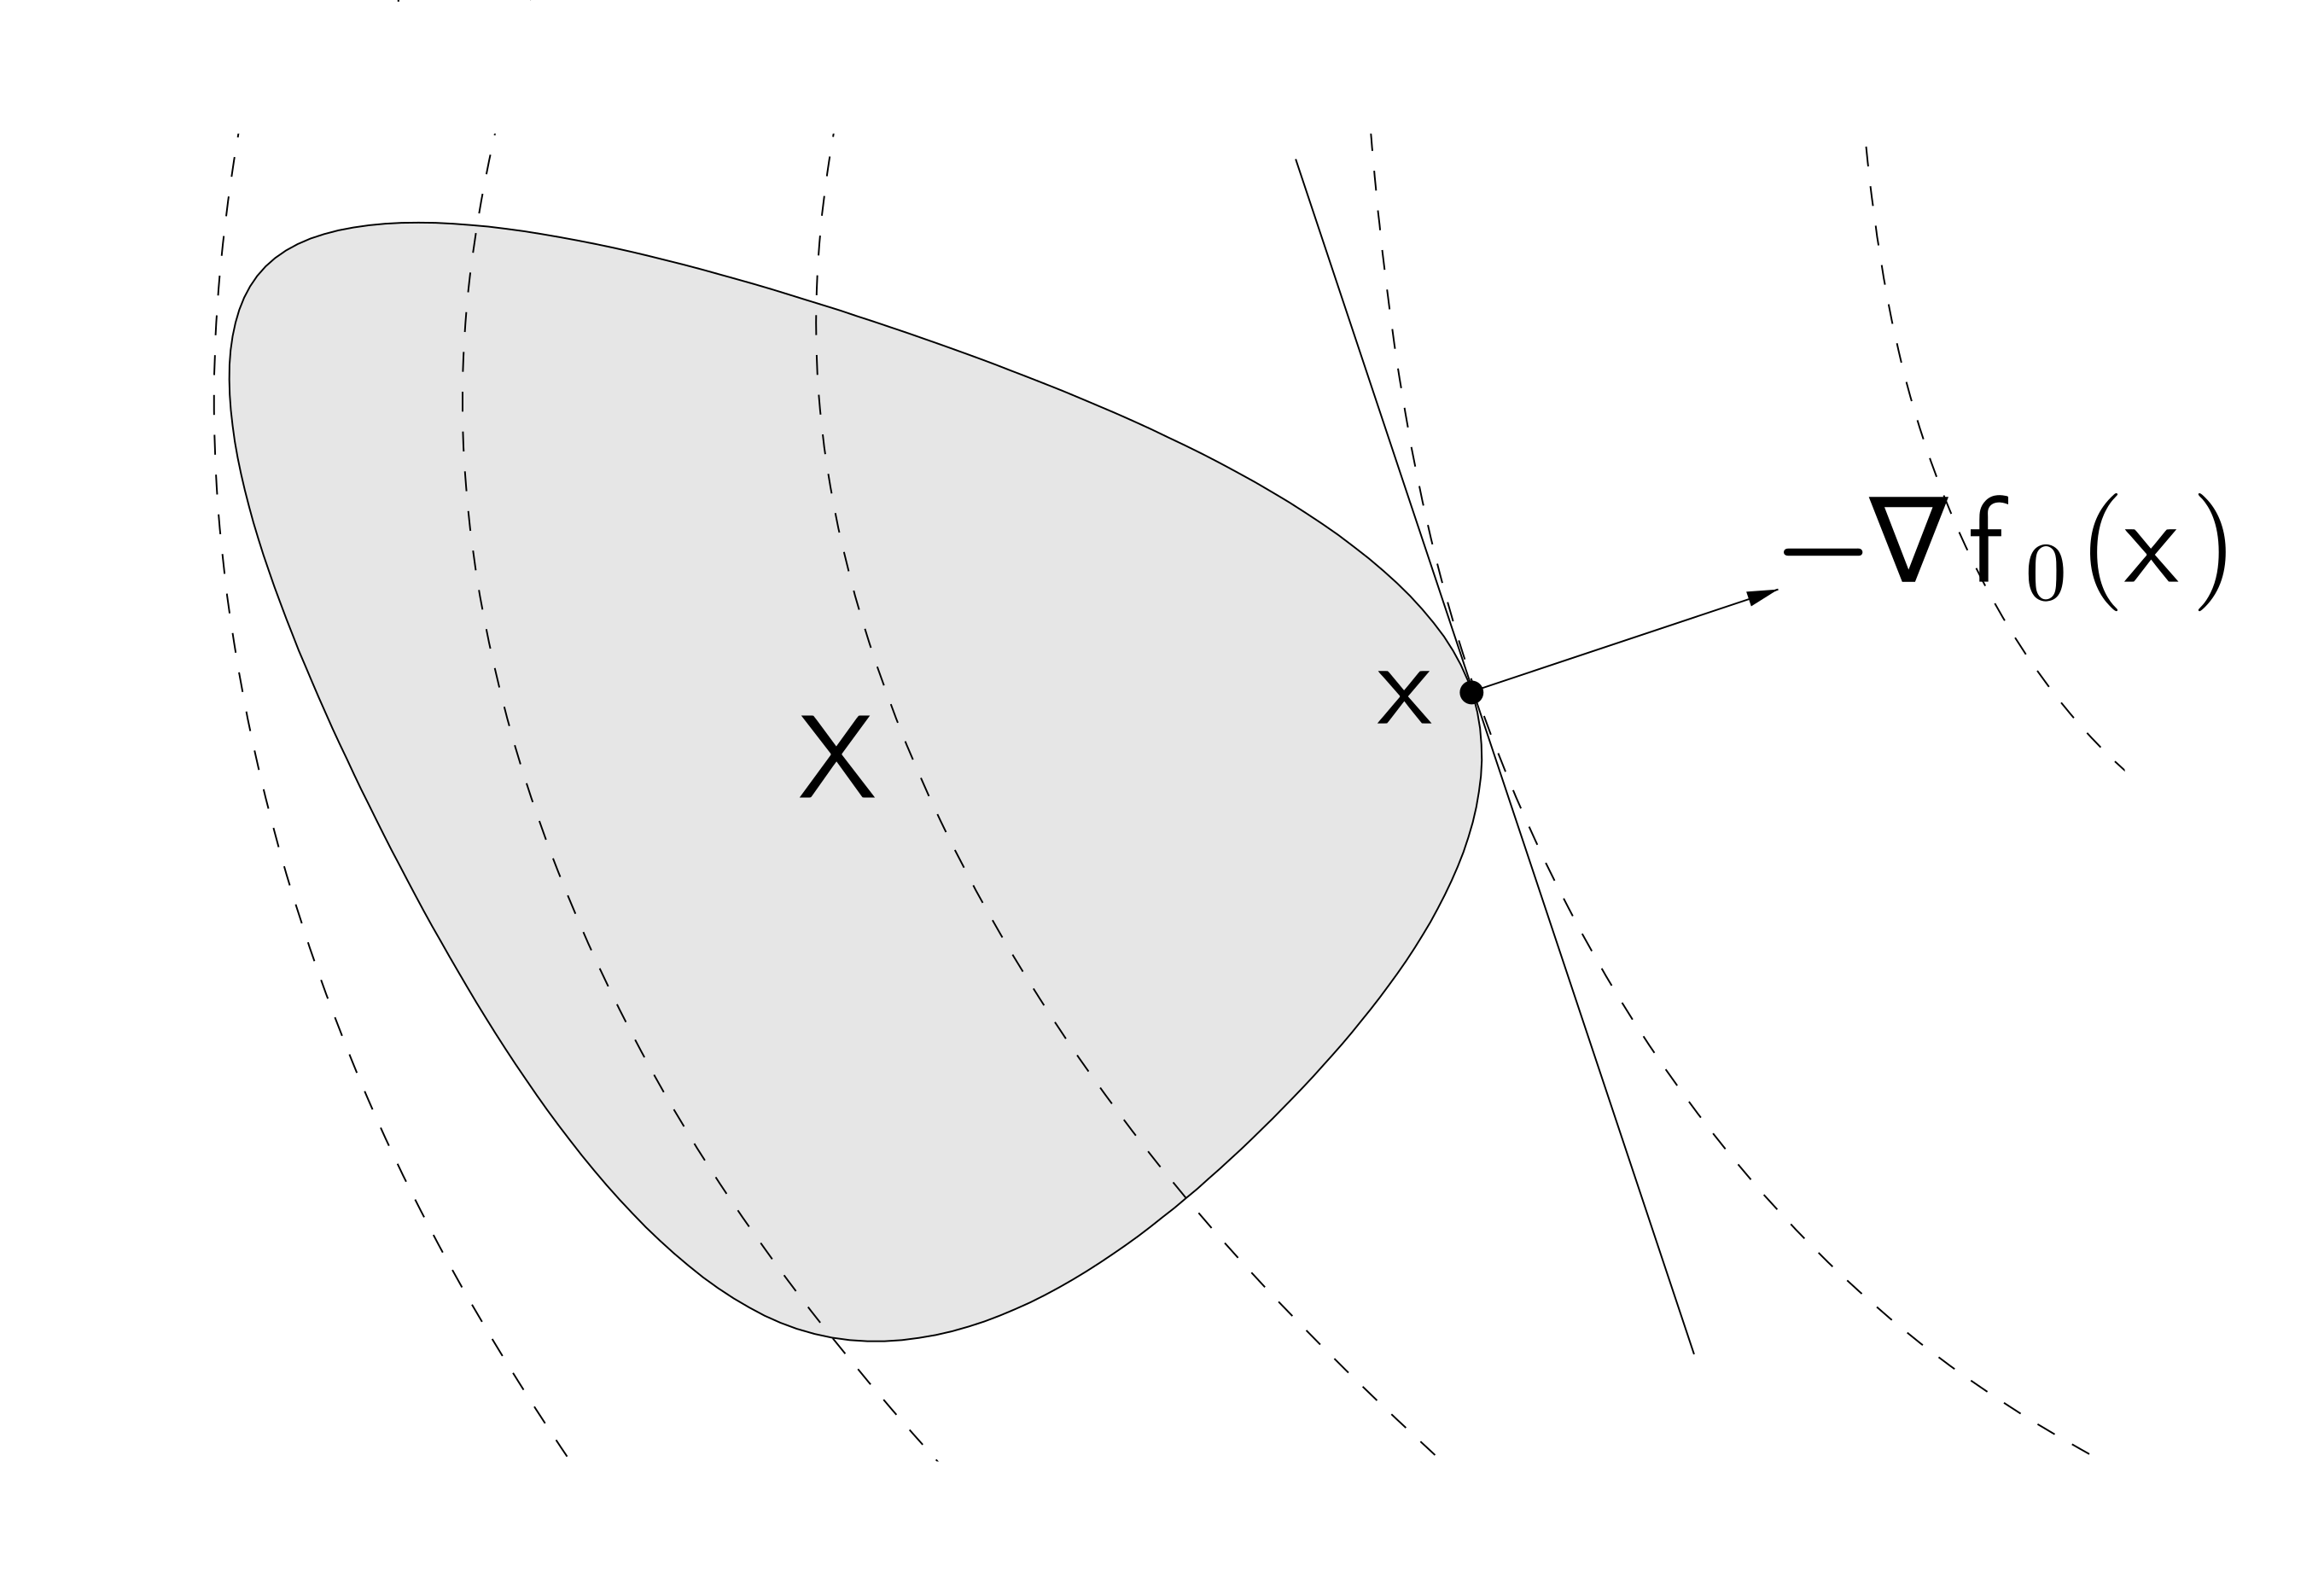
\includegraphics[width=.5\textwidth]{../Graphics/139.png}\hfil

\clearpage
\hfil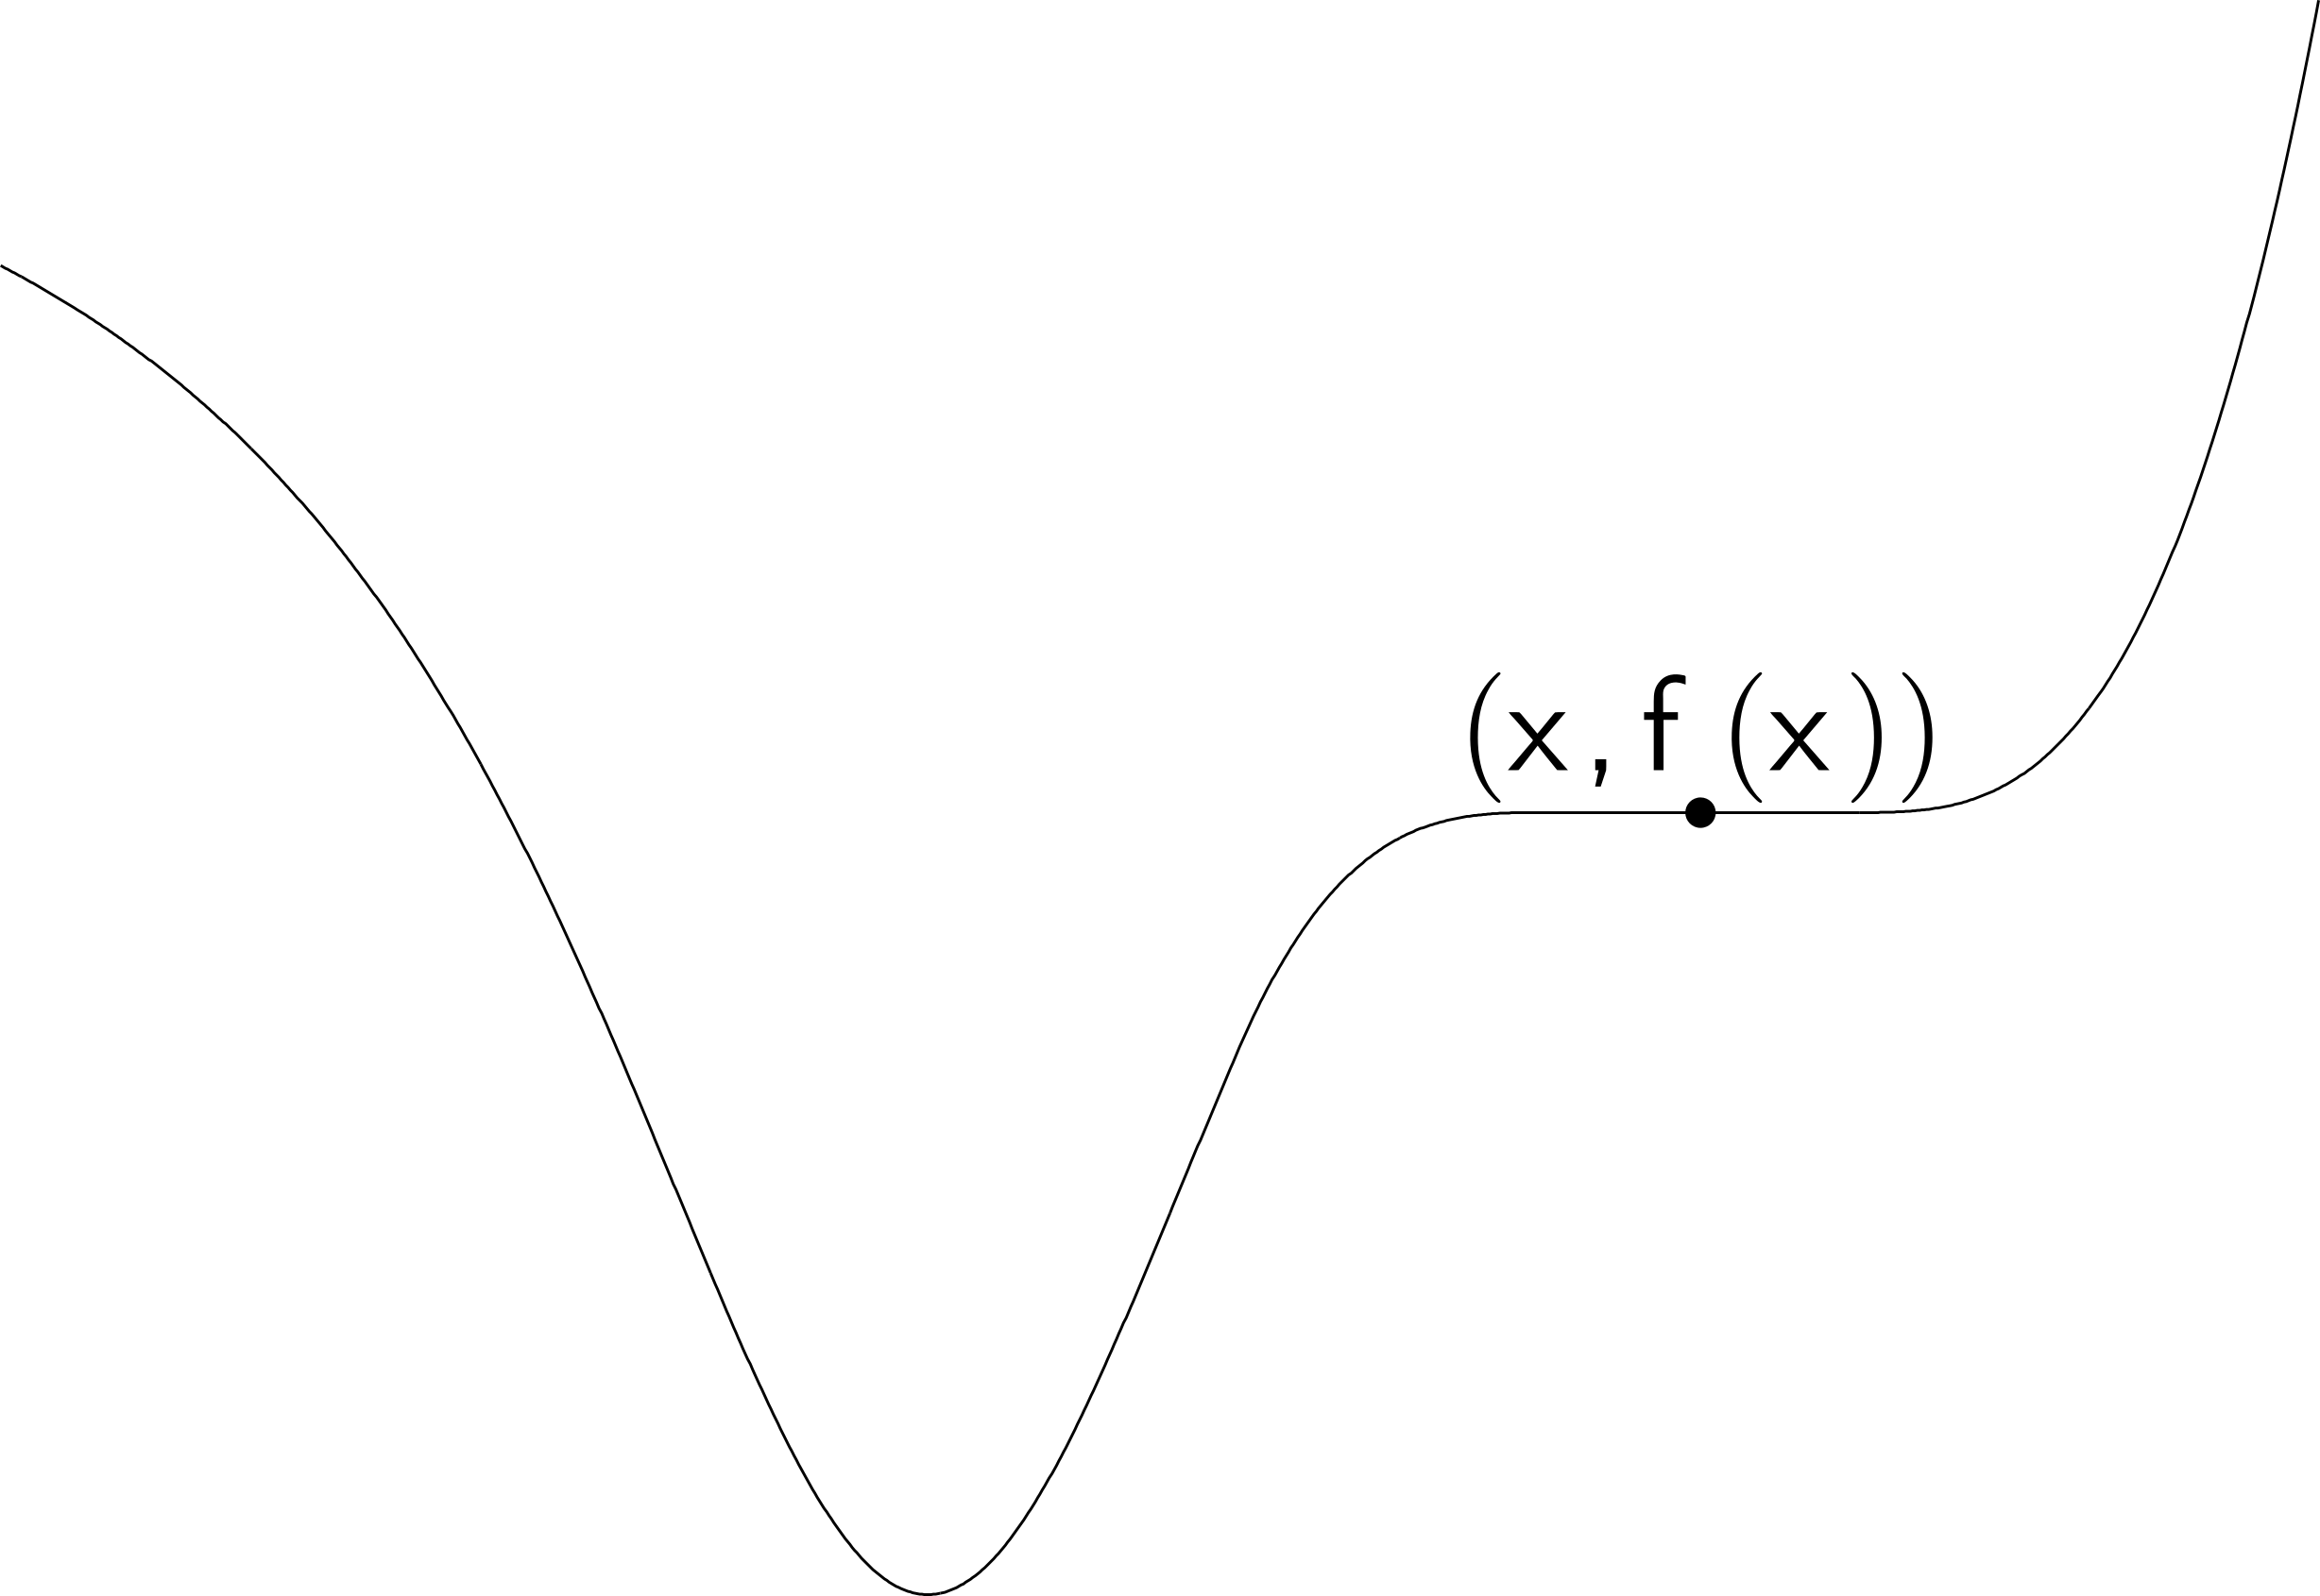
\includegraphics[width=.5\textwidth]{../Graphics/145.png}\hfil

\clearpage
\hfil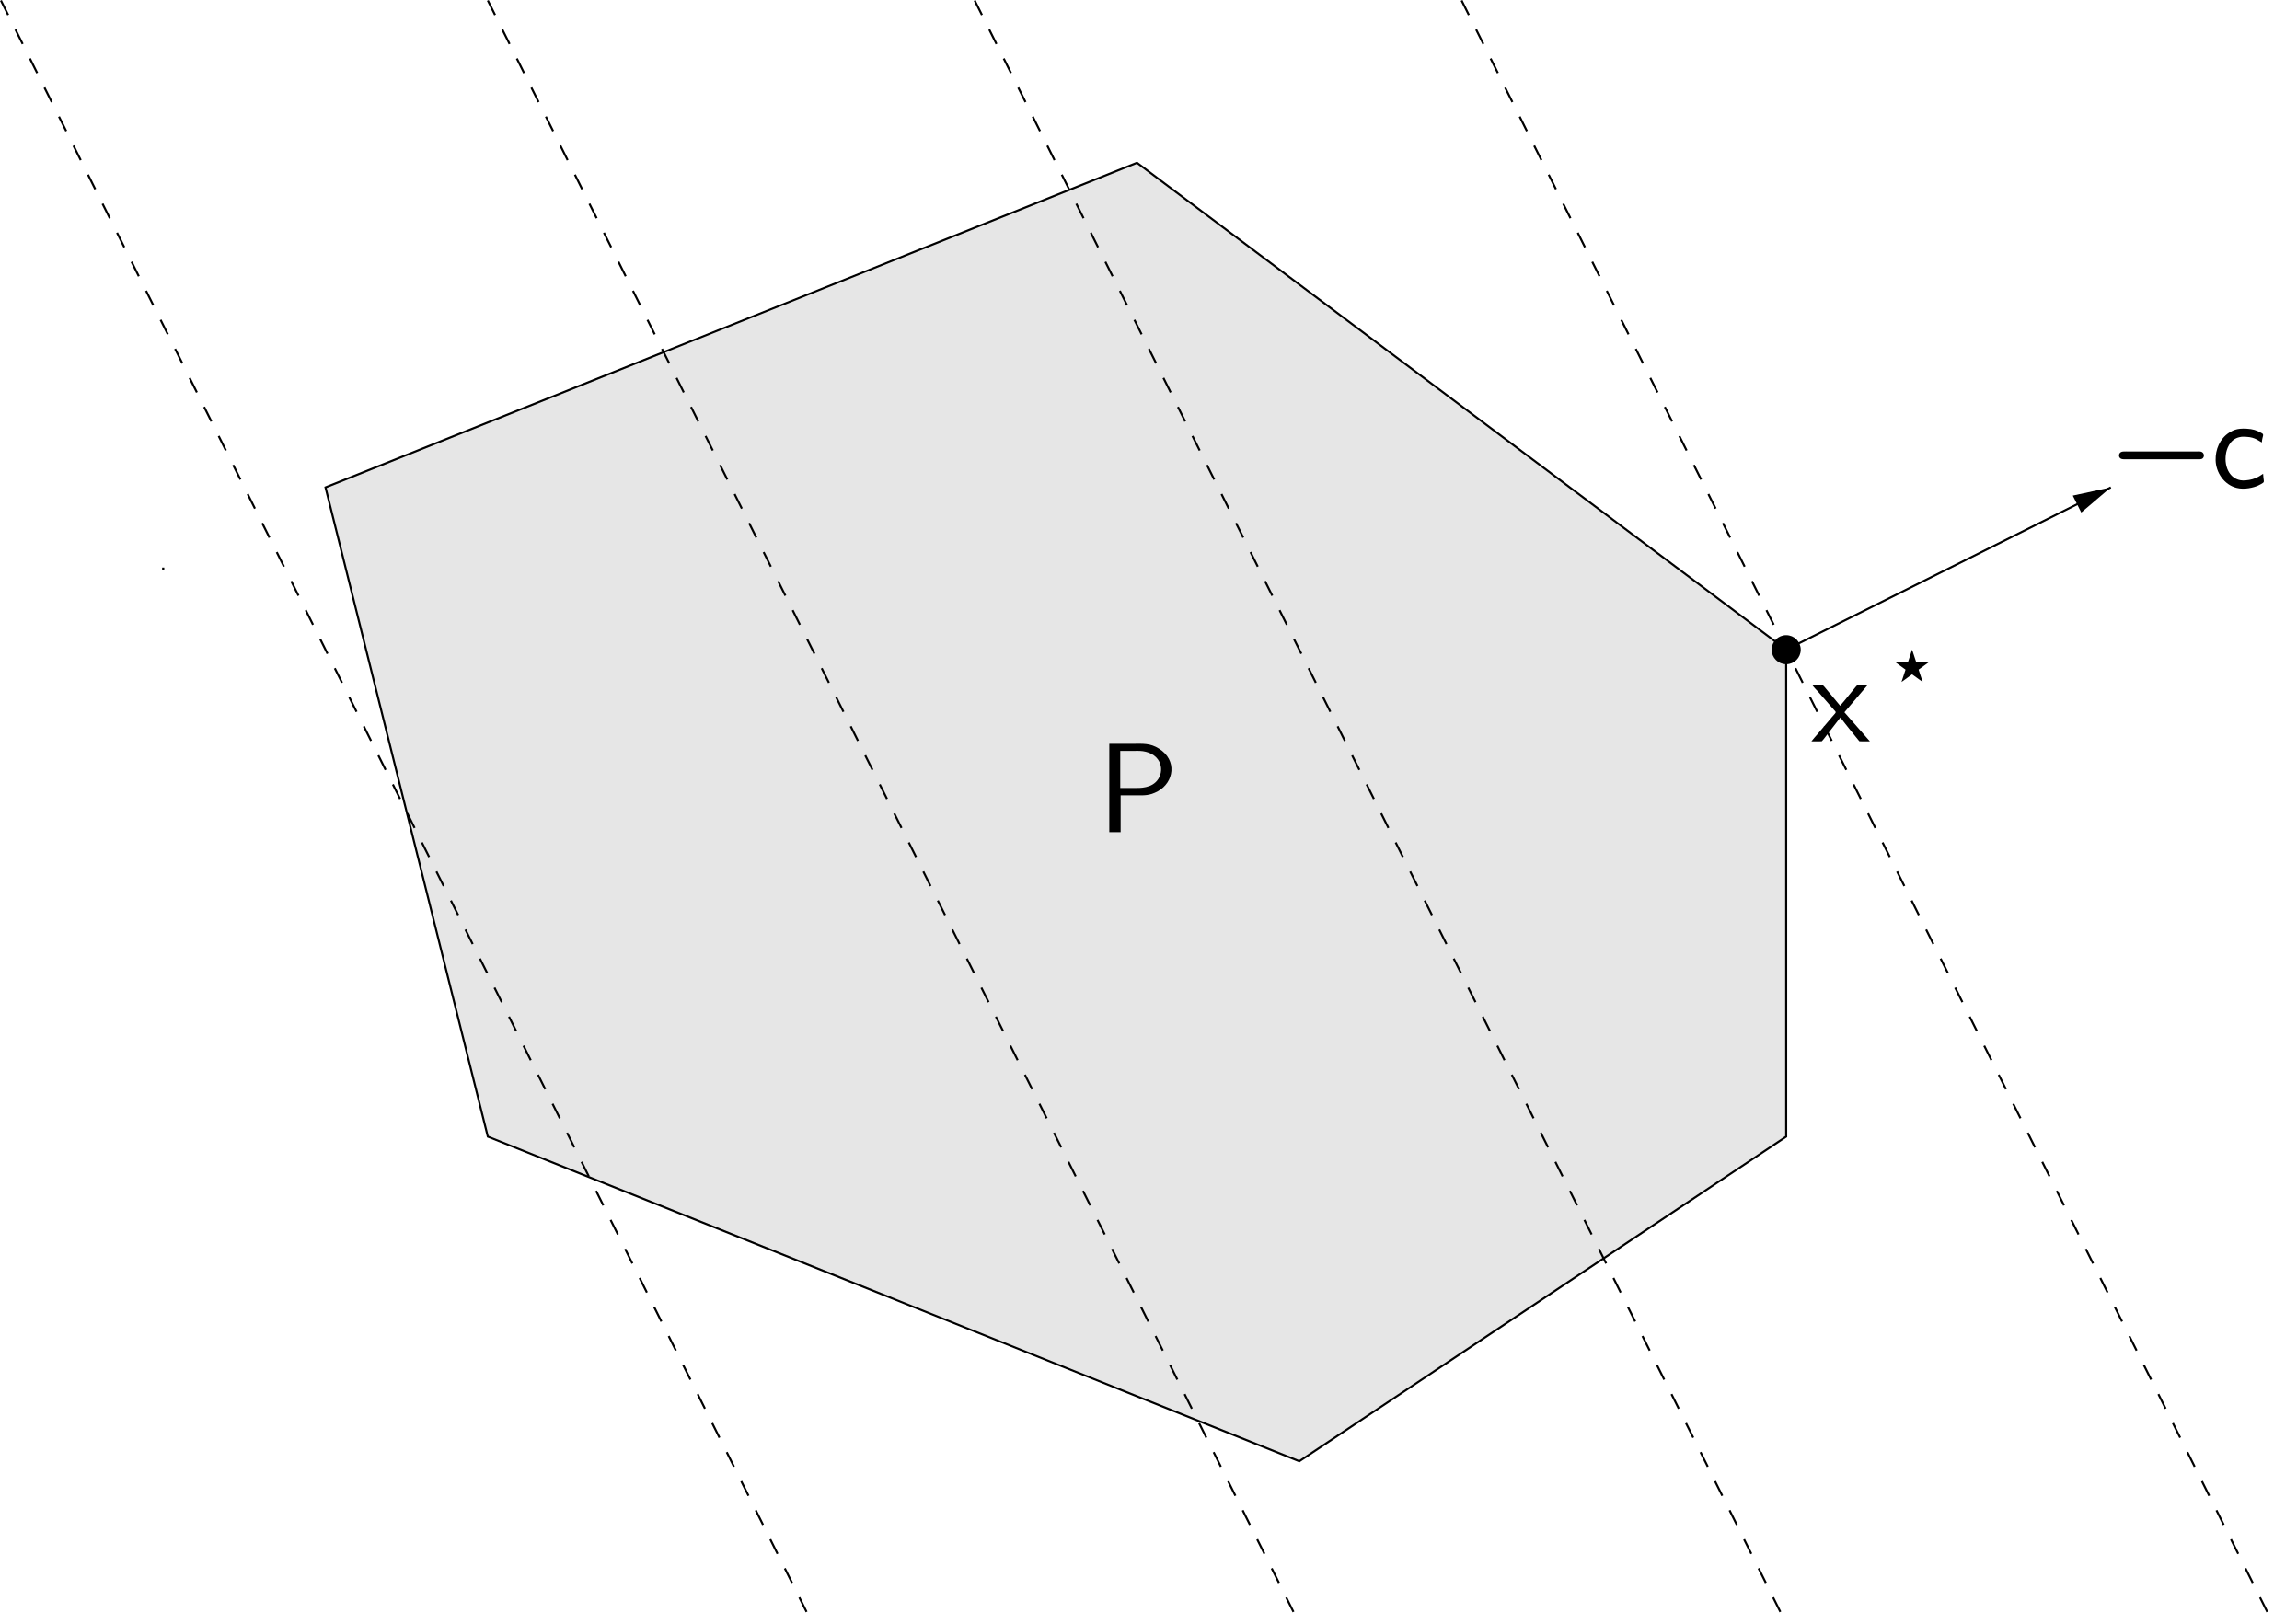
\includegraphics[width=.5\textwidth]{../Graphics/147.png}\hfil

\clearpage
\hfil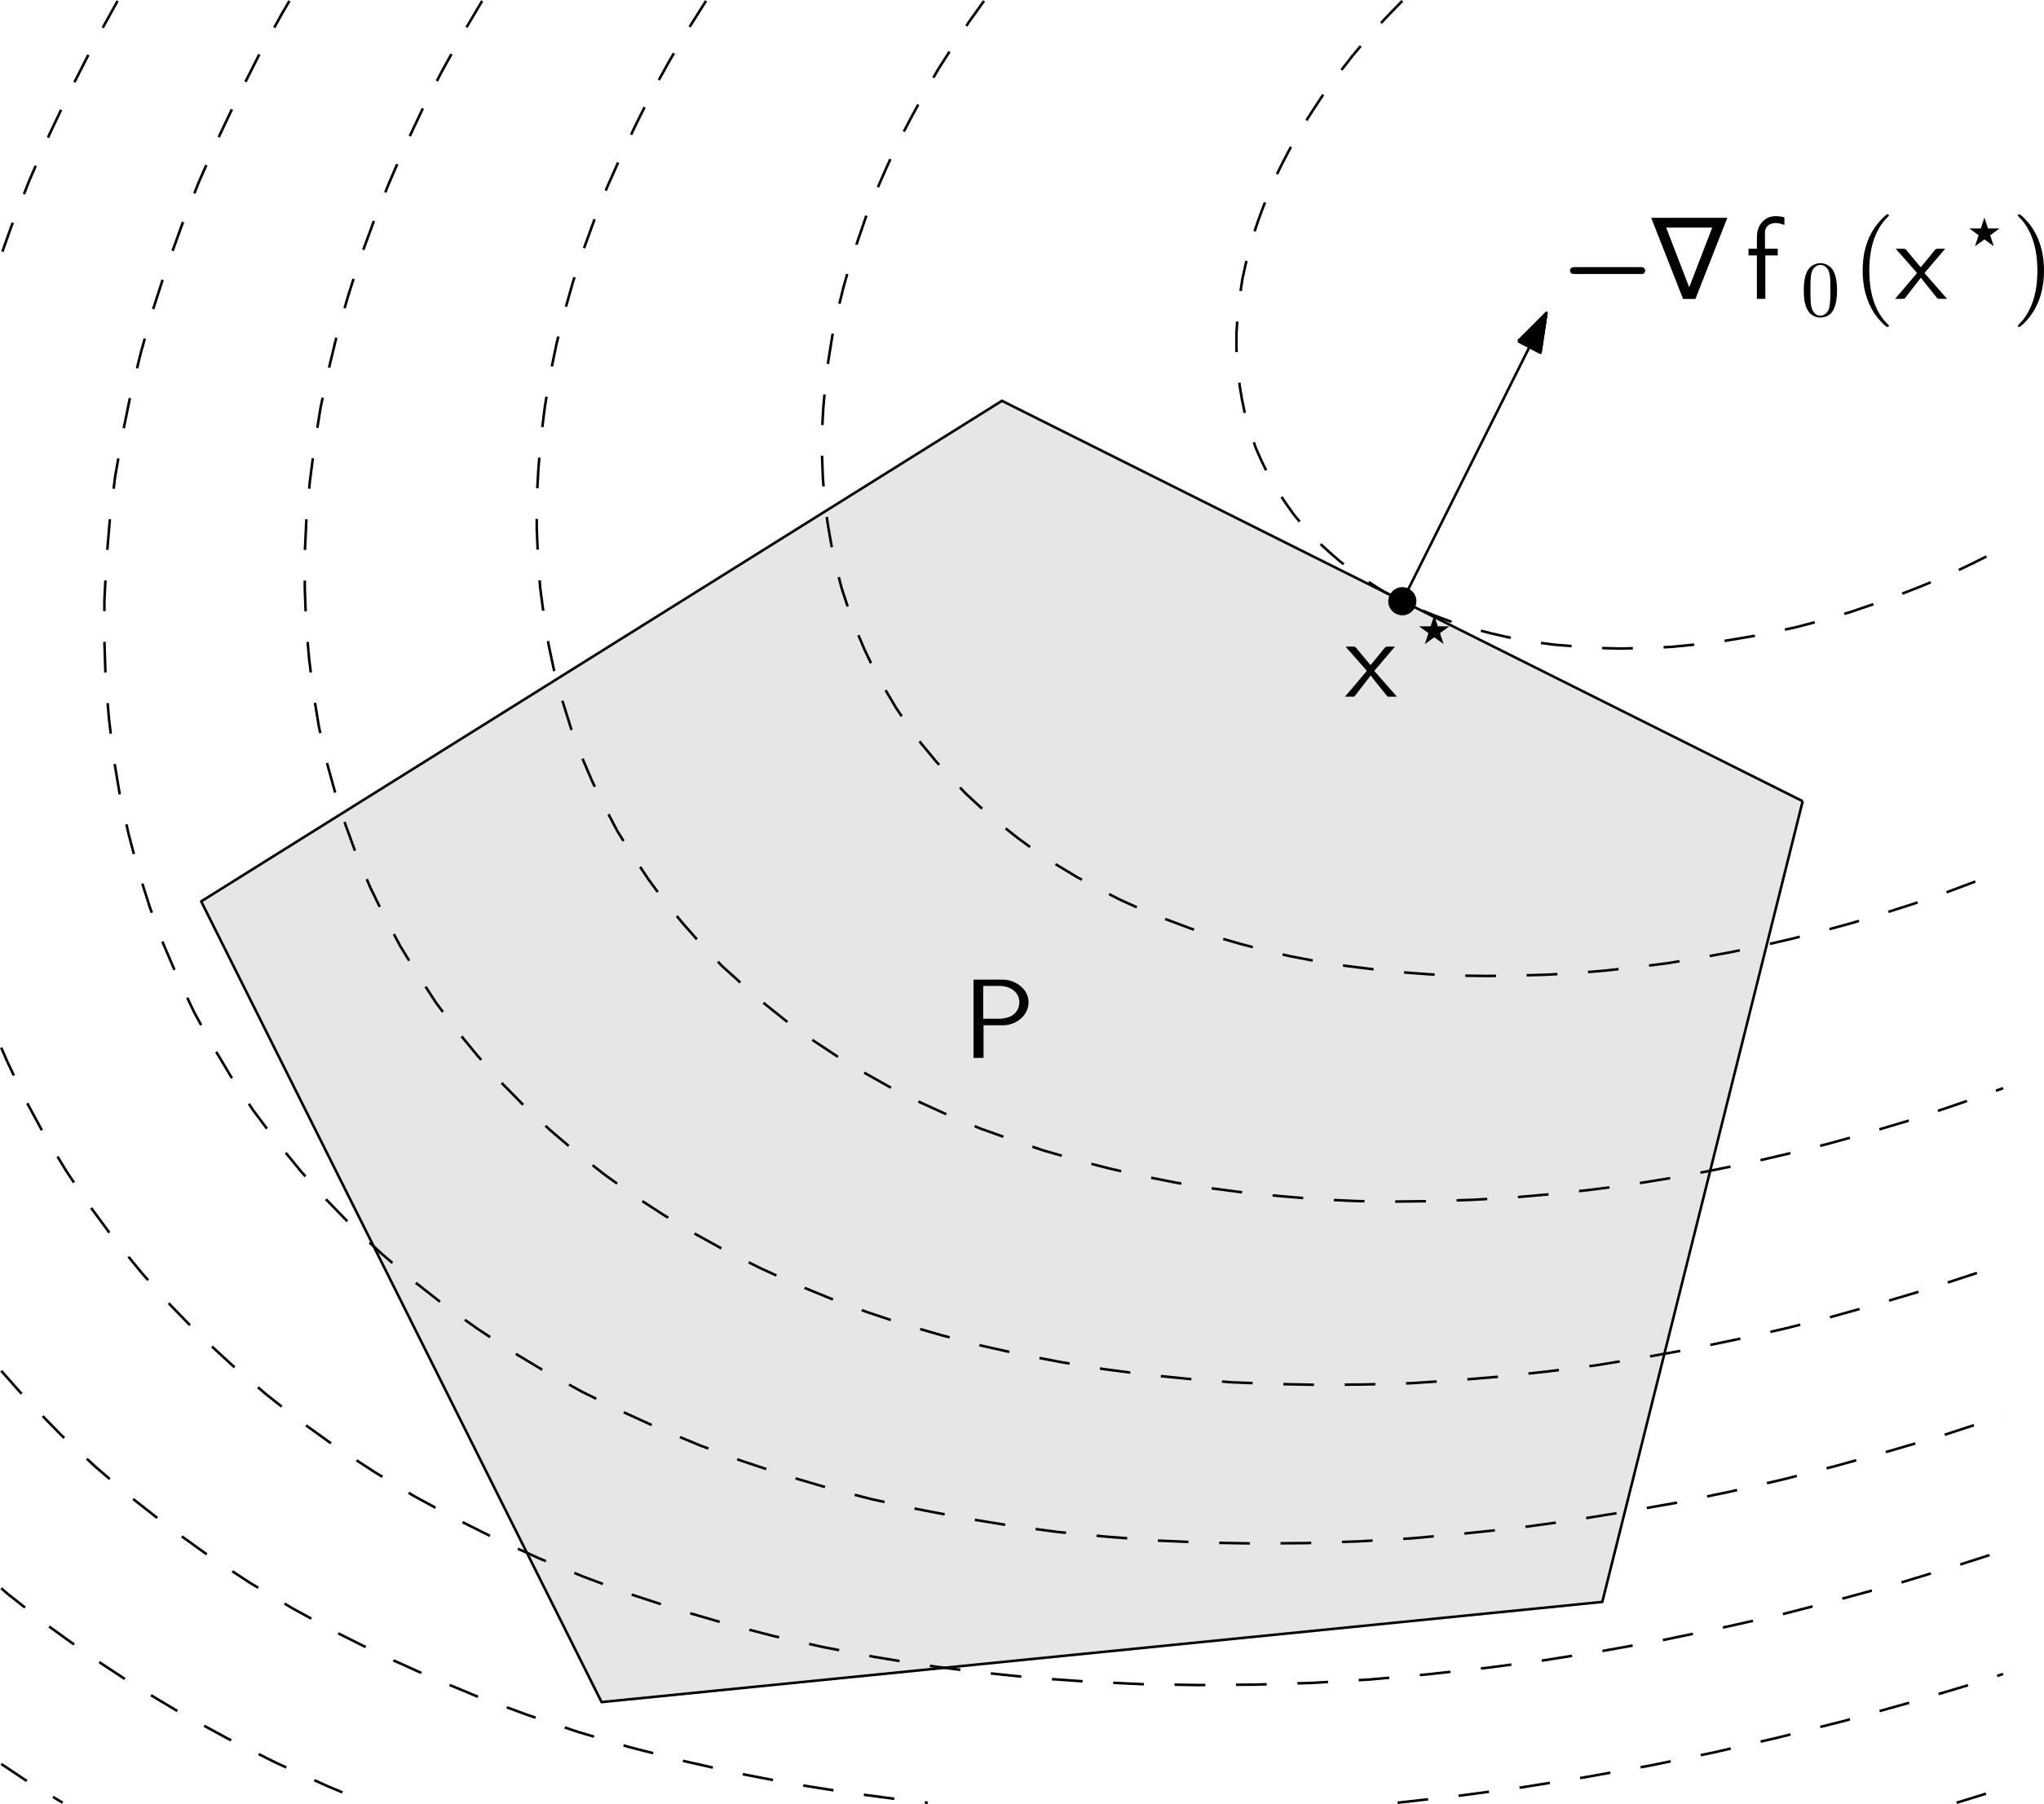
\includegraphics[width=.5\textwidth]{../Graphics/153.png}\hfil

\clearpage
\hfil\includegraphics[width=.5\textwidth]{../Graphics/164.png}\hfil

\clearpage
\hfil\includegraphics[width=.5\textwidth]{../Graphics/176.png}\hfil

\clearpage
\hfil\includegraphics[width=.5\textwidth]{../Graphics/178.png}\hfil

\clearpage
\hfil\includegraphics[width=.5\textwidth]{../Graphics/179.png}\hfil

\clearpage
\hfil\includegraphics[width=.5\textwidth]{../Graphics/181.png}\hfil

\clearpage
\hfil\includegraphics[width=.5\textwidth]{../Graphics/185.png}\hfil

\clearpage
\hfil\includegraphics[width=.5\textwidth]{../Graphics/187.png}\hfil

\clearpage
\hfil\includegraphics[width=.5\textwidth]{../Graphics/212.png}\hfil

%%% Local Variables:
%%% mode: latex
%%% TeX-master: "../LectureNotes-Optimization"
%%% End:



\chapter{Duality}

\clearpage
\section{The Lagrange dual function}

\clearpage
\section{The Lagrange dual problem}

\clearpage
\section{Geometric interpretation}

\clearpage
\section{Saddle-point interpretation}

\clearpage
\section{Optimality conditions}

\clearpage
\section{Perturbation and sensitivity analysis}

\clearpage
\section{Examples}

\clearpage
\section{Theorems of alternatives}

\clearpage
\section{Generalized inequalities}


\clearpage
\hfil\includegraphics[width=.5\textwidth]{../Graphics/217a.png}\hfil

\clearpage
\hfil\includegraphics[width=.5\textwidth]{../Graphics/217b.png}\hfil

\clearpage
\hfil\includegraphics[width=.5\textwidth]{../Graphics/233a.png}\hfil

\clearpage
\hfil\includegraphics[width=.5\textwidth]{../Graphics/233b.png}\hfil

\clearpage
\hfil\includegraphics[width=.5\textwidth]{../Graphics/234.png}\hfil

\clearpage
\hfil\includegraphics[width=.5\textwidth]{../Graphics/236.png}\hfil

\clearpage
\hfil\includegraphics[width=.5\textwidth]{../Graphics/246a.png}\hfil

\clearpage
\hfil\includegraphics[width=.5\textwidth]{../Graphics/246b.png}\hfil

\clearpage
\hfil\includegraphics[width=.5\textwidth]{../Graphics/247.png}\hfil

\clearpage
\hfil\includegraphics[width=.5\textwidth]{../Graphics/251.png}\hfil

%%% Local Variables:
%%% mode: latex
%%% TeX-master: "../LectureNotes-Optimization"
%%% End:



\chapter{Approximation and fitting}

\clearpage
\section{Norm approximation}

\clearpage
\section{Least-norm problems}

\clearpage
\section{Regularized approximation}

\clearpage
\section{Robust approximation}

\clearpage
\section{Function fitting and interpolation}


\clearpage
\hfil\includegraphics[width=.5\textwidth]{../Graphics/295.png}\hfil

\clearpage
\hfil\includegraphics[width=.5\textwidth]{../Graphics/297.png}\hfil

\clearpage
\hfil\includegraphics[width=.5\textwidth]{../Graphics/298.png}\hfil

\clearpage
\hfil\includegraphics[width=.5\textwidth]{../Graphics/299.png}\hfil

\clearpage
\hfil\includegraphics[width=.5\textwidth]{../Graphics/300.png}\hfil

\clearpage
\hfil\includegraphics[width=.5\textwidth]{../Graphics/309.png}\hfil

\clearpage
\hfil\includegraphics[width=.5\textwidth]{../Graphics/311.png}\hfil

\clearpage
\hfil\includegraphics[width=.5\textwidth]{../Graphics/313a.png}\hfil

\clearpage
\hfil\includegraphics[width=.5\textwidth]{../Graphics/313b.png}\hfil

\clearpage
\hfil\includegraphics[width=.5\textwidth]{../Graphics/314.png}\hfil

\clearpage
\hfil\includegraphics[width=.5\textwidth]{../Graphics/315.png}\hfil

\clearpage
\hfil\includegraphics[width=.5\textwidth]{../Graphics/316a.png}\hfil

\clearpage
\hfil\includegraphics[width=.5\textwidth]{../Graphics/316b.png}\hfil

\clearpage
\hfil\includegraphics[width=.5\textwidth]{../Graphics/317.png}\hfil

\clearpage
\hfil\includegraphics[width=.5\textwidth]{../Graphics/320.png}\hfil

\clearpage
\hfil\includegraphics[width=.5\textwidth]{../Graphics/325.png}\hfil

\clearpage
\hfil\includegraphics[width=.5\textwidth]{../Graphics/327.png}\hfil

\clearpage
\hfil\includegraphics[width=.5\textwidth]{../Graphics/328.png}\hfil

\clearpage
\hfil\includegraphics[width=.5\textwidth]{../Graphics/332a.png}\hfil

\clearpage
\hfil\includegraphics[width=.5\textwidth]{../Graphics/332b.png}\hfil

\clearpage
\hfil\includegraphics[width=.5\textwidth]{../Graphics/335.png}\hfil

\clearpage
\hfil\includegraphics[width=.5\textwidth]{../Graphics/336.png}\hfil

\clearpage
\hfil\includegraphics[width=.5\textwidth]{../Graphics/337.png}\hfil

\clearpage
\hfil\includegraphics[width=.5\textwidth]{../Graphics/339.png}\hfil

\clearpage
\hfil\includegraphics[width=.5\textwidth]{../Graphics/342a.png}\hfil

\clearpage
\hfil\includegraphics[width=.5\textwidth]{../Graphics/342b.png}\hfil

%%% Local Variables:
%%% mode: latex
%%% TeX-master: "../LectureNotes-Optimization"
%%% End:



\chapter{Statistical estimation}

\clearpage
\section{Parametric distribution estimation}

\clearpage
\section{Nonparametric distribution estimation}

\clearpage
\section{Optimal detector design and hypothesis testing}

\clearpage
\section{Chebyshev and Chernoff bounds}

\clearpage
\section{Experiment design}


\clearpage
\hfil\includegraphics[width=.5\textwidth]{../Graphics/355.png}\hfil

\clearpage
\hfil\includegraphics[width=.5\textwidth]{../Graphics/363.png}\hfil

\clearpage
\hfil\includegraphics[width=.5\textwidth]{../Graphics/364.png}\hfil

\clearpage
\hfil\includegraphics[width=.5\textwidth]{../Graphics/371.png}\hfil

\clearpage
\hfil\includegraphics[width=.5\textwidth]{../Graphics/382.png}\hfil

\clearpage
\hfil\includegraphics[width=.5\textwidth]{../Graphics/383a.png}\hfil

\clearpage
\hfil\includegraphics[width=.5\textwidth]{../Graphics/383b.png}\hfil

\clearpage
\hfil\includegraphics[width=.5\textwidth]{../Graphics/384.png}\hfil

\clearpage
\hfil\includegraphics[width=.5\textwidth]{../Graphics/389a.png}\hfil

\clearpage
\hfil\includegraphics[width=.5\textwidth]{../Graphics/389b.png}\hfil

\clearpage
\hfil\includegraphics[width=.5\textwidth]{../Graphics/389c.png}\hfil

\clearpage
\hfil\includegraphics[width=.5\textwidth]{../Graphics/390.png}\hfil

%%% Local Variables:
%%% mode: latex
%%% TeX-master: "../LectureNotes-Optimization"
%%% End:



\chapter{Geometric problems}

\clearpage
\section{Projection on a set}

\clearpage
\section{Distance between sets}

\clearpage
\section{Euclidean distance and angle problems}

\clearpage
\section{Extremal volume ellipsoids}

\clearpage
\section{Centering}

\clearpage
\section{Classification}

\clearpage
\section{Placement and location}

\clearpage
\section{Floor planning}


\clearpage
\hfil\includegraphics[width=.5\textwidth]{../Graphics/400.png}\hfil

\clearpage
\hfil\includegraphics[width=.5\textwidth]{../Graphics/403.png}\hfil

\clearpage
\hfil\includegraphics[width=.5\textwidth]{../Graphics/412.png}\hfil

\clearpage
\hfil\includegraphics[width=.5\textwidth]{../Graphics/416.png}\hfil

\clearpage
\hfil\includegraphics[width=.5\textwidth]{../Graphics/417.png}\hfil

\clearpage
\hfil\includegraphics[width=.5\textwidth]{../Graphics/419.png}\hfil

\clearpage
\hfil\includegraphics[width=.5\textwidth]{../Graphics/421.png}\hfil

\clearpage
\hfil\includegraphics[width=.5\textwidth]{../Graphics/423.png}\hfil

\clearpage
\hfil\includegraphics[width=.5\textwidth]{../Graphics/425.png}\hfil

\clearpage
\hfil\includegraphics[width=.5\textwidth]{../Graphics/426.png}\hfil

\clearpage
\hfil\includegraphics[width=.5\textwidth]{../Graphics/427.png}\hfil

\clearpage
\hfil\includegraphics[width=.5\textwidth]{../Graphics/429.png}\hfil

\clearpage
\hfil\includegraphics[width=.5\textwidth]{../Graphics/431a.png}\hfil

\clearpage
\hfil\includegraphics[width=.5\textwidth]{../Graphics/431b.png}\hfil

\clearpage
\hfil\includegraphics[width=.5\textwidth]{../Graphics/435a.png}\hfil

\clearpage
\hfil\includegraphics[width=.5\textwidth]{../Graphics/435b.png}\hfil

\clearpage
\hfil\includegraphics[width=.5\textwidth]{../Graphics/436.png}\hfil

\clearpage
\hfil\includegraphics[width=.5\textwidth]{../Graphics/439.png}\hfil

\clearpage
\hfil\includegraphics[width=.5\textwidth]{../Graphics/441.png}\hfil

\clearpage
\hfil\includegraphics[width=.5\textwidth]{../Graphics/444.png}\hfil

\clearpage
\hfil\includegraphics[width=.5\textwidth]{../Graphics/453a.png}\hfil

\clearpage
\hfil\includegraphics[width=.5\textwidth]{../Graphics/453b.png}\hfil

%%% Local Variables:
%%% mode: latex
%%% TeX-master: "../LectureNotes-Optimization"
%%% End:



\chapter{Unconstrained minimization}

\clearpage
\section{Unconstrained minimization}

\clearpage
\section{Descent methods}

\clearpage
\section{Gradient descent method}

\clearpage
\section{Steepest descent method}

\clearpage
\section{Newton’s method}

\clearpage
\section{Self-concordance}

\clearpage
\section{Implementation}


\clearpage
\hfil\includegraphics[width=.5\textwidth]{../Graphics/465.png}\hfil

\clearpage
\hfil\includegraphics[width=.5\textwidth]{../Graphics/469.png}\hfil

\clearpage
\hfil\includegraphics[width=.5\textwidth]{../Graphics/471a.png}\hfil

\clearpage
\hfil\includegraphics[width=.5\textwidth]{../Graphics/471b.png}\hfil

\clearpage
\hfil\includegraphics[width=.5\textwidth]{../Graphics/472.png}\hfil

\clearpage
\hfil\includegraphics[width=.5\textwidth]{../Graphics/473.png}\hfil

\clearpage
\hfil\includegraphics[width=.5\textwidth]{../Graphics/474a.png}\hfil

\clearpage
\hfil\includegraphics[width=.5\textwidth]{../Graphics/474b.png}\hfil

\clearpage
\hfil\includegraphics[width=.5\textwidth]{../Graphics/477.png}\hfil

\clearpage
\hfil\includegraphics[width=.5\textwidth]{../Graphics/478.png}\hfil

\clearpage
\hfil\includegraphics[width=.5\textwidth]{../Graphics/481.png}\hfil

\clearpage
\hfil\includegraphics[width=.5\textwidth]{../Graphics/482a.png}\hfil

\clearpage
\hfil\includegraphics[width=.5\textwidth]{../Graphics/482b.png}\hfil

\clearpage
\hfil\includegraphics[width=.5\textwidth]{../Graphics/483a.png}\hfil

\clearpage
\hfil\includegraphics[width=.5\textwidth]{../Graphics/483b.png}\hfil

\clearpage
\hfil\includegraphics[width=.5\textwidth]{../Graphics/484.png}\hfil

\clearpage
\hfil\includegraphics[width=.5\textwidth]{../Graphics/485.png}\hfil

\clearpage
\hfil\includegraphics[width=.5\textwidth]{../Graphics/486.png}\hfil

\clearpage
\hfil\includegraphics[width=.5\textwidth]{../Graphics/492.png}\hfil

\clearpage
\hfil\includegraphics[width=.5\textwidth]{../Graphics/493a.png}\hfil

\clearpage
\hfil\includegraphics[width=.5\textwidth]{../Graphics/493b.png}\hfil

\clearpage
\hfil\includegraphics[width=.5\textwidth]{../Graphics/494.png}\hfil

\clearpage
\hfil\includegraphics[width=.5\textwidth]{../Graphics/495.png}\hfil

\clearpage
\hfil\includegraphics[width=.5\textwidth]{../Graphics/503.png}\hfil

\clearpage
\hfil\includegraphics[width=.5\textwidth]{../Graphics/506.png}\hfil

%%% Local Variables:
%%% mode: latex
%%% TeX-master: "../LectureNotes-Optimization"
%%% End:



\chapter{Equality constrained minimization}

\clearpage
\section{Equality constrained minimization problems}

\clearpage
\section{Newton’s method with equality constraints}

\clearpage
\section{Infeasible start Newton method}

\clearpage
\section{Implementation}


\clearpage
\hfil\includegraphics[width=.5\textwidth]{../Graphics/543a.png}\hfil

\clearpage
\hfil\includegraphics[width=.5\textwidth]{../Graphics/543b.png}\hfil

\clearpage
\hfil\includegraphics[width=.5\textwidth]{../Graphics/544a.png}\hfil

\clearpage
\hfil\includegraphics[width=.5\textwidth]{../Graphics/544b.png}\hfil

\clearpage
\hfil\includegraphics[width=.5\textwidth]{../Graphics/545.png}\hfil

\clearpage
\hfil\includegraphics[width=.5\textwidth]{../Graphics/549a.png}\hfil

\clearpage
\hfil\includegraphics[width=.5\textwidth]{../Graphics/549b.png}\hfil

\clearpage
\hfil\includegraphics[width=.5\textwidth]{../Graphics/550.png}\hfil

%%% Local Variables:
%%% mode: latex
%%% TeX-master: "../LectureNotes-Optimization"
%%% End:



\chapter{Interior-point methods}

\clearpage
\section{Inequality constrained minimization problems}

\clearpage
\section{Logarithmic barrier function and central path}

\clearpage
\section{The barrier method}

\clearpage
\section{Feasibility and phase I methods}

\clearpage
\section{Complexity analysis via self-concordance}

\clearpage
\section{Problems with generalized inequalities}

\clearpage
\section{Primal-dual interior-point methods}

\clearpage
\section{Implementation}


\clearpage
\hfil\includegraphics[width=.5\textwidth]{../Graphics/563.png}\hfil

\clearpage
\hfil\includegraphics[width=.5\textwidth]{../Graphics/566.png}\hfil

\clearpage
\hfil\includegraphics[width=.5\textwidth]{../Graphics/568.png}\hfil

\clearpage
\hfil\includegraphics[width=.5\textwidth]{../Graphics/572.png}\hfil

\clearpage
\hfil\includegraphics[width=.5\textwidth]{../Graphics/573.png}\hfil

\clearpage
\hfil\includegraphics[width=.5\textwidth]{../Graphics/574.png}\hfil

\clearpage
\hfil\includegraphics[width=.5\textwidth]{../Graphics/576a.png}\hfil

\clearpage
\hfil\includegraphics[width=.5\textwidth]{../Graphics/576b.png}\hfil

\clearpage
\hfil\includegraphics[width=.5\textwidth]{../Graphics/581.png}\hfil

\clearpage
\hfil\includegraphics[width=.5\textwidth]{../Graphics/584a.png}\hfil

\clearpage
\hfil\includegraphics[width=.5\textwidth]{../Graphics/584b.png}\hfil

\clearpage
\hfil\includegraphics[width=.5\textwidth]{../Graphics/585.png}\hfil

\clearpage
\hfil\includegraphics[width=.5\textwidth]{../Graphics/589.png}\hfil

\clearpage
\hfil\includegraphics[width=.5\textwidth]{../Graphics/591.png}\hfil

\clearpage
\hfil\includegraphics[width=.5\textwidth]{../Graphics/602.png}\hfil

\clearpage
\hfil\includegraphics[width=.5\textwidth]{../Graphics/603.png}\hfil

\clearpage
\hfil\includegraphics[width=.5\textwidth]{../Graphics/604a.png}\hfil

\clearpage
\hfil\includegraphics[width=.5\textwidth]{../Graphics/604b.png}\hfil

\clearpage
\hfil\includegraphics[width=.5\textwidth]{../Graphics/605.png}\hfil

\clearpage
\hfil\includegraphics[width=.5\textwidth]{../Graphics/606.png}\hfil

\clearpage
\hfil\includegraphics[width=.5\textwidth]{../Graphics/614a.png}\hfil

\clearpage
\hfil\includegraphics[width=.5\textwidth]{../Graphics/614b.png}\hfil

\clearpage
\hfil\includegraphics[width=.5\textwidth]{../Graphics/615.png}\hfil

%%% Local Variables:
%%% mode: latex
%%% TeX-master: "../LectureNotes-Optimization"
%%% End:



\input{Ch12/Ch12.tex}

\appendix
\renewcommand{\thepage}{\thechapter-\arabic{page}}

\clearpage
\setcounter{page}{1}

\input{Ch13/Ch13.tex}

\input{Ch14/Ch14.tex}

\input{Ch15/Ch15.tex}

\backmatter

\renewcommand{\thepage}{}

\bibliographystyle{elsarticle-harv-NoNote}
\bibliography{publications,booksIhave}

\end{document}


%%% Local Variables:
%%% mode: latex
%%% TeX-master: t
%%% End:
